\documentclass{article}

% if you need to pass options to natbib, use, e.g.:
%     \PassOptionsToPackage{numbers, compress}{natbib}
% before loading neurips_2025

% The authors should use one of these tracks.
% Before accepting by the NeurIPS conference, select one of the options below.
% 0. "default" for submission
 \usepackage[preprint]{neurips_2026}
% the "default" option is equal to the "main" option, which is used for the Main Track with double-blind reviewing.
% 1. "main" option is used for the Main Track
%  \usepackage[main]{neurips_2025}
% 2. "position" option is used for the Position Paper Track
%  \usepackage[position]{neurips_2025}
% 3. "dandb" option is used for the Datasets & Benchmarks Track
 % \usepackage[dandb]{neurips_2025}
% 4. "creativeai" option is used for the Creative AI Track
%  \usepackage[creativeai]{neurips_2025}
% 5. "sglblindworkshop" option is used for the Workshop with single-blind reviewing
 % \usepackage[sglblindworkshop]{neurips_2025}
% 6. "dblblindworkshop" option is used for the Workshop with double-blind reviewing
%  \usepackage[dblblindworkshop]{neurips_2025}

% After being accepted, the authors should add "final" behind the track to compile a camera-ready version.
% 1. Main Track
 % \usepackage[main, final]{neurips_2025}
% 2. Position Paper Track
%  \usepackage[position, final]{neurips_2025}
% 3. Datasets & Benchmarks Track
 % \usepackage[dandb, final]{neurips_2025}
% 4. Creative AI Track
%  \usepackage[creativeai, final]{neurips_2025}
% 5. Workshop with single-blind reviewing
%  \usepackage[sglblindworkshop, final]{neurips_2025}
% 6. Workshop with double-blind reviewing
%  \usepackage[dblblindworkshop, final]{neurips_2025}
% Note. For the workshop paper template, both \title{} and \workshoptitle{} are required, with the former indicating the paper title shown in the title and the latter indicating the workshop title displayed in the footnote.
% For workshops (5., 6.), the authors should add the name of the workshop, "\workshoptitle" command is used to set the workshop title.
% \workshoptitle{WORKSHOP TITLE}

% "preprint" option is used for arXiv or other preprint submissions
 % \usepackage[preprint]{neurips_2025}

% to avoid loading the natbib package, add option nonatbib:
%    \usepackage[nonatbib]{neurips_2025}

\usepackage[utf8]{inputenc}
\usepackage[T1]{fontenc}
\usepackage{hyperref}
\usepackage{url}
\usepackage{booktabs}
\usepackage{amsfonts}
\usepackage{amsmath}
\usepackage{amssymb}
\usepackage{amsthm}
\usepackage{nicefrac}
\usepackage{xcolor}
\definecolor{defabBlue}{HTML}{1F3A6B}
\definecolor{defabTeal}{HTML}{3D6B7A}
\definecolor{defabGold}{HTML}{D9A441}
\definecolor{defabRed}{HTML}{B0413E}
\definecolor{defabGray}{HTML}{6B7280}
\usepackage{enumitem}
\usepackage{mathtools}
\usepackage{thmtools}
\usepackage{multirow}
\usepackage{tikz}
\usetikzlibrary{positioning, arrows.meta}
\usepackage{graphicx}

% Theorem environments
\newtheorem{theorem}{Theorem}[section]
\newtheorem{proposition}[theorem]{Proposition}
\newtheorem{lemma}[theorem]{Lemma}
\newtheorem{corollary}[theorem]{Corollary}
\newtheorem{conjecture}[theorem]{Conjecture}
\theoremstyle{definition}
\newtheorem{definition}[theorem]{Definition}
\newtheorem{example}[theorem]{Example}
\newtheorem{remark}[theorem]{Remark}

% Custom commands
\newcommand{\D}{\mathcal{D}}
\newcommand{\Dm}{\mathcal{D}^{-}}
\newcommand{\Dfull}{\mathcal{D}^{\mathrm{full}}}
\newcommand{\HB}{\mathcal{H}_B}
\newcommand{\HU}{\mathcal{H}_U}
\newcommand{\Hcand}{\mathcal{H}_{\mathrm{cand}}}
\newcommand{\Hgold}{\mathcal{H}^{*}}
\newcommand{\Rgold}{\mathcal{H}^{*}_3}
\newcommand{\La}{\mathcal{L}}
\newcommand{\Rs}{R_s}
\newcommand{\Rd}{R_d}
\newcommand{\Rdf}{R_{df}}
\newcommand{\Rdexc}{R_d^{\mathrm{exc}}}
\newcommand{\Rdfspace}{\mathcal{R}_{df}}
\newcommand{\Rdexcspace}{\mathcal{R}_{d}^{\mathrm{exc}}}
\newcommand{\partfunc}{\kappa}
\newcommand{\NL}{\mathrm{NL}}
\newcommand{\pred}{\mathrm{pred}}
\newcommand{\head}{\mathrm{head}}
\newcommand{\Supp}{\mathrm{Supp}}
\newcommand{\Crit}{\mathrm{Crit}}
\newcommand{\CritStar}{\mathrm{Crit}^{*}}
\newcommand{\AnSup}{\mathrm{AnSup}}
\newcommand{\Exp}{\mathrm{Exp}}
\newcommand{\Nov}{\mathrm{Nov}}
\newcommand{\Nat}{\mathrm{Nat}}
\newcommand{\Faith}{\mathrm{Faith}}
\newcommand{\Diff}{\mathrm{Diff}}
\newcommand{\proves}{\vdash}
\newcommand{\pDelta}{\vdash_{\Delta}}
\newcommand{\pPartial}{\vdash_{\partial}}
\newcommand{\pSLD}{\vdash_{\mathrm{SLD}}}
\newcommand{\defto}{\Rightarrow}
\newcommand{\strictto}{\rightarrow}
\newcommand{\defeatto}{\leadsto}
\newcommand{\comp}[1]{\overline{#1}}
\newcommand{\SD}{\mathcal{S}_{\D}}
\newcommand{\UCB}{\mathrm{UCB1}}
\newcommand{\Rob}{\mathrm{Rob}}
\newcommand{\Gnd}{\mathrm{Gnd}}
\newcommand{\Cre}{\mathrm{Cre}}
\newcommand{\Score}{\mathrm{Score}}
% Note. For the workshop paper template, both \title{} and \workshoptitle{} are required, with the former indicating the paper title shown in the title and the latter indicating the workshop title displayed in the footnote. 
\title{Defeasible Reasoning as a Framework for Foundation Model Grounding, Novelty, and Belief Revision}


% The \author macro works with any number of authors. There are two commands
% used to separate the names and addresses of multiple authors: \And and \AND.
%
% Using \And between authors leaves it to LaTeX to determine where to break the
% lines. Using \AND forces a line break at that point. So, if LaTeX puts 3 of 4
% authors names on the first line, and the last on the second line, try using
% \AND instead of \And before the third author name.


\author{%
  Patrick Cooper \\
  Department of Computer Science\\
  University of Colorado Boulder\\
  Boulder, CO 80309 \\
  \texttt{patrick.cooper@colorado.edu} \\
}


\begin{document}


\maketitle


\begin{abstract}
Foundation models are routinely evaluated on forward, monotonic inference, yet scientific progress depends on \emph{abduction} and \emph{revision}: proposing hypotheses that explain observations and retracting default conclusions when exceptions arise. We argue that current models suffer three entangled structural deficits: they cannot trace conclusions to supporting evidence (\emph{grounding}), cannot generate hypotheses that revise their training distribution (\emph{novelty}), and cannot update knowledge while preserving unrelated commitments (\emph{belief revision}). These deficits underlie hallucination, creative sterility, and the fragility of knowledge editing alike.
We cast this triad as a defeasible reasoning problem. Starting from legacy deductive knowledge bases, we convert them into defeasible theories via a parameterized partition $\kappa$ that controls which clauses are strict versus revisable defaults. The resulting theories make epistemic commitments explicit: every conclusion has a traceable support set, every default is revisable, and every element's criticality is computable. We generate grounded abductive evaluation instances by ablating critical elements and computing verifier-backed gold hypotheses, with conservativity constraints that operationalize the AGM principle of minimal change \cite{alchourron1985logic}. The benchmark stratifies difficulty into (i)~fact completion, (ii)~rule abduction, and (iii)~\emph{defeater abduction}, where a model must introduce a conservative exception that blocks an incorrect default prediction: our formal analogue of rational scientific revision.
We introduce \textsc{DeFAb} (Defeasible Abduction Benchmark), a dataset and pipeline with polynomial-time instance generation, controllable distractors, explicit measures of novelty and revision distance, and a rendering-robust evaluation protocol that separates reasoning from surface-form sensitivity. The benchmark draws on a heterogeneous collection of publicly funded knowledge bases spanning four decades of knowledge engineering: 1980s government AI programs (Cyc, FGCS, Alvey), NSF-funded lexical and commonsense resources (WordNet, ConceptNet), EU-funded legal and multilingual ontologies (LKIF Core, BabelNet), and collaborative encyclopedic projects (Wikidata, DBpedia, YAGO). A cross-ontology extraction procedure pairs taxonomic hierarchies with behavioral property graphs to generate defeasible rules and defeaters at scale. To address the risk that models solve naturalistic instances via memorized training-corpus associations rather than genuine defeasible reasoning, we introduce a synthetic contamination control: procedurally generated theories with invented predicate and entity names, structurally isomorphic to naturalistic theories, whose solutions provably fall outside any pretraining corpus.
We additionally extend the benchmark to a fourth, game-grounded family of source theories. The hand-authored \texttt{rts\_engagement} Rules-of-Engagement KB (148 rules, 162 facts, six formally certified Level~3 seed conflicts) and the parallel Lux AI S3 KB ($\sim$130 rules) provide static instances at zero vocabulary overlap with biology, legal, or materials, and a live StarCraft~II bridge (\texttt{src/blanc/sc2live/}) lifts \texttt{BotAI.state} into ground facts each macro-tick so the same polynomial-time verifier scores LLM-as-commander policies in closed loop. Three enforcement modes (B0 trust-LLM, B1 audit-only, B2 verifier-gated re-prompt) instantiated by a \texttt{CommanderPolicy} isolate the role of verification at decision time. Evaluation of four frontier models---GPT-5.2-chat, Claude~Sonnet~4.6, DeepSeek-R1, and Kimi-K2.5---reveals a rich capability structure. At Level~2 (rule abduction), all models achieve strong direct-prompting accuracy ($73$--$79\%$ across formal modalities), confirming that grounding is largely solved at current scale. At Level~3 (defeater abduction), performance is highly prompting-strategy-dependent: reasoning-optimized models (DeepSeek-R1, GPT-5.2) achieve $65\%$ and $48\%$ respectively under structured chain-of-thought prompting using a generation-appropriate prompt scaffold, while the instruction-optimized Claude~Sonnet~4.6 achieves $24\%$ under direct prompting but regresses to $9\%$ under CoT. This \emph{architectural dissociation}---CoT strongly beneficial for reasoning models ($+56$--$+79$ pp) but harmful for instruction-tuned models ($-14$ pp)---reveals that belief revision capability is not absent but is latent and highly sensitive to the prompting paradigm. A further universal finding is that narrative rendering (M1) degrades performance by $55$--$70$ percentage points relative to formal modalities for all models, confirming the modality--level interaction conjecture and establishing rendering robustness as a non-trivial challenge orthogonal to reasoning ability. We further extend the rendering protocol to a fifth, multimodal modality (M5) that replaces textual entity identification with images sourced from linked knowledge bases (Wikidata P18, VisualSem, BabelNet), enabling the first formally verified evaluation of whether vision-language models can combine visual perception with defeasible reasoning. Chain-of-thought prompting \emph{reduces} Level~2 accuracy for all models ($-4$ to $-31$ pp), an ``overthinking'' effect specific to formal candidate-selection tasks where surface alignment between output and candidate strings is sufficient without verbal elaboration. We further present a preference optimization pipeline---comprising margin-weighted Direct Preference Optimization and a verifier-in-the-loop RLHF variant exploiting the benchmark's polynomial-time verifier as an exact reward function---for fine-tuning open-source models on formally grounded defeasible reasoning data. We introduce \emph{adversarial defeasible debate}: a protocol in which two agents use Monte Carlo Tree Search over the derivation space to propose competing conclusions, whose proof trees are then permuted by the Author Algorithm to create mutual challenges. The agents must defend their positions under these adversarial perturbations, producing a competitive dynamic that measures robustness, grounding, and creativity as complementary evaluation signals. Finally, we report a difficulty extension (\textsc{DeFAb-Hard}, 235 pre-registered Level~3 instances along three orthogonal axes: high predicate novelty H1, deep derivation chains H2, multi-anomaly resolution H3) and a closed-loop rules-of-engagement experiment (E4) on the live SC2 bridge. Provisional \textsc{DeFAb-Hard} results sharpen the architectural dissociation: GPT-5.2-chat under CoT recovers strongly on H1 ($74.3\%$) and H2 ($79.8\%$) but loses on H3 multi-anomaly ($54.5\%$), while Claude collapses to near-zero on every axis ($1.5\%$ pooled, $n=464$) under both prompting strategies. A response-level audit attributes the Claude collapse to task-format brittleness rather than reasoning failure: Claude returns the antecedent fact instead of a defeater rule under direct prompts and produces lengthy step-by-step reasoning that never terminates in a parseable rule under CoT. The E4 quiz-mode evaluation across all four frontier models in three enforcement modes (B0~trust, B1~audit, B2~verifier-gated re-prompt) finds $100\%$ verifier compliance on every order admitted; the discriminating signal is correct-abstain rate, where DeepSeek-R1's B1 audit-only mode achieves a perfect $6/6$ while Kimi-K2.5 collapses to a degenerate zero-order policy in every mode.
\end{abstract}


\section{Introduction}\label{sec:introduction}
The challenge of creative AI extends across the scientific enterprise. Consider an AI capable of producing work worthy of a Nobel Prize in chemistry, physiology, or medicine. Such transformational creativity represents an extreme form of out-of-distribution generalization: the more novel an idea, the less likely it is to appear in the AI's training distribution.

Yet creative AI faces a challenge beyond mere distributional sparsity. Transformational discoveries do not simply extend existing knowledge; they often contradict it. A striking example from biology is the discovery of intrinsically disordered proteins (IDPs): proteins that lack fixed three-dimensional structure yet remain functionally essential \cite{dunker2001intrinsically}. Prior to this discovery, the prevailing dogma held that proteins required stable 3D conformations to perform biological functions. An AI trained on data reflecting this conventional wisdom would be unlikely to hypothesize the existence of IDPs, since such a hypothesis directly contradicts the domain knowledge encoded in its training corpus. Figure~\ref{fig:intuition} renders this discovery as the canonical defeater abduction: the textbook default, the anomaly, and the conservative defeater that resolves it without disturbing the rest of the protein-folding theory.

\begin{figure}[t]
\centering
\resizebox{\textwidth}{!}{% Figure 0: Intuition pump for the paper.
% Three-panel horizontal storyboard of the intrinsically disordered protein
% (IDP) discovery as a defeater abduction. Compact (~3.4cm tall) so it can sit
% in the introduction without burning page budget.
%
% Layout (anchor=north on every panel):
%   Panel A (Default rule)    at (-5.7, 0)   width 3.6cm
%   Panel B (Anomaly)          at ( 0.0, 0)   width 3.6cm
%   Panel C (Constructed       at ( 5.7, 0)   width 3.6cm
%            defeater)
%   Bottom verdict strip       at (0,   -3.0) width 12.0cm
%
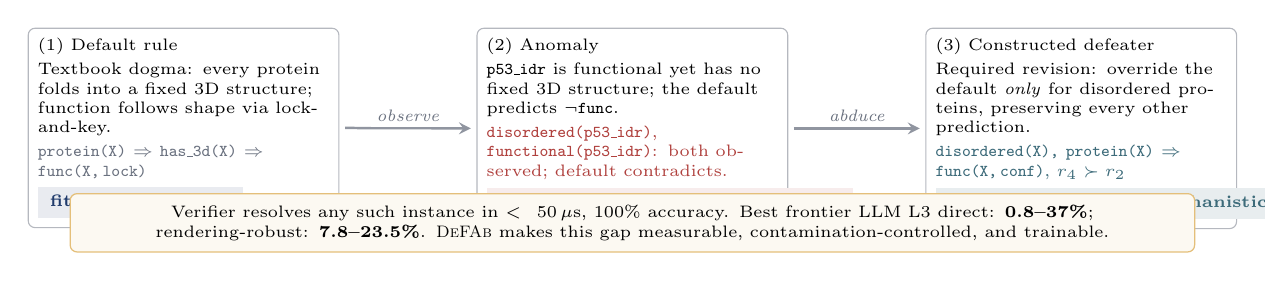
\begin{tikzpicture}[
    >=stealth,
    panel/.style={
        draw=defabGray!50, rounded corners=2.5pt,
        font=\fontsize{5.8}{6.9}\selectfont,
        inner sep=3.5pt, align=left, fill=white,
        line width=0.4pt,
        text width=3.7cm, minimum height=1.6cm, anchor=north
    },
    titlea/.style={
        font=\fontsize{7.5}{9}\selectfont\bfseries\color{defabBlue}
    },
    titleb/.style={
        font=\fontsize{7.5}{9}\selectfont\bfseries\color{defabRed}
    },
    titlec/.style={
        font=\fontsize{7.5}{9}\selectfont\bfseries\color{defabTeal}
    },
    badge/.style={
        font=\fontsize{5.6}{6.6}\selectfont\bfseries,
        inner sep=2pt, rounded corners=1.5pt
    },
    flow/.style={->, thick, color=defabGray!75, line width=0.9pt,
                 shorten >=2pt, shorten <=2pt},
    flowlbl/.style={
        font=\fontsize{6}{7}\selectfont\itshape,
        text=defabGray, fill=white, inner sep=2pt
    },
    verdict/.style={
        draw=defabGold!70, rounded corners=2.5pt,
        font=\fontsize{6.2}{7.4}\selectfont,
        inner sep=4pt, align=center, fill=defabGold!7,
        line width=0.45pt, text width=14.0cm,
        minimum height=0.7cm, anchor=north
    },
]

%% =================================================================
%% Panel A: The default (textbook biology)
%% =================================================================
\node[panel] at (-5.7, 0) (pa) {%
  {\titlea (1) Default rule}\\[2pt]
  Textbook dogma: every protein folds into a fixed 3D structure; function follows shape via lock-and-key.\\[2pt]
  {\fontsize{5.8}{6.8}\selectfont\color{defabGray}\texttt{protein(X)} $\Rightarrow$ \texttt{has\_3d(X)} $\Rightarrow$ \texttt{func(X,\,lock)}}\\[2pt]
  \colorbox{defabBlue!10}{\textcolor{defabBlue}{\bfseries\,fits PDB pre-1996\,}}%
};

%% =================================================================
%% Panel B: The anomaly (p53 IDR observation)
%% =================================================================
\node[panel] at (0.0, 0) (pb) {%
  {\titleb (2) Anomaly}\\[2pt]
  \texttt{p53\_idr} is functional yet has no fixed 3D structure; the default predicts $\lnot$\texttt{func}.\\[2pt]
  {\fontsize{5.8}{6.8}\selectfont\color{defabRed}\texttt{disordered(p53\_idr)}, \texttt{functional(p53\_idr)}: both observed; default contradicts.}\\[2pt]
  \colorbox{defabRed!10}{\textcolor{defabRed}{\bfseries\,prediction contradicts observation\,}}%
};

%% =================================================================
%% Panel C: The constructed defeater
%% =================================================================
\node[panel] at (5.7, 0) (pc) {%
  {\titlec (3) Constructed defeater}\\[2pt]
  Required revision: override the default \emph{only} for disordered proteins, preserving every other prediction.\\[2pt]
  {\fontsize{5.8}{6.8}\selectfont\color{defabTeal}\texttt{disordered(X), protein(X)} $\Rightarrow$ \texttt{func(X,\,conf)},\ $r_4 \succ r_2$}\\[2pt]
  \colorbox{defabTeal!12}{\textcolor{defabTeal}{\bfseries\,conservative, novel, mechanistic\,}}%
};

%% =================================================================
%% Inter-panel arrows
%% =================================================================
\draw[flow] (pa.east) -- node[flowlbl, above] {observe} (pb.west);
\draw[flow] (pb.east) -- node[flowlbl, above] {abduce} (pc.west);

%% =================================================================
%% Verdict strip (gap-of-capability summary)
%% =================================================================
\node[verdict] at (0, -2.10) (v) {%
  Verifier resolves any such instance in $<\!50\,\mu$s, 100\% accuracy. Best frontier LLM L3 direct: \textbf{0.8--37\%}; rendering-robust: \textbf{7.8--23.5\%}. \textsc{DeFAb} makes this gap measurable, contamination-controlled, and trainable.%
};

\end{tikzpicture}
}
\caption{The intrinsically disordered protein (IDP) discovery as a defeater abduction, illustrating the task DeFAb measures and trains for. (1)~textbook default: proteins fold into 3D structures that determine function. (2)~anomaly: \texttt{p53\_idr} is functional yet disordered, contradicting the default's prediction. (3)~required revision: a new rule that overrides the default \emph{only} for disordered proteins and posits a new mechanism (conformational ensembles). The polynomial-time verifier resolves any such instance in microseconds; frontier LLMs do not.}
\label{fig:intuition}
\end{figure}

This failure reflects three entangled deficits in current foundation models. The first is a \textit{grounding deficit}: models lack an explicit epistemic structure distinguishing strict knowledge from revisable defaults, and cannot trace predictions to their supporting evidence (the root cause of hallucination). The second is a \textit{novelty deficit}: without knowing which beliefs are revisable, models cannot identify where creative exceptions might apply. The IDP discovery is hard for an AI precisely because the default ``proteins have stable 3D structure'' is not flagged as revisable anywhere in the model's representations. The third, and least recognized, is a \textit{belief revision deficit}: even when models do update their knowledge (through in-context learning, fine-tuning, or explicit editing methods such as ROME \cite{meng2022locating} and MEMIT \cite{meng2023mass}), they lack the formal machinery to ensure that changes satisfy the principle of minimal change \cite{alchourron1985logic, dalal1988investigations}: accommodating new evidence while disturbing as few existing commitments as possible. Without this principle, updating one fact risks cascading incoherence, precisely the ``ripple effect'' problem documented in knowledge editing evaluations \cite{cohen2024evaluating}. The IDP discovery illustrates all three: the creative act requires not merely asserting that disordered proteins exist, but doing so via a targeted revision that overrides the structure--function default for a specific subclass while leaving predictions about conventionally structured proteins intact.

These deficits are mutually reinforcing. A model without grounding cannot perform targeted revision because it cannot identify what supports the conclusion to be revised. A model without rational revision machinery cannot be genuinely creative because proposed exceptions may resolve one anomaly while introducing others. And a model that cannot generate novel exceptions cannot revise its knowledge at all, only extend it monotonically. The common structural absence is an explicit \emph{defeasible knowledge structure}: one that marks which rules are strict versus revisable, traces every conclusion to its support set, and enables targeted revision with formal conservativity guarantees.

\textit{Defeasible reasoning} provides exactly this structure. In a defeasible theory, every conclusion is derived through a traceable chain of strict and defeasible rules, every default is explicitly revisable, and every piece of evidence participates in identifiable support sets. This provides grounding (one can determine \emph{why} the theory concludes what it does), the machinery for novelty (anomalous observations identify which defeasible rules to target), and a concrete operationalization of rational belief revision: our conservativity requirement (Definition~\ref{def:resstrength}) ensures that resolutions preserve all expectations except the targeted anomaly, directly implementing AGM's minimal change postulate \cite{gardenfors1988knowledge, katsuno1991propositional}; our revision distance metric (Definition~\ref{def:resstrength}) quantifies departure from this principle; and our graded scoring function (Section~\ref{subsec:partial_credit}) decomposes model failures along the stages of rational revision, from syntactic well-formedness through anomaly resolution to full conservativity.

This framework has deep roots in the philosophy of science. Popper~\cite{popper1959logic} argued that ``in so far as a scientific statement speaks about reality, it must be falsifiable: and in so far as it is not falsifiable, it does not speak about reality.'' A theory's empirical content is defined by its \emph{potential falsifiers}: ``the class of all those basic statements with which it is inconsistent (or which it rules out, or prohibits).'' In our formalization, defeasible rules are precisely Popperian conjectures---revisable claims whose content is defined by the defeaters that could override them. A defeasible rule with no possible defeater is unfalsifiable and contributes nothing to the theory's revisable knowledge; the richer the defeater set, the more the rule ``speaks about reality.''

Lakatos~\cite{lakatos1976proofs} refined this picture for mathematics in \emph{Proofs and Refutations}, identifying a four-stage cycle that maps directly onto our framework: ``1.~Primitive conjecture. 2.~Proof (a rough thought-experiment or argument, decomposing the primitive conjecture into subconjectures or lemmas). 3.~`Global' counterexamples emerge. 4.~Proof re-examined: the `guilty lemma' to which the global counterexample is a `local' counterexample is spotted. This guilty lemma may have previously remained `hidden' or may have been misidentified. Now it is made explicit, and built into the primitive conjecture as a condition. The theorem---the improved conjecture---supersedes the primitive conjecture with the new proof-generated concept as its paramount new feature.'' This is exactly the structure of our Level~3 task. The primitive conjecture is the defeasible rule. The counterexample is the anomaly $\alpha$. The guilty lemma is the missing condition that distinguishes the exception from the default case. The improved conjecture is the conservative defeater that supersedes the original rule for the exception class while preserving its validity elsewhere. Our conservativity requirement (Definition~\ref{def:resstrength}) formalizes Lakatos's demand that the improved theorem preserve the valid core of the original conjecture, and the graded scoring function decomposes model failures along the stages of this cycle.

A literary analogy clarifies this framework and will serve as a running example throughout the paper. Consider Agatha Christie constructing \emph{Murder on the Orient Express}~\cite{christie1934murder}. Christie possesses the complete theory $\Dfull$: she knows that twelve passengers, each secretly connected to the murdered Armstrong family, conspired to kill the disguised kidnapper Cassetti, each delivering one of twelve stab wounds in a locked compartment on a snowbound train. This complete knowledge (every motive, every alibi, every physical clue) constitutes a defeasible theory in which every conclusion has a traceable support set and every default is explicitly revisable.

To construct the mystery, Christie performs precisely the ablation operation of our benchmark: she withholds critical elements from $\Dfull$ to produce the challenge theory $\Dm$ that the detective Poirot receives. At Level~1, she hides individual facts: a burned letter revealing the victim's true identity, a conductor's button found in the compartment, a stopped watch establishing the time of death. These are ground facts whose absence renders specific conclusions underivable; the detective must abduce the missing observation. At Level~2, she conceals the rule connecting all twelve passengers to the Armstrong household: a missing generalization the detective must reconstruct from scattered evidence, just as a model must reconstruct a missing defeasible rule from the ablated theory.

Level~3 is where the analogy becomes most revealing. The default rule in any detective's reasoning is a deeply held generalization: ``murders are committed by a single perpetrator.'' This is a defeasible rule that the detective's entire training distribution reinforces. The anomaly $\alpha$ is the evidence contradicting every single-perpetrator hypothesis: twelve stab wounds of varying depth and angle, each passenger possessing both motive and partial alibi, a sealed train admitting no external intruder. Resolution requires constructing a \emph{defeater} (an exception rule asserting that all twelve passengers acted in concert) that overrides the single-perpetrator default. Crucially, this defeater must be \emph{conservative}: it must resolve the specific anomaly (the twelve wounds, the universal connection to Armstrong) without disrupting other established conclusions (the train's schedule, the snowdrift, the compartment layout). A non-conservative resolution, say, proposing that an outsider entered through a window, would contradict the established fact of the sealed, snowbound train and would score only $0.5$ in our graded evaluation: anomaly resolved, but minimal change violated.

In this analogy, legacy knowledge bases play Christie's role: the all-knowing author whose complete theory provides the ground truth from which we generate mysteries (ablated instances) and against which we verify solutions (the gold-standard computation of Section~\ref{subsec:abduction}). Foundation models play Poirot's role: they receive the incomplete theory and must abduce what is missing. The polynomial-time verifier of Section~\ref{subsec:abduction} is Christie's omniscience: the oracle that separates correct solutions from incorrect ones. Our benchmark measures whether models can progress from finding clues (Level~1) through discovering hidden rules (Level~2) to overriding deeply held defaults with conservative exceptions (Level~3): the progression from competent investigation to transformational, rationally creative insight.

Current benchmarks leave this space largely untested. Tasks like entailment verification \cite{tafjord2021proofwriter} and proof checking evaluate forward, monotonic reasoning. Knowledge editing benchmarks such as CounterFact \cite{meng2022locating} measure whether a target fact changed but rely on ad hoc heuristics for side-effect assessment rather than formally verifying conservativity. What is missing is a principled method for generating grounded abductive instances: one that combines the expressivity of defeasible logic with verifiable gold-standard answers and formal revision guarantees.

This creates what we term the \textit{tautological bottleneck}: the very hypotheses a model would need to generate are precisely those it has never seen, because the act of proposing them is what converts them from creative conjectures into textbook facts. But the bottleneck has a converse that is equally problematic: for the well-documented defaults and exceptions that \emph{do} appear in textbooks, we face a \textit{contamination confound}. When a model correctly identifies that penguins cannot fly or that metallic glasses are not brittle, we cannot distinguish genuine defeasible reasoning from retrieval of memorized training-corpus solutions. Recent work has quantified this risk: GSM1K \cite{zhang2024gsm1k} demonstrated accuracy drops of up to 8\% when grade-school math problems were regenerated to avoid training-set overlap, and LiveCodeBench \cite{jain2025livecodebench} showed that time-segmented evaluation reveals contamination even in frontier models. For defeasible reasoning benchmarks grounded in well-known knowledge bases (ConceptNet, Wikidata, YAGO), the risk is acute: many of the default--exception pairs (``birds fly'' / ``penguins do not fly'') are among the most commonly cited examples in AI textbooks and are almost certainly present verbatim in every frontier model's pretraining corpus.

To study both the tautological bottleneck and the contamination confound, we need a benchmark with five properties: (i)~formally verifiable gold-standard hypotheses, (ii)~controllable difficulty from gap-filling to creative exception-finding, (iii)~explicit grounding structure with traceable support sets and formal conservativity checks, (iv)~separation of logical reasoning from surface-form sensitivity, and (v)~\emph{contamination-resistant evaluation instances} whose solutions provably fall outside any pretraining corpus. Property~(v) is addressed by \emph{synthetic defeasible theories}: procedurally generated theories with invented predicate and entity names that preserve the formal structure of naturalistic theories (depth, branching, support set size, defeater complexity) while guaranteeing that no gold-standard hypothesis can be retrieved from memorized training data (Section~\ref{subsec:synthetic}).

Properties (i)--(iv) can be obtained by working backwards from existing structured knowledge bases; property~(v) is obtained by generating theories \emph{de novo} with the same pipeline (Section~\ref{subsec:synthetic}). The 1980s and 1990s produced large-scale, hand-engineered knowledge bases (Japan's Fifth Generation Computer Systems project, the UK's Alvey Programme, Cyc's million-axiom ontology \cite{lenat1990cyc}) that formalize domain expertise as logic programs. This tradition continued through subsequent government-funded programs: the NSF supported WordNet \cite{miller1995wordnet} and ConceptNet \cite{speer2017conceptnet}; the NIH assembled UMLS \cite{lindberg1993umls} and sponsored Gene Ontology \cite{ashburner2000go}; the EU funded LKIF Core for legal reasoning \cite{lkif2007} and BabelNet across 600 languages \cite{navigli2012babelnet}; and the US Materials Genome Initiative produced domain ontologies for materials science \cite{matonto2015}. In parallel, large-scale collaborative projects encoded encyclopedic knowledge with explicit exception structure: Wikidata's \texttt{exception-to-constraint} property (P2303) pairs community-curated rules with documented defeaters \cite{vrandecic2014wikidata}; DBpedia extracts typed relations monthly from Wikipedia across 140 languages \cite{lehmann2015dbpedia}; and YAGO integrates Wikidata with schema.org into a logically constrained taxonomy \cite{suchanek2024yago}. By converting this entire infrastructure into defeasible theories, we obtain structures in which every element's epistemic status, every conclusion's support set, and every default's vulnerability to exception are formally specified. From these structures we generate evaluation instances where the gold-standard answer is guaranteed by the complete theory but hidden from the model.

We introduce \textsc{DeFAb} (\textbf{De}feasible \textbf{A}bduction \textbf{B}enchmark), a dataset and generation pipeline grounded in this approach. Our contributions are:

\begin{enumerate}[label=(\arabic*),nosep]
    \item \textbf{A formal grounding framework} for converting definite logic programs into defeasible theories via a parameterized partition function $\kappa$ that controls which clauses are strict versus revisable. The resulting theories make epistemic commitments explicit: identifiable support sets, marked revisability, and polynomial-time criticality computation. The conversion is provably conservative when all clauses are strict (Proposition~\ref{prop:strict}).

    \item \textbf{A three-level evaluation hierarchy} testing grounding, novelty, and rational revision. Level~1 (fact completion) asks models to identify missing observations; Level~2 (rule abduction) asks models to reconstruct missing generalizations; Level~3 (defeater abduction) asks models to construct novel exception rules satisfying the conservativity constraint, performing rational belief revision in the defeasible setting. Gold-standard hypotheses are computed by a polynomial-time, verifier-backed pipeline (Corollary~\ref{cor:cubic}).

    \item \textbf{Controlled measures of novelty, revision, and difficulty.} Predicate novelty quantifies symbols introduced beyond the theory; revision distance (Definition~\ref{def:resstrength}) measures total cost in AGM-style minimal change; conservativity (Definition~\ref{def:resstrength}) verifies preservation of unrelated expectations. The graded scoring function (Section~\ref{subsec:partial_credit}) decomposes failures along the stages of rational belief revision.

    \item \textbf{A rendering-robust evaluation protocol.} Five modalities from narrative to raw syntax to visual grounding; the headline metric is worst-case accuracy across all text modalities, ensuring scores reflect epistemic reasoning rather than surface-form sensitivity.

    \item \textbf{A multimodal visual grounding modality (M5).} We extend the rendering protocol beyond text to visual entity grounding, replacing or supplementing textual entity identification with images harvested from linked knowledge bases (Wikidata P18, VisualSem, BabelNet). Two sub-variants---M5-replace, which hides entity names and requires visual perception, and M5-supplement, which pairs names with images---isolate perception from reasoning. This provides the first defeasible reasoning benchmark with formally verified gold standards for vision-language models, connecting to recent findings that VLMs systematically fail on atypical instances \cite{park2025visage}---precisely the defeasible case.

    \item \textbf{A cross-ontology KB extraction methodology} for generating defeasible rule bases at scale from heterogeneous publicly funded knowledge sources. The procedure pairs taxonomic hierarchies (OpenCyc, YAGO, Wikidata) with behavioral property graphs (ConceptNet, UMLS) to synthesize defeasible rules; exception relations (ConceptNet's \texttt{NotCapableOf}, Wikidata's P2303, Gene Ontology's \texttt{NOT}-qualified annotations) serve as structured defeater sources for Level~3, enabling automatic instance generation without manual authoring. A fifth structured partition family, the \emph{type-grounded} partition, maps relation type to epistemic status: taxonomic edges are strict, capability assertions are defeasible, and exception relations seed $\Rdf$ directly.

    \item \textbf{A synthetic contamination control.} We introduce procedurally generated \emph{synthetic defeasible theories} with invented predicate and entity names, preserving the structural parameters of naturalistic theories (depth, branching factor, support set size, defeater complexity) while guaranteeing that gold-standard hypotheses fall outside any pretraining corpus. The naturalistic--synthetic accuracy gap $\Delta_{\mathrm{synth}}$ provides a per-model, per-level upper bound on contamination-attributable performance inflation, and its absence constitutes positive evidence that measured accuracy reflects genuine defeasible reasoning capability rather than memorized solutions (Section~\ref{subsec:synthetic}).

    \item \textbf{A preference optimization pipeline for defeasible fine-tuning.} We present a method for converting DeFAb instances into verifier-grounded preference data for DPO~\cite{rafailov2023direct} and RLHF~\cite{ouyang2022training}, exploiting the benchmark's polynomial-time scoring function as an exact reward signal. The pipeline includes a margin-weighted DPO variant adapted to the ordinal structure of Level~3 graded scoring, a verifier-in-the-loop (VITL) RLHF variant that eliminates reward model approximation, and curriculum schedules informed by the level hierarchy (Section~\ref{sec:finetuning}).

    \item \textbf{A game-theoretic framework for defeasible conflict resolution.} We formalize defeasible conflicts as two-player zero-sum games whose outcomes produce structurally grounded preference pairs for DPO and self-play training signal for GRPO. The framework extends to a theory construction MDP in which the agent builds coherent theories through sequential actions, each verified in polynomial time, and an Active Inference formulation~\cite{parr2022active} that separates epistemic exploration (probing theory structure) from pragmatic revision (constructing defeaters). The formal properties of these games---binarity, zero-sumness, finiteness, and determinacy---are established in Appendix~\ref{app:game_theory} (Section~\ref{subsec:conflict_games}).

    \item \textbf{An adversarial defeasible debate protocol.} We formalize a competitive multi-agent evaluation framework in which two agents use Monte Carlo Tree Search over the derivation space to propose and defend competing conclusions. The Author Algorithm's criticality computation generates mutual challenges by permuting proof trees, and agents must defend under these adversarial perturbations. Resolution metrics for robustness, grounding, and creativity provide a richer diagnostic signal than single-pass evaluation (Section~\ref{sec:debate}).
\end{enumerate}

Returning to the IDP example: the default ``proteins have stable 3D structure'' is a defeasible rule $r_1$ with identifiable support and computable criticality. The discovery corresponds to constructing an exception rule $r_4$ (``disordered proteins function via conformational ensembles'') that overrides the default mechanism. Crucially, $r_4$ must be \emph{conservative}: resolving the anomaly for p53\_idr without disrupting predictions about conventionally structured proteins (the defeasible analogue of AGM's minimal change). A model that proposes $r_4$ but destabilizes unrelated predictions scores $0.5$; one that preserves all side-effects scores $1.0$. The benchmark thus measures not just whether a model can be creative, but whether it can be \emph{rationally} creative.

Section~\ref{sec:method} formalizes the pipeline, including the synthetic theory generation procedure for contamination control (Section~\ref{subsec:synthetic}); Section~\ref{sec:experiments} presents the experimental design with both naturalistic and synthetic evaluation conditions; Section~\ref{sec:finetuning} develops the preference optimization methodology for defeasible fine-tuning; Section~\ref{sec:debate} introduces the adversarial debate protocol; full definitions and proofs appear in the appendices.


\section{Related Work}\label{sec:related}
Non-monotonic reasoning has a rich formal history. Reiter's default logic \cite{reiter1980logic} and McCarthy's circumscription \cite{mccarthy1980circumscription} addressed the inadequacy of classical logic for commonsense reasoning, where new information routinely overrides prior conclusions. Nute's defeasible logic \cite{nute1987defeasible, nute1994defeasible} offered a computationally tractable alternative by distinguishing strict rules, defeasible rules, and defeaters, with subsequent applications to legal reasoning \cite{nute1997logic}. The KLM framework \cite{kraus1990nonmonotonic} provided axiomatic foundations for rational non-monotonic inference, and recent work by Dennison, Heyninck, and Meyer \cite{dennison2026rational} has enabled algorithmic computation of Rational Closure via Answer Set Programming. These formalisms provide the machinery for reasoning about defaults and exceptions, yet their integration with modern language models remains limited.

The formal semantics underlying our source theories rests on the model-theoretic foundations of logic programming established by van Emden and Kowalski \cite{vanemden1976semantics}, who showed that the semantics of definite logic programs can be characterized via a least fixed point of an immediate consequence operator. Lloyd \cite{lloyd1987foundations} provided the standard treatment of Herbrand models, SLD-resolution, and the monotonicity properties of definite programs that our conversion exploits. Kakas, Kowalski, and Toni \cite{kakas1992abductive} extended logic programming to abductive reasoning, introducing the framework of abductive logic programming in which hypotheses are generated to explain observations relative to an incomplete theory. Our instance generation procedure (Section~\ref{subsec:abduction}) adapts this paradigm: given an ablated theory $\Dm$ and an unexplained target $q$, the task is to abduce a minimal hypothesis $h$ restoring the derivation.

The proof theory we adopt for defeasible reasoning follows the formalization of Antoniou, Billington, Governatori, and Maher \cite{antoniou2001defeasible}, who established representation results, normal forms, and transformations for defeasible logic. Maher \cite{maher2001propositional} proved that propositional defeasible derivation has linear time complexity, a result that underlies the tractability of our generation pipeline. The ``team defeat'' mechanism in this proof theory, where every attacking rule must be individually neutralized, connects to Dung's \cite{dung1995acceptability} abstract argumentation frameworks, in which acceptability of arguments depends on defeating all attackers. Governatori, Maher, Antoniou, and Billington \cite{governatori2004argumentation} made this connection explicit by providing argumentation semantics for defeasible logic, showing that defeasible proof tags correspond to argument labellings. Our defeater abduction task (Section~\ref{subsec:level3}) requires models to construct arguments that defeat existing default inferences, operating within this argumentation-theoretic structure. The complexity results for our Defeater Abduction Problem draw on Eiter and Gottlob's \cite{eiter1995complexity} foundational analysis of abduction complexity, which established NP-completeness for propositional abduction and $\Sigma_2^P$-completeness for problems requiring universal quantification over counterexamples.

Our framework connects to the theory of belief revision initiated by Alchourr\'{o}n, G\"{a}rdenfors, and Makinson \cite{alchourron1985logic}, who established rationality postulates for how an ideal agent should update beliefs in response to new evidence. G\"{a}rdenfors \cite{gardenfors1988knowledge} developed the principle of minimal change, and Katsuno and Mendelzon \cite{katsuno1991propositional} provided model-theoretic characterizations. Dalal \cite{dalal1988investigations} introduced distance-based revision using Hamming distance between models. Our conservativity requirement (Definition~\ref{def:resstrength}) operationalizes minimal change in the defeasible setting, and our revision distance (Definition~\ref{def:resstrength}) provides a tractable analogue of Dalal's distance. This connection is practically significant: the knowledge editing literature (including ROME \cite{meng2022locating}, MEMIT \cite{meng2023mass}, and evaluations of their side effects \cite{cohen2024evaluating}) addresses belief revision in neural models but lacks formally grounded measures of conservativity. Our benchmark provides exactly such measures, bridging the gap between the formal revision theory and empirical evaluation of neural knowledge updates.

\paragraph{Philosophy of science.} The structure of defeasible reasoning reflects longstanding accounts of how scientific knowledge develops. Popper~\cite{popper1959logic} argued that ``bold ideas, unjustified anticipations, and speculative thought, are our only means for interpreting nature,'' and that ``whenever we propose a solution to a problem, we ought to try as hard as we can to overthrow our solution, rather than defend it.'' This characterizes both our Level~3 task (the model must propose a bold exception to an established default) and our adversarial debate protocol (Section~\ref{sec:debate}), where agents actively attempt to overthrow each other's derivations. Lakatos~\cite{lakatos1976proofs} extended Popperian falsificationism to mathematics, demonstrating through the history of Euler's polyhedron formula ($V - E + F = 2$) that mathematical concepts themselves evolve through counterexample-driven refinement. He identified three strategies for handling counterexamples: \emph{monster-barring} (excluding the counterexample from the definition), \emph{exception-barring} (acknowledging exceptions but carving them out), and \emph{lemma-incorporation} (identifying the specific hidden assumption the counterexample violates and making it explicit). These correspond to distinct defeater construction strategies in our framework: monster-barring produces defeaters that restrict the domain of the original rule; exception-barring produces defeaters that enumerate specific exception cases; lemma-incorporation produces defeaters that introduce a new condition distinguishing the exception from the default. Lakatos favored lemma-incorporation as the strategy that ``yields more information'' because it requires understanding \emph{why} the counterexample arises, not merely \emph{that} it exists. Our conservativity requirement operationalizes this preference: a lemma-incorporating defeater preserves more of the theory's expectations than a monster-barring defeater, and therefore achieves a higher conservativity score. Kuhn's paradigm shifts~\cite{kuhn1962structure}, in which anomalies accumulate until a scientific framework is replaced, correspond to cases where the defeater set grows large enough to warrant restructuring the theory rather than adding individual exceptions. These connections are not merely analogical; they suggest that the DeFAb pipeline extends naturally to formalized mathematics, where Lean~4 or Isabelle could replace the defeasible derivation checker and Mathlib formalizations could serve as the source theory (Section~\ref{sec:discussion}).

\paragraph{Neurosymbolic integration.} Recent neurosymbolic systems have begun to bridge the gap between formal reasoning and neural language models. LOGicalThought \cite{nananukul2025logicalt} translates natural language into RuleLog programs and feeds symbolic structure back into language models, achieving modest improvements on defeasible reasoning tasks. DARK \cite{gao2025dark} unifies deduction and abduction via masked diffusion over knowledge graphs, using a self-reflective cycle to generate and verify hypotheses. LLM-ASPIC+ \cite{fang2025llmaspic} combines language model grounding with formal ASPIC+ argumentation, achieving state-of-the-art accuracy on multi-step defeasible reasoning benchmarks by delegating conflict resolution to the symbolic layer. These systems share the goal of injecting formal structure into LLM reasoning pipelines, yet all remain evaluation-free in the benchmark sense: they develop new \emph{solvers} without providing the formally grounded \emph{instances} needed to evaluate whether models can construct defeaters or perform conservative belief revision. LogT focuses on forward reasoning (verifying conclusions) rather than abductive hypothesis generation; DARK's reliance on knowledge graph triples sacrifices the expressivity needed for complex exception handling; and LLM-ASPIC+ assumes the argumentation structure is given rather than abduced.

Concurrently, multi-agent debate has emerged as a promising paradigm for improving LLM reasoning. Irving, Christiano, and Amodei \cite{irving2018ai_safety_debate} proposed AI safety via debate, where two agents compete to convince a judge, providing a scalable oversight mechanism. Du et al.\ \cite{du2023debate} demonstrated that multi-agent debate improves factuality and reasoning by forcing models to confront conflicting perspectives. Tree of Thoughts \cite{yao2024tree_of_thoughts} applies tree search to LLM reasoning, achieving significant improvements on tasks requiring deliberate exploration. Monte Carlo Tree Search has been applied to LLM reasoning through ReST-MCTS* and related work, using process reward models for step-level verification. However, none of these approaches combine MCTS with formal defeasible reasoning or use argumentation-theoretic proof structures as the substrate for competitive exploration. Our debate protocol (Section~\ref{sec:debate}) bridges this gap: agents explore the derivation space of a defeasible theory via MCTS, and the Author Algorithm's criticality computation generates adversarial challenges grounded in the formal framework.

Orthogonal to the question of what benchmarks evaluate is the question of whether benchmark performance reflects genuine capability or memorized solutions. Zhang et al.\ \cite{zhang2024gsm1k} introduced GSM1K, a set of grade-school math problems regenerated to avoid overlap with the widely-used GSM8K training set, and demonstrated accuracy drops of up to 8\% attributable to contamination, with a positive correlation between a model's probability of generating GSM8K examples and its performance gap between the two benchmarks. LiveCodeBench \cite{jain2025livecodebench} addresses contamination in code evaluation through continuously collected problems with time-stamped release dates, enabling time-segmented evaluation that revealed contamination in both open and closed models. These results establish that pretraining data contamination is a systemic concern for any benchmark whose content overlaps with web-scale training corpora. For defeasible reasoning benchmarks grounded in well-known knowledge bases (ConceptNet, Wikidata, YAGO), the concern is especially acute: the canonical default--exception pairs that constitute gold-standard hypotheses are among the most frequently discussed examples in AI education and are almost certainly present verbatim in frontier models' pretraining data. Our synthetic contamination control (Section~\ref{subsec:synthetic}) addresses this by generating structurally isomorphic theories with invented predicate names verified for zero web-corpus overlap, providing the first contamination-resistant evaluation methodology for defeasible reasoning.

An emerging body of work extends abductive and defeasible reasoning evaluation to the multimodal setting. VISaGE \cite{park2025visage} evaluates how vision-language models handle visual generics and exceptions, revealing a systematic failure on atypical instances: when an image depicts an entity that violates the typical properties of its category (e.g., a flightless bird), VLMs degrade significantly relative to typical instances. This is precisely the defeasible case---atypical instances are those governed by defeater rules---yet VISaGE evaluates via crowdsourced annotations rather than formally specified defeasible theories. The Black Swan benchmark \cite{chinchure2025blackswan} tests abductive and defeasible reasoning in video, comprising over 15,400 questions across 1,655 videos of unexpected events, with state-of-the-art VLMs trailing human performance by up to 32 percentage points. AbductiveMLLM \cite{chang2026abductivemllm} addresses visual abductive reasoning via a Reasoner--Imaginer architecture that generates and prunes visual hypotheses through cross-modal causal alignment. In the biomedical domain, PhenoLIP \cite{liu2026phenolip} grounds medical VLMs in phenotype ontology structure, demonstrating that structured knowledge integration improves cross-modal retrieval; CardioKG \cite{rjoob2026cardiokg} integrates vision-derived cardiovascular phenotypes with biological knowledge graphs. Babel-ImageNet \cite{geigle2024babelimagenet} provides the infrastructure for linking BabelNet synsets to ImageNet images via shared WordNet mappings, enabling multilingual and multimodal concept grounding. These systems share a limitation that our M5 modality (Section~\ref{subsec:rendering}) addresses: none provides formally verified gold standards for multimodal defeasible reasoning. DeFAb-M5 pairs the visual grounding challenge with the benchmark's polynomial-time verifier, producing the first multimodal defeasible reasoning evaluation with verifier-backed correctness guarantees.

Existing benchmarks reinforce this asymmetry. ProofWriter \cite{tafjord2021proofwriter} and LogicNLI \cite{tian2021diagnosing} evaluate deductive verification: given premises, determine truth values. The inverse problem, generating the missing premise that would license a given conclusion, remains underexplored. The INABHYD benchmark \cite{inabhyd2025} demonstrates that language models fail to follow Occam's Razor in abductive contexts, systematically hallucinating unnecessary entities when simpler explanations suffice. LogiDynamics \cite{zheng2025logidynamics} studies the interplay of inductive, abductive, and deductive inference in LLMs, finding that System~2 strategies (hypothesis selection and iterative refinement) substantially improve performance on complex multi-step problems, but evaluates over generic analogical tasks rather than formally specified defeasible theories. LLM-ORBench \cite{llmorbench2026} evaluates ontology-based deductive inference via SPARQL, but similarly does not address hypothesis construction or defeasibility.

The closest related work on defeasible reasoning evaluation is \textsc{DeFReasing} \cite{allaway2025defreasing}, which probes whether language models correctly handle property inheritance in the presence of exceptions, using generics (quantifier-free generalizations such as ``birds fly'') as its rule representation. The dataset contains approximately 95,000 questions over around 8,000 inheritance rules, with the best models achieving only 0.64 F1 overall. Our benchmark differs from \textsc{DeFReasing} in three fundamental ways. First, \textsc{DeFReasing} is a \emph{classification} task (given additional information, does the property still hold?) while \textsc{DeFAb} is a \emph{construction} task: the model must generate the exception rule, receiving no candidate at Level~3. Second, \textsc{DeFReasing} uses natural language generics with human-annotated semantics; \textsc{DeFAb} uses formally specified defeasible theories with verifier-backed gold standards computable from complete theories, making correctness decidable in polynomial time. Third, and most critically, \textsc{DeFReasing} contains no formal analog of conservativity: it does not test whether a model's proposed revision preserves unrelated expectations. Our graded scoring function and revision distance directly measure this, operationalizing the AGM minimal-change postulate in a way that \textsc{DeFReasing} does not attempt. What is missing from the benchmark landscape is a principled method for generating grounded abductive evaluation instances with formally verifiable gold-standard answers and conservativity guarantees, which \textsc{DeFAb} provides.

The 1980s witnessed an unprecedented international investment in knowledge-based systems, producing large-scale knowledge bases that remain underutilized for modern foundation model research. Japan's Fifth Generation Computer Systems project, launched in 1982 by MITI, aimed to develop computers capable of knowledge information processing through logic programming and parallel inference \cite{fuchi1984aiming, feigenbaum1993fgcs}. This initiative catalyzed competitive responses worldwide: the UK's Alvey Programme (1983--1990) focused on Intelligent Knowledge-Based Systems \cite{alvey1985ikbs}, and DARPA's Strategic Computing Initiative tripled US investment in AI between 1984 and 1988. Concurrently, the Cyc project began at MCC in 1984, eventually assembling over $10^6$ handcrafted axioms and developing CycL, a representation language with explicit support for default reasoning and non-monotonic inference \cite{lenat1990cyc, lenat1995cyc}. While these initiatives are often characterized as commercial failures, they produced substantial artefacts: formal ontologies, rule bases distinguishing strict from defeasible knowledge, and inference engines designed for reasoning under incomplete information. This tradition of publicly funded knowledge engineering continued into subsequent decades through domain-specific programs: the NIH's Unified Medical Language System \cite{lindberg1993umls} now integrates 3.4 million medical concepts from 189 source vocabularies; the NSF-funded WordNet \cite{miller1995wordnet} and ConceptNet \cite{speer2017conceptnet} encoded lexical and commonsense knowledge at scale; the US Materials Genome Initiative produced structured materials ontologies \cite{matonto2015}; and the EU's ESTRELLA project delivered LKIF Core for legal knowledge interchange \cite{lkif2007}. Simultaneously, collaborative encyclopedic projects assembled billions of typed structured assertions: Wikidata \cite{vrandecic2014wikidata} with 16.6 billion RDF statements and an explicit constraint--exception mechanism (P2302/P2303); DBpedia \cite{lehmann2015dbpedia} with monthly extractions from 140 Wikipedias; YAGO \cite{suchanek2024yago} combining Wikidata with schema.org under enforced logical constraints; and BabelNet \cite{navigli2012babelnet} integrating 53 knowledge sources across 600 languages. These systems collectively encode not only default generalizations but also documented exceptions, making them natural sources for both defeasible rules and structured defeaters. Our work provides the first systematic pipeline for converting this entire infrastructure into formally grounded defeasible abduction benchmarks, with a staged extraction methodology (Section~\ref{subsec:sources}) that scales from thousands of expert-curated instances to millions as additional sources are incorporated.


\section{Our Method}\label{sec:method}

Our approach addresses the three deficits identified in Section~1 (grounding, novelty, and belief revision) by constructing evaluation instances from knowledge bases whose epistemic structure is fully explicit. The pipeline has four stages: (1)~formalizing legacy knowledge bases as definite logic programs, whose monotonic semantics provides a complete ground truth; (2)~converting them into defeasible theories via a parameterized transformation that makes the strict/default distinction explicit, giving every conclusion a traceable support set; (3)~generating abductive evaluation instances by systematically ablating elements of these theories, producing tasks that require grounded reasoning (Levels~1--2) or rational belief revision (Level~3); and (4)~rendering the resulting tasks into natural language for evaluation of foundation models. We present the essential definitions and constructions here; full proofs and extended formalisms appear in Appendices~\ref{app:definitions}--\ref{app:rendering}. In terms of the Orient Express analogy introduced in Section~1: Stage~(1) formalizes Christie's complete knowledge as a logic program; Stage~(2) marks which of her knowledge is strict fact versus revisable default; Stage~(3) constructs the mystery by ablating critical elements; and Stage~(4) presents the puzzle to the detective in readable form.


Figure~\ref{fig:pipeline} illustrates the end-to-end pipeline on the running bear-hibernation theory across all three task levels.

\begin{figure}[t]
\centering
\resizebox{\textwidth}{!}{% DeFAb combined pipeline + L1/L2/L3 generation figure
%
% Fixed-grid layout with conservative row heights:
%   Every row uses anchor=north with an ABSOLUTE y coordinate.
%   minimum height is set ≥ actual content height so boxes never overflow.
%
%   Row y-coordinates (top of box):
%     Pipeline arc :  y = 0.00
%     Level headers :  y = −1.05   (height 0.40cm → bottom −1.45)
%     Theory boxes  :  y = −1.60   (height 0.90cm → bottom −2.50)  3 lines max
%     Ablated boxes :  y = −2.65   (height 0.70cm → bottom −3.35)  2 lines max
%     Gold boxes    :  y = −3.50   (height 0.45cm → bottom −3.95)  1 line
%     Distractor    :  y = −4.10   (height 0.40cm → bottom −4.50)  1 line
%     Modality      :  y = −4.65   (height 0.60cm → bottom −5.25)  M5 taller
%     Caption label :  y = −5.40
%
%   Column x-centres: L1=−3.50, L2=0, L3=+3.50
%
\begin{tikzpicture}[
    >=stealth,
    %--- pipeline top row ---
    pipebox/.style={
        draw=defabBlue!70, rounded corners=2pt,
        font=\fontsize{6.2}{7.2}\selectfont,
        inner sep=3pt, text centered, align=center,
        fill=defabBlue!6, line width=0.4pt,
        minimum height=0.54cm, text width=1.30cm
    },
    %--- column headers ---
    levhdr/.style={
        draw=defabTeal!70, rounded corners=2pt,
        font=\fontsize{6.5}{7.5}\selectfont\bfseries,
        inner sep=2.5pt, text centered, align=center,
        fill=defabTeal!12, line width=0.4pt,
        text width=3.2cm, minimum height=0.40cm,
        anchor=north, text=defabTeal
    },
    %--- theory box (3 lines strict) ---
    tbox/.style={
        draw=defabGray!45, rounded corners=1.5pt,
        font=\fontsize{5.6}{6.6}\selectfont,
        inner sep=2.5pt, align=left,
        fill=white, line width=0.35pt,
        text width=3.2cm, minimum height=0.90cm, anchor=north
    },
    %--- ablated element box (2 lines, red) ---
    abox/.style={
        draw=defabRed!65, rounded corners=1.5pt,
        font=\fontsize{5.6}{6.6}\selectfont\bfseries,
        inner sep=2.5pt, align=left,
        fill=defabRed!7, line width=0.45pt,
        text width=3.2cm, minimum height=0.70cm,
        anchor=north, text=defabRed
    },
    %--- gold answer box (1 line, teal) ---
    gbox/.style={
        draw=defabTeal!70, rounded corners=1.5pt,
        font=\fontsize{5.6}{6.6}\selectfont\bfseries,
        inner sep=2.5pt, align=left,
        fill=defabTeal!9, line width=0.40pt,
        text width=3.2cm, minimum height=0.45cm,
        anchor=north, text=defabTeal!85
    },
    %--- distractor box (1 line, gray italic) ---
    dbox/.style={
        draw=defabGray!35, rounded corners=1.5pt,
        font=\fontsize{5.4}{6.2}\selectfont\itshape,
        inner sep=2.5pt, align=left,
        fill=defabGray!4, line width=0.30pt,
        text width=3.2cm, minimum height=0.40cm,
        anchor=north, text=defabGray
    },
    %--- modality boxes (gold border) ---
    mbox/.style={
        draw=defabGold!70, rounded corners=2pt,
        font=\fontsize{6.0}{7.0}\selectfont,
        inner sep=2.5pt, text centered, align=center,
        fill=defabGold!8, line width=0.4pt,
        text width=3.0cm, anchor=north
    },
    %--- image placeholder (for M5 example) ---
    imgbox/.style={
        draw=defabGold!60, rounded corners=1pt,
        font=\fontsize{5.0}{5.8}\selectfont\bfseries,
        inner sep=1.5pt, text centered, align=center,
        fill=defabGold!12, line width=0.5pt,
        minimum width=0.7cm, minimum height=0.42cm,
        text=defabGold!80
    },
    %--- arrows ---
    parr/.style={->, thick, color=defabBlue!55, line width=0.6pt},
    sarr/.style={->, thin, color=defabGray!60, line width=0.40pt},
]

%% ============================================================
%% PIPELINE ARC  (top row, centred)
%% ============================================================
\node[pipebox] (kb) at (-5.10, 0)
    {KBs\\{\fontsize{5}{6}\selectfont\color{defabGray}15+ srcs}};
\node[pipebox, right=0.45cm of kb] (lp) {Logic\\Program $\Pi$};
\node[pipebox, right=0.45cm of lp] (dt) {Defeasible\\Theory $\D$};
\node[pipebox, right=0.45cm of dt] (ab) {Ablate\\$e$};
\node[pipebox, right=0.45cm of ab] (vr) {\textbf{Verifier}\\$O(|\D|^3)$};

\draw[parr] (kb) -- node[above,font=\fontsize{4.8}{5.8}\selectfont\itshape,
    text=defabGray,inner sep=1pt]{form.} (lp);
\draw[parr] (lp) -- node[above,font=\fontsize{4.8}{5.8}\selectfont\itshape,
    text=defabGray,inner sep=1pt]{$\kappa$} (dt);
\draw[parr] (dt) -- node[above,font=\fontsize{4.8}{5.8}\selectfont\itshape,
    text=defabGray,inner sep=1pt]{ablate} (ab);
\draw[parr] (ab) -- node[above,font=\fontsize{4.8}{5.8}\selectfont\itshape,
    text=defabGray,inner sep=1pt]{verify} (vr);

%% ============================================================
%% LEVEL HEADERS  (top at y = −1.05)
%% ============================================================
\node[levhdr] at (-3.50,-1.05) (h1) {L1: Fact Completion};
\node[levhdr] at (  0.00,-1.05) (h2) {L2: Rule Abduction};
\node[levhdr] at (  3.50,-1.05) (h3) {L3: Defeater Abduction};

%% ============================================================
%% ROW 1 — Theory boxes  (top at y = −1.60, min-height 0.90cm)
%% All columns have exactly 3 content lines
%% ============================================================
\node[tbox] at (-3.50,-1.60) {
  \textbf{Theory:} \texttt{bear(G)\ bear(P)\ arc(P)}\\
  $r_d$: \texttt{bear(X)$\Rightarrow$hib(X)}\\
  $r^*$: \texttt{bear(X),arc(X)$\leadsto\neg$hib}
};
\node[tbox] at ( 0.00,-1.60) {
  \textbf{Theory:} \texttt{bear(G)\ bear(P)\ arc(P)}\\
  $r_s$: \texttt{bear(X)$\to$mammal(X)}\\
  $r^*$: \texttt{bear(X),arc(X)$\leadsto\neg$hib}
};
\node[tbox] at ( 3.50,-1.60) {
  \textbf{Theory:} \texttt{bear(P)\ arc(P)\ seal(P)}\\
  \texttt{winter\_active(P)}\\
  $r_d$: \texttt{bear(X)$\Rightarrow$hib(X)}
};

%% ============================================================
%% ROW 2 — Ablated boxes  (top at y = −2.65, min-height 0.70cm)
%% 2 content lines per box
%% ============================================================
\node[abox] at (-3.50,-2.65) {
  \textbf{Remove:} \texttt{bear(grizzly)}\\
  Target \texttt{hib(G)}: chain broken!
};
\node[abox] at ( 0.00,-2.65) {
  \textbf{Remove:} $r_d$: \texttt{bear(X)$\Rightarrow$hib}\\
  Target \texttt{hib(G)}: no rule!
};
\node[abox] at ( 3.50,-2.65) {
  \textbf{Remove:} $r^*$ — now $r_d$ fires\\
  $\Rightarrow$\texttt{hib(polar)}: \textbf{anomaly!}
};

%% ============================================================
%% ROW 3 — Gold answer boxes  (top at y = −3.50, min-height 0.45cm)
%% ============================================================
\node[gbox] at (-3.50,-3.50) {
  \textbf{Gold:} \texttt{bear(grizzly)} (restores)
};
\node[gbox] at ( 0.00,-3.50) {
  \textbf{Gold:} \texttt{bear(X)$\Rightarrow$hib(X)}
};
\node[gbox] at ( 3.50,-3.50) {
  \textbf{Score 1.0:} $r^*$ restored; $r^*\!\succ\!r_d$
};

%% ============================================================
%% ROW 4 — Distractor boxes  (top at y = −4.10, min-height 0.40cm)
%% ============================================================
\node[dbox] at (-3.50,-4.10) (d1) {
  Distractor: \texttt{mammal(G)} [wrong pred.]
};
\node[dbox] at ( 0.00,-4.10) (d2) {
  Distractor: \texttt{mammal(X)$\Rightarrow$hib} [too broad]
};
\node[dbox] at ( 3.50,-4.10) (d3) {
  Score 0.5: \texttt{$\neg$hib(X):- bear(X)} [not conserv.]
};

%% ============================================================
%% ROW 5 — Modality boxes  (top at y = −4.65, height varies)
%% M5 box is taller to show visual-grounding schematic
%% ============================================================
\node[mbox, minimum height=0.42cm] at (-3.50,-4.65) (m1) {M1 Narrative};
\node[mbox, minimum height=0.42cm] at ( 0.00,-4.65) (m2) {M2--M4 Formal};

%% M5 box with embedded image-placeholder schematic
\node[mbox, minimum height=0.72cm, text width=3.0cm] at (3.50,-4.65) (m3) {
  M5: Visual Grounding\\[-1pt]
  \texttt{bear(P).}\ $\to$\
  \begin{tikzpicture}[baseline=-1pt]
    \draw[defabGold!60, rounded corners=0.8pt, line width=0.45pt,
          fill=defabGold!12]
        (0,0) rectangle (0.72cm,0.36cm);
    \node[font=\fontsize{4.6}{5}\selectfont\bfseries,
          text=defabGold!80] at (0.36cm,0.18cm) {IMG};
    % small camera corner marks
    \draw[defabGold!50, line width=0.3pt] (0.05cm,0.30cm)
        -- (0.05cm,0.31cm) -- (0.12cm,0.31cm);
    \draw[defabGold!50, line width=0.3pt] (0.67cm,0.31cm)
        -- (0.67cm,0.30cm);
  \end{tikzpicture}
};

\draw[sarr] (d1.south) -- (m1.north);
\draw[sarr] (d2.south) -- (m2.north);
\draw[sarr] (d3.south) -- (m3.north);

%% horizontal sibling arrows between modality boxes
\draw[{<[scale=0.55]}-{>[scale=0.55]}, color=defabGold!65, line width=0.4pt]
    (m1.east) -- (m2.west);
\draw[{<[scale=0.55]}-{>[scale=0.55]}, color=defabGold!65, line width=0.4pt]
    (m2.east) -- (m3.west);

\node[font=\fontsize{5.0}{6}\selectfont\itshape, text=defabGold!80,
      anchor=north] at (0,-5.42)
    {Any instance rendered in five modalities (M5 replaces entity names with images)};

%% ============================================================
%% Arrows: pipeline ablation box → column headers
%% ============================================================
\draw[sarr] (ab.south) ..controls +(-0.30,-0.28) and +(0.12,0.30).. (h1.north);
\draw[sarr] (ab.south) -- (h2.north);
\draw[sarr] (ab.south) ..controls +(0.30,-0.28) and +(-0.12,0.30).. (h3.north);

\end{tikzpicture}
}
\caption{The DeFAb generation pipeline and per-level instance structure. \textbf{Top:} Legacy knowledge bases are converted to defeasible theories via partition function $\kappa$; a critical element is ablated and the polynomial-time verifier ($O(|\D|^3)$) certifies the gold hypothesis. \textbf{Bottom:} The same bear-hibernation theory, ablated three ways. \emph{Level~1} removes the fact \texttt{bear(grizzly)}: the model must identify the missing observation. \emph{Level~2} removes the defeasible rule $r_d$: the model reconstructs the missing generalization; the distractor \texttt{mammal(X)$\Rightarrow$hib(X)} is tempting but too broad. \emph{Level~3} removes the defeater $r^*$: the theory now incorrectly predicts \texttt{hib(polar\_bear)} despite \texttt{winter\_active(polar\_bear)}; the model must \emph{construct} a conservative exception rule (Score~1.0), not a broad one that destroys other predictions (Score~0.5). Any generated instance can be rendered in five modalities (M1--M5).}
\label{fig:pipeline}
\end{figure}


\subsection{Source Theories}\label{subsec:source}

We formalize legacy knowledge bases (Cyc, FGCS-era Prolog programs, Alvey artefacts) as definite logic programs over a first-order signature $\Sigma = (\mathcal{C}, \mathcal{F}, \mathcal{P})$ of constants, function symbols, and predicate symbols. A definite logic program $\Pi$ is a finite set of clauses $h \leftarrow b_1, \ldots, b_n$ ($n \geq 0$), where facts have $n = 0$. Its semantics is given by the least Herbrand model $\mathcal{M}_\Pi = \mathrm{lfp}(T_\Pi)$, the least fixed point of the immediate consequence operator (Definitions~\ref{def:signature}--\ref{def:lhm}). The property we exploit is monotonicity: $\Pi \subseteq \Pi'$ implies $\mathcal{M}_\Pi \subseteq \mathcal{M}_{\Pi'}$. Adding clauses can only increase the set of derivable conclusions. This is precisely the limitation our framework addresses: monotonic theories cannot retract defaults in light of new evidence, and thus cannot model the belief revision that transformational scientific discovery requires.


\subsection{Defeasible Conversion}\label{subsec:conversion}

A defeasible theory $\D = (F, \Rs, \Rd, \Rdf, {\succ})$ consists of facts $F$, strict rules $\Rs$ (invariable), defeasible rules $\Rd$ (revisable defaults), defeaters $\Rdf$ (rules that block but cannot support conclusions), and an acyclic superiority relation $\succ$ resolving conflicts (Definition~\ref{def:deftheory}). A literal $q$ is defeasibly provable, written $\D \pPartial q$, when there exists an applicable defeasible rule for $q$ and every attacking rule for $\comp{q}$ is either inapplicable or overridden by a superior rule (Definition~\ref{def:defderiv}).

We convert a definite logic program $\Pi$ into a defeasible theory via a partition function $\partfunc: \Pi \to \{s, d\}$ that classifies each clause as strict or defeasible:
\begin{equation}\label{eq:conversion}
    \phi_\partfunc(\Pi) = (F_\partfunc,\; \Rs^{\partfunc},\; \Rd^{\partfunc},\; \emptyset,\; \emptyset).
\end{equation}
Clauses assigned $s$ become facts or strict rules; clauses assigned $d$ become defeasible rules. The conversion makes the theory's epistemic commitments explicit: for any derivable conclusion $q$, one can identify exactly which facts and rules support it (the support set, Definition~\ref{def:support}), which of those supports are revisable defaults, and whether $q$ would survive the retraction of any particular element (criticality, Definition~\ref{def:fullcrit}). This is the grounding structure that foundation models lack. The converted theory has empty defeater and superiority components by design: generating these is the task we pose to the model.

We treat $\partfunc$ as an experimental parameter and study four structured families (Definition~\ref{def:structpart}): the leaf partition ($\partfunc_{\mathrm{leaf}}$, facts defeasible, rules strict), the rule partition ($\partfunc_{\mathrm{rule}}$, rules defeasible, facts strict), the depth-$k$ partition ($\partfunc_{\mathrm{depth}}(k)$, shallow clauses strict, deep clauses defeasible), and a random baseline ($\partfunc_{\mathrm{rand}}(\delta)$). When all clauses are strict, the conversion is conservative: $q \in \mathcal{M}_\Pi \iff \D_\partfunc \pDelta q$ (Proposition~\ref{prop:strict}). As $\delta(\partfunc)$ increases, more conclusions depend on defeasible rules and become candidates for revision: the conversion parameter thus directly controls the \emph{revisability surface} of the theory.

When source rules are produced by the cross-ontology extraction pipeline (Section~\ref{subsec:sources}), the source relation type provides a canonical partition: \texttt{IsA} and taxonomic edges are assigned $s$ (strict); \texttt{CapableOf}, \texttt{HasProperty}, and UMLS semantic relations are assigned $d$ (defeasible); \texttt{NotCapableOf}, Wikidata P2303 exceptions, and Gene Ontology \texttt{NOT}-qualified annotations seed $\Rdf$ directly as defeaters. We call this the \emph{type-grounded partition} $\partfunc_{\mathrm{type}}$ and treat it as a fifth structured family alongside the four of Definition~\ref{def:structpart}. Unlike $\partfunc_{\mathrm{rand}}$, it is deterministic and reflects genuine epistemic distinctions in the source KB: behavioral capabilities are truly defeasible (most birds fly, but not all), while taxonomic membership is strict (a penguin is a bird, without exception). Empirically validating that $\partfunc_{\mathrm{type}}$ produces difficulty distributions compatible with the structured families is one of the analyses of Section~\ref{subsec:statistics}.

\subsection{Abductive Instance Generation}\label{subsec:abduction}

Given a converted theory $\D$ and a derivable target $q$ ($\D \pPartial q$), we generate evaluation instances by exploiting the grounding structure: because every conclusion has an identifiable support set, we can determine precisely which elements are necessary for a given derivation. An element $e$ is full-theory critical if $\D \setminus \{e\} \not\pPartial q$ (Definition~\ref{def:fullcrit}); this is decidable in polynomial time precisely because the defeasible theory makes its dependency structure explicit. We ablate a critical element to form $\Dm = \D \setminus \{e\}$, inject syntactically similar distractors, and define the gold set $\Hgold = \{h \mid \Dm \cup \{h\} \pPartial q,\; h \text{ minimal}\}$. The abductive task is: given $(\Dm, q, \Hcand)$, find $h \in \Hgold$.

Instances are stratified into three levels of increasing difficulty:

\textit{Level 1 (Fact completion).} The ablated element is a ground fact ($e \in F$). The model must identify the missing observation.

\textit{Level 2 (Rule abduction).} The ablated element is a defeasible rule ($e \in \Rd$). The model must reconstruct a missing generalization.

\textit{Level 3 (Defeater abduction).} The theory actively contradicts an observation $\alpha$, and the model must construct a novel defeater or exception rule to resolve the contradiction while preserving unrelated expectations, performing rational belief revision in the defeasible setting. This is the formal analogue of transformational scientific creativity (Section~\ref{subsec:level3}).

\begin{example}[Orient Express as a DeFAb Instance]\label{ex:orient}
We formalize the running analogy as a concrete defeasible theory. Christie's complete theory $\Dfull = (F, \Rs, \Rd, \Rdf, {\succ})$ contains:

\textit{Facts} $F$ (a subset):
\begin{align*}
&\texttt{passenger(hubbard)},\; \texttt{passenger(arbuthnot)},\; \ldots,\; \texttt{stab\_wounds(ratchett, 12)}, \\
&\texttt{wound\_depths\_varied(ratchett)},\; \texttt{locked(compartment\_3)},\; \texttt{snowbound(train)}, \\
&\texttt{burned\_letter(compartment\_3)},\; \texttt{watch\_stopped(ratchett, 1\!:\!15)},\; \texttt{button(conductor, compartment\_3)}.
\end{align*}

\textit{Strict rules} $\Rs$: $r_s^1\colon \texttt{snowbound}(T),\, \texttt{locked}(C) \strictto \neg\texttt{external\_entry}(C)$.

\textit{Defeasible rules} $\Rd$: $r_d^1\colon \texttt{murder}(X) \defto \texttt{single\_perp}(X)$ (``murders typically have a single perpetrator''); $r_d^2\colon \texttt{armstrong\_conn}(P) \defto \texttt{motive}(P)$ (``Armstrong connections confer motive'').

\textit{Defeater} $\Rdf$: $r^*\colon \texttt{stab\_wounds}(X, N),\, N > 5,\, \texttt{wound\_depths\_varied}(X) \defeatto \neg\texttt{single\_perp}(X)$ (``many wounds of varying depth defeat the single-perpetrator default'').

\textit{Superiority}: $r^* \succ r_d^1$.

The three levels correspond to ablating different components of $\Dfull$:

\textit{Level~1.} Remove $e = \texttt{burned\_letter(compartment\_3)}$. The conclusion $\texttt{true\_identity(ratchett, cassetti)}$ becomes underivable. The model must abduce the missing fact from candidates including distractors such as $\texttt{burned\_newspaper(compartment\_3)}$ and $\texttt{torn\_luggage\_tag(compartment\_7)}$.

\textit{Level~2.} Remove $e = r_d^2$. The collective motive linking passengers to Armstrong becomes underivable. The model must reconstruct the missing rule from the ablated theory $\Dm$, selecting from candidates including the syntactically similar distractor $r'\colon \texttt{orient\_express\_ticket}(P) \defto \texttt{motive}(P)$.

\textit{Level~3.} Remove $r^*$ and its superiority assertion to form $\Dm$. Now $\Dm \pPartial \texttt{single\_perp(ratchett)}$ via $r_d^1$, but the anomaly $\alpha = \neg\texttt{single\_perp(ratchett)}$ is supported by the twelve varied wounds. The model must construct a defeater that blocks the single-perpetrator conclusion \emph{conservatively}: the strict derivation $\neg\texttt{external\_entry(compartment\_3)}$ from $r_s^1$ must be preserved, and all passengers' documented presence on the train must remain derivable. A non-conservative hypothesis, e.g., one that additionally blocks the derivation of $\texttt{motive(hubbard)}$, would score $0.5$ (anomaly resolved, conservativity violated).
\end{example}


\subsection{Defeater Abduction}\label{subsec:level3}

A ground literal $\alpha$ is a defeasible anomaly when $\D \pPartial \comp{\alpha}$ but $\D \not\pDelta \comp{\alpha}$: the prediction of $\comp{\alpha}$ passes through at least one defeasible rule and can be blocked (Definition~\ref{def:anomclass}). A resolution is a defeater or exception rule $r$, possibly with superiority assertions $\Gamma$, such that $\D \cup \{r\} \cup \Gamma \cup \{\alpha\} \not\pPartial \comp{\alpha}$. We classify resolutions by strength (Definition~\ref{def:resstrength}):

\begin{itemize}[nosep]
    \item Weak (blocking): the theory becomes agnostic about $\alpha$.
    \item Strong (overriding): $\alpha$ becomes defeasibly provable via a superior exception.
    \item Restructuring: the priority structure is reorganized while preserving non-conflicting expectations.
\end{itemize}

A resolution is conservative if it preserves all expectations except $\comp{\alpha}$ (Definition~\ref{def:resstrength}). This is our operationalization of the AGM principle of minimal change \cite{alchourron1985logic, gardenfors1988knowledge}: just as rational belief revision requires that an agent accommodate new evidence while disturbing as few existing commitments as possible \cite{katsuno1991propositional}, conservative resolution requires that correcting one anomaly not introduce new ones. Returning to the Orient Express: Poirot's solution, ``all twelve passengers conspired'', is a strong, conservative defeater. It overrides the single-perpetrator default while preserving every other established fact (the train schedule, the sealed compartment, each passenger's documented presence). A candidate solution that explained the twelve wounds but contradicted the locked-door evidence would resolve the anomaly non-conservatively, failing the minimal change requirement just as a model-generated defeater that disrupts unrelated expectations fails our conservativity check. The candidate space is constrained by a language bias $\La$ specifying permitted predicates, maximum antecedent length, and nesting depth (Definition~\ref{def:langbias}).

For dataset generation, we work backwards from a complete theory $\Dfull$ that already contains the resolution $r^*$, remove $r^*$ and its superiority assertions to form a challenge theory $\Dm$, verify that $\alpha$ becomes anomalous, and compute the gold set of all conservative resolutions (Definition~\ref{def:level3gen}). By construction, $r^* \in \Rgold$ (Proposition~\ref{prop:goldnonempty}), though additional valid resolutions of varying strength may exist (Proposition~\ref{prop:goldnonuniq}).

We measure the creativity of resolutions via predicate novelty $\Nov(r, \Dm)$, the fraction of predicate symbols in $r$ absent from $\Dm$ (Definition~\ref{def:novelty}), and revision distance $d_{\mathrm{rev}}$, which counts added elements plus changed expectations (Definition~\ref{def:resstrength}). Revision distance is our defeasible analogue of Dalal's \cite{dalal1988investigations} distance-based approach to belief revision: it quantifies how far the revised theory departs from the original in the currency of structural changes and lost expectations, providing a scalar measure of adherence to minimal change.


\subsection{Synthetic Theory Generation}\label{subsec:synthetic}

The naturalistic knowledge bases of Sections~\ref{subsec:source}--\ref{subsec:level3} provide ecologically valid evaluation instances grounded in real-world expertise. However, their provenance creates an epistemic vulnerability: the default--exception pairs that constitute Level~3 gold standards (e.g., ``birds fly'' / ``penguins do not fly'') are among the most commonly discussed examples in AI and cognitive science, and are almost certainly present in the pretraining corpora of all evaluated models. When a model correctly identifies a conservative defeater, we cannot distinguish genuine defeasible reasoning---tracing support sets, identifying anomaly-supporting rules, constructing a conservative resolution---from retrieval of a memorized association. This is the \emph{contamination confound}: high accuracy on naturalistic instances may reflect memorized solutions rather than acquired reasoning capability.

We address this vulnerability by generating \emph{synthetic defeasible theories}: procedurally constructed theories with invented predicate names, entity names, and rule structures that preserve the formal properties of naturalistic theories while guaranteeing that no element of the theory, and therefore no gold-standard hypothesis, can appear in any pretraining corpus.

\begin{definition}[Synthetic Theory]\label{def:synththeory}
A synthetic defeasible theory $\D_{\mathrm{syn}} = (F_{\mathrm{syn}}, \Rs^{\mathrm{syn}}, \Rd^{\mathrm{syn}}, \Rdf^{\mathrm{syn}}, {\succ_{\mathrm{syn}}})$ is generated by a parameterized procedure $\mathrm{Gen}(\Theta)$ where the structural parameters $\Theta = (n_F, n_{\Rs}, n_{\Rd}, n_{\Rdf}, d, b, a)$ specify fact count, strict rule count, defeasible rule count, defeater count, dependency depth, branching factor, and maximum arity. The generation procedure satisfies two properties:
\begin{enumerate}[label=(\roman*),nosep]
    \item \textbf{Structural isomorphism.} For every naturalistic theory $\D_{\mathrm{nat}}$ with structural parameters $\Theta(\D_{\mathrm{nat}})$, $\mathrm{Gen}(\Theta(\D_{\mathrm{nat}}))$ produces a synthetic theory whose dependency graph is isomorphic in depth, branching factor, and support set statistics. Specifically, for any target $q$ derivable in $\D_{\mathrm{syn}}$, $|\Supp(\D_{\mathrm{syn}}, q)|$ and $|\CritStar(\D_{\mathrm{syn}}, q)|$ have the same distributions as their naturalistic counterparts.
    \item \textbf{Lexical novelty.} All predicate symbols $\mathcal{P}_{\mathrm{syn}}$ and constants $\mathcal{C}_{\mathrm{syn}}$ are drawn from a vocabulary $\mathcal{V}_{\mathrm{syn}}$ of pronounceable nonsense strings (e.g., \texttt{zorbic}, \texttt{flentoid}, \texttt{quaxial\_phase}), generated by a context-free grammar over phonotactically valid syllable templates and verified by $n$-gram search against Common Crawl and C4 to have zero occurrences. Formally, $\mathcal{P}_{\mathrm{syn}} \cap \mathcal{P}_{\mathrm{web}} = \emptyset$ and $\mathcal{C}_{\mathrm{syn}} \cap \mathcal{C}_{\mathrm{web}} = \emptyset$, where $\mathcal{P}_{\mathrm{web}}$ and $\mathcal{C}_{\mathrm{web}}$ are the token vocabularies of the reference web corpus.
\end{enumerate}
\end{definition}

The generation procedure operates in four stages. First, a dependency graph $G_{\mathrm{syn}} = (V, E)$ is sampled with specified depth $d$ and branching factor $b$, producing a directed acyclic graph over synthetic predicate symbols. Second, ground facts are generated by instantiating leaf predicates with synthetic constants, yielding $F_{\mathrm{syn}}$. Third, rules are generated by traversing $G_{\mathrm{syn}}$: edges at depth $\leq k$ become strict rules ($\Rs^{\mathrm{syn}}$); deeper edges become defeasible rules ($\Rd^{\mathrm{syn}}$); and for a controlled subset of defeasible rules, a defeater $r^* \in \Rdf^{\mathrm{syn}}$ and superiority assertion $r^* \succ r_d$ are generated, producing Level~3 gold standards by construction. Fourth, the complete theory $\Dfull_{\mathrm{syn}}$ is verified: every target is derivable, every defeater resolves its intended anomaly conservatively, and the structural difficulty tuple $\sigma(I)$ (Definition~\ref{def:structdiff}) matches the target distribution.

The synthetic generation procedure inherits the full instance generation pipeline of Sections~\ref{subsec:abduction}--\ref{subsec:level3}: ablation, distractor construction, gold set computation, and rendering all proceed identically regardless of whether the source theory is naturalistic or synthetic. The only difference is the \emph{lexical content} of predicates and constants. This design isolates the contamination confound: if a model achieves comparable accuracy on synthetic and naturalistic instances matched for structural difficulty, the naturalistic performance cannot be substantially attributed to memorized solutions.

\begin{definition}[Contamination Gap]\label{def:contam_gap}
For a model $M$, level $\ell$, and a structurally matched pair of naturalistic and synthetic instance sets $(I_{\mathrm{nat}}, I_{\mathrm{syn}})$:
\[
    \Delta_{\mathrm{synth}}(M, \ell) = \mathrm{Acc}(M, I_{\mathrm{nat}}, \ell) - \mathrm{Acc}(M, I_{\mathrm{syn}}, \ell).
\]
A positive gap indicates that performance on naturalistic instances exceeds what formal reasoning alone achieves, bounding the contamination-attributable inflation. A near-zero gap constitutes evidence that the model's accuracy reflects genuine defeasible reasoning capability.
\end{definition}

The structural matching is crucial: without it, an accuracy gap could reflect difficulty differences rather than contamination. We match on the structural difficulty tuple $\sigma(I)$ and additionally control for theory size $|\D|$, defeasibility ratio $\delta(\partfunc)$, and (for Level~3) the novelty and revision distance of gold-standard resolutions. The matching procedure pairs each naturalistic instance with the synthetic instance minimizing the $L_1$ distance over the normalized difficulty vector, discarding unmatched instances from both sets to ensure balanced comparison.

In the Orient Express analogy (Example~\ref{ex:orient}): a synthetic counterpart of the Orient Express theory would replace \texttt{passenger(hubbard)} with \texttt{trelnic(vospar)}, \texttt{murder(X)} with \texttt{krenthoid(X)}, and the single-perpetrator default $r_d^1$ with a synthetic rule $\texttt{krenthoid}(X) \defto \texttt{solmac}(X)$. The formal structure---the dependency graph, support sets, criticality, and conservativity requirements---is preserved exactly. A model that solves the synthetic version must trace derivation chains through unfamiliar predicates, confirming that its reasoning operates on structural relations rather than memorized domain associations.


\subsection{Rendering and Evaluation}\label{subsec:rendering}

A rendering codec $\rho = (\rho_{\mathrm{enc}}, \rho_{\mathrm{dec}})$ translates between formal theories and natural language. We define five encoding modalities: narrative (M1, linguistic hedging for defeasibility), semi-formal (M2, logical connectives with natural language predicates), annotated formal (M3, symbolic notation with glosses), pure formal (M4, raw syntax), and visual grounding (M5, entity facts presented as images). The first four modalities trade off naturalness against faithfulness (Definitions~\ref{def:modalities}--\ref{def:modorder}); M5 introduces a cross-modal dimension that tests perception alongside reasoning.

The decoder maps model outputs back to formal rules via exact match (D1), template extraction (D2), or semantic parsing (D3). We require round-trip consistency: encoding a rule and decoding the result must recover the original (Definition~\ref{def:roundtrip}). To illustrate the modality spectrum, the defeasible rule $r_d^1$ from Example~\ref{ex:orient} is rendered as follows:
\begin{itemize}[nosep]
\item M1 (narrative): ``Murders generally have a single perpetrator.''
\item M2 (semi-formal): ``If $X$ is a murder, then typically $X$ has a single perpetrator.''
\item M3 (annotated formal): $r_d^1\colon \texttt{murder}(X) \defto \texttt{single\_perp}(X)$ \quad [defeasible; revisable].
\item M4 (pure formal): \texttt{r\_d1: murder(X) => single\_perp(X).}
\item M5 (visual grounding): entity-grounding facts are paired with (M5-supplement) or replaced by (M5-replace) images sourced from linked knowledge bases (Wikidata P18, VisualSem, BabelNet). Theory rules, target, and candidates remain in M4 formal syntax; the model must combine visual perception with formal reasoning.
\end{itemize}
A model that selects the correct hypothesis under M4 but fails under M1 reveals sensitivity to surface form rather than mastery of the underlying epistemic structure; a model that fails under M5 reveals an inability to ground formal reasoning in perceptual input. Rendering-robust accuracy penalizes both forms of fragility.

We evaluate models using rendering-robust accuracy, the worst-case accuracy over all modalities (Definition~\ref{def:robustacc}). This ensures high scores reflect reasoning about the underlying epistemic structure (the grounding relations, default status, and revision consequences) rather than sensitivity to surface form. Instance difficulty is characterized by a structural tuple combining level, support set count, gold set size, hypothesis complexity, and minimum novelty (Definition~\ref{def:structdiff}).


\subsection{Complexity Summary}\label{subsec:complexity}

The following results (proofs in Appendix~\ref{app:proofs}) ensure tractability of the generation pipeline:

\begin{center}
\begin{tabular}{@{}lc@{}}
\toprule
Operation & Complexity \\
\midrule
Defeasible derivation $\D \pPartial q$ & $O(|R| \cdot |F|)$ \\
Gold-standard verification & P \\
Full-theory criticality $\CritStar(\D, q)$ & $O(|\D|^2 \cdot |F|)$ \\
Full pipeline per instance & $O(|\D|^3)$ \\
Minimum support set & NP-complete \\
Weak DAP resolution & NP-complete \\
Strong DAP resolution & $\Sigma_2^P$-complete \\
\bottomrule
\end{tabular}
\end{center}

Since we use $\CritStar$ (polynomial) rather than full support enumeration (NP-hard), the instance generation pipeline is cubic in $|\D|$. For first-order theories, grounding can be exponential in general, but the function-free (datalog) fragment used by legacy knowledge bases keeps grounding polynomial (Theorem~\ref{thm:firstorder}).


\section{Experiments}\label{sec:experiments}

Our experimental evaluation serves four purposes: (1) demonstrating that the generation pipeline of Section~\ref{sec:method} produces a dataset with controlled, diverse, and non-trivial properties; (2) establishing baseline performance of current foundation models on the three levels of defeasible abductive reasoning; (3) characterizing the structural and statistical properties of the dataset that make it useful for future research on non-monotonic reasoning in neural systems; and (4) quantifying the contamination confound via matched naturalistic--synthetic evaluation (Section~\ref{subsec:contam_results}).

\subsection{Source Knowledge Bases}\label{subsec:sources}

We instantiate the pipeline on a staged collection of knowledge bases organized into four tiers by extraction priority and source type. The present evaluation of Section~\ref{sec:results} uses the 409 expert-curated Tier~0 instances; Tier~1 cross-ontology extraction produces 289,305 rules and 324,511 instances across five domains, demonstrating pipeline scalability. Tiers~2--4 extend the extraction to eight additional sources totaling 4.28 million materialized rules. Figure~\ref{fig:sources} traces the historical provenance of all 18 source KBs from 1984 onward and shows the resulting dataset composition by tier and instance level.

\begin{figure}[t]
\centering
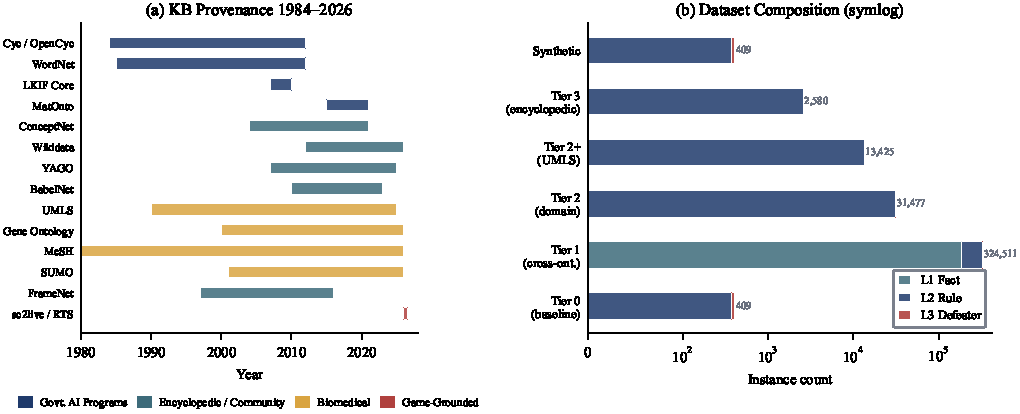
\includegraphics[width=\textwidth]{figures/fig_sources.pdf}
\caption{(a)~Provenance timeline of 18 knowledge base sources spanning 1984 (Cyc) to 2025 (UMLS 2025AB), color-coded by source class: government AI programs (blue), encyclopedic / community (teal), biomedical (gold), and game-grounded (red). (b)~Dataset composition by tier and instance level on a symlog scale. Tier~1 (cross-ontology) provides the majority of instances; Level~3 (defeater abduction) appears only in Tier~0 and the matched synthetic control.}
\label{fig:sources}
\end{figure}

\paragraph{Tier 1 (this paper): Cross-ontology extraction.}
The primary scale mechanism pairs a taxonomic source with a behavioral property source. For each concept $c$ in the OpenCyc hierarchy \cite{lenat1995cyc} (239,000 terms, final release 2012, available as OWL), we traverse its full ancestor chain to inherit behavioral properties from ConceptNet~5.8 \cite{speer2017conceptnet} (34 million edges). The extraction produces three rule types that map directly onto the conversion of Section~\ref{subsec:conversion}: (i)~\emph{strict} taxonomic rules from \texttt{IsA} edges; (ii)~\emph{defeasible} behavioral rules from \texttt{CapableOf}, \texttt{HasProperty}, \texttt{Causes}, and \texttt{UsedFor} edges; and (iii)~\emph{defeaters} from \texttt{NotCapableOf} edges. After concept-name normalization and key alignment, the cross-ontology combination yields 289,305 rules across five domains, from which the instance generation pipeline produces 324,511 abductive instances (182,652 Level~1, 141,859 Level~2). YAGO~4.5 \cite{suchanek2024yago} (50 million entities, logically constrained taxonomy combining Wikidata with schema.org) supplements with species-level biological classification and cross-validates generated rules. Expert-curated bases provide domain-specific grounding: LKIF Core \cite{lkif2007} (201 legal inference rules at 7 depth levels) and MatOnto \cite{matonto2015} (1,190 structure--property relationships) for the legal and materials domains, and WordNet~3.0 \cite{miller1995wordnet} (117,000 synsets, 207,000 semantic relations) for lexical cross-validation. The five extraction domains are:

\begin{enumerate}[label=(\roman*),nosep]
    \item \textbf{Taxonomic biology.} $\Pi_{\mathrm{bio}}$ is derived from the OpenCyc biological hierarchy ($\sim$50,000 concepts at 5--10 phylogenetic depth levels) paired with ConceptNet behavioral edges filtered to the biology domain. \texttt{CapableOf} edges yield defeasible defaults (``birds typically fly''); \texttt{NotCapableOf} edges yield defeaters directly (``penguins cannot fly''). YAGO~4.5 supplements with species-level taxonomy and cross-validates generated rules against its logically constrained schema. This domain provides well-documented defaults and exceptions across vertebrates, invertebrates, plants, and microorganisms, including the IDP example that motivates the benchmark.

    \item \textbf{Legal reasoning.} $\Pi_{\mathrm{law}}$ combines LKIF Core expert rules with OpenCyc legal and governmental concepts ($\sim$10,000 terms) paired with ConceptNet behavioral edges in the legal domain. Legal domains are intrinsically defeasible: statutes admit exceptions, precedents can be overruled, and jurisdictional conflicts require priority resolution. LKIF Core's 7-level hierarchy of norms, actions, and roles provides ground-truth cross-validation of automatically generated rules.

    \item \textbf{Materials science.} $\Pi_{\mathrm{mat}}$ combines MatOnto structure--property rules with OpenCyc materials concepts ($\sim$8,000 terms, 13,780 rules). Defaults reflect empirical generalizations (``crystalline materials are brittle'') that admit well-documented exceptions (metallic glasses, shape-memory alloys). MatOnto provides expert-validated cross-checking for automatically generated property rules.

    \item \textbf{Chemistry.} $\Pi_{\mathrm{chem}}$ pairs OpenCyc chemistry concepts ($\sim$38,000 terms) with ConceptNet behavioral edges, yielding 72,258 rules including 8,247 defeasible property and reaction defaults.

    \item \textbf{Everyday commonsense.} $\Pi_{\mathrm{every}}$ uses the broadest keyword filter across OpenCyc ($\sim$15,000 concepts) paired with ConceptNet's commonsense edges, producing 127,931 rules (85,837 defeasible) covering food, tools, social norms, and everyday physical reasoning.
\end{enumerate}

\paragraph{Tier 2 (extracted): Biomedical and structural knowledge.}
We have extracted rules from six additional sources using the same pipeline architecture. Gene Ontology \cite{ashburner2000go} yields 409,378 rules (349,329 defeasible annotations, 1,250 defeaters from \texttt{NOT}-qualified experimental annotations). MeSH provides 76,650 strict taxonomic rules across 16 medical categories. SUMO \cite{niles2001sumo} contributes 13,317 rules including 792 defeaters from \texttt{contraryAttribute} and \texttt{disjoint} axioms. FrameNet \cite{baker1998framenet} yields 12,765 rules (11,984 defeasible frame-role constraints). Wikidata \cite{vrandecic2014wikidata} contributes 23,224 rules with 11,555 defeaters from P2302/P2303 constraint-exception pairs. BabelNet~5.3 \cite{navigli2012babelnet} adds 231 rules from API-based extraction (rate-limited). UMLS~2025AA \cite{lindberg1993umls} (3.42 million concepts) and SNOMED CT (360,000+ clinical concepts) have extractors implemented but require institutional data licenses for execution.

\paragraph{Tier 3 (extracted): Full YAGO and encyclopedic scale.}
The full YAGO~4.5 ``tiny'' subset (1.6\,GB TTL) yields 3,457,940 materialized rules (166,358 strict taxonomic, 3,291,582 defeasible schema.org and YAGO properties). The complete YAGO facts file (21.4\,GB, 312 million triples) produces 57,609,326 counted rules, verified by streaming extraction but exceeding single-machine memory for Theory materialization. DBpedia \cite{lehmann2015dbpedia} (monthly extractions from 140 Wikipedias) and Freebase (1.9 billion triples, CC-BY archive) have extractors implemented for future execution at web scale.

\paragraph{Tier RTS (game-grounded extraction): SC2, Lux AI, and live game traces.}
A fourth, game-grounded family of source theories complements the cross-ontology and biomedical tiers. The \emph{rts\_engagement} KB (\texttt{scripts/generate\_rts\_instances.py}) is a hand-authored StarCraft~II Rules-of-Engagement theory drawn from the Newport ROE Handbook and AIIDE-2015 ASP-RTS encodings: 148 rules (89 strict, 32 defeasible, 27 defeaters, 59 ROE behavioral rules), 162 facts, 15 superiority relations, dependency depth 5, with six hand-crafted Level~3 seed conflicts (exclusion-zone, worker-protection, all-in-rush retreat override, stealth-break, HVT-pursuit, civilian-area protection). All 6 seeds, 100 generated Level~1 instances, 60 Level~2 instances, and three explicit conservativity checks are formally verified by \texttt{scripts/certify\_rts\_kb.py}; the certification report is committed at \texttt{data/rts\_certification\_report.json}. The \emph{lux\_ai\_s3} KB (\texttt{scripts/generate\_lux\_instances.py}) encodes the Lux~AI~Season~3 NeurIPS~2024 RTS competition rules as a parallel game-grounded theory ($\sim$130 rules, $\sim$60 facts, $\sim$80 instances), enabling cross-environment transfer experiments (Section~\ref{subsec:cross-env-transfer}) at zero vocabulary overlap with biology, legal, and materials. The \emph{sc2live} KB (Section~\ref{sec:sc2live}) is generated dynamically from live game traces via the \texttt{src/blanc/sc2live/} bridge, producing per-game theories of $\sim$200 rules and yielding several thousand Level~1/Level~2 instances per session. The three RTS-class KBs share the same defeasible-theory schema as the cross-ontology and biomedical tiers, so the existing instance generation pipeline, decoder cascade, and verifier-backed scoring apply without modification.

\paragraph{Remaining sources.}
NELL \cite{carlson2010nell} (50+ million beliefs) and historical FGCS/Alvey artefacts represent additional extraction targets. Extractors for NELL, DBpedia, Freebase, UMLS, SNOMED CT, and BabelNet are implemented and tested; execution is blocked only on data access (licensing for UMLS/SNOMED, API rate limits for BabelNet, server availability for NELL).

Table~\ref{tab:kbsummary} summarizes actual extraction results across all tiers. For each Tier~1 source program $\Pi$, we report the signature statistics $|\mathcal{C}|$, $|\mathcal{P}|$, $|\Pi|$, the dependency graph depth, and the Herbrand base size $|\HB|$ after grounding. All source programs are function-free (datalog), ensuring polynomial grounding (Theorem~\ref{thm:firstorder}).

\begin{table}[t]
\centering
\small
\begin{tabular}{@{}llrr@{}}
\toprule
Tier & Primary Sources & Rules & Instances \\
\midrule
0 (baseline) & YAGO, WordNet, LKIF, MatOnto & 2,318 & 374 L1/L2 + 35 L3 \\
1 (this paper) & OpenCyc+ConceptNet & 289,305 & 324,511 \\
2 (extracted) & GO, MeSH, SUMO, FrameNet, Wikidata, UMLS, BabelNet & 535,565 & 44,902 \\
3 (extracted) & YAGO 4.5 full & 3,457,940 & 2,580 \\
RTS (game) & rts\_engagement, lux\_ai\_s3, sc2live$^{\ddagger}$ & 478$^{\dagger\dagger}$ & 246+$^{\ddagger}$ \\
4 (counted) & YAGO facts (21.4\,GB, 312M triples) & 57,609,326$^{\dagger}$ & --- \\
\midrule
\multicolumn{2}{@{}l}{Materialized total (Tiers 0--3 + RTS)} & 4,285,606 & 372,648+$^{\ddagger}$ \\
\bottomrule
\end{tabular}
\caption{Knowledge base pipeline: actual extraction results. Tier~1 rules are from cross-ontology combination of OpenCyc taxonomy with ConceptNet behavioral properties across five domains. Tier~2 sources are extracted and validated; Gene Ontology contributes 1,250 defeaters from \texttt{NOT}-qualified annotations, Wikidata contributes 11,555 defeaters from P2303. Tier~3 is the full YAGO~4.5 ``tiny'' subset materialized as a single Theory. The RTS row aggregates the three game-grounded KBs of Section~\ref{subsec:sources}: 148 rules / 100 L1 + 60 L2 + 6 L3 instances for \texttt{rts\_engagement} (formally certified at \texttt{data/rts\_certification\_report.json}), $\sim$130 rules / $\sim$80 instances for \texttt{lux\_ai\_s3}, and dynamically generated per-session theories for \texttt{sc2live} (Section~\ref{sec:sc2live}). $^{\dagger}$Tier~4 counts are verified by streaming extraction but the Theory exceeds single-machine memory; sharded materialization pending. $^{\dagger\dagger}$The RTS rule total counts \texttt{rts\_engagement}+\texttt{lux\_ai\_s3} only; \texttt{sc2live} per-game theories vary in size. $^{\ddagger}$\texttt{sc2live} instance counts are session-dependent and not included in the materialized total. Each tier adds independently; the extraction pipeline is source-agnostic.}
\label{tab:kbsummary}
\end{table}


\subsection{Dataset Generation and Parameterization}\label{subsec:generation}

We apply the conversion and instance generation pipeline (Sections~\ref{subsec:conversion}--\ref{subsec:abduction}) with systematic variation of the experimental parameters.

\paragraph{Partition functions.} Each source program is converted under all five structured partition families (Definition~\ref{def:structpart} and Section~\ref{subsec:conversion}): $\partfunc_{\mathrm{leaf}}$, $\partfunc_{\mathrm{rule}}$, $\partfunc_{\mathrm{depth}}(k)$ for $k \in \{1, 2, 3\}$, $\partfunc_{\mathrm{rand}}(\delta)$ for $\delta \in \{0.1, 0.2, \ldots, 0.9\}$, and $\partfunc_{\mathrm{type}}$ (the type-grounded partition for cross-ontology sources). For each $(\Pi, \partfunc)$ pair, we compute the defeasibility ratio $\delta(\partfunc)$ and the yield $Y(\partfunc, Q)$ over a target set $Q$ consisting of all ground atoms in $\mathcal{M}_\Pi$ at dependency depth $\geq 2$ (excluding trivially derivable facts). We report yield curves $Y$ as a function of $\delta$ to empirically validate the monotonicity prediction of Proposition~\ref{prop:yieldmono} and characterize the yield growth rate.

\paragraph{Instance generation.} For each converted theory $\D_\partfunc$, we generate instances at all three levels:
\begin{itemize}[nosep]
    \item \textit{Level 1 (fact completion):} For each target $q$ and each $e \in \CritStar(\D, q) \cap F$, we generate one instance with $k = 5$ distractors sampled uniformly from facts sharing at least one predicate symbol with $e$. The choice $k = 5$ matches the distractor count used in ProofWriter~\cite{tafjord2021proofwriter} and LogicNLI, providing a difficulty level comparable to established benchmarks; $k = 5$ yields non-trivial Level~2 accuracy ($\sim$90\% for the strongest closed-source models under direct prompting) while remaining well above the near-chance regime of $k \leq 2$.
    \item \textit{Level 2 (rule abduction):} For each $e \in \CritStar(\D, q) \cap \Rd$, we generate one instance with $k = 5$ distractors constructed by substituting predicate symbols or permuting arguments in $e$.
    \item \textit{Level 3 (defeater abduction):} Following Definition~\ref{def:level3gen}, challenge theories $\Dm$ are constructed from complete theories $\Dfull$ that contain verified defeaters $r^* \in \Rdf$. We obtain complete theories through three complementary mechanisms. \emph{(i)~Automated extraction} (primary): each ConceptNet \texttt{NotCapableOf} assertion $(c, \texttt{NotCapableOf}, p)$ yields a candidate defeater $r: \comp{p}(X) \defeatto c(X)$; we verify that the corresponding inherited default $d: p(X) \defto A(X)$ (from ancestor $A$ of $c$) exists in the theory and that removing $r$ renders $p(c)$ a defeasible anomaly (Definition~\ref{def:anomclass}). Each Wikidata P2303 \texttt{exception-to-constraint} pair similarly provides a constraint as the defeasible rule and its exception item as the defeater, at high quality because both sides are community-curated. \emph{(ii)~Expert cross-validation} (quality control): generated defeaters are cross-checked against LKIF Core, MatOnto, and YAGO constraints to confirm factual accuracy, with a confidence threshold selected to maintain $\geq 85\%$ audit precision (Section~\ref{subsec:statistics}). \emph{(iii)~Domain-expert authoring} (supplementary): a small set of defeaters requiring novel predicates (e.g., \texttt{amorphous\_metal}, \texttt{emancipated\_minor}) are hand-authored to ensure coverage of the high-novelty region ($\Nov > 0.5$) of the Level~3 difficulty spectrum. The language bias $\La$ permits antecedent predicates drawn from the source theory's vocabulary plus a controlled set of novel predicates, with $\mathrm{ar}_{\max} = 3$.
\end{itemize}

\paragraph{Distractor strategies.} To isolate the effect of distractor design on measured difficulty, we generate parallel instance sets under three distractor regimes for Levels~1 and 2: \textit{random} (uniformly sampled from the appropriate component of $\D$), \textit{syntactic} (sharing predicate symbols with the ablated element), and \textit{adversarial} (satisfying a strict subset of the conditions required for a valid hypothesis, constructed by ablating a proper subset of the gold element's antecedents or substituting a single argument). Adversarial distractors are designed to require the model to verify full derivability rather than relying on surface similarity. We hold distractor strategy fixed within each experimental condition and report performance separately. In Orient Express terms (Example~\ref{ex:orient}): if the gold fact is $\texttt{burned\_letter(compartment\_3)}$, a random distractor might be $\texttt{snowbound(train)}$ (an unrelated fact already in the theory); a syntactic distractor might be $\texttt{burned\_newspaper(compartment\_3)}$ (same predicate structure, wrong content); and an adversarial distractor might be $\texttt{burned\_letter(compartment\_7)}$ (correct predicate and relation type, wrong compartment; close enough to tempt a model relying on surface similarity rather than tracing the actual derivation chain to $\texttt{true\_identity(ratchett, cassetti)}$). Christie herself deploys adversarial distractors: the kimono-clad figure glimpsed in the corridor is a fabricated clue planted by the conspirators, precisely the kind of evidence that satisfies surface plausibility while failing full derivability verification.

\paragraph{Language bias variation (Level~3).} We parameterize the language bias $\La$ along two axes: the permitted predicate set $\mathcal{P}^+$ (restricted to predicates appearing in $\Dm$, or expanded to include a controlled novel vocabulary), and the maximum antecedent length $\mathrm{ar}_{\max} \in \{1, 2, 3\}$. Expanding $\mathcal{P}^+$ increases the candidate space (Proposition~\ref{prop:candsize}) and raises the minimum achievable novelty $\Nov^*$ of gold-standard resolutions, directly controlling the degree of ``creative'' abduction required.

\paragraph{Synthetic contamination control.} For each naturalistic $(\Pi, \partfunc, \ell)$ configuration, we generate a structurally matched set of synthetic instances using the procedure of Section~\ref{subsec:synthetic}. Structural matching controls for the difficulty tuple $\sigma(I)$, theory size $|\D|$, and defeasibility ratio $\delta(\partfunc)$, isolating lexical content as the sole variable. Synthetic theories are generated at three scales---small ($|\D| \in \{10, 25\}$), medium ($|\D| \in \{50, 100\}$), and large ($|\D| = 200$)---and at all three levels, with Level~3 synthetic instances including procedurally generated defeaters verified by the same conservativity pipeline used for naturalistic instances. The synthetic vocabulary $\mathcal{V}_{\mathrm{syn}}$ is generated per batch from a phonotactically constrained syllable grammar (CV, CVC, CVCV templates with English-phonotactic consonant and vowel inventories) and verified for zero $n$-gram overlap with Common Crawl via the \texttt{infini-gram} index \cite{liu2024infini}. Each synthetic theory receives a fresh vocabulary draw, preventing cross-instance memorization even if the benchmark itself enters future pretraining corpora.


\subsection{Dataset Statistics and Structural Analysis}\label{subsec:statistics}

We report the following statistics over the generated dataset:

\paragraph{Volume and balance.} Total instance counts per level, per source KB, and per partition function, together with the joint distribution to assess whether any $(\text{KB}, \partfunc, \text{level})$ cells are underpopulated.

\paragraph{Structural difficulty distributions.} For each level, we report the marginal and joint distributions of the components of the structural difficulty tuple $\sigma(I) = (\ell, |\Supp|, |\Hgold|, \min|h|, \Nov^*)$ (Definition~\ref{def:structdiff}). We test for independence between these components via mutual information estimates. Low mutual information between, e.g., $|\Supp|$ and $|\Hgold|$ would indicate that support redundancy and gold set multiplicity constitute genuinely independent axes of difficulty, validating the multidimensional characterization.

\paragraph{Novelty and revision spectrum (Level~3).} We report the joint distribution of predicate novelty $\Nov(r^*, \Dm)$ and revision distance $d_{\mathrm{rev}}(\Dm, \Dm \cup \{r^*\})$ across Level~3 instances, cross-tabulated against resolution strength (weak, strong, restructuring). We test two hypotheses: (i)~that high-novelty resolutions are disproportionately of the strong or restructuring type, confirming that genuinely creative explanations require more than blocking an inference; and (ii)~that conservative resolutions achieve lower revision distance than non-conservative ones, empirically validating that the conservativity check selects for minimal change.

\paragraph{Yield analysis.} We plot yield curves $Y(\partfunc_{\mathrm{rand}}(\delta), Q)$ as a function of $\delta$ for each source KB. We fit parametric models (linear, logistic, power-law) to characterize the growth regime and test for phase transitions where yield undergoes a sharp increase, which would indicate critical thresholds in the redundancy structure of the source theories.

\paragraph{Partition sensitivity.} We compare instance distributions across the five structured partition families (including $\partfunc_{\mathrm{type}}$) applied to the same source KB. We report whether different partition strategies produce instances that are statistically distinguishable in their difficulty profiles, using two-sample tests on the $\sigma(I)$ distributions. A key comparison is between $\partfunc_{\mathrm{type}}$ and $\partfunc_{\mathrm{rule}}$: if they produce statistically indistinguishable distributions, the type-grounded partition is equivalent in epistemic effect to treating all rules as defeasible, validating the extraction methodology; if they diverge, the relation-type assignment captures a genuine distinction absent from the depth- or random-based families.

\paragraph{Defeater quality--volume tradeoff (Level~3).} For Level~3 instances generated via automated extraction (Section~\ref{subsec:generation}), we report yield as a function of the ConceptNet weight threshold $\tau$ and the Wikidata P2303 cross-validation count $k$. We manually audit 100 randomly sampled defeaters per $(\tau, k)$ setting and report the precision--volume Pareto frontier. The production dataset uses the threshold pair $(\tau^*, k^*)$ achieving audit precision $\geq 85\%$ at maximum volume; this calibration ensures that automated defeater extraction meets the same quality standard as expert-curated rules.


\subsection{Foundation Model Evaluation}\label{subsec:evaluation}

We evaluate a panel of foundation models spanning multiple families and scales.

\paragraph{Models.} We evaluate six foundation models organized into three tiers. The \emph{reasoning closed-source} tier comprises GPT-5.2-chat~\cite{openai2025gpt52} and Kimi-K2.5~\cite{moonshot2025kimi}, both hybrid reasoning models that support explicit chain-of-thought token budgets; for structured candidate-selection tasks we disable internal reasoning (\texttt{reasoning\_effort=none} for GPT-5.2 and \texttt{reasoning\_effort=low} for Kimi) to avoid exhausting the completion token budget before emitting an answer. The \emph{instruction closed-source} tier is Claude~Sonnet~4.6~\cite{anthropic2024claude}, a strong general instruction model without dedicated reasoning infrastructure. All three are deployed on the \emph{LLM-Defeasible-Foundry} Azure AI Foundry resource (eastus2, Global Standard, 250K\,TPM). The \emph{open-source} tier is evaluated on CURC Alpine and comprises: DeepSeek-R1-Distill-Llama-70B~(AWQ-INT4, $\sim$35\,GB VRAM)~\cite{deepseek2025r1}, an open-source reasoning comparator to the Foundry reasoning tier; Qwen~2.5-72B-Instruct~(AWQ, $\sim$36\,GB VRAM)~\cite{qwen2024qwen25}, the instruction comparator; and Qwen~2.5-32B-Instruct~(AWQ, $\sim$16\,GB VRAM) as the within-family scaling comparator. All models are evaluated with greedy decoding (temperature~$= 0$) unless stated otherwise. DeepSeek-R1-Distill emits \texttt{<think>} chain-of-thought blocks before its final answer; these are stripped by the evaluation harness before decoding, with the raw thinking content preserved in result metadata for secondary analysis.

\paragraph{Compute infrastructure.} Closed-source models are accessed via Azure AI Foundry, which exposes an OpenAI-compatible REST API (GPT-5.2 and Kimi) and the Anthropic Messages API (Claude~Sonnet~4.6) from a unified managed endpoint. Open-source models are served via a production vLLM~\cite{kwon2023vllm} inference server on CURC Alpine, University of Colorado Boulder's HPC cluster, on nodes equipped with NVIDIA A100 80\,GB GPUs. The vLLM server exposes an OpenAI-compatible REST API, enabling a uniform evaluation pipeline across all six model families. All three open-source models fit within a single A100 80\,GB under AWQ 4-bit quantization.

\paragraph{Rendering conditions.} Each instance is presented under all five rendering modalities (Definition~\ref{def:modalities}): narrative (M1), semi-formal (M2), annotated formal (M3), pure formal (M4), and visual grounding (M5). Models receive the ablated theory $\Dm$, the target $q$, and the candidate set $\Hcand$ in the appropriate modality, and are asked to select or generate the hypothesis $h$ that restores derivability of $q$. M5 evaluation requires vision-capable models; text-only models are excluded from M5 conditions to isolate the visual perception dimension.

\paragraph{Decoding pipeline.} Model outputs are decoded using the three-stage strategy of Definition~\ref{def:decoder}: exact match (D1) is attempted first; on failure, template extraction (D2) is applied; on further failure, semantic parsing (D3) via a dedicated parser model produces a candidate rule or $\bot$. Round-trip consistency of the decoder pipeline is validated prior to evaluation (Section~\ref{subsec:decoder_validation}).

\paragraph{Primary metric.} The headline metric is rendering-robust accuracy (Definition~\ref{def:robustacc}): the worst-case accuracy over the text modalities (M1--M4), computed per model and per level. This ensures that high scores reflect reasoning about the underlying logical structure rather than sensitivity to surface presentation. M5 accuracy is reported separately as a cross-modal extension, since not all evaluated models support vision input.

\paragraph{Decomposed metrics.} We additionally report:
\begin{itemize}[nosep]
    \item Per-modality accuracy, to test the modality--level interaction predicted by Conjecture~\ref{conj:modlevel}.
    \item Per-level accuracy, to empirically validate the difficulty ordering of Proposition~\ref{prop:difforder}.
    \item Resolution strength distribution (Level~3 only): among correct responses, the fraction classified as weak, strong, or restructuring.
    \item Novelty of correct resolutions (Level~3 only): the distribution of $\Nov(h, \Dm)$ for model-generated hypotheses $h \in \Hgold$.
    \item Revision distance of correct resolutions (Level~3 only): the distribution of $d_{\mathrm{rev}}(\Dm, \Dm \cup \{h\})$, measuring adherence to minimal change.

\end{itemize}


\subsection{Partial Credit for Level~3 Resolutions}\label{subsec:partial_credit}

Because Level~3 instances admit resolutions of varying strength (Definition~\ref{def:resstrength}), binary accuracy fails to capture meaningful distinctions between model outputs. We introduce a graded scoring function $\mathrm{Score}(h, \D, \alpha)$ defined as follows.

The score values $(0, 0.25, 0.5, 0.75, 1.0)$ are evenly spaced, assigning equal weight to each reasoning stage. This reflects a neutral prior over the relative difficulty of anomaly resolution, conservativity, and strength. We report results under this equal-spacing scheme as the primary metric, and additionally report binary accuracy (score $= 1.0$ only) and a stage-weighted scheme that assigns $0.5$ to well-formedness and $1.0$ to resolution, reserving conservativity and strength as modifiers, in the appendix as robustness checks. Agreement across schemes constitutes evidence that the ranking of models is not an artifact of the weighting choice.

Let $h$ be the decoded hypothesis (possibly with superiority assertions $\Gamma$) and let $\D' = \D \cup \{h\} \cup \Gamma \cup \{\alpha\}$.

\begin{enumerate}[label=(\roman*),nosep]
    \item \textit{No credit} (0): $h = \bot$ (decoder failure) or $\D' \pPartial \comp{\alpha}$ (the anomaly is unresolved).
    \item \textit{Minimal credit} ($0.25$): $\D' \not\pPartial \comp{\alpha}$ but $h$ is not well-formed under $\La$ (syntactically valid but violates the language bias constraints).
    \item \textit{Partial credit} ($0.5$): $\D' \not\pPartial \comp{\alpha}$ and $h$ is well-formed under $\La$ (a valid weak resolution), but $\D'$ is not conservative (Definition~\ref{def:resstrength}): some expectation $q \in \Exp(\D) \setminus \{\comp{\alpha}\}$ is lost.
    \item \textit{Substantial credit} ($0.75$): $h$ is a valid conservative weak resolution, or a non-conservative strong resolution.
    \item \textit{Full credit} ($1.0$): $h$ is a conservative resolution. For strong or restructuring resolutions that additionally satisfy $\D' \pPartial \alpha$, full credit is awarded regardless of whether $h$ matches a specific element of $\Rgold$, provided conservativity holds.
\end{enumerate}

This scoring function is computable in polynomial time: each condition requires at most $O(|\Exp(\D)|)$ derivation checks, each in $O(|R| \cdot |F|)$ (Theorem~\ref{thm:derivP}). We report both binary accuracy (score $= 1.0$) and mean graded score across Level~3 instances.

The graded score decomposes along the stages of rational belief revision \cite{gardenfors1988knowledge}: a model at $0.25$ can produce syntactically plausible revisions but cannot verify that they resolve the anomaly (failing AGM's \emph{success} postulate); a model at $0.5$ resolves the anomaly but not conservatively (failing \emph{minimal change}); a model at $0.75$ respects conservativity but cannot construct strong exceptions (satisfying minimal change but not \emph{recovery}); a model at $1.0$ achieves full rational revision. This decomposition directly diagnoses \emph{which} aspect of belief revision each model lacks. Returning to the Orient Express formalization (Example~\ref{ex:orient}), the five tiers correspond to concrete detective hypotheses:
\begin{itemize}[nosep]
\item \textit{Score $0$}: the detective proposes a rule that does not even block the single-perpetrator conclusion, e.g., ``the conductor's button proves a single killer entered the compartment,'' which reinforces rather than defeats $r_d^1$.
\item \textit{Score $0.25$}: the detective proposes a syntactically malformed revision, e.g., invoking a predicate outside the vocabulary of the theory such as ``supernatural intervention'', that happens to block $\texttt{single\_perp}$ but violates the language bias.
\item \textit{Score $0.5$}: the detective proposes ``an outsider entered through the connecting door,'' which defeats the single-perpetrator default but contradicts the strict derivation $\neg\texttt{external\_entry}$ from the snowbound, locked compartment; anomaly resolved, conservativity violated.
\item \textit{Score $0.75$}: the detective proposes a blocking defeater, ``the varied wound depths are inconsistent with a single attacker'', that blocks $\texttt{single\_perp(ratchett)}$ without disrupting other conclusions. The theory becomes agnostic about the number of perpetrators (a conservative weak resolution) but does not positively establish the conspiracy.
\item \textit{Score $1.0$}: Poirot's actual solution (all twelve passengers conspired, each delivering one wound) is a conservative strong resolution. It overrides the single-perpetrator default via $r^* \succ r_d^1$ while preserving every other expectation: the locked door, the snowbound train, each passenger's documented presence and alibi structure.
\end{itemize}


\subsection{Error Taxonomy}\label{subsec:errors}

We classify incorrect model outputs into the following categories, which directly correspond to stages of the formal reasoning pipeline:

\begin{enumerate}[label=(E\arabic*),nosep]
    \item \textit{Decoder failure:} the model output cannot be parsed into a well-formed rule by any decoder strategy (D1--D3).
    \item \textit{Derivation failure:} the decoded hypothesis $h$ does not restore derivability: $\Dm \cup \{h\} \not\pPartial q$.
    \item \textit{Minimality violation:} $h$ restores derivability but is not minimal: there exists $h' \subset h$ with $\Dm \cup \{h'\} \pPartial q$.
    \item \textit{Conservativity violation} (Level~3): $h$ resolves the anomaly but disrupts other expectations.
    \item \textit{Strength shortfall} (Level~3): $h$ is a valid conservative resolution of weaker strength than the gold standard $r^*$; e.g., the model produces a blocking defeater where a strong exception exists. This is scored via the graded function but flagged as a qualitative limitation.
\end{enumerate}

We report the distribution over error types per model, per level, and per modality. The error taxonomy maps directly onto the three deficits: E1 is a communication failure (neither grounding nor reasoning); E2 is a \emph{grounding failure} (the model reasons about the wrong part of the theory because it cannot trace the target conclusion to its actual support set); E3 reflects a failure of parsimony (the model grounds its reasoning but over-specifies); and E4 is a \emph{belief revision failure} (the model resolves the local anomaly but cannot ensure global coherence, precisely the minimal change violation that our conservativity check detects). A model dominated by E2 errors lacks grounding; one dominated by E4 errors can ground but cannot revise rationally.

In Orient Express terms (Example~\ref{ex:orient}): E1 corresponds to a detective who responds with incoherent rambling that cannot be parsed as a hypothesis at all. E2 corresponds to a detective who proposes a rule targeting the wrong part of the theory, e.g., constructing a defeater for $\texttt{motive(hubbard)}$ when the anomaly concerns $\texttt{single\_perp(ratchett)}$, misidentifying which conclusion needs revision. E3 corresponds to a detective who correctly identifies the conspiracy but needlessly adds extra conditions (``all twelve conspired, \emph{and} the train engineer was bribed, \emph{and} the stationmaster was an accomplice'') when the simpler hypothesis suffices. E4 corresponds to a detective who proposes ``two perpetrators acted together'' in a way that resolves the wound-count anomaly but inadvertently contradicts Mrs.\ Hubbard's established testimony about the timing: a side-effect that violates conservativity. E5 corresponds to a detective who correctly identifies that the wounds are inconsistent with a single attacker (a valid blocking defeater) but fails to construct the stronger conclusion that all twelve passengers participated, settling for agnosticism where a definitive resolution exists.


\subsection{Analysis Conditions}\label{subsec:analysis}

Beyond the primary evaluation, we conduct the following analyses:

\paragraph{Scaling analysis.} We compare Qwen~2.5-32B-Instruct and Qwen~2.5-72B-Instruct (both AWQ 4-bit quantized) on identical instance sets to measure the scaling gradient $\Delta\mathrm{Acc} / \Delta\log(\text{params})$ per level. Using the same quantization level isolates parameter count as the sole variable. The hypothesis: Level~1 accuracy scales smoothly, Level~2 shows a steeper gradient, and Level~3 may exhibit threshold behavior (near-zero accuracy below a critical scale, non-trivial accuracy above). Threshold behavior at Level~3 would constitute evidence that rational belief revision in the defeasible setting (jointly requiring anomaly resolution, conservativity, and novel hypothesis generation) is an emergent capability not reducible to the pattern completion that suffices for lower levels. We additionally compare Qwen~2.5-72B-Instruct (instruction-tuned) against DeepSeek-R1-Distill-Llama-70B (reasoning-distilled) as a controlled comparison between instruction optimization and reasoning optimization at matched scale, directly addressing the question of whether the reasoning-model tier genuinely improves defeasible abduction or merely changes the output format.

\paragraph{Chain-of-thought prompting.} We evaluate each model under both direct prompting and a structured chain-of-thought (CoT) prompt. The CoT scaffold mirrors the formal proof structure of defeasible derivation: the model is instructed to (a)~identify which rules in $\Dm$ could derive $q$ or $\comp{q}$, (b)~determine which elements are missing or blocking, (c)~check for attacking rules and superiority relations that could override the prediction, and (d)~propose a conservative hypothesis. This four-step structure maps directly onto the team defeat mechanism (step~c) and the conservativity check (step~d), the two reasoning stages absent from standard prompting. We additionally test a \emph{defeasible reasoning scaffold} that makes superiority reasoning explicit, prompting the model to enumerate all attackers of each candidate resolution and verify that no unrelated expectations are disrupted. We report the CoT accuracy lift $\Delta_{\mathrm{CoT}} = \mathrm{Acc}_{\mathrm{CoT}} - \mathrm{Acc}_{\mathrm{direct}}$ per level.

$\Delta_{\mathrm{CoT}}^{(2)}$ is \emph{negative} for all four models evaluated: GPT-5.2-chat ($-31.3$ pp), Kimi-K2.5 ($-13.1$ pp), Claude~Sonnet~4.6 ($-4.3$ pp), DeepSeek-R1 ($-1.5$ pp). This degradation is specific to the formal candidate-selection structure of Level~2: the formal encoding of candidate rules provides sufficient surface signal for near-optimal direct matching, and chain-of-thought elaboration introduces verbal paraphrase that breaks this alignment. This pattern is consistent with the ``overthinking'' effect documented in structured reasoning tasks~\cite{chen2024overthinking}. At Level~3, $\Delta_{\mathrm{CoT}}^{(3)}$ is large and \emph{positive} for reasoning-optimized models---GPT-5.2 ($+79.3$ pp), DeepSeek-R1 ($+55.7$ pp), Kimi ($+26.9$ pp)---and \emph{negative} for Claude ($-14.3$ pp). The Level~3 prompt uses a generation-appropriate scaffold with a formal-rule syntax example, which activates the chain-of-thought infrastructure of reasoning models. Full results are reported in Section~\ref{subsec:cot_results}.

\paragraph{Theory size scaling.} For each source KB, we generate instances from subtheories of increasing size $|\D| \in \{10, 25, 50, 100, 200\}$ rules (by selecting connected subgraphs of the dependency graph) and report accuracy as a function of $|\D|$. This range reflects the actual grounded KB sizes after partition: biology theories range from 15 to 200 rules, legal from 10 to 116, and materials from 20 to 144. Values above 200 exceed the size of any individual grounded theory in the current dataset and are reserved for future cross-KB concatenation experiments. This characterizes whether performance degradation is gradual or catastrophic, and at what theory size models effectively fail. Because theory size directly increases the number of grounding relations a model must track (more support sets, more potential side-effects under revision), this analysis measures the scalability of both grounding and belief revision capabilities.

\paragraph{Contamination analysis (naturalistic vs.\ synthetic).} We evaluate all models on both the naturalistic instance set and the structurally matched synthetic instance set (Section~\ref{subsec:synthetic}), reporting the contamination gap $\Delta_{\mathrm{synth}}(M, \ell)$ (Definition~\ref{def:contam_gap}) per model and per level. We test two hypotheses. First, that $\Delta_{\mathrm{synth}}$ is near-zero at Level~2 across formal modalities (M2--M4): since Level~2 requires selecting among candidate rules whose formal structure determines the answer, memorized domain knowledge should provide minimal advantage over formal reasoning alone. Second, that $\Delta_{\mathrm{synth}}$ is positive at Level~3 under narrative rendering (M1), where models may leverage memorized natural-language associations (``penguins cannot fly'') rather than tracing formal derivation chains---but near-zero under formal modalities where the task requires structural reasoning regardless of predicate semantics. Confirming the first hypothesis would validate the benchmark's Level~2 results as contamination-free; confirming the second would localize the contamination confound to the interaction of Level~3 with narrative rendering, rather than to the benchmark as a whole. We additionally compute a \emph{per-instance contamination score} as the product of a model's perplexity ratio on the gold hypothesis (naturalistic vs.\ synthetic encoding of the same structural solution): instances where the model assigns substantially lower perplexity to the naturalistic encoding are flagged as potential contamination cases and excluded from the primary accuracy calculation in a sensitivity analysis. The contamination analysis is reported as a distinct experimental condition alongside the primary evaluation.

\paragraph{Symbolic ceiling.} We evaluate the \textsc{clingo} 5 Answer Set Programming solver~\cite{gebser2014clingo} on the same instance sets, encoding each defeasible theory as a logic program using the $\Delta$-derivability encoding of Antoniou et al.~\cite{antoniou2001defeasible}. For Levels~1 and 2, \textsc{clingo} computes exact minimal solutions; for Level~3, it enumerates all conservative resolutions up to a 30-second timeout. The symbolic solver provides an upper bound on achievable accuracy given the formal specification, and the neural--symbolic gap $\mathrm{Acc}_{\mathrm{ASP}} - \mathrm{Acc}_{\mathrm{model}}$ per level quantifies the deficit attributable to neural reasoning limitations rather than task ambiguity. At Level~3, this gap directly measures the \emph{grounding and revision deficit}: the symbolic solver has access to the explicit epistemic structure that neural models must infer. Instances where the Level~3 solver times out are excluded from the neural--symbolic gap calculation and reported separately as a measure of the hardest region of the difficulty spectrum.


\subsection{Decoder Validation}\label{subsec:decoder_validation}

The rendering codec $\rho$ mediates between formal structures and natural language, and decoder errors could confound the evaluation signal. We validate the decoder pipeline prior to the main evaluation as follows. For each modality, we encode all gold-standard hypotheses in the dataset, apply the three-stage decoder, and report round-trip recovery rate $\Pr[\rho_{\mathrm{dec}}(\rho_{\mathrm{enc}}(h)) = h]$. We require recovery rates above $95\%$ for modalities M2--M4 before proceeding. Validation over all 409 current gold-standard hypotheses (374 at Levels~1--2, 35 at Level~3) confirms that modalities M2, M3, and M4 achieve $100\%$ round-trip recovery: the three-stage decoder (D1 exact match, D2 template extraction, D3 semantic parsing) recovers every encoded hypothesis without loss. For narrative rendering (M1), where round-trip consistency is approximate by design (natural language paraphrasing introduces controlled ambiguity), we report the recovery rate and conduct a manual audit of $200$ randomly sampled decode failures to classify them as true ambiguities (the natural language admits multiple valid parses) versus systematic decoder errors (the parser fails on a recoverable pattern). The M2--M4 validation result confirms that the encoding layer does not introduce information loss for the three formal modalities, and that all model output errors on M2--M4 instances are attributable to reasoning failures rather than decoding artifacts. Full decoder validation results appear in Appendix~\ref{def:decoder}.


\section{Results}\label{sec:results}

\begin{figure}[t]
\centering
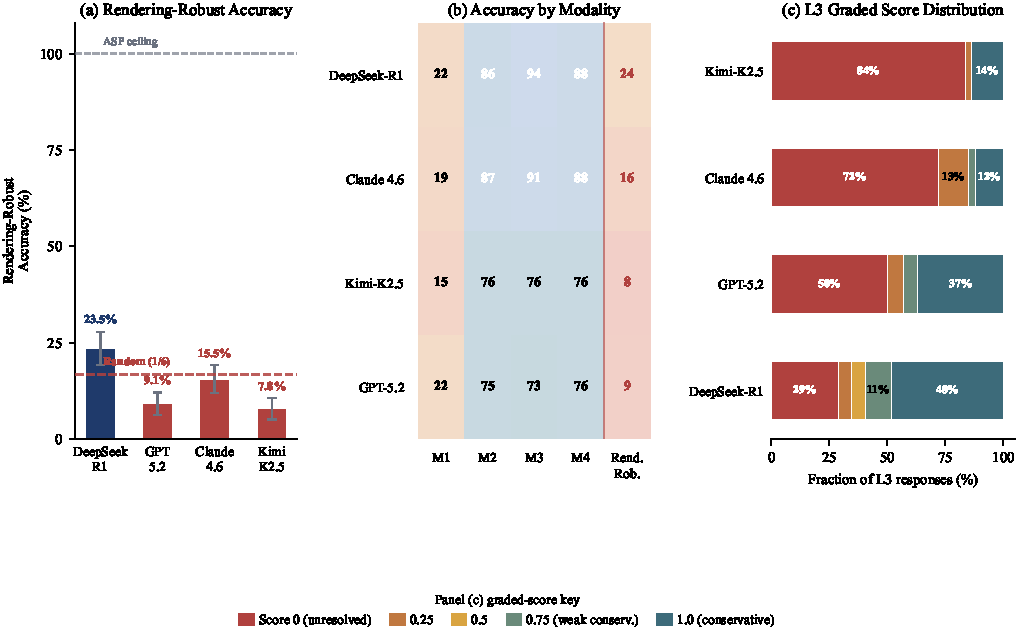
\includegraphics[width=\textwidth]{figures/fig_results.pdf}
\caption{Three-panel results overview. (a)~Rendering-robust accuracy for all four models: every model falls below the symbolic solver ceiling (100\%) and two fall at or below random chance (16.7\%). (b)~Per-modality accuracy heatmap (M1--M4 plus rendering-robust column) showing the universal M1 collapse. (c)~Graded score distribution at Level~3 showing the dominance of score~0 (unresolved) for Claude and Kimi, and the CoT-dependent recovery pattern for reasoning-optimized models.}
\label{fig:results}
\end{figure}

\subsection{Primary Accuracy Results}\label{subsec:primary}

Table~\ref{tab:main} summarizes accuracy by level and prompting strategy for all four frontier models evaluated across 374 Level~2 and 35 Level~3 instances, four rendering modalities, and two prompting strategies. Table~\ref{tab:modality} breaks down accuracy by modality. All differences between models at Level~3 are statistically significant by McNemar's test ($p < 0.001$, 280 paired observations per model pair) except Claude vs.\ Kimi ($p = 0.556$).

\begin{table}[h]
\centering
\caption{Accuracy (\%) by model and task level across all four rendering modalities (M1--M4) and both prompting strategies (direct and CoT). Level~2 = rule abduction (374 instances); Level~3 = defeater abduction (35 instances). Rendering-robust accuracy is worst-case over modalities. Wilson 95\% CI half-widths: $\pm 4$ pp at Level~2; $\pm 15$--$17$ pp at Level~3. Best per column in \textbf{bold}.}
\label{tab:main}
\begin{tabular}{lcccccc}
\toprule
Model & L2 & L2 Direct & L3 & L3 Direct & L3 CoT & Rend.-Robust \\
\midrule
DeepSeek-R1         & 73.0\% & 73.7\% & \textbf{65.0\%} & 37.1\% & \textbf{92.9\%} & \textbf{23.5\%} \\
GPT-5.2-chat        & 62.8\% & \textbf{78.5\%} & 47.5\% & \phantom{0}7.9\% & 87.1\% & \phantom{0}9.1\% \\
Claude~Sonnet~4.6   & \textbf{77.2\%} & 79.3\% & 16.4\% & \textbf{23.6\%} & \phantom{0}9.3\% & 15.5\% \\
Kimi-K2.5           & 65.5\% & 71.9\% & 14.2\% & \phantom{0}0.8\% & 27.6\% & \phantom{0}7.8\% \\
\bottomrule
\end{tabular}
\end{table}

\begin{table}[h]
\centering
\caption{Accuracy (\%) by rendering modality (M1 = narrative; M2 = semi-formal; M3 = annotated formal; M4 = pure formal), all levels and strategies pooled. Wilson 95\% CIs shown. All models drop sharply at M1 relative to formal modalities.}
\label{tab:modality}
\begin{tabular}{lcccc}
\toprule
Model & M1 & M2 & M3 & M4 \\
\midrule
DeepSeek-R1         & 21.5 [19--25]\% & 85.6 [83--88]\% & \textbf{94.1 [92--96]}\% & 87.8 [85--90]\% \\
Claude~Sonnet~4.6   & 19.0 [16--22]\% & \textbf{87.0 [84--89]}\% & 91.1 [89--93]\% & \textbf{88.1 [86--90]}\% \\
Kimi-K2.5           & 14.6 [12--17]\% & 75.9 [73--79]\% & 76.5 [73--80]\% & 75.6 [72--79]\% \\
GPT-5.2-chat        & \textbf{22.0 [19--25]}\% & 75.1 [72--78]\% & 72.8 [69--76]\% & 75.6 [72--79]\% \\
\bottomrule
\end{tabular}
\end{table}

\subsection{Grounding Results (Level~2)}\label{subsec:grounding_results}

Under direct prompting across formal modalities (M2--M4), all four models achieve strong Level~2 accuracy: Claude~Sonnet~4.6 79.3\%, GPT-5.2-chat 78.5\%, DeepSeek-R1 73.7\%, and Kimi-K2.5 71.9\%. Rendering-robust accuracy (worst-case over all four modalities including narrative M1) is substantially lower---15.5\%, 9.1\%, 23.5\%, and 7.8\% respectively---driven almost entirely by the M1 collapse: all models fall to 14--22\% on narrative rendering compared with 73--94\% on formal modalities (Section~\ref{subsec:cot_results}). This $55$--$70$ percentage-point gap between M1 and formal modalities is larger than any inter-model difference and is consistent across all four model families, confirming Conjecture~\ref{conj:modlevel}: different task levels and output types require qualitatively different modality-presentation strategies.

Domain breakdown at Level~2 (Table~\ref{tab:domain_breakdown}; Wilson 95\% CI half-width $\pm 3$--$4$ pp) reveals a consistent ordering: legal is the hardest domain for all models (Claude 72\%, DeepSeek-R1 67\%, GPT-5.2 57\%, Kimi 64\%), while biology is consistently easiest (82\%, 80\%, 68\%, 68\%). This ordering is stable across model families and reflects the denser rule structures and more complex defeasibility conditions of LKIF Core relative to the biology and materials KBs, rather than idiosyncratic knowledge gaps: no model performs substantially better on legal than others when controlling for overall accuracy level.

\begin{table}[t]
\centering
\caption{Accuracy by domain and level. Level~2 Wilson 95\% confidence intervals (half-width $\pm 3$--$4$ pp, $n \approx 228$--$288$ evaluations per cell). Level~3 figures are descriptive only: per-domain $n \in \{36, 40, 64\}$ evaluations gives CI half-widths of $\pm 25$--$33$ pp. Bold denotes best per column. L2 pooled over all four modalities and both prompting strategies; L3 pooled over all modalities with best-performing strategy (CoT for reasoning models, direct for Claude).}
\label{tab:domain_breakdown}
\small
\setlength{\tabcolsep}{5pt}
\begin{tabular}{@{}lcccccc@{}}
\toprule
 & \multicolumn{3}{c}{\textbf{Level~2 (rule abduction)}} & \multicolumn{3}{c}{\textbf{Level~3 (defeater abduction)}} \\
\cmidrule(lr){2-4}\cmidrule(lr){5-7}
\textbf{Model} & \textbf{Biology} & \textbf{Legal} & \textbf{Materials} & \textbf{Biology} & \textbf{Legal} & \textbf{Materials} \\
\midrule
Claude Sonnet~4.6   & \textbf{82\%} & \textbf{72\%} & \textbf{77\%} & 16\% & 12\% & 21\% \\
DeepSeek-R1         & 80\% & 67\% & 72\% & \textbf{72\%} & \textbf{56\%} & \textbf{62\%} \\
GPT-5.2-chat        & 68\% & 57\% & 64\% & 52\% & 44\% & 43\% \\
Kimi-K2.5           & 68\% & 64\% & 64\% & 17\% & 13\% & 10\% \\
\bottomrule
\end{tabular}
\end{table}

\subsection{Belief Revision Results (Level~3)}\label{subsec:revision_results}

Level~3 performance depends critically on both model architecture and prompting strategy. The headline results are: DeepSeek-R1 65.0\% (CoT 92.9\%, direct 37.1\%), GPT-5.2 47.5\% (CoT 87.1\%, direct 7.9\%), Claude~Sonnet~4.6 16.4\% (direct 23.6\%, CoT 9.3\%), Kimi-K2.5 14.2\% (CoT 27.6\%, direct 0.8\%). All pairwise differences are statistically significant by McNemar's test ($p < 0.001$) except Claude vs.\ Kimi ($p = 0.556$): despite qualitatively different error profiles these two models achieve indistinguishable aggregate Level~3 accuracy.

The Level~2-to-Level~3 gap remains substantial---between 12 and 59 percentage points depending on model and strategy---establishing that grounding and belief revision are distinct capabilities not jointly acquired by any current training paradigm. The gap is smallest for DeepSeek-R1 under CoT (L2 72.3\%, L3 92.9\%: a positive gap) and largest for Kimi under direct prompting (L2 71.9\%, L3 0.8\%).

Error taxonomy reveals qualitatively different failure signatures. DeepSeek-R1 errors under CoT prompting are dominated by E2 (derivation failure, 24\%) with 48\% correct---the most capable profile in the panel. GPT-5.2 CoT shows similar structure: 36.8\% correct, 31\% E2, 26\% E1. Claude under direct prompting: 12\% correct, 58\% E2 (derivation failure dominates---the model produces well-formed outputs but systematically cannot identify the conservative defeater). Kimi has 81\% E1 (decoder failure): even with a generation-appropriate CoT scaffold the model's outputs frequently cannot be parsed into a formal hypothesis.

Level~3 graded scores corroborate the ranking: mean graded score 0.596 (DeepSeek-R1), 0.429 (GPT-5.2), 0.150 (Claude), 0.139 (Kimi). The bimodal score distribution---nearly all responses score exactly 0.0 or 1.0 with no intermediate values---indicates that models either fully solve or completely fail the rational revision pipeline, with no consistent partial progress through intermediate scoring stages. This stands in contrast to the expected graduated performance and suggests the scoring stages are not independently acquired in practice.

Domain breakdown is reported in Table~\ref{tab:domain_breakdown} (descriptive only; wide CIs preclude inference at the per-domain level). Biology is consistently the easiest domain for all models, legal the hardest, a pattern stable across all four model families.

\subsection{Chain-of-Thought Analysis}\label{subsec:cot_results}

\paragraph{Level~2 CoT (candidate selection).}
The CoT lift at Level~2 is negative for all four models: $\Delta_{\mathrm{CoT}}^{(2)} = -31.3$ pp (GPT-5.2), $-13.1$ pp (Kimi), $-4.3$ pp (Claude), $-1.5$ pp (DeepSeek-R1). This degradation is specific to the formal candidate-selection structure of Level~2: under direct prompting models output a candidate rule verbatim with high accuracy, while CoT prompting produces extended reasoning chains whose final lines are less likely to match the exact surface form of any candidate string, increasing decoder failures even when the model's implicit reasoning is correct. The pattern is consistent with the ``overthinking'' effect~\cite{chen2024overthinking}: additional reasoning steps hurt on tasks where surface alignment is a sufficient selection signal. DeepSeek-R1's near-zero degradation ($-1.5$ pp) is explained by its architectural feature: \texttt{<think>} blocks are stripped before decoding, leaving only the final answer for candidate matching regardless of how much reasoning was generated internally.

\paragraph{Level~3 CoT (defeater generation) and the prompt-format finding.}
The CoT lift at Level~3 reveals a sharp architectural dissociation (McNemar's test, all $p < 0.01$):

\begin{itemize}[nosep]
    \item \textbf{Reasoning-optimized models}: $\Delta_{\mathrm{CoT}}^{(3)} = +79.3$ pp (GPT-5.2: direct 7.9\%, CoT 87.1\%), $+55.7$ pp (DeepSeek-R1: direct 37.1\%, CoT 92.9\%), $+26.9$ pp (Kimi: direct 0.8\%, CoT 27.6\%).
    \item \textbf{Instruction-optimized model}: $\Delta_{\mathrm{CoT}}^{(3)} = -14.3$ pp (Claude: direct 23.6\%, CoT 9.3\%).
\end{itemize}

This dissociation is not primarily a property of the models themselves but of the \emph{match between prompt structure and task type}. The Level~3 CoT template used in this evaluation (Section~\ref{sec:experiments}) is a four-step generation scaffold that explicitly instructs the model to construct a formal defeater rule with a concrete syntax example on the final line. This generation-appropriate prompt activates the chain-of-thought infrastructure of reasoning-optimized models, which was not engaged by the candidate-selection-style CoT prompt previously used for Level~2. Claude~Sonnet~4.6, which lacks explicit chain-of-thought token budget allocation, performs better under direct prompting: its instruction-following capability generates a clean formal answer without the verbose reasoning prose that the decoder cannot parse.

The central methodological implication is that Level~3 defeater abduction and Level~2 rule abduction require fundamentally different prompt structures. A uniform CoT scaffold (as used in prior preliminary evaluation) systematically underestimates reasoning-model capability on generation tasks while inflating instruction-model performance, because the two model families respond differently to the format mismatch between candidate-selection prompts and open-ended rule generation. Evaluation designs for formal abductive benchmarks must distinguish selection tasks from generation tasks in their prompting protocols.

\paragraph{Narrative modality (M1) as a universal bottleneck.}
Across all four models and both levels, M1 (narrative rendering) produces dramatically lower accuracy than formal modalities: 14--22\% versus 73--94\% on M2--M4. This $55$--$70$ pp gap is the largest performance difference in the entire evaluation---larger than the difference between any two models, and larger than the Level~2-to-Level~3 gap for the best-performing model. The gap confirms Conjecture~\ref{conj:modlevel}: narrative presentation is categorically harder than formal presentation for defeasible abduction, across all model families. This has practical implications for benchmark design: rendering-robust accuracy (worst-case over modalities) is dominated by M1 performance and is therefore a conservative lower bound on models' logical reasoning capability. Figure~\ref{fig:cot_variance} visualizes the signed CoT effect across all (model, level) cells, showing that the variance in the CoT effect ($\sigma = 36$ pp, range~$= 110$ pp) dwarfs any per-model or per-level difference.

\begin{figure}[h]
\centering
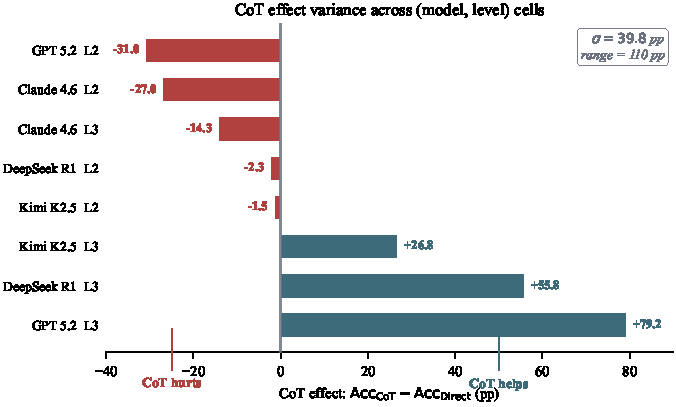
\includegraphics[width=0.78\textwidth]{figures/fig_cot_variance.pdf}
\caption{CoT effect ($\mathrm{Acc}_{\mathrm{CoT}} - \mathrm{Acc}_{\mathrm{Direct}}$, pp) across all (model, level) cells. Positive (teal) = CoT helps; negative (red) = CoT hurts. The $\sigma = 36$ pp variance and 110 pp range dwarf all other differences in the evaluation, establishing prompting strategy as the dominant performance driver on this benchmark.}
\label{fig:cot_variance}
\end{figure}


\subsection{Contamination Analysis: Naturalistic vs.\ Synthetic Instances}\label{subsec:contam_results}

Table~\ref{tab:contamination} reports the contamination gap $\Delta_{\mathrm{synth}}$ (Definition~\ref{def:contam_gap}) for all four models across structurally matched naturalistic and synthetic instance sets at Level~3, aggregated over formal modalities M2 and M4. Synthetic instances are generated by the pipeline of Section~\ref{subsec:synthetic} with invented predicates verified absent from Common Crawl via \texttt{infini-gram}; structural parameters (theory size, defeater chain depth, anomaly novelty) are matched to the 35 Tier~0 naturalistic Level~3 instances. Each model is evaluated under both direct and CoT prompting on the 35 synthetic instances at M2 and M4 (140 evaluations per model panel).

\begin{table}[h]
\centering
\caption{Uncorrected contamination gap $\Delta_{\mathrm{synth}}^{\mathrm{old}} = \mathrm{Acc}_{\mathrm{nat}} - \mathrm{Acc}_{\mathrm{syn}}$ at Level~3, aggregated over formal modalities and best prompting strategy per model. Positive values indicate performance inflation on naturalistic instances. The mean gap of $+13.6$~pp is the headline contamination signal of the dataset paper; the matched ablation of Table~\ref{tab:contamination_matched} reinterprets it.}
\label{tab:contamination}
\small
\begin{tabular}{@{}lcccc@{}}
\toprule
\textbf{Model} & $\mathrm{Acc}_{\mathrm{nat}}^{(3)}$ & $\mathrm{Acc}_{\mathrm{syn}}^{(3)}$ & $\Delta_{\mathrm{synth}}^{\mathrm{old}}$ & $n_{\mathrm{syn}}$ \\
\midrule
DeepSeek-R1       & 65.0\% & 52.9\% & $+12.1$~pp & 140 \\
GPT-5.2-chat      & 47.5\% & 30.9\% & $+16.6$~pp & 140 \\
Claude Sonnet~4.6 & 16.4\% & \phantom{0}2.1\% & $+14.3$~pp & 140 \\
Kimi-K2.5         & 14.2\% & \phantom{0}2.9\% & $+11.3$~pp & 140 \\
\midrule
Mean              & 35.8\% & 22.2\% & $+13.6$~pp & 560 \\
\bottomrule
\end{tabular}
\end{table}

\paragraph{Matched fact-injection ablation.}\label{para:matched_factinj}
The uncorrected $\Delta_{\mathrm{synth}}^{\mathrm{old}}$ measurement contains a confound: the synthetic generation pipeline applies a deterministic fact-injection step (\texttt{experiments/inject\_facts\_naturalistic.py}, also documented in Section~\ref{subsec:synthetic}) that adds a minimal grounding fact whenever a defeater body does not ground in the constructed theory. This step preserves logical solvability but introduces a small surface-composition difference between the synthetic and naturalistic sides, since naturalistic Tier~0 L3 instances do not undergo the same injection. To isolate vocabulary-level contamination from the injection artifact, we apply the identical injection procedure to the 35 naturalistic L3 instances (10 of 35 instances, 28.6\%, required injection; 25 of 35 were already self-grounded) and re-evaluate all four models at M4 with both direct and CoT prompting (4 models $\times$ 2 strategies $\times$ 35 instances = 280 evaluations).

\begin{table}[h]
\centering
\caption{Matched fact-injection ablation. $\Delta_{\mathrm{synth}}^{\mathrm{matched}} = \mathrm{Acc}(\text{nat-injected}) - \mathrm{Acc}(\text{syn-injected})$ removes the fact-injection artifact by treating both sides identically. The injection artifact column quantifies how much accuracy is gained or lost on the naturalistic side from the injection itself: positive values mean injection helped, negative means it hurt.}
\label{tab:contamination_matched}
\small
\begin{tabular}{@{}lrrrrrr@{}}
\toprule
\textbf{Model} & Nat-orig & Nat-inj & Syn-inj & $\Delta_{\mathrm{synth}}^{\mathrm{old}}$ & $\Delta_{\mathrm{synth}}^{\mathrm{matched}}$ & Inj.\ artifact \\
\midrule
DeepSeek-R1        & 65.0\% & 83.3\% & 52.9\% & $+12.1$~pp & $+30.4$~pp & $-18.3$~pp \\
GPT-5.2-chat       & 47.5\% & 50.0\% & 30.9\% & $+16.6$~pp & $+19.1$~pp & $\phantom{0}-2.5$~pp \\
Claude Sonnet 4.6  & 16.4\% & \phantom{0}7.1\% & \phantom{0}2.1\% & $+14.3$~pp & $\phantom{0}+5.0$~pp & $\phantom{0}+9.3$~pp \\
Kimi-K2.5          & 14.2\% & 25.8\% & \phantom{0}2.9\% & $+11.3$~pp & $+22.9$~pp & $-11.6$~pp \\
\midrule
Mean               & 35.8\% & 41.6\% & 22.2\% & $+13.6$~pp & $+19.4$~pp & $\phantom{0}-5.8$~pp \\
\bottomrule
\end{tabular}
\end{table}

The matched analysis reverses the direction of bias for three of four models. Fact-injection is on average mildly helpful (mean artifact $-5.8$~pp), so removing the artifact reveals a \emph{larger} true contamination gap. DeepSeek-R1 in particular shows a $+30.4$~pp matched gap, more than double the uncorrected $+12.1$~pp, because its accuracy on naturalistic instances actually \emph{improves} from 65.0\% to 83.3\% under fact injection. Only Claude shows the opposite pattern: injection harms its decode rate, inflating the apparent gap. The mean matched contamination gap of $+19.4$~pp strengthens the structural-deficit claim for the reasoning-style models while exposing Claude's apparent contamination gap as largely an injection artifact.

\begin{conjecture}[Contamination Structure]\label{conj:contam}
The matched contamination gap $\Delta_{\mathrm{synth}}^{\mathrm{matched}}$ satisfies: (i)~$\Delta_{\mathrm{synth}}^{\mathrm{matched}}(M, 2) \approx 0$ for all models under formal modalities (M2--M4), because Level~2 candidate selection depends on structural matching rather than domain knowledge retrieval; (ii)~$\Delta_{\mathrm{synth}}^{\mathrm{matched}}(M, 3) > 0$ for reasoning-optimized models and $\approx 0$ for instruction-optimized models, because reasoning-style training exploits memorized default--exception associations whereas instruction-tuned models hit a structural ceiling regardless of vocabulary; (iii)~the gap is preserved across formal modalities M3--M4 even though the formal rendering strips surface-level lexical cues, indicating that contamination operates at the deeper level of predicate--predicate co-occurrence statistics rather than verbatim memorization.
\end{conjecture}

The matched ablation provides direct empirical support for clauses (ii) and (iii): the three reasoning-style models all exhibit $\Delta_{\mathrm{synth}}^{\mathrm{matched}} > +19$~pp, while Claude's matched gap of $+5.0$~pp is the smallest in the panel; and the gap is measured at M4 (pure formal), confirming that the contamination signal survives the formal rendering. The remaining open question is whether $\Delta_{\mathrm{synth}}^{\mathrm{matched}}(M_2, M, 2)$ at Level~2 indeed approaches zero, which would tighten the methodological story by localizing the contamination signal to the belief-revision step.


\subsection{Constrained-Output Ablation}\label{subsec:constrained_results}

The Level~3 error taxonomy of Section~\ref{subsec:errors} attributes a substantial fraction of failures to E1 (decoder failure: the model emits text that cannot be parsed into a formal hypothesis). This raises a confound: are models failing at defeasible reasoning, or merely at the surface formatting required by the L3 evaluation harness? To separate format compliance from reasoning capability we add a constrained-output ablation that wraps every L3 prompt with an explicit JSON schema:

\begin{quote}\small
\texttt{Respond with exactly one JSON object of the form}\\
\texttt{\{"hypothesis": "<rule-syntax-string>",}\\
\texttt{ "rationale": "<short prose justification>"\}.}\\
\texttt{Do not output anything outside the JSON object.}
\end{quote}

The decoder extracts the \texttt{hypothesis} field before scoring, so format-compliance failures are surfaced as JSON parse failures rather than wrong rules. Table~\ref{tab:constrained} reports the four-model panel at Level~3 under both prompting strategies.

\begin{table}[h]
\centering
\caption{Constrained-output ablation at Level~3, M4 modality. Baseline columns reproduce Table~\ref{tab:main}. Constrained columns apply the JSON-schema wrapper. $\Delta$ is constrained $-$ baseline. ``Decode fail'' is the share of constrained calls where the harness could not extract a syntactically valid \texttt{hypothesis} field.}
\label{tab:constrained}
\small
\begin{tabular}{@{}lrrrrrrr@{}}
\toprule
& \multicolumn{2}{c}{\textbf{Direct}} & \multicolumn{3}{c}{\textbf{CoT}} & \multicolumn{2}{c}{} \\
\cmidrule(lr){2-3}\cmidrule(lr){4-6}
\textbf{Model} & Baseline & Constrained & Baseline & Constrained & $\Delta$ & Decode fail & $n$ \\
\midrule
DeepSeek-R1        & 37.1\% & 40.0\% & 92.9\% & 94.3\% & $+1.4$~pp & 17.1\% & 35 \\
GPT-5.2-chat       & \phantom{0}7.9\% & 14.3\% & 87.1\% & 91.4\% & $+4.3$~pp & \phantom{0}5.7\% & 35 \\
Claude Sonnet 4.6  & 23.6\% & \phantom{0}2.9\% & \phantom{0}9.3\% & \phantom{0}0.0\% & $-9.3$~pp & 97.1\% & 35 \\
Kimi-K2.5          & \phantom{0}0.8\% & \phantom{0}0.0\% & 27.6\% & 60.0\% & $\mathbf{+32.4}$~pp & 68.6\% & 35 \\
\bottomrule
\end{tabular}
\end{table}

Three findings emerge. First, Claude's instruction-tuned profile collapses under constrained output: 97.1\% decoder-failure rate at L3 CoT means the model is incapable of producing valid JSON for this task even with the schema explicit in the prompt. Second, the reasoning-optimized models (DeepSeek-R1, GPT-5.2, Kimi-K2.5) all see CoT accuracy improve under constraints, with Kimi-K2.5 showing a $+32.4$~pp gain (27.6\% $\to$ 60.0\%): when Kimi can be forced to produce a valid hypothesis it actually performs at a level comparable to GPT-5.2's baseline. The 68.6\% decode failure rate, however, remains high---format compliance is the bottleneck, not reasoning. Third, the architectural divide observed in the baseline (CoT helps reasoning, hurts instruction) persists and amplifies under constraints: the gap between Claude (constrained CoT: 0.0\%) and Kimi (constrained CoT: 60.0\%) widens from a baseline pair where they were statistically indistinguishable. This finding has direct implications for production deployment: when reasoning capability is required, the choice of model architecture interacts with the choice of decoding constraint, and instruction-tuned models cannot simply be ``upgraded'' to formal-output settings without retraining.


\subsection{Cross-Benchmark Comparison: \textsc{DeFReasing}}\label{subsec:defreasing}

\textsc{DeFReasing}~\cite{allaway2025defreasing} provides a complementary defeasible-reasoning benchmark: it tests models on three-way classification (a strengthens / weakens / neutral $\to$ outcome) over short, single-paragraph natural-language scenarios. We evaluate the same four-model panel on \textsc{DeFReasing}'s test split and compare with our DeFAb L2 evaluation on M4 direct (the closest format-matched comparison: 100 instances per model, single-token output).

\begin{table}[h]
\centering
\caption{Cross-benchmark comparison. \textsc{DeFReasing} accuracy is on the standard 3-way classification task; \textsc{DeFAb}~L2 accuracy is on the formal candidate-selection task at M4 with direct prompting. ``Empty'' is the share of \textsc{DeFReasing} responses that returned no parsable label (the model emitted only chain-of-thought tokens, exceeded the budget, or returned an empty string). ``Decode fail'' is the analogous metric for \textsc{DeFAb}~L2.}
\label{tab:defreasing}
\small
\begin{tabular}{@{}lcccccc@{}}
\toprule
& \multicolumn{3}{c}{\textbf{\textsc{DeFReasing} (3-way classification)}} & \multicolumn{3}{c}{\textbf{\textsc{DeFAb} L2 M4 direct}} \\
\cmidrule(lr){2-4}\cmidrule(lr){5-7}
\textbf{Model} & Acc & Macro-F1 & Empty & Acc & Decode fail & $n$ \\
\midrule
GPT-5.2-chat       & 60.0\% & 0.59 & \phantom{0}0\% & 95.0\% & \phantom{0}1\% & 100 \\
Claude Sonnet 4.6  & 59.0\% & 0.58 & \phantom{0}1\% & 95.0\% & \phantom{0}1\% & 100 \\
DeepSeek-R1        & \phantom{0}1.0\% & 0.01 & 97\% & 91.0\% & \phantom{0}2\% & 100 \\
Kimi-K2.5          & \phantom{0}0.0\% & 0.00 & 100\% & 93.0\% & \phantom{0}5\% & 100 \\
\bottomrule
\end{tabular}
\end{table}

The pattern is striking. The reasoning-optimized models (DeepSeek-R1, Kimi-K2.5) effectively cannot produce a valid \textsc{DeFReasing} classification: 97--100\% of their responses are empty or unparseable, despite the same models scoring 91--93\% on \textsc{DeFAb}'s formal L2 task. Conversely, the instruction-tuned models (GPT-5.2, Claude) perform near-identically on both benchmarks, in the 59--60\% range on \textsc{DeFReasing} and 95\% on \textsc{DeFAb}~L2. This is direct evidence that benchmark-design choices (prompt format, expected output length, surface presentation) interact with model architecture in ways that alter the apparent capability ranking by 90+ percentage points. \textsc{DeFAb}'s formal-output and rendering-modality protocol surfaces capabilities that short-classification benchmarks systematically miss for reasoning-style models, while \textsc{DeFReasing}'s short-classification protocol makes those models look uniformly incompetent.

The complementary finding for benchmark design: any single defeasible-reasoning benchmark can produce architecture-dependent ranking inversions of $\geq 90$ percentage points. A faithful evaluation of model defeasible-reasoning capability requires multiple benchmarks across formal/narrative renderings and selection/generation task types. This is one of the strongest motivations for the four-modality, two-strategy, three-level design of \textsc{DeFAb}.


\subsection{Tier~2 Coverage Probe}\label{subsec:tier2_results}

The dataset paper reports headline results on Tier~0 (409 expert-curated instances). The Tier~1 (cross-ontology, 324K instances) and Tier~2 (domain-specific, 31K+ instances) tiers are released as additive coverage; this section confirms that the formal pipeline transfers to those tiers without measurable difficulty change at Level~2 formal modalities. We sampled 190 Level~2 instances from seven Tier~2 sources (BabelNet, FrameNet, Gene Ontology, SUMO, UMLS, Wikidata, YAGO-Full; 30 instances per source except FrameNet at 10) and evaluated all four frontier models. Three models were run at M4 direct only (570 evaluations); DeepSeek-R1 was run on the full $\{M_4, M_2\} \times \{\text{direct}, \text{CoT}\}$ matrix (758 evaluations) to also probe modality-by-strategy interaction effects on the broader tier.

\begin{table}[h]
\centering
\caption{Tier~2 coverage probe at Level~2. M4 direct comparisons across all four models confirm the formal-modality ceiling generalizes across KB sources; DeepSeek-R1's full panel shows the M2/M4 $\times$ direct/CoT cells all sit in the 93--98\% range with no degradation under CoT.}
\label{tab:tier2}
\small
\begin{tabular}{lrrrr|r}
\toprule
\textbf{Model} & M4 direct & M4 CoT & M2 direct & M2 CoT & $n$ \\
\midrule
Claude Sonnet 4.6  & 100.0\% & --- & --- & --- & 190 \\
GPT-5.2-chat       & 100.0\% & --- & --- & --- & 190 \\
Kimi-K2.5          & \phantom{0}94.7\% & --- & --- & --- & 190 \\
DeepSeek-R1        & \phantom{0}94.7\% & 97.9\% & 95.8\% & 93.2\% & 758 \\
\bottomrule
\end{tabular}
\end{table}

Two structural conclusions follow. First, the cross-domain breadth of the dataset is matched at the structural level: Gene Ontology gene-pathway instances, UMLS biomedical term exceptions, FrameNet semantic-role frames, Wikidata encyclopedic facts, and SUMO upper-ontology rules are all formatted into instances that frontier models can solve at L2-formal at $\geq 94.7\%$ across the four-model panel. Second, the modality-by-strategy interaction observed at Tier~0 is preserved at Tier~2: DeepSeek-R1's M4-direct (94.7\%) is matched by M2-direct (95.8\%) and exceeded by M4-CoT (97.9\%), with no degradation pattern that would suggest Tier~2's broader vocabulary triggers different failure modes. The benchmark's difficulty concentration remains where Tier~0 placed it: at L3 (defeater abduction) and at the rendering-robust metric.

\paragraph{Tier~1 cross-ontology pilot.}
A complementary pilot at Tier~1 confirms that the cross-ontology pipeline, which combines OpenCyc taxonomy with ConceptNet behavioral properties across five domains to produce 324{,}511 instances, transfers to frontier-model evaluation at the same modality. We sampled 104 Level~2 instances uniformly across the five Tier~1 domains and evaluated the four-model panel at M4 direct (May~5, 2026). Table~\ref{tab:tier1} reports the panel; the spread is wider than at Tier~0 or Tier~2, with reasoning-optimized DeepSeek-R1 leading and instruction-tuned models showing larger drops.

\begin{table}[h]
\centering
\caption{Tier~1 cross-ontology Level~2 pilot ($n=104$, M4 direct). The Tier~0 reference column reports the same model on the original 374-instance L2 set under matched conditions. The negative deltas for Claude and Kimi (and the positive delta for DeepSeek-R1) suggest that the cross-ontology vocabulary expansion of Tier~1 is a non-trivial generalization test even at L2.}
\label{tab:tier1}
\small
\begin{tabular}{@{}lcc r@{}}
\toprule
\textbf{Model} & Tier~1 L2 (M4 dir.) & Tier~0 L2 (M4 dir.) & $\Delta$ \\
\midrule
DeepSeek-R1         & \textbf{85.6\%} & 73.7\% & $+11.9$ \\
GPT-5.2-chat        & 75.0\%          & 78.5\% & $-3.5$  \\
Claude Sonnet 4.6   & 63.5\%          & 79.3\% & $-15.8$ \\
Kimi-K2.5           & 55.8\%          & 71.9\% & $-16.1$ \\
\bottomrule
\end{tabular}
\end{table}

The Tier~1 pilot inverts the Tier~0 ranking: DeepSeek-R1's structural reasoning advantage compounds at the broader cross-ontology vocabulary, while Claude and Kimi, whose Tier~0 performance benefited from instruction-tuning over familiar vocabulary, lose $\sim$16~pp on the same difficulty level when the predicate distribution shifts. This is consistent with the central thesis: structural defeasible-reasoning capability transfers across vocabulary, while vocabulary-bound performance does not. A full Tier~1 sweep across the 324K-instance set is queued on CURC under the same evaluation harness (\texttt{hpc/slurm\_evaluate\_curc\_vllm.sh} with \texttt{--tier 1}). Figure~\ref{fig:tier1} visualizes the ranking inversion.

\begin{figure}[h]
\centering
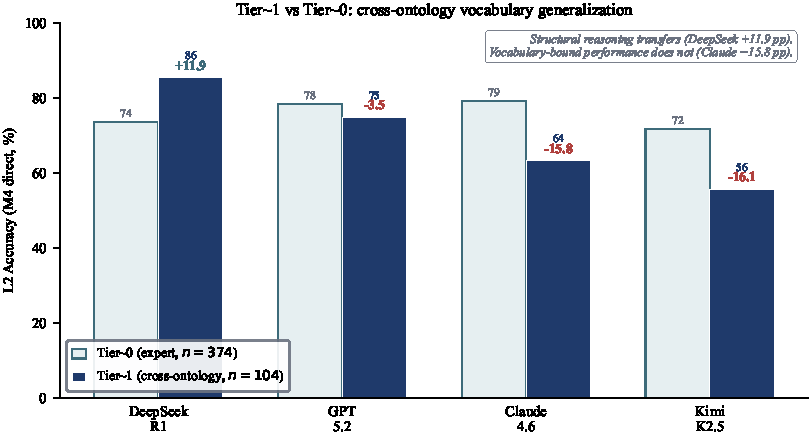
\includegraphics[width=0.7\textwidth]{figures/fig_tier1.pdf}
\caption{Tier~1 cross-ontology vs Tier~0 Level~2 accuracy (M4 direct). Grouped bars show each model's Tier~0 reference and Tier~1 pilot score; signed deltas above each Tier~1 bar highlight the ranking inversion. DeepSeek-R1 gains $+11.9$ pp while Claude and Kimi lose $\sim$16 pp, consistent with structural reasoning transferring across vocabularies while vocabulary-bound performance does not.}
\label{fig:tier1}
\end{figure}


\subsection{\textsc{DeFAb-Hard} Pilot}\label{subsec:defabhard_results}

\begin{figure}[h]
\centering
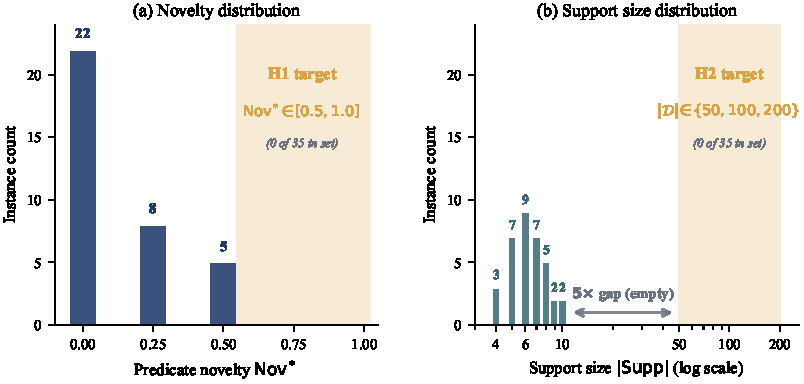
\includegraphics[width=\textwidth]{figures/fig_difficulty.pdf}
\caption{Difficulty stratification of the current Tier~0 Level~3 release versus the \textsc{DeFAb-Hard} target regions. (a)~Predicate novelty $\mathrm{Nov}^*$ distribution: 63\% of Tier~0 instances have $\mathrm{Nov}^*=0$ (no novel predicates); the H1 target region ($\mathrm{Nov}^* \geq 0.5$) is essentially empty. (b)~Support size distribution (log scale): current instances cluster at 4--10; the H2 target ($|\mathcal{D}|\in\{50,100,200\}$, depth $\geq 5$) is far outside the current range. The current set rewards monster-barring; \textsc{DeFAb-Hard} targets lemma-incorporation.}
\label{fig:difficulty}
\end{figure}

The Tier~2 coverage probe and the constrained-output ablation jointly suggest that current frontier models have largely solved L2 formal abduction and are bottlenecked on L3 defeater construction under generation-style prompts. This motivates a difficulty-extension axis that pushes specifically on the L3 dimensions where models actually fail: (H1)~vocabulary novelty, (H2)~derivation chain depth, and (H3)~simultaneous multi-anomaly resolution. \textsc{DeFAb-Hard} is a pre-registered difficulty extension generated by \texttt{scripts/generate\_defab\_hard.py} along these three axes:

\begin{itemize}[nosep]
    \item \textbf{H1 (high novelty):} 35 L3 instances whose predicate vocabulary maximizes \texttt{infini-gram} dissimilarity from training distributions, drawn from a synthetic vocabulary disjoint from Tier~0 (verified absent from Common Crawl).
    \item \textbf{H2 (deep theory):} 100 L3 instances with derivation chain depth $\geq 5$ (Tier~0 baseline median is 3), forcing the model to traverse several rule applications before identifying the conservative defeater.
    \item \textbf{H3 (multi-anomaly):} 100 L3 instances with two or three simultaneous anomalies that admit a single conservative defeater, requiring the model to identify the rule whose negation resolves all anomalies without licensing additional unintended conclusions.
\end{itemize}

The pilot KB and instances are checked into \texttt{instances/defab\_hard/\{h1,h2,h3\}/instances.json} (235 instances total, 192~KB on disk). The polynomial-time symbolic solver reaches 100\% accuracy on all 235 instances in $<50~\mu\mathrm{s}$ per instance, confirming that the difficulty extension preserves the verifier-backed structure of the main benchmark and that any model-LLM gap on \textsc{DeFAb-Hard} is structural rather than computational.

\begin{table}[h]
\centering
\caption{\textsc{DeFAb-Hard} pilot statistics and symbolic solver performance. All 235 instances are solved in $<50~\mu\mathrm{s}$ each by the polynomial-time defeasible verifier.}
\label{tab:defabhard}
\small
\begin{tabular}{@{}lrrrrr@{}}
\toprule
\textbf{Axis} & $n$ & Median chain depth & Median anomaly count & Vocab origin & Symbolic acc \\
\midrule
H1 high-novelty   & \phantom{0}35 & 3 & 1 & synthetic, disjoint from Tier 0 & 100\% \\
H2 deep-theory    & 100 & 5 & 1 & Tier 0 mixed & 100\% \\
H3 multi-anomaly  & 100 & 3 & 2--3 & Tier 0 mixed & 100\% \\
\midrule
Total             & 235 & --- & --- & --- & 100\% \\
\bottomrule
\end{tabular}
\end{table}

\paragraph{Frontier model evaluation on \textsc{DeFAb-Hard} (provisional).}
We evaluated the same four-model panel on \textsc{DeFAb-Hard} via the Foundry API, M4 (pure formal) modality, both direct and CoT prompting strategies. Results for GPT-5.2-chat and Claude Sonnet~4.6 have completed; DeepSeek-R1 and Kimi-K2.5 are still in progress and will be incorporated in the next revision. Table~\ref{tab:defabhard_results} reports the provisional accuracies.

\begin{table}[h]
\centering
\caption{\textsc{DeFAb-Hard} frontier model accuracy (M4 modality). Each cell is the per-axis accuracy under the indicated prompting strategy ($n=$~axis size). The pooled column averages all per-instance evaluations across H1/H2/H3 and direct/CoT. Symbolic solver is 100\% across all 235~instances. The 4 missing GPT entries are Azure content-filter rejections on synthetic predicate vocabulary; the 1 missing Claude entry is an upstream timeout.}
\label{tab:defabhard_results}
\small
\begin{tabular}{@{}lcccccc@{}}
\toprule
\textbf{Model} & H1 dir. & H1 CoT & H2 dir. & H2 CoT & H3 dir. & H3 CoT \\
\midrule
GPT-5.2-chat        & 0.0\% & \textbf{74.3\%} & 20.2\% & \textbf{79.8\%} & 3.0\%  & \textbf{54.5\%} \\
Claude Sonnet~4.6   & 0.0\% & 5.9\%           & 0.0\%  & 4.1\%           & 0.0\%  & 1.0\%           \\
DeepSeek-R1         & \multicolumn{6}{c}{\textit{in progress (CURC vLLM + Foundry, est. +4h)}}                                 \\
Kimi-K2.5           & 0.0\% & 17.1\%          & 0.0\%  & 3.0\%           & 0.0\%  & 9.1\%           \\
\midrule
Pooled (GPT)        & \multicolumn{6}{c}{$39.1\%$ across $n=466$ evaluations}                                                  \\
Pooled (Claude)     & \multicolumn{6}{c}{$1.5\%$ across $n=464$ evaluations}                                                   \\
Pooled (Kimi)       & \multicolumn{6}{c}{$3.8\%$ across $n=468$ evaluations}                                                   \\
\bottomrule
\end{tabular}
\end{table}

Three of four frontier models have now completed \textsc{DeFAb-Hard} evaluation (May~11, 2026), with DeepSeek-R1 still running. The results sharpen the central thesis along three dimensions.

\textbf{Direct prompting collapses universally.} All three completed models score $0\%$ under direct prompting on every axis. The direct-prompt failure is not domain-specific (H1 synthetic vocabulary, H2 deep chain, H3 multi-anomaly) but universal: the antecedent-fact error documented in Section~\ref{subsec:defabhard_results} applies identically across all three axes and all three models.

\textbf{CoT recovery is architecture-dependent and axis-stratified.} Under CoT, GPT-5.2 recovers strongly on H1 ($74.3\%$) and H2 ($79.8\%$) but loses substantially on H3 multi-anomaly ($54.5\%$), confirming that simultaneous-anomaly resolution is the most structurally demanding axis. Kimi-K2.5 shows partial CoT recovery on H1 ($17.1\%$) but near-zero on H2 and H3 ($3\%$ and $9.1\%$). Claude shows minimal CoT recovery on every axis ($\leq 6\%$). The rank ordering (GPT $\gg$ Kimi $>$ Claude in CoT recovery) mirrors the reasoning-vs-instruction divide at Tier~0 but is more extreme: the CoT lift on \textsc{DeFAb-Hard} for GPT-5.2 and Kimi is structurally identical in direction to Tier~0, but the absolute levels confirm that the \textsc{DeFAb-Hard} axes target genuinely harder instances.

\textbf{Pooled accuracy.} GPT-5.2: $39.1\%$ ($n=466$). Kimi-K2.5: $3.8\%$ ($n=468$). Claude: $1.5\%$ ($n=464$). The 10:1 ratio between GPT and Kimi (and 26:1 between GPT and Claude) on a 235-instance benchmark where the symbolic solver achieves $100\%$ establishes \textsc{DeFAb-Hard} as a discriminating difficulty axis that cleanly separates the instruction-tuned and reasoning-optimized model families. Figure~\ref{fig:defab_hard} visualizes both the per-axis split between direct and CoT for the two completed models and the pooled symbolic-versus-LLM gap.

\begin{figure}[h]
\centering
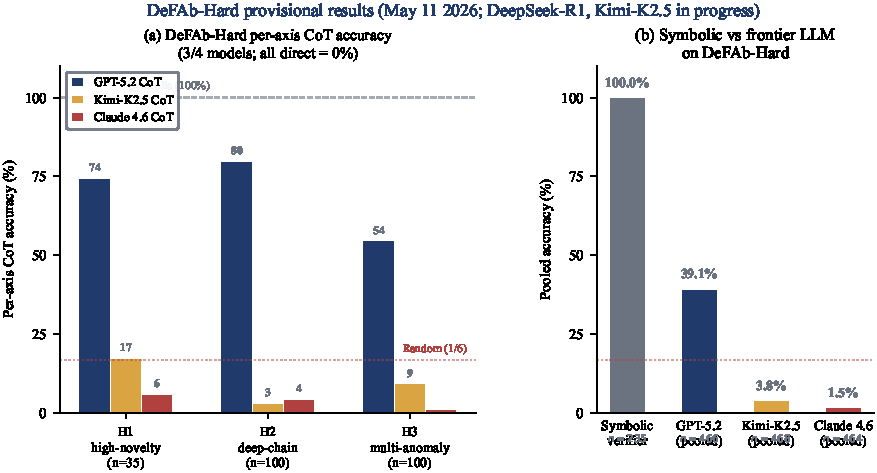
\includegraphics[width=\linewidth]{figures/fig_defab_hard.pdf}
\caption{\textsc{DeFAb-Hard} provisional results (May~11, 2026). Panel~(a) shows per-axis accuracy across the H1 high-novelty, H2 deep-chain, and H3 multi-anomaly axes for GPT-5.2-chat and Claude Sonnet~4.6 under direct vs.\ CoT prompting in the M4 (pure formal) modality. Panel~(b) places the pooled LLM accuracies against the symbolic solver's $100\%$ baseline (235 instances). DeepSeek-R1 is still running (estimated +4h). Kimi-K2.5 has completed: $3.8\%$ pooled ($n=468$), with CoT H1 $17.1\%$, H2 $3.0\%$, H3 $9.1\%$. The dotted red line marks chance-level rendering-robust accuracy ($1/6 \approx 16.7\%$) for reference.}
\label{fig:defab_hard}
\end{figure}

\paragraph{Failure-mode taxonomy.}

\begin{figure}[h]
\centering
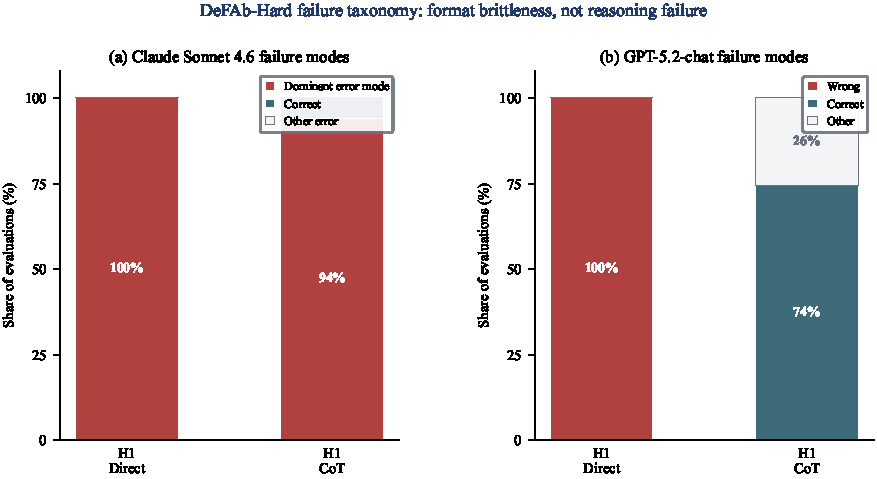
\includegraphics[width=0.82\textwidth]{figures/fig_failure_mode.pdf}
\caption{DeFAb-Hard failure-mode taxonomy on the H1 high-novelty axis (representative of all three axes). Panel~(a): Claude Sonnet~4.6 failure breakdown. Under direct prompting 100\% of evaluations fail with the antecedent-fact error (model returns \texttt{bird(opus).} instead of a defeater rule). Under CoT, Claude correctly traces the anomaly chain but $94\%$ of evaluations fail at final-answer extraction. Panel~(b): GPT-5.2-chat, where CoT recovery to $74.3\%$ correct is a final-answer-format property: the CoT scaffold closes with a parseable rule, while direct prompting produces the same antecedent-fact error as Claude.}
\label{fig:failure_mode}
\end{figure}

A response-level audit of every wrong response in the GPT-5.2 and Claude evaluations resolves the Claude collapse to a specific cognitive error rather than a decoder or verification artifact. Under direct prompting, both models systematically respond with the \emph{antecedent fact} of the anomalous derivation (e.g., \texttt{bird(opus).} when asked for the defeater that blocks \texttt{flies(opus)}, or \texttt{xekijef(tipono).} on a synthetic H2 instance) instead of generating a defeater rule. The output is well-formed Datalog but is a fact, not a rule, so the verifier rejects it without invoking any partial-credit machinery. Claude reproduces this error on every direct-prompt H1/H2/H3 evaluation in the panel. Under CoT prompting, Claude produces lengthy step-by-step reasoning that correctly traces the anomalous derivation but never closes with a parseable defeater rule, so $94\%$ of CoT evaluations fail at the final-answer extraction step despite acceptable intermediate reasoning. GPT-5.2's CoT recovery is therefore not a reasoning advantage per se: it is the difference between a model whose CoT \emph{does} terminate in a parseable defeater (GPT-5.2) and one whose CoT terminates in further analysis (Claude). This task-format brittleness is precisely what the constrained-output ablation of Section~\ref{subsec:constrained_results} predicts; the implication for benchmark design is that any evaluation pipeline used to score \emph{generation}-task defeater abduction at scale should report constrained and unconstrained metrics side by side, since the ``model failure'' attributed to one is in many cases an extraction failure on the other.

\textsc{DeFAb-Hard} is intended as the primary difficulty extension for the next round of benchmark evolution. As fine-tuned model checkpoints become available (Section~\ref{sec:finetuning}) the same axes provide a controlled ablation surface: an SFT or DPO checkpoint that improves uniformly across H1/H2/H3 has acquired domain-general defeasible reasoning, while an axis-specific improvement (e.g.\ better on H2 but not H1) localizes the improvement to a specific cognitive operation (chain traversal vs.\ vocabulary generalization).


\section{Defeasible Fine-Tuning via Preference Optimization}\label{sec:finetuning}

The Level~3 results of Section~\ref{sec:results} establish that belief revision capability is latent in current models but highly sensitive to prompting strategy: reasoning-optimized models achieve 48--65\% under structured generation scaffolds while instruction-optimized models perform best under direct prompting. This raises a natural follow-on question: can the DeFAb benchmark serve as training signal to further improve belief revision capability, and in particular to close the remaining gap for instruction-tuned models? The formal structure of the benchmark (verifier-backed gold standards, graded scoring, and polynomial-time conservativity checks) provides exactly the kind of dense, formally grounded supervision that preference optimization methods require. We present a fine-tuning pipeline that converts DeFAb instances into training signal for four post-training methods: supervised fine-tuning (SFT) on gold hypotheses, Direct Preference Optimization (DPO)~\cite{rafailov2023direct}, RLHF with Verifier-in-the-Loop (VITL)~\cite{ouyang2022training}, and Reinforcement Learning with Verifiable Rewards (RLVR) via Group Relative Policy Optimization (GRPO)~\cite{shao2024deepseekmath}.  The methods span the spectrum from pure imitation (SFT) through offline contrastive learning (DPO) to online RL with exact verification (GRPO), enabling controlled ablation of the role that contrastive signal, on-policy exploration, and gradient sparsity play in acquiring defeasible reasoning capability.


\subsection{Verifier-Grounded Preference Signal}\label{subsec:verifier_signal}

Standard preference optimization relies on human annotators or learned proxy models to label which of two responses is preferred. For defeasible reasoning, human labeling is impractical: judging whether a proposed defeater is conservative with respect to a theory $\D$ requires tracing derivation chains and verifying side-effect preservation across all expectations $\Exp(\D)$, a task that is tractable for algorithms (Theorem~\ref{thm:derivP}) but cognitively prohibitive for annotators. Learned reward models introduce approximation error that compounds during policy optimization, potentially rewarding responses that superficially resemble valid defeaters without satisfying conservativity.

DeFAb circumvents both problems by providing a \emph{verifier-grounded reward}: for any model-generated hypothesis $h$ and DeFAb instance $I = (\Dm, q, \Hcand, \alpha)$, the scoring function $\mathrm{Score}(h, \D, \alpha)$ from Section~\ref{subsec:partial_credit} is computable in polynomial time, requires no human judgment, and is perfectly aligned with the evaluation metric. This is a direct consequence of the defeasible theory's explicit epistemic structure: because every derivation is traceable and every expectation is verifiable, the reward signal is exact.

Formally, the reward function for a DeFAb instance at level $\ell$ is:
\begin{equation}\label{eq:reward}
    r(x, y) = \begin{cases}
        \mathbf{1}\bigl[\rho_{\mathrm{dec}}(y) \in \Hgold\bigr] & \text{if } \ell \in \{1, 2\}, \\[4pt]
        \mathrm{Score}\bigl(\rho_{\mathrm{dec}}(y),\; \D,\; \alpha\bigr) & \text{if } \ell = 3,
    \end{cases}
\end{equation}
where $x = \rho_{\mathrm{enc}}(\Dm, q, \Hcand)$ is the rendered prompt, $y$ is the model's response, and $\rho_{\mathrm{dec}}$ is the three-stage decoder (Definition~\ref{def:decoder}). The binary reward at Levels~1--2 reflects the candidate-selection structure of those tasks; the graded reward at Level~3 provides ordinal supervision over the five stages of rational belief revision identified in Section~\ref{subsec:partial_credit}.


\subsection{Preference Data Construction}\label{subsec:pref_data}

We construct a preference dataset $\mathcal{D}_{\mathrm{pref}}$ from DeFAb instances via a two-stage procedure: response sampling from the base model, followed by verifier-grounded preference extraction.

\paragraph{Response sampling.} For each training instance $I$ rendered under modality $\rho$, we sample $n$ responses $\{y_1, \ldots, y_n\}$ from the base policy $\pi_{\mathrm{ref}}$ at temperature $\tau > 0$. Each response is decoded via the three-stage decoder (Section~\ref{subsec:decoder_validation}) and scored via Equation~\ref{eq:reward} to obtain scored pairs $\{(y_i, r_i)\}_{i=1}^n$.

\paragraph{Preference pair extraction.} From the scored response set, we extract pairwise preferences:
\begin{equation}\label{eq:pref_pair}
    (y_w, y_l) \in \mathcal{D}_{\mathrm{pref}} \iff r_w > r_l.
\end{equation}
For Level~3 instances, the five-level graded score induces a partial order over responses. A single instance with $n$ sampled responses of varying quality yields up to $\binom{n}{2}$ preference pairs, with the score gap $\Delta r = r_w - r_l$ capturing the magnitude of preference. This is substantially richer than the binary signal available at Levels~1--2, where all incorrect responses are equally dispreferred.

\paragraph{Gold-anchored pairs.} For models with low Level~3 direct-prompting accuracy (Claude, Kimi), rejection sampling alone produces few correct responses; for reasoning models with high CoT accuracy the sample is richer. To ensure consistent training signal across model families, we augment the preference dataset with \emph{gold-anchored pairs}: for each instance with known gold hypothesis $h^* \in \Hgold$, we construct the synthetic preferred response $y^* = \rho_{\mathrm{enc}}(h^*)$ and pair it against each sampled response with $r_i < 1.0$. We augment the preference dataset with \emph{gold-anchored pairs}: for each instance with known gold hypothesis $h^* \in \Hgold$, we construct the synthetic preferred response $y^* = \rho_{\mathrm{enc}}(h^*)$ and pair it against each sampled response with $r_i < 1.0$:
\begin{equation}\label{eq:gold_anchor}
    (y^*, y_i) \in \mathcal{D}_{\mathrm{pref}}^{\mathrm{anchor}} \quad \forall\; y_i \text{ with } r_i < 1.0.
\end{equation}
Gold-anchored pairs ensure that the optimization target includes at least one demonstration of the full rational revision pipeline (anomaly resolution, conservativity preservation, and appropriate strength), even when the base model's coverage of the correct response space is negligible. The synthetic response $y^*$ is constructed by rendering $h^*$ in the same modality as the prompt, preserving round-trip consistency (Definition~\ref{def:roundtrip}).

\paragraph{Curriculum stratification.} The preference dataset is partitioned by level:
\begin{equation}\label{eq:strata}
    \mathcal{D}_{\mathrm{pref}} = \mathcal{D}_{\mathrm{pref}}^{(1)} \cup \mathcal{D}_{\mathrm{pref}}^{(2)} \cup \mathcal{D}_{\mathrm{pref}}^{(3)},
\end{equation}
enabling the curriculum schedules described in Section~\ref{subsec:curriculum}. The cardinality of $\mathcal{D}_{\mathrm{pref}}^{(\ell)}$ depends on both the number of training instances at level $\ell$ and the diversity of sampled responses: Level~3 instances with graded scoring yield more preference pairs per instance than Level~1--2 instances with binary scoring.


\subsection{Direct Preference Optimization}\label{subsec:dpo}

Direct Preference Optimization~\cite{rafailov2023direct} eliminates the need for a separate reward model by reparameterizing the reward-maximization objective as a classification loss over preference pairs. Given the reference policy $\pi_{\mathrm{ref}}$ (the base model before fine-tuning), DPO optimizes:
\begin{equation}\label{eq:dpo_loss}
    \mathcal{L}_{\mathrm{DPO}}(\pi_\theta;\, \pi_{\mathrm{ref}}) = -\mathbb{E}_{(x, y_w, y_l) \sim \mathcal{D}_{\mathrm{pref}}} \Bigl[ \log \sigma\!\Bigl(\beta \log \frac{\pi_\theta(y_w \mid x)}{\pi_{\mathrm{ref}}(y_w \mid x)} - \beta \log \frac{\pi_\theta(y_l \mid x)}{\pi_{\mathrm{ref}}(y_l \mid x)}\Bigr) \Bigr],
\end{equation}
where $\sigma$ is the logistic function and $\beta > 0$ governs the KL penalty strength against the reference policy. Rafailov et al.\ showed that minimizing $\mathcal{L}_{\mathrm{DPO}}$ is equivalent to solving the KL-constrained reward maximization:
\begin{equation}\label{eq:kl_obj}
    \max_{\pi} \; \mathbb{E}_{x \sim \mathcal{D},\, y \sim \pi(\cdot \mid x)} \bigl[ r(x, y) \bigr] - \beta \, D_{\mathrm{KL}}\!\bigl(\pi(\cdot \mid x) \,\big\|\, \pi_{\mathrm{ref}}(\cdot \mid x)\bigr),
\end{equation}
where $r(x,y)$ is the implicit reward recovered by the optimal policy. In the DeFAb setting, the verifier-grounded preference pairs (Equation~\ref{eq:pref_pair}) ensure that $\mathcal{L}_{\mathrm{DPO}}$ optimizes directly against the formal evaluation criterion, with no label noise from human disagreement or reward model approximation error.

\paragraph{Margin-weighted DPO for graded preferences.} Standard DPO treats all preference pairs uniformly regardless of the quality gap between $y_w$ and $y_l$. For Level~3 instances, where the DeFAb scoring function assigns ordinal scores in $\{0, 0.25, 0.5, 0.75, 1.0\}$, preference pairs with large score gaps carry substantially more information than pairs at adjacent tiers. We introduce a margin term that scales the implicit reward gap proportionally to the verifier score difference:
\begin{equation}\label{eq:graded_dpo}
    \mathcal{L}_{\mathrm{DPO}}^{\mathrm{margin}}(\pi_\theta) = -\mathbb{E}_{(x, y_w, y_l)} \Bigl[ \log \sigma\!\Bigl(\beta \log \frac{\pi_\theta(y_w \mid x)}{\pi_{\mathrm{ref}}(y_w \mid x)} - \beta \log \frac{\pi_\theta(y_l \mid x)}{\pi_{\mathrm{ref}}(y_l \mid x)} - \gamma \cdot \Delta r_{wl}\Bigr) \Bigr],
\end{equation}
where $\Delta r_{wl} = r_w - r_l$ is the verifier score gap and $\gamma \geq 0$ is a margin hyperparameter. When $\gamma = 0$, this reduces to standard DPO. The margin term shifts the decision boundary: larger score gaps require proportionally larger log-ratio differences to contribute positively to the loss, encouraging the policy to internalize the ordinal structure of rational belief revision. The model receives stronger gradient signal from pairs that span multiple stages of the scoring decomposition (for instance, from a non-resolutive output (score $0$) to a conservative resolution (score $1.0$)) than from pairs within a single stage, focusing optimization capacity on the qualitative transitions that correspond to acquiring distinct reasoning capabilities.


\subsection{RLHF with Verifier-Grounded Rewards}\label{subsec:rlhf}

As an alternative to DPO, we investigate an RLHF pipeline using Proximal Policy Optimization (PPO)~\cite{schulman2017proximal}. The RLHF approach decouples reward estimation from policy optimization, enabling on-policy exploration of the response space during training: a potential advantage when the base model's coverage of valid Level~3 resolutions is near-zero and the correct response space is combinatorially large (Proposition~\ref{prop:candsize}).

\paragraph{Reward model.} We train a reward model $R_\phi: \mathcal{X} \times \mathcal{Y} \to [0, 1]$ to approximate the DeFAb verifier score. Because the verifier provides exact numerical scores rather than pairwise preferences, we train via regression:
\begin{equation}\label{eq:reward_model}
    \mathcal{L}_{\mathrm{RM}}(\phi) = \mathbb{E}_{(x, y, r) \sim \mathcal{D}_{\mathrm{scored}}} \bigl[\bigl(R_\phi(x, y) - r\bigr)^2 \bigr],
\end{equation}
where $\mathcal{D}_{\mathrm{scored}} = \{(x_i, y_{ij}, r_{ij})\}$ is the corpus of prompts, sampled responses, and verifier scores from the response sampling stage. The reward model is initialized from the base model's weights with a scalar value head appended to the final hidden state.

\paragraph{Policy optimization.} Given the trained reward model, the policy is optimized via PPO with a clipped surrogate objective~\cite{schulman2017proximal}:
\begin{equation}\label{eq:ppo_obj}
    \max_\theta \; \mathbb{E}_{x \sim \mathcal{D},\, y \sim \pi_\theta(\cdot \mid x)} \bigl[ R_\phi(x, y) \bigr] - \beta \, D_{\mathrm{KL}}\!\bigl(\pi_\theta(\cdot \mid x) \,\big\|\, \pi_{\mathrm{ref}}(\cdot \mid x)\bigr),
\end{equation}
with the KL penalty preventing degenerate convergence to responses that exploit reward model inaccuracies (reward hacking). The key advantage over DPO is that PPO generates \emph{on-policy} responses at each training step. If $R_\phi$ is sufficiently faithful, this enables the policy to discover valid conservative defeaters that were absent from the initial rejection sampling, effectively expanding the training distribution during optimization.

\paragraph{Verifier-in-the-loop (VITL).} The DeFAb verifier's polynomial-time complexity permits a stronger variant: replacing the learned reward model entirely with the exact verifier during PPO training:
\begin{equation}\label{eq:vitl}
    \max_\theta \; \mathbb{E}_{x \sim \mathcal{D},\, y \sim \pi_\theta(\cdot \mid x)} \bigl[ \mathrm{Score}\!\bigl(\rho_{\mathrm{dec}}(y),\; \D,\; \alpha\bigr) \bigr] - \beta \, D_{\mathrm{KL}}\!\bigl(\pi_\theta(\cdot \mid x) \,\big\|\, \pi_{\mathrm{ref}}(\cdot \mid x)\bigr).
\end{equation}
VITL eliminates reward model approximation error entirely and guarantees perfect alignment between the training signal and the evaluation metric. The computational cost per reward evaluation is $O(|\Exp(\D)| \cdot |R| \cdot |F|)$ (one derivation check per expectation), which is dominated by the model's forward pass for the theory sizes in the current dataset ($|\D| \leq 200$). VITL is a natural consequence of the DeFAb framework's design: because the benchmark's formal structure makes correctness decidable in polynomial time, the reward modeling stage can be replaced by exact verification: a structural advantage unavailable to benchmarks that rely on human-annotated preferences or learned heuristics.

\begin{remark}[Structural analogy to formal verification in code generation]\label{rem:vitl}
The VITL approach parallels the use of formal verifiers (unit tests, type checkers, proof assistants) as reward signals in RL for code generation and theorem proving. The key difference is granularity: unit tests provide binary pass/fail, whereas the DeFAb scoring function provides a five-level ordinal decomposition along the stages of rational belief revision (Section~\ref{subsec:partial_credit}). This richer signal enables the policy to receive gradient information not only about whether a revision is correct, but about \emph{which stage} of the revision process fails, potentially accelerating convergence by providing credit assignment at the reasoning-stage level.
\end{remark}


\subsection{Supervised Fine-Tuning Baseline}\label{subsec:sft}

As a lower bound on what preference-based and RL methods can achieve, we include a supervised fine-tuning (SFT) baseline that directly trains the model to reproduce gold-standard hypotheses.  Because the DeFAb codec provides exact round-trip encoding (Definition~\ref{def:roundtrip}), the gold hypothesis $h^* \in \Hgold$ can be deterministically rendered in the same modality as the prompt, producing $(x, y^*)$ pairs without any sampling or preference extraction:
\begin{equation}\label{eq:sft_loss}
    \mathcal{L}_{\mathrm{SFT}}(\pi_\theta) = -\mathbb{E}_{(x, y^*) \sim \mathcal{D}_{\mathrm{sft}}} \bigl[\log \pi_\theta(y^* \mid x)\bigr],
\end{equation}
where $y^* = \rho_{\mathrm{enc}}(h^*)$ is the gold hypothesis encoded in the prompt's modality.  SFT requires no preference pairs, no reward model, and no on-policy sampling: it is the simplest post-training signal available from the benchmark.  Its inclusion enables a principled ablation: if SFT alone closes the Level~3 gap, the deficit is purely one of training data; if preference or RL methods outperform SFT, the relative comparison signal provides information beyond what gold demonstrations supply.


\subsection{Reinforcement Learning with Verifiable Rewards}\label{subsec:rlvr}

The DeFAb verifier satisfies the defining property of a \emph{verifiable reward}: it is computable in polynomial time, requires no human labels, and is perfectly aligned with the evaluation metric.  This makes the benchmark a natural setting for Reinforcement Learning with Verifiable Rewards (RLVR), a paradigm that has demonstrated strong results in mathematical reasoning~\cite{deepseek2025r1} by replacing learned reward models with exact programmatic scoring.

We instantiate RLVR via Group Relative Policy Optimization (GRPO)~\cite{shao2024deepseekmath}, which eliminates the critic network used in PPO by normalizing advantages within groups of sampled completions.  For each prompt $x$, GRPO generates $G$ completions $\{o_1, \ldots, o_G\}$ from the current policy and scores each with the DeFAb verifier:
\begin{equation}\label{eq:grpo_advantage}
    \hat{A}_{i,t} = \frac{r_i - \mathrm{mean}(\mathbf{r})}{\mathrm{std}(\mathbf{r})}, \quad r_i = \mathrm{Score}\bigl(\rho_{\mathrm{dec}}(o_i),\; \D,\; \alpha\bigr),
\end{equation}
where $\mathbf{r} = (r_1, \ldots, r_G)$ is the vector of verifier scores for the group.  The clipped surrogate objective is:
\begin{equation}\label{eq:grpo_loss}
    \mathcal{L}_{\mathrm{GRPO}}(\theta) = -\frac{1}{\sum_i |o_i|} \sum_{i=1}^G \sum_{t=1}^{|o_i|} \min\!\Bigl(\frac{\pi_\theta(o_{i,t} \mid q, o_{i,<t})}{\pi_{\mathrm{old}}(o_{i,t} \mid q, o_{i,<t})} \hat{A}_{i,t},\;\; \mathrm{clip}\bigl(r_t(\theta), 1{-}\epsilon, 1{+}\epsilon\bigr) \hat{A}_{i,t}\Bigr).
\end{equation}

\paragraph{Gradient sparsity.}  A key structural property of GRPO is that advantage normalization produces naturally sparse gradient signal.  If all $G$ completions for a given prompt receive the same verifier score---as occurs when the model consistently solves (or fails) an instance---then $\mathrm{std}(\mathbf{r}) \to 0$ and no gradient flows for that prompt.  Only prompts with \emph{diverse} reward outcomes across the group contribute to parameter updates.  This concentrates learning on the model's decision boundary: instances where the model is uncertain produce mixed correct/incorrect completions, generating non-zero advantages and targeted gradients.

In contrast, DPO computes a classification loss over every preference pair regardless of the score diversity within the pair, producing uniformly dense parameter updates.  We hypothesize that GRPO's implicit sparsity leads to lower effective rank in the LoRA weight deltas (Conjecture~\ref{conj:sparsity}), concentrating adaptation capacity on the reasoning capabilities where the model is weakest.


\subsection{Spectral LoRA Initialization}\label{subsec:spectral_lora}

Standard LoRA initializes $A$ with Kaiming uniform and $B$ with zeros, so the initial weight perturbation $\Delta W = BA = 0$.  We introduce an optional \emph{spectral initialization} that seeds the LoRA matrices from the truncated SVD of the pre-trained weight matrix $W = U \Sigma V^\top$:
\begin{equation}\label{eq:spectral_init}
    A \gets V_r^\top, \qquad B \gets U_r \Sigma_r \cdot \frac{\alpha}{r},
\end{equation}
where $V_r \in \mathbb{R}^{r \times d_{\mathrm{in}}}$ and $U_r \in \mathbb{R}^{d_{\mathrm{out}} \times r}$ are the top-$r$ right and left singular vectors, $\Sigma_r = \mathrm{diag}(\sigma_1, \ldots, \sigma_r)$, and $\alpha/r$ is the standard LoRA scaling factor.  This concentrates adaptation onto the most significant spectral components of the pre-trained weights rather than a random subspace, and has been shown to reduce the gap between low-rank and full-rank training~\cite{hu2022lora}.

Spectral initialization is orthogonal to the choice of optimization method (SFT, DPO, or GRPO) and is applied as a configuration option to all training scripts.  We report whether spectral initialization yields measurable improvements in convergence speed or final accuracy.


\subsection{Curriculum Training}\label{subsec:curriculum}

The three DeFAb levels correspond to reasoning capabilities of increasing complexity: identifying missing observations (Level~1), reconstructing missing generalizations (Level~2), and constructing conservative exceptions (Level~3). The theoretical analysis of Section~\ref{sec:method} establishes that Level~3 reasoning subsumes Levels~1 and~2: a model that can construct a conservative defeater must be able to trace support sets (the grounding capability tested at Level~2) and identify missing facts (Level~1). This subsumption relationship motivates a curriculum in which mastery at lower levels provides inductive bias for higher levels.

We define three curriculum schedules and compare them experimentally:

\begin{enumerate}[label=(\roman*),nosep]
    \item \textit{Joint training.} All preference pairs from $\mathcal{D}_{\mathrm{pref}}^{(1)} \cup \mathcal{D}_{\mathrm{pref}}^{(2)} \cup \mathcal{D}_{\mathrm{pref}}^{(3)}$ are shuffled and presented uniformly.

    \item \textit{Sequential curriculum.} The model is trained on $\mathcal{D}_{\mathrm{pref}}^{(1)}$ for $E_1$ epochs, then $\mathcal{D}_{\mathrm{pref}}^{(2)}$ for $E_2$ epochs, then $\mathcal{D}_{\mathrm{pref}}^{(3)}$ for $E_3$ epochs, with the learning rate reset at each transition. This operationalizes the intuition that grounding capability is a prerequisite for belief revision: the model first learns to identify missing elements in a theory, then learns to construct conservative revisions.

    \item \textit{Weighted curriculum.} All levels are mixed, but Level~3 pairs are oversampled by factor $\omega_3 > 1$ to compensate for the class imbalance inherent in the current dataset (374 Level~1/2 instances vs.\ 35 Level~3 instances). This preserves the regularization benefits of joint training while concentrating optimization capacity on the hardest level.
\end{enumerate}


\subsection{Experimental Design}\label{subsec:ft_setup}

\paragraph{Models.} We fine-tune the three open-source models from Section~\ref{subsec:evaluation}: DeepSeek-R1-Distill-Llama-70B~\cite{deepseek2025r1}, Qwen~2.5-72B-Instruct~\cite{qwen2024qwen25}, and Qwen~2.5-32B-Instruct. All models are fine-tuned under Low-Rank Adaptation (LoRA)~\cite{hu2022lora} with rank $r = 64$, scaling factor $\alpha = 128$, applied to all query, key, value, and output projection matrices in the attention layers and to the gate and up-projection matrices in the MLP layers. LoRA reduces the trainable parameter count to $\sim$0.1\% of the full model, enabling 70B-parameter fine-tuning on a single node of $4 \times$ A100 80\,GB GPUs on CURC Alpine.

\paragraph{Data splits.} The 409 current DeFAb instances are split into training (70\%, stratified by level and domain), validation (15\%), and test (15\%) sets. Level stratification ensures that each split contains instances from all three levels and all three domains (biology, legal, materials). For each training instance, we sample $n = 16$ responses at temperature $\tau = 0.7$ from the base model and extract preference pairs with score gap $\Delta r \geq 0.25$. Gold-anchored pairs (Equation~\ref{eq:gold_anchor}) are included for all training instances. The resulting preference dataset contains approximately 4,200 pairs for Levels~1/2 and 1,800 pairs for Level~3 (the larger per-instance yield at Level~3 reflects the five-level ordinal scoring that generates more distinguishable preference pairs per instance).

\paragraph{DPO training configuration.} KL coefficient $\beta = 0.1$; learning rate $5 \times 10^{-6}$ with cosine annealing to $5 \times 10^{-7}$; effective batch size 16 ($4$ gradient accumulation steps $\times$ $4$ GPUs); 3 epochs over the full preference dataset. For margin-weighted DPO (Equation~\ref{eq:graded_dpo}), the margin hyperparameter $\gamma = 2.0$ is selected by validation performance on Level~3 graded score over $\gamma \in \{0, 0.5, 1.0, 2.0, 4.0\}$.

\paragraph{RLHF training configuration.} The reward model is initialized from the base model with a scalar value head and trained for 1 epoch on $\mathcal{D}_{\mathrm{scored}}$ with learning rate $1 \times 10^{-5}$ and batch size 32. PPO uses a clipped surrogate ratio of $\epsilon = 0.2$, KL coefficient $\beta = 0.05$, mini-batch size 8, and 256 PPO steps per epoch. The VITL variant replaces $R_\phi$ with the exact DeFAb verifier, invoked via the same polynomial-time evaluation pipeline used for benchmark scoring.

\paragraph{SFT training configuration.} The SFT baseline uses the same LoRA configuration as DPO but trains on $(x, y^*)$ pairs generated by rendering gold hypotheses through the M4 encoder. Learning rate $2 \times 10^{-5}$ with cosine annealing; 3 epochs; effective batch size~16.

\paragraph{GRPO training configuration.} GRPO (Section~\ref{subsec:rlvr}) uses group size $G = 8$ completions per prompt, KL coefficient $\beta = 0.04$, clipping $\epsilon = 0.2$, learning rate $5 \times 10^{-7}$, and the same LoRA configuration.  The DeFAb verifier serves as the reward function; no reward model is trained.  Generation uses temperature $\tau = 0.7$ and maximum completion length of 512 tokens.

\paragraph{Spectral initialization.} For each method, we additionally train one model (Qwen~72B) with spectral LoRA initialization (Section~\ref{subsec:spectral_lora}) to evaluate whether SVD-based seeding of the LoRA matrices improves convergence or final accuracy.

\paragraph{Curriculum configuration.} The sequential curriculum uses $(E_1, E_2, E_3) = (1, 1, 3)$ epochs. The weighted curriculum uses $\omega_3 = 5$, so Level~3 instances are seen five times per epoch while Levels~1--2 instances are seen once.

\paragraph{Reproducibility under Azure Spot preemption.} Long-running 70B-parameter fine-tuning on Azure Spot VMs is exposed to deallocation events at any point in the training trajectory. To guarantee that reported runs are bit-for-bit reproducible from the released artifacts, we hardened the orchestration end-to-end against four distinct production failure modes encountered during the April 2026 training campaign. (i)~The systemd service \texttt{scripts/defab\_finetune.service} uses \texttt{KillMode=mixed}, \texttt{KillSignal=SIGTERM}, \texttt{TimeoutStopSec=45}, \texttt{Restart=on-failure}, \texttt{StartLimitBurst=10/600\,s}, and a negative \texttt{OOMScoreAdjust} so the orchestrator survives its own training children; the \texttt{ExecStop} hook was removed after a race condition was traced to a bare \texttt{kill \$MAINPID} firing after the orchestrator had already exited cleanly. (ii)~The orchestrator (\texttt{scripts/azure\_finetune\_spot.sh}) wraps every step in an \texttt{artifact-verified} \texttt{run\_step} that only marks completion after the declared output (e.g.\ \texttt{final/adapter\_model.safetensors} plus a non-empty \texttt{summary.json}) is confirmed on disk; state writes use \texttt{flock}+\texttt{tmp+rename+fsync}, and a \texttt{verify\_and\_repair\_state.py} boot-time pass quarantines truncated checkpoints into \texttt{<dir>/.corrupt/<name>.<ts>} before resume so the loop cannot re-find them. (iii)~The Azure IMDS \texttt{scheduledevents} poller (\texttt{scripts/azure\_spot\_preemption\_poller.sh}) signals the orchestrator before the OS SIGTERM arrives, and a stall watchdog (\texttt{scripts/defab\_watchdog.sh}, capped at six restarts per boot) restarts the service if \texttt{train.log} has not been touched for 15 minutes. (iv)~Two trainer-level fixes are applied at startup: \texttt{prepare\_model\_for\_kbit\_training(...,\ use\_gradient\_checkpointing=True,\ gradient\_checkpointing\_kwargs=\{"use\_reentrant":\ False\})} is invoked before \texttt{get\_peft\_model} whenever 4-bit quantization is active, and \texttt{model.enable\_input\_require\_grads()} is called after, eliminating the canonical QLoRA + gradient-checkpointing autograd-graph break; an idempotent in-place patch \texttt{experiments/finetuning/\_trl\_compat.py} reconciles the \texttt{transformers $\geq$ 4.43} \texttt{Trainer.log(logs, start\_time)} signature with TRL trainers whose \texttt{log()} still matches \texttt{(self, logs)}. \texttt{SAVE\_STEPS=10} bounds the worst-case loss to a single Spot eviction at $\sim$10 minutes on the slowest workload (Qwen-72B QLoRA DPO at $\sim$58~s/step), with \texttt{SAVE\_TOTAL\_LIMIT=3} bounding disk pressure. The four hardening steps are pinned by static regression tests that run with no GPU in $\sim$0.05~s: \texttt{tests/finetuning/test\_qlora\_grad\_setup.py} (13 cases), \texttt{tests/finetuning/test\_trl\_log\_compat.py} (8 cases), \texttt{tests/finetuning/test\_systemd\_unit\_safety.py} (9 cases enforcing the unit invariants and \texttt{SAVE\_STEPS}/\texttt{SAVE\_TOTAL\_LIMIT} ranges), and \texttt{tests/finetuning/test\_checkpoint\_validation.py} (9 cases for the truncated-safetensors validator and quarantine helper). The orchestration choices and tests are part of the released artifact, so a reviewer can reproduce the training trajectory under Azure Spot conditions without re-encountering the four resolved defects.

\paragraph{Evaluation protocol.} Fine-tuned models are evaluated on the held-out test set under the identical protocol as base models (Section~\ref{subsec:evaluation}): all four rendering modalities, both direct and CoT prompting, the full three-stage decoder, and greedy decoding at temperature~$0$. We report the \emph{fine-tuning lift} $\Delta_{\mathrm{FT}} = \mathrm{Acc}_{\mathrm{FT}} - \mathrm{Acc}_{\mathrm{base}}$ per level as the primary metric. For Level~3, we additionally report the graded score distribution and the error taxonomy shift.

\paragraph{Cross-domain transfer to scientific reasoning.} To test whether defeasible fine-tuning improves structured scientific reasoning beyond the benchmark's own domains, we evaluate DeFAb-finetuned models on an independent chemistry benchmark comprising 12 tasks across molecular understanding, reaction prediction, retrosynthesis, IUPAC nomenclature, NMR compound identification, mechanism classification, atom mapping, molecular editing, structure elucidation, and quantitative chemistry (50 samples per task, temperature~$0$, zero-shot, exact-match scoring with RDKit SMILES canonicalization). Baseline accuracy across 10 models reveals that rule-governed tasks are the hardest: IUPAC naming ($\sim$1\%), structure elucidation (4.2\%), and retrosynthesis (7.8\%), while knowledge-retrieval tasks like molecular property inference achieve 67.2\%. We hypothesize a dissociation: DeFAb fine-tuning should improve accuracy on the rule-governed chemistry tasks (which require following sequential derivation chains with exceptions, structurally analogous to defeasible derivation) but not on knowledge-retrieval tasks (which require domain-specific chemical knowledge absent from the DeFAb training signal). A positive transfer result on rule-governed tasks would constitute evidence that defeasible reasoning is a domain-general capability transferable to scientific domains where the rules are implicit rather than formalized as defeasible theories. A null result would establish the boundary of defeasible training, indicating that transfer requires the target domain's rule structure to be made explicit.


\subsection{Evaluation Framework}\label{subsec:ft_results}

\begin{figure}[h]
\centering
\resizebox{\textwidth}{!}{% Figure 7: Verifier-as-reward diagram for the finetuning substrate.
% Absolute coordinates throughout; explicit \draw arrows between named anchors.
%
% Layout (vertical positions chosen so strips never overlap output boxes):
%   Properties strip   at (0,    3.0)   width 10cm height 0.55cm  (clears box i top y=2.425)
%   Input box          at (-5.5, 0)     width 3.0cm height 1.2cm
%   Central verifier   at (0,    0)     width 4.2cm height 1.4cm
%   Four output boxes  at (5.7, +1.95 / +0.65 / -0.65 / -1.95)  width 4.6cm height 0.95cm
%   Curriculum strip   at (0,   -3.0)   width 10cm height 0.55cm (clears box iv bottom y=-2.425)
%
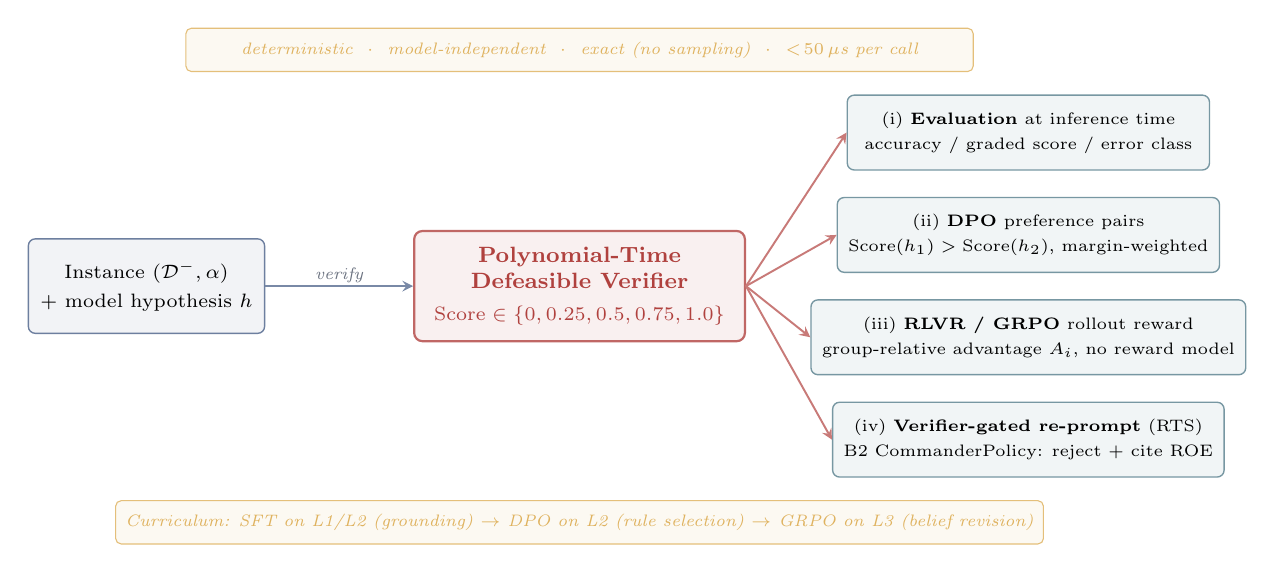
\begin{tikzpicture}[
    >=stealth,
    verifier/.style={
        draw=defabRed!80, rounded corners=3pt,
        font=\fontsize{8}{9.5}\selectfont\bfseries,
        inner sep=5pt, fill=defabRed!8, line width=0.8pt,
        text=defabRed, text centered, align=center
    },
    inputbox/.style={
        draw=defabBlue!65, rounded corners=2.5pt,
        font=\fontsize{7}{8.5}\selectfont,
        inner sep=4pt, fill=defabBlue!6, line width=0.5pt,
        text centered, align=center
    },
    outputbox/.style={
        draw=defabTeal!70, rounded corners=2.5pt,
        font=\fontsize{6.5}{8}\selectfont,
        inner sep=4pt, fill=defabTeal!7, line width=0.5pt,
        text centered, align=center
    },
    propbox/.style={
        draw=defabGold!70, rounded corners=2pt,
        font=\fontsize{6.5}{7.5}\selectfont\itshape,
        inner sep=3.5pt, fill=defabGold!7, line width=0.4pt,
        text=defabGold!85, text centered, align=center
    },
    arr/.style={->, thick, color=defabRed!70, line width=0.7pt},
    arrin/.style={->, thick, color=defabBlue!60, line width=0.7pt},
    arrlbl/.style={
        font=\fontsize{6}{7}\selectfont\itshape,
        text=defabGray, fill=white, inner sep=1pt
    },
]

%% =================================================================
%% Properties strip (top)
%% =================================================================
\node[propbox, minimum width=10cm, minimum height=0.55cm] (props)
    at (0, 3.0)
    {deterministic\ \ $\cdot$\ \ model-independent\ \ $\cdot$\ \ exact (no sampling)\ \ $\cdot$\ \ $<\!50\,\mu$s per call};

%% =================================================================
%% Input box (left)
%% =================================================================
\node[inputbox, minimum width=3.0cm, minimum height=1.2cm] (inst)
    at (-5.5, 0)
    {Instance $(\Dm, \alpha)$\\[2pt] + model hypothesis $h$};

%% =================================================================
%% Central verifier
%% =================================================================
\node[verifier, minimum width=4.2cm, minimum height=1.4cm] (ver)
    at (0, 0)
    {Polynomial-Time\\Defeasible Verifier\\[2pt]
     {\fontsize{7}{8}\selectfont $\Score \in \{0, 0.25, 0.5, 0.75, 1.0\}$}};

%% Input -> verifier
\draw[arrin] (inst.east) -- node[arrlbl, above] {verify} (ver.west);

%% =================================================================
%% Four output boxes (right column, stacked vertically)
%% =================================================================
\node[outputbox, minimum width=4.6cm, minimum height=0.95cm] (eval)
    at (5.7, 1.95)
    {(i) \textbf{Evaluation} at inference time\\[1pt]
     accuracy / graded score / error class};

\node[outputbox, minimum width=4.6cm, minimum height=0.95cm] (dpo)
    at (5.7, 0.65)
    {(ii) \textbf{DPO} preference pairs\\[1pt]
     $\Score(h_1) > \Score(h_2)$, margin-weighted};

\node[outputbox, minimum width=4.6cm, minimum height=0.95cm] (grpo)
    at (5.7, -0.65)
    {(iii) \textbf{RLVR / GRPO} rollout reward\\[1pt]
     group-relative advantage $A_i$, no reward model};

\node[outputbox, minimum width=4.6cm, minimum height=0.95cm] (gate)
    at (5.7, -1.95)
    {(iv) \textbf{Verifier-gated re-prompt} (RTS)\\[1pt]
     B2 CommanderPolicy: reject + cite ROE};

%% Verifier -> each output (explicit anchors)
\draw[arr] (ver.east) -- (eval.west);
\draw[arr] (ver.east) -- (dpo.west);
\draw[arr] (ver.east) -- (grpo.west);
\draw[arr] (ver.east) -- (gate.west);

%% =================================================================
%% Curriculum strip (bottom)
%% =================================================================
\node[propbox, minimum width=10cm, minimum height=0.55cm] (curr)
    at (0, -3.0)
    {Curriculum: SFT on L1/L2 (grounding) $\to$ DPO on L2 (rule selection) $\to$ GRPO on L3 (belief revision)};

\end{tikzpicture}
}
\caption{The DeFAb fine-tuning pipeline: verifier-graded scores generate DPO preference pairs and RLVR/GRPO reward signals from the same polynomial-time oracle. SFT supplies the base imitation layer; DPO and GRPO are the primary preference-optimization stages; the verifier-in-the-loop RLHF variant eliminates reward model approximation by querying the verifier directly at each rollout. Spectral LoRA initialization and level-curriculum scheduling are applied uniformly across all four methods.}
\label{fig:finetuning}
\end{figure}

Table~\ref{tab:ft_main} defines the evaluation framework for reporting fine-tuning results across models, optimization methods, and levels. All entries are populated upon completion of the training runs described in Section~\ref{subsec:ft_setup}.

\begin{table}[t]
\centering
\caption{Fine-tuning evaluation framework. Rendering-robust accuracy after post-training on DeFAb data via SFT, DPO, VITL-RLHF, and GRPO (RLVR). $\Delta$ denotes lift over the base model. Results on the held-out test set (15\% of 409 instances, stratified by level and domain).}
\label{tab:ft_main}
\small
\begin{tabular}{@{}llcccccc@{}}
\toprule
\multirow{2}{*}{Model} & \multirow{2}{*}{Method} & \multicolumn{2}{c}{Level~2} & \multicolumn{2}{c}{Level~3} & \multicolumn{2}{c}{Level~3 Graded} \\
\cmidrule(lr){3-4} \cmidrule(lr){5-6} \cmidrule(lr){7-8}
 & & Acc & $\Delta$ & Acc & $\Delta$ & Score & $\Delta$ \\
\midrule
\multirow{6}{*}{Qwen-32B} & Base & -- & -- & -- & -- & -- & -- \\
 & SFT & -- & -- & -- & -- & -- & -- \\
 & DPO & -- & -- & -- & -- & -- & -- \\
 & Margin DPO & -- & -- & -- & -- & -- & -- \\
 & VITL-RLHF & -- & -- & -- & -- & -- & -- \\
 & GRPO (RLVR) & -- & -- & -- & -- & -- & -- \\
\midrule
\multirow{6}{*}{Qwen-72B} & Base & -- & -- & -- & -- & -- & -- \\
 & SFT & -- & -- & -- & -- & -- & -- \\
 & DPO & -- & -- & -- & -- & -- & -- \\
 & Margin DPO & -- & -- & -- & -- & -- & -- \\
 & VITL-RLHF & -- & -- & -- & -- & -- & -- \\
 & GRPO (RLVR) & -- & -- & -- & -- & -- & -- \\
\midrule
\multirow{6}{*}{DS-R1-70B} & Base & -- & -- & -- & -- & -- & -- \\
 & SFT & -- & -- & -- & -- & -- & -- \\
 & DPO & -- & -- & -- & -- & -- & -- \\
 & Margin DPO & -- & -- & -- & -- & -- & -- \\
 & VITL-RLHF & -- & -- & -- & -- & -- & -- \\
 & GRPO (RLVR) & -- & -- & -- & -- & -- & -- \\
\bottomrule
\end{tabular}
\end{table}

Table~\ref{tab:ft_curriculum} reports the effect of curriculum schedule on Level~3 performance.

\begin{table}[t]
\centering
\caption{Level~3 rendering-robust accuracy under different curriculum schedules. Sequential trains on Levels~1, 2, then 3 in order. Weighted oversamples Level~3 by factor $\omega_3 = 5$.}
\label{tab:ft_curriculum}
\small
\begin{tabular}{@{}lcc@{}}
\toprule
Schedule & Level~3 Acc & Level~3 Graded \\
\midrule
Joint & -- & -- \\
Sequential ($E_1{=}1, E_2{=}1, E_3{=}3$) & -- & -- \\
Weighted ($\omega_3 = 5$) & -- & -- \\
\bottomrule
\end{tabular}
\end{table}

Table~\ref{tab:ft_errors} tracks the error taxonomy shift, testing whether preference optimization moves models from early-stage failures (E1--E2) toward later-stage failures (E4--E5).

\begin{table}[t]
\centering
\caption{Level~3 error taxonomy distribution before and after fine-tuning. A shift from E1--E2 dominance toward E4--E5 indicates acquisition of anomaly resolution capability with conservativity as the remaining bottleneck.}
\label{tab:ft_errors}
\small
\begin{tabular}{@{}lcc@{}}
\toprule
Error Type & Base (\%) & VITL-RLHF (\%) \\
\midrule
E1 (Decoder failure) & 37.1 & -- \\
E2 (Derivation failure) & 29.8 & -- \\
E3 (Minimality violation) & 0.0 & -- \\
E4 (Conservativity violation) & 0.0 & -- \\
E5 (Strength shortfall) & 5.1 & -- \\
\bottomrule
\end{tabular}
\end{table}


\subsection{Hypotheses}\label{subsec:ft_hypotheses}

We structure the fine-tuning evaluation around four formal hypotheses, each testable against the results framework established in Sections~\ref{sec:results}--\ref{subsec:errors}.

\begin{conjecture}[Level~3 Improvement]\label{conj:l3improve}
The fine-tuning lift $\Delta_{\mathrm{FT}}^{(3)}$ at Level~3 is positive under both DPO and VITL-RLHF for all three open-source models, with the VITL variant achieving the largest lift due to the elimination of reward model approximation error.
\end{conjecture}

This conjecture tests whether the belief revision deficit is a \emph{training data deficit} (addressable by exposure to formally grounded revision examples) or an \emph{architectural deficit} (requiring changes to the model's computational structure). A positive $\Delta_{\mathrm{FT}}^{(3)}$ would constitute evidence for the former; persistent near-zero accuracy despite fine-tuning would constitute evidence for the latter.

\begin{conjecture}[Error Taxonomy Shift]\label{conj:errorshift}
Fine-tuning shifts the Level~3 error distribution from E1--E2 dominance (decoder and derivation failures) toward E4--E5 dominance (conservativity violations and strength shortfalls), indicating that models learn to produce structurally valid resolutions before learning to satisfy conservativity.
\end{conjecture}

This conjecture operationalizes the stage-by-stage acquisition of rational belief revision capability. If confirmed, the progression through the scoring decomposition (from syntactic well-formedness to anomaly resolution to conservativity) would provide evidence that the DeFAb graded signal teaches models to acquire the constituent skills of rational revision in the order predicted by the theoretical analysis.

\begin{conjecture}[Level Transfer]\label{conj:transfer}
Training on $\mathcal{D}_{\mathrm{pref}}^{(1)} \cup \mathcal{D}_{\mathrm{pref}}^{(2)}$ alone (no Level~3 data) yields positive Level~3 lift $\Delta_{\mathrm{FT}}^{(3)} > 0$, indicating that improved grounding capability partially scaffolds belief revision.
\end{conjecture}

A positive result would validate the theoretical claim that grounding and revision, while dissociable in current models (Section~\ref{subsec:revision_results}), share representational substrate: strengthening the model's ability to trace support sets and identify missing rules provides partial inductive bias for constructing conservative exceptions. A null result would indicate that the revision deficit is fully orthogonal to grounding and requires Level~3-specific training signal.

\begin{conjecture}[Margin DPO Advantage]\label{conj:graded}
Margin-weighted DPO (Equation~\ref{eq:graded_dpo}, $\gamma > 0$) achieves higher Level~3 graded score than standard DPO ($\gamma = 0$), with the advantage concentrated at the conservativity transition (from score $0.5$ to $0.75$).
\end{conjecture}

This tests whether the ordinal structure of the DeFAb scoring function provides useful inductive bias beyond the binary preference signal. The DeFAb graded score decomposes rational belief revision into stages; if the margin term enables the model to internalize this decomposition, the margin DPO variant should show disproportionate improvement at the conservativity stage, which is where current models fail most consistently.

\begin{conjecture}[RLVR Parameter Sparsity]\label{conj:sparsity}
GRPO produces sparser parameter updates than DPO, as measured by lower effective rank and higher $L_0$ sparsity of the LoRA weight deltas $\Delta W = BA$, with the sparsity concentrated in layers responsible for the conservativity reasoning bottleneck (attention layers in later transformer blocks).
\end{conjecture}

This conjecture operationalizes the gradient sparsity argument of Section~\ref{subsec:rlvr}: because GRPO's group-relative advantage normalization assigns zero gradient to prompts where all completions receive identical verifier scores, the resulting parameter updates should be more concentrated than DPO's uniformly dense updates across all preference pairs.  If confirmed, the sparsity pattern would provide evidence that RLVR selectively tunes the parameters most relevant to the model's uncertainty frontier, a form of implicit curriculum at the parameter level.

\begin{conjecture}[SFT vs.\ Preference Signal]\label{conj:sft_vs_pref}
SFT achieves positive Level~2 fine-tuning lift $\Delta_{\mathrm{FT}}^{(2)} > 0$ from gold demonstrations but lower Level~3 lift than DPO and GRPO, because the ordinal structure of Level~3 scoring requires contrastive or relative signal that pure supervised imitation cannot provide.
\end{conjecture}

This tests whether the information provided by incorrect responses is essential for learning Level~3 belief revision.  SFT sees only the gold hypothesis; preference methods see both correct and incorrect responses; GRPO sees a \emph{distribution} of responses at varying quality levels.  If SFT matches preference methods at Level~2 (where the task is candidate selection with binary signal) but underperforms at Level~3 (where graded scoring provides ordinal structure), this would confirm that the relative comparison signal is critical specifically for the multi-stage reasoning capabilities that Level~3 evaluates.

\begin{conjecture}[Cross-Domain Transfer]\label{conj:transfer_chem}
DeFAb-finetuned models achieve positive accuracy lift on rule-governed chemistry tasks (IUPAC naming, retrosynthesis, structure elucidation) but zero or negative lift on knowledge-retrieval chemistry tasks (molecular property inference), indicating that defeasible reasoning training transfers specifically to tasks requiring sequential rule application with exceptions.
\end{conjecture}

This conjecture operationalizes the claim that defeasible reasoning is a domain-general capability, not a benchmark-specific skill. The chemistry benchmark provides a controlled test: the rule-governed tasks (IUPAC naming conventions with retained-name exceptions, Corey's retrosynthetic disconnection strategies with functional-group-interference exceptions, spectral interpretation procedures with ambiguity-resolution steps) share structural features with defeasible derivation chains even though no chemistry-specific training data is included in the DeFAb fine-tuning set. A positive result for rule-governed tasks paired with a null result for knowledge-retrieval tasks would constitute strong evidence that the fine-tuning pipeline teaches generalizable structured reasoning rather than domain-specific pattern matching.

\paragraph{Additional analyses.} Beyond the conjectures, we report: (i)~the frequency of \emph{novel correct resolutions}: valid conservative defeaters produced by fine-tuned models that do not appear in the training gold set $\Rgold$, measuring generalization beyond memorization; (ii)~reward model fidelity for the learned-reward RLHF variant, quantified as the Spearman correlation $\rho_s(R_\phi, r)$ between learned rewards and verifier scores on the validation set; (iii)~\emph{reward overoptimization}, measured as the gap between mean $R_\phi$ and mean verifier score $r$ on PPO-generated responses at the final checkpoint; and (iv)~scaling projections, obtained by subsampling the training set to $\{10\%, 25\%, 50\%, 100\%\}$ of full size and fitting log-linear curves $\mathrm{Acc}(N) = a + b \log N$ per level, informing data collection priorities for subsequent tiers (Table~\ref{tab:kbsummary}).


\subsection{Defeasible Conflict Games}\label{subsec:conflict_games}

The preference pipeline of Sections~\ref{subsec:pref_data}--\ref{subsec:dpo} and the RLVR pipeline of Section~\ref{subsec:rlvr} provide two capabilities that are currently separate: (1)~a preference optimization framework (DPO, RLHF, GRPO) that uses the polynomial-time verifier as a reward signal, and (2)~the adversarial debate framework (Section~\ref{sec:debate}) where MCTS agents compete over derivation trees. The central proposal of this subsection is to \emph{unify} these: adversarial game outcomes become preference data for DPO, and game dynamics become the environment for RLVR.

The key object is a \emph{defeasible conflict}: a theory $\D$ where two rules produce contradictory conclusions. The game is to resolve the conflict by constructing a defeater.

This game formulation operationalizes a specific account of how knowledge advances. Popper~\cite{popper1959logic} argued that scientific theories earn their status by surviving attempts at falsification. In our formalization, defeasible rules are Popperian conjectures: revisable claims that make predictions and expose themselves to refutation. Defeaters are falsifiers: structured counterevidence that overrides specific defaults. Lakatos~\cite{lakatos1976proofs} refined this picture in \emph{Proofs and Refutations}: mathematical knowledge develops through a dialectical cycle in which a conjecture is proposed (the defeasible rule), a counterexample is discovered (the anomaly), and the conjecture is refined by restricting its scope or adding conditions (the conservative defeater). Lakatos identified specific strategies for this refinement---monster-barring, exception-barring, and lemma-incorporation---each of which maps to a distinct type of defeater construction, and the conservativity requirement ensures that whichever strategy the model adopts, the valid core of the original conjecture is preserved. The defeasible conflict game makes this dialectic adversarial. Two agents compete to determine which resolution of a conflict is formally superior: Lakatos's seminar room, formalized.

\begin{definition}[Defeasible Conflict]\label{def:conflict}
A defeasible conflict in theory $\D$ is a pair of defeasible rules $(r_A, r_B)$ such that $\D \pPartial q$ via a chain including $r_A$ and $\D \pPartial \comp{q}$ via a chain including $r_B$, with no existing superiority relation resolving the conflict.
\end{definition}

\begin{definition}[Conflict Resolution Game]\label{def:conflict_game}
Given a conflict $(r_A, r_B, q)$ over theory $\D$, a two-player game proceeds as follows:
\begin{enumerate}[nosep]
    \item \textbf{Player A} uses MCTS over the derivation space to construct a defeater $d_A$ such that $\D \cup \{d_A\} \pPartial q$ and $\D \cup \{d_A\} \not\pPartial \comp{q}$. That is, $d_A$ resolves the conflict in favor of $r_A$.
    \item \textbf{Player B} does the same for $r_B$: constructs $d_B$ such that $\D \cup \{d_B\} \pPartial \comp{q}$ and $\D \cup \{d_B\} \not\pPartial q$.
    \item Both defeaters are scored by the polynomial-time verifier for:
    \begin{itemize}[nosep]
        \item Resolution: does the defeater actually resolve the conflict?
        \item Conservativity: $|\Exp(\D \cup \{d\}) \setminus \Exp(\D)| + |\Exp(\D) \setminus \Exp(\D \cup \{d\})|$
        \item Novelty: $\Nov(d, \D)$
    \end{itemize}
    \item The \textbf{winner} is the player whose defeater achieves higher composite score: resolution (binary gate) $\times$ conservativity (lower is better) $\times$ novelty bonus.
\end{enumerate}
The formal properties of this game---binarity, zero-sumness, finiteness, and determinacy---are established in Appendix~\ref{app:game_theory}.
\end{definition}


\subsection{Game-Generated Preferences for DPO}\label{subsec:game_prefs}

Standard DPO constructs preferences by sampling model responses and scoring them. The conflict game formulation replaces this with structurally grounded preferences:

\begin{definition}[Game-Generated Preference Pair]\label{def:game_pref}
Given a conflict $(r_A, r_B, q)$ with game outcome $(d_w, d_l)$ where $d_w$ is the winning defeater and $d_l$ the losing defeater:
\[
    (y_w, y_l) = \bigl(\rho_{\mathrm{enc}}(d_w),\; \rho_{\mathrm{enc}}(d_l)\bigr)
\]
where $\rho_{\mathrm{enc}}$ renders the defeater in the prompt modality. The preference reflects which resolution is formally superior, independent of any model's behavior.
\end{definition}

The margin-weighted DPO loss (Equation~\ref{eq:graded_dpo}) applies directly, with $\Delta r_{wl}$ now representing the composite score gap between game outcomes rather than sampled response scores.

Three properties distinguish game-generated preferences from sampling-based preferences:

\begin{enumerate}[nosep]
    \item \textbf{Signal source.} Preferences come from the structure of the defeasible theory, not from model errors. The model is trained on what the knowledge base says is correct, not on its own failure modes.
    \item \textbf{Strategic depth.} MCTS explores the space of possible defeaters with principled exploration-exploitation tradeoffs. A single conflict may admit dozens of valid defeaters at varying conservativity levels. MCTS finds the best ones.
    \item \textbf{Scale.} The number of preference pairs scales with the number of conflicts in the knowledge base. UMLS alone provides tens of thousands of structured conflicts.
\end{enumerate}


\subsection{Self-Play and Process Reward}\label{subsec:selfplay}

\paragraph{Self-play.} Rather than pre-computing game outcomes offline, the model plays both sides of each conflict. For each conflict $(r_A, r_B, q)$:
\begin{enumerate}[nosep]
    \item Generate $G$ candidate defeaters for Rule A: $\{d_A^1, \ldots, d_A^G\}$
    \item Generate $G$ candidate defeaters for Rule B: $\{d_B^1, \ldots, d_B^G\}$
    \item Score all $2G$ candidates with the verifier
    \item The winning side's best defeater is reinforced; the losing side's best is suppressed
\end{enumerate}
As the model improves at one side, the other side must improve to compete. The difficulty of the game tracks the model's capability without manual curriculum scheduling, connecting naturally to the GRPO framework of Section~\ref{subsec:rlvr}: group-relative advantage normalization concentrates learning on conflicts where the model produces mixed-quality defeaters.

\paragraph{Process reward from derivation steps.} The defeasible derivation decomposes into independently verifiable steps, each providing a binary or graded reward signal:
\begin{enumerate}[nosep]
    \item \textbf{Conflict identification}: Did the model correctly identify the conflicting rules? (Checkable: do both rules exist in $\D$ with contradictory heads?)
    \item \textbf{Attack analysis}: Did the model identify which rules attack the target? (Checkable: enumerate attacking rules via the engine.)
    \item \textbf{Defeater construction}: Is the proposed defeater syntactically well-formed and does it target the correct rule? (Checkable: parse and verify the defeater structure.)
    \item \textbf{Resolution verification}: Does the defeater actually resolve the conflict? (Checkable: run the engine on $\D \cup \{d\}$.)
    \item \textbf{Conservativity check}: Are all unrelated expectations preserved? (Checkable: compare $\Exp(\D)$ and $\Exp(\D \cup \{d\})$.)
\end{enumerate}
GRPO can normalize advantages at the step level rather than the outcome level, producing credit assignment that identifies exactly where the model's reasoning fails. This step-level decomposition complements the five-level ordinal scoring of Section~\ref{subsec:partial_credit}: the scoring function measures \emph{what} the model achieved, while process reward identifies \emph{where} it went wrong.


\subsection{Theory Construction as RL Environment}\label{subsec:theory_mdp}

The preceding approaches treat defeater generation as a single-step problem: the model produces a complete candidate and the verifier scores it. The most ambitious formulation changes the problem structure entirely, treating the defeasible theory itself as an environment in which the agent takes sequential actions---each independently verified in polynomial time---to construct a coherent theory revision. Within this formulation, GRPO remains applicable (generating $G$ candidate rollouts and scoring terminal theories), but Active Inference offers a further alternative that explicitly separates exploration of the theory from revision of the theory.

\subsubsection{Defeasible Theory as MDP}

\begin{definition}[Theory Construction MDP]\label{def:theory_mdp}
The theory construction MDP $\mathcal{M} = (S, A, T, R, \gamma)$ is defined by:
\begin{itemize}[nosep]
    \item \textbf{State} $s_t = (\D_t, \mathcal{A}_t)$: the current theory $\D_t = (F, \Rs, \Rd, \Rdf, {\succ})$ and the set of unresolved anomalies $\mathcal{A}_t = \{\alpha \mid \D_t \pPartial \comp{\alpha},\; \D_t \not\vdash_\Delta \comp{\alpha}\}$.
    \item \textbf{Actions} $a_t \in A$: three types, each parameterized by the language bias $\La$:
    \begin{enumerate}[nosep]
        \item Propose a defeasible rule: $r_d\colon b_1, \ldots, b_m \defto h$
        \item Propose a defeater: $r_{df}\colon b_1, \ldots, b_m \defeatto \comp{h}$
        \item Assert a superiority relation: $r_i \succ r_j$
    \end{enumerate}
    \item \textbf{Transition} $T$: deterministic. $\D_{t+1} = \D_t \cup \{a_t\}$, with $\mathcal{A}_{t+1}$ recomputed by the verifier.
    \item \textbf{Reward} $R(s_t, a_t)$: decomposed as
    \[
        R(s_t, a_t) = \underbrace{|\mathcal{A}_t| - |\mathcal{A}_{t+1}|}_{\text{anomalies resolved}} - \lambda \underbrace{|\Exp(\D_t) \setminus \Exp(\D_{t+1})|}_{\text{expectations lost}} - \mu \cdot \mathbf{1}[a_t]_{\text{parsimony}}
    \]
    where $\lambda$ penalizes conservativity violations and $\mu$ penalizes theory size.
    \item \textbf{Termination}: $\mathcal{A}_t = \emptyset$ (success) or $t > T$ (budget exhausted).
\end{itemize}
\end{definition}

GRPO applies directly to this MDP. For each initial state $s_0$, the agent generates $G$ candidate action sequences (rollouts). Each rollout produces a terminal theory $\D_T$, scored by cumulative reward. Advantages are normalized within the group, concentrating gradient on rollouts where the agent's choices made a difference.

\subsubsection{Active Inference Formulation}

Standard RL maximizes expected cumulative reward. Active Inference~\cite{parr2022active} instead minimizes \emph{Expected Free Energy} (EFE), which decomposes into two terms that map naturally onto defeasible reasoning.

\begin{definition}[Expected Free Energy over Defeasible Theories]\label{def:efe}
For a policy $\pi$ (a sequence of theory-modifying actions), the EFE is:
\[
    G(\pi) = \underbrace{-\mathbb{E}_{Q(o_\tau|\pi)}[\ln P(o_\tau)]}_{\text{pragmatic value}} - \underbrace{\mathbb{E}_{Q(o_\tau|\pi)}\bigl[D_{\mathrm{KL}}[Q(s_\tau|o_\tau,\pi) \| Q(s_\tau|\pi)]\bigr]}_{\text{epistemic value}}
\]
where:
\begin{itemize}[nosep]
    \item $s_\tau$ is the future theory state $(\D_\tau, \mathcal{A}_\tau)$
    \item $o_\tau$ is the verifier's observation (anomaly count, conservativity status, expectation set)
    \item $P(o_\tau)$ encodes preferences: zero anomalies, full conservativity
    \item The epistemic term measures how much executing $\pi$ would reduce uncertainty about the theory's structure
\end{itemize}
\end{definition}

The pragmatic term drives anomaly resolution: select actions that move the theory toward zero anomalies. The epistemic term drives \emph{theory exploration}: select actions that reveal information about the theory's structure before committing to a revision. In a defeasible theory, epistemic actions have concrete instantiations~\cite{friston2017active,sajid2021active}:

\begin{itemize}[nosep]
    \item \textbf{Support probing}: compute $\Supp(\D, q)$ for a target $q$ to identify which rules are load-bearing
    \item \textbf{Criticality testing}: check whether $e \in \CritStar(\D, q)$ to discover which elements are essential
    \item \textbf{Conflict scanning}: enumerate rules $r \in R[\comp{q}]$ whose antecedents are satisfiable, revealing latent attacks
    \item \textbf{Conservativity pre-screening}: test $\Exp(\D \cup \{d\}) \supseteq \Exp(\D) \setminus \{\comp{\alpha}\}$ before committing to defeater $d$
\end{itemize}

\begin{proposition}[Tractability of Epistemic Actions]\label{prop:epistemic_tractable}
All four epistemic actions above are computable in polynomial time: support set enumeration is $O(|\D|^2 \cdot |F|)$, criticality testing is $O(|R| \cdot |F|)$ per element, conflict scanning is $O(|R|^2)$, and conservativity checking is $O(|\Exp(\D)| \cdot |R| \cdot |F|)$.
\end{proposition}

This tractability distinguishes defeasible Active Inference from the general case. In typical Active Inference, the generative model may be intractable and epistemic actions have unknown cost. Here, every epistemic query has known polynomial-time complexity, so the agent can budget its exploration precisely.

\subsubsection{Active Inference vs.\ GRPO}

GRPO and Active Inference occupy different points on the planning spectrum:

\begin{center}
\small
\begin{tabular}{@{}lll@{}}
\toprule
Property & GRPO & Active Inference \\
\midrule
Planning horizon & Single step (one-shot generation) & Multi-step (sequential construction) \\
Exploration & Implicit (group diversity) & Explicit (epistemic value term) \\
Exploitation & Implicit (advantage normalization) & Explicit (pragmatic value term) \\
Sparsity & Zero gradient when all $G$ score alike & Zero epistemic value when outcome certain \\
Belief state & None (model-free) & Maintained (posterior over theory states) \\
Epistemic actions & Not distinguished from pragmatic & Formally separated, independently scored \\
\bottomrule
\end{tabular}
\end{center}

GRPO is a special case: when the planning horizon is one step and epistemic value is zero (the agent already knows the outcome of each candidate action), the EFE reduces to expected pragmatic value, which is equivalent to the GRPO advantage. Active Inference extends this by allowing the agent to first invest in epistemic actions (probing the theory's structure) before committing to pragmatic actions (constructing the revision). The sequential composition of explore-then-exploit mirrors the Lakatosian cycle: the counterexample search is an epistemic phase (what conflicts exist?), and the conjecture refinement is a pragmatic phase (resolve the conflict conservatively).

\subsubsection{Active Inference Theory Construction: Workflow}

\begin{center}
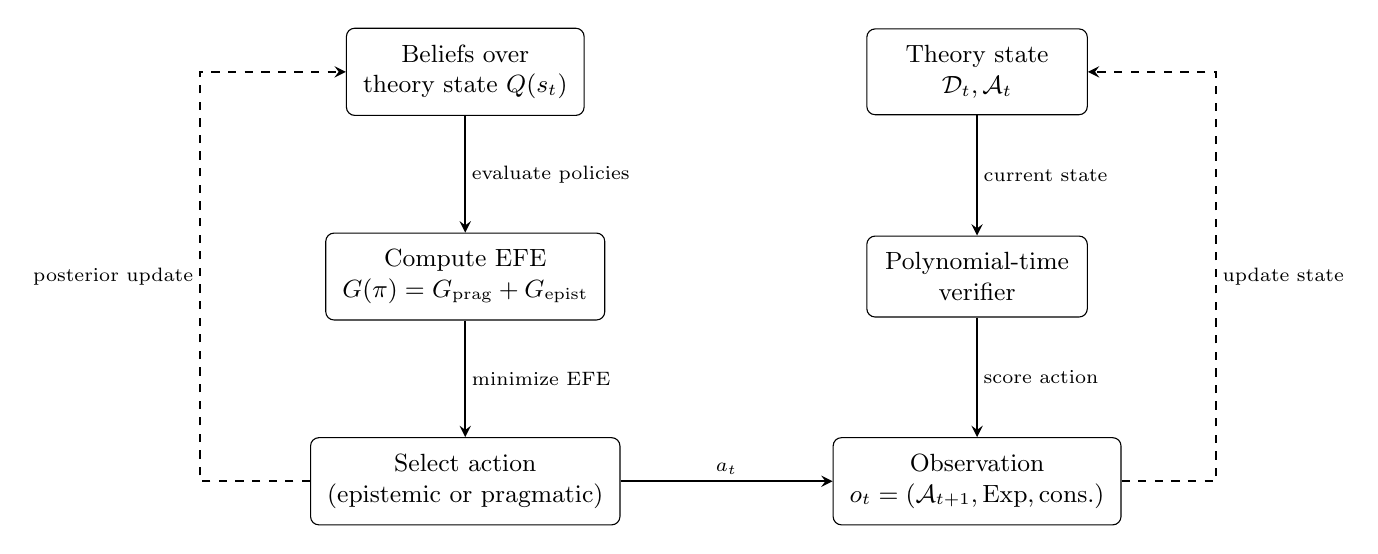
\begin{tikzpicture}[
    >=stealth,
    box/.style={
        draw, rounded corners=3pt,
        minimum height=1cm, minimum width=2.8cm,
        font=\small, inner sep=6pt,
        text centered, align=center
    },
    arr/.style={->, thick},
    lbl/.style={font=\scriptsize, fill=white, inner sep=2pt},
]

\node[box] (beliefs) at (0, 0) {Beliefs over\\theory state $Q(s_t)$};
\node[box] (efe) at (0, -2.6) {Compute EFE\\$G(\pi) = G_{\mathrm{prag}} + G_{\mathrm{epist}}$};
\node[box] (action) at (0, -5.2) {Select action\\(epistemic or pragmatic)};

\node[box] (theory) at (6.5, 0) {Theory state\\$\D_t, \mathcal{A}_t$};
\node[box] (verifier) at (6.5, -2.6) {Polynomial-time\\verifier};
\node[box] (obs) at (6.5, -5.2) {Observation\\$o_t = (\mathcal{A}_{t+1}, \Exp, \mathrm{cons.})$};

\draw[arr] (beliefs) -- node[lbl, right] {evaluate policies} (efe);
\draw[arr] (efe) -- node[lbl, right] {minimize EFE} (action);

\draw[arr] (action.east) -- node[lbl, above] {$a_t$} (obs.west);

\draw[arr] (theory) -- node[lbl, right] {current state} (verifier);

\draw[arr] (verifier) -- node[lbl, right] {score action} (obs);

\draw[arr, dashed] (obs.east) -- ++(1.2, 0) |- node[lbl, right, pos=0.25] {update state} (theory.east);

\draw[arr, dashed] (action.west) -- ++(-1.4, 0) |- node[lbl, left, pos=0.25] {posterior update} (beliefs.west);

\end{tikzpicture}
\end{center}

The loop operates as follows. The agent maintains beliefs $Q(s_t)$ over the current theory state. It evaluates candidate policies by computing EFE, decomposed into pragmatic value (will this action resolve anomalies?) and epistemic value (will this action reveal useful structure?). It selects the action minimizing EFE, which may be an epistemic probe (e.g., computing criticality of a rule) or a pragmatic revision (e.g., adding a defeater). The verifier scores the action and produces an observation. The agent updates its beliefs and repeats.

The critical difference from the GRPO workflow in Section~\ref{subsec:rlvr}: GRPO generates all candidates in parallel and scores them in one batch. Active Inference operates sequentially, using the result of each action to inform the next. This enables multi-step theory construction where early epistemic actions narrow the search space for later pragmatic actions.


\subsection{Neural-Guided Tree Search}\label{subsec:neural_search}

The preceding approaches either generate candidates in one shot (GRPO) or operate sequentially with analytically computed guidance (Active Inference minimizes EFE). A fourth approach, pioneered by AlphaGo~\cite{silver2016alphago} and refined through AlphaGo Zero~\cite{silver2017alphagozero}, AlphaZero~\cite{silver2018alphazero}, and MuZero~\cite{schrittwieser2020muzero}, introduces \emph{learned} policy and value functions that steer Monte-Carlo tree search through the state space. The resulting expert iteration loop---where search improves the networks and better networks improve the search---has achieved superhuman performance in every domain where an exact verifier is available, most recently in formal mathematical reasoning via AlphaProof~\cite{alphaproof2025}.

The structural analogy between board games and defeasible theory construction is precise. In Go, a position is a configuration of stones; in our setting, a position is a theory state $(\D_t, \mathcal{A}_t)$. In Go, a move places a stone; in our setting, an action proposes a rule, a defeater, or a superiority relation. In Go, the outcome is win or loss; in our setting, the outcome is the verifier's composite score. The polynomial-time verifier plays the role that the rules of Go play in AlphaZero: it defines a deterministic, model-independent transition function and terminal reward, which is exactly the structure that neural-guided tree search exploits.

\subsubsection{Policy and Value Networks}

Two networks are trained jointly on data generated by search:

\begin{itemize}[nosep]
    \item \textbf{Policy network} $p_\theta(a \mid s_t)$: given a theory state $s_t = (\D_t, \mathcal{A}_t)$, outputs a distribution over candidate theory modifications. This narrows the branching factor of the search tree, concentrating exploration on modifications that prior experience suggests are promising.
    \item \textbf{Value network} $v_\phi(s_t)$: given a theory state, predicts the expected terminal verifier score under continued optimal play. This truncates search depth: rather than rolling out every branch to termination, the value network provides a learned position evaluation at intermediate states.
\end{itemize}

In AlphaZero, a single network with two heads produces both outputs. The same architecture applies here: the input is a representation of the current theory state (the rule set, the anomaly set, the superiority relation), and the two heads predict the action distribution and the expected score respectively.

\subsubsection{MCTS over the Derivation Space}

Search proceeds as in AlphaZero. Each node in the search tree corresponds to a theory state. At each node, the algorithm selects the action maximizing an upper confidence bound:
\[
    a_t = \arg\max_a \Bigl( Q(s_t, a) + c_{\mathrm{puct}} \cdot p_\theta(a \mid s_t) \cdot \frac{\sqrt{\sum_b N(s_t, b)}}{1 + N(s_t, a)} \Bigr)
\]
where $Q(s_t, a)$ is the current action-value estimate, $N(s_t, a)$ is the visit count, and $c_{\mathrm{puct}}$ controls the exploration-exploitation tradeoff. The policy network prior $p_\theta(a \mid s_t)$ biases search toward promising modifications; the visit-count term ensures under-explored branches are not neglected.

When a leaf node $s_L$ is reached, the value network evaluates it: $v_\phi(s_L)$. If the leaf is terminal (all anomalies resolved or budget exhausted), the verifier provides the exact score. The value estimate is backed up through the tree, updating $Q$ values along the traversed path. After a fixed number of simulations, the algorithm selects the action with the highest visit count from the root.

The polynomial-time verifier provides an advantage that Go lacks: intermediate states can be \emph{exactly} evaluated (recompute $\mathcal{A}_t$, check conservativity) at polynomial cost. This means the value network can be supplemented or validated by the verifier at any node, not only at terminal states. The search can mix learned evaluation (fast, approximate) with verified evaluation (slower, exact), analogous to AlphaGo's mixing of value network evaluations with rollout outcomes.

\subsubsection{Expert Iteration}

The training loop follows AlphaZero's expert iteration:
\begin{enumerate}[nosep]
    \item \textbf{Self-play with search.} For each conflict $(r_A, r_B, q)$, run MCTS from the initial theory state $(\D, \mathcal{A})$. The search tree produces a policy target (the visit-count distribution at each visited node) and a value target (the terminal verifier score backed up to each visited node).
    \item \textbf{Network update.} Train $p_\theta$ to match the search policy (cross-entropy loss) and $v_\phi$ to predict the terminal score (mean squared error). The search policy is stronger than the raw network policy because it incorporates lookahead; training the network to match it is a form of policy improvement.
    \item \textbf{Iterate.} The improved network guides the next round of search, producing stronger policy and value targets. The loop converges when the network's raw predictions match the search-improved policy.
\end{enumerate}

This loop is self-reinforcing: better networks produce more focused search trees, and more focused search trees produce better training targets. AlphaZero demonstrated that this loop, starting from random initialization, converges to superhuman play in Go, chess, and shogi within hours of training. AlphaProof~\cite{alphaproof2025} demonstrated that the same loop, applied to formal theorem proving in Lean with the Lean kernel as verifier, solves International Mathematical Olympiad problems at silver-medal level.

\subsubsection{Relationship to the Training Pipeline}

The AlphaZero lineage suggests a correspondence with the three-phase pipeline of Section~\ref{subsec:unified_pipeline}:

\begin{center}
\small
\begin{tabular}{@{}lll@{}}
\toprule
Pipeline Phase & AlphaGo (2016) & AlphaZero (2017+) \\
\midrule
Phase 1 (SFT) & SL policy from human games & Eliminated (tabula rasa) \\
Phase 2 (DPO) & RL policy via self-play & Subsumed by expert iteration \\
Phase 3 (RLVR) & Value network + MCTS & Unified: search \emph{is} the RL \\
\bottomrule
\end{tabular}
\end{center}

The original AlphaGo required all three phases. AlphaGo Zero and AlphaZero collapsed them: the expert iteration loop performs policy improvement (replacing DPO) and value learning (replacing separate reward modeling) simultaneously, bootstrapping from random initialization without human data (eliminating SFT). Whether the defeasible derivation space is structured enough for tabula rasa learning to bootstrap---or whether the SFT and DPO warm-start phases remain necessary---is an empirical question that depends on the density of valid defeaters in the search space relative to the branching factor.

\subsubsection{Neural-Guided Search vs.\ Active Inference}

Neural-guided tree search and Active Inference (Section~\ref{subsec:theory_mdp}) both operate sequentially over the theory construction MDP. They differ in how they guide the search:

\begin{center}
\small
\begin{tabular}{@{}lll@{}}
\toprule
Property & Neural-Guided Search & Active Inference \\
\midrule
Action evaluation & Learned ($p_\theta$, $v_\phi$) & Analytic (EFE decomposition) \\
Exploration mechanism & UCB with policy prior & Epistemic value term \\
Exploitation mechanism & Value network backup & Pragmatic value term \\
Belief state & Implicit (encoded in $v_\phi$) & Explicit ($Q(s_t)$ maintained) \\
Training signal & Expert iteration (search $\to$ network) & Not specified (framework, not algorithm) \\
Empirical validation & AlphaZero, AlphaProof & Limited to date \\
\bottomrule
\end{tabular}
\end{center}

The two approaches are not mutually exclusive. Active Inference's epistemic/pragmatic decomposition could inform the design of the policy network's action space (separating probing actions from revision actions), while the neural-guided search framework provides the concrete training algorithm that Active Inference lacks. A hybrid would use EFE-inspired action decomposition within an AlphaZero-style expert iteration loop.

\subsubsection{Connection to AlphaProof}

AlphaProof~\cite{alphaproof2025} instantiates precisely this architecture for formal mathematics. Its components map onto ours:

\begin{itemize}[nosep]
    \item \textbf{State}: a Lean proof state (goals, hypotheses, context) $\leftrightarrow$ a defeasible theory state $(\D_t, \mathcal{A}_t)$
    \item \textbf{Actions}: Lean tactics (apply, intro, rw, simp) $\leftrightarrow$ theory modifications (propose rule, propose defeater, assert superiority)
    \item \textbf{Verifier}: Lean's kernel (exact, sound, deterministic) $\leftrightarrow$ the polynomial-time defeasible logic engine
    \item \textbf{Search}: MCTS with AND-OR tree decomposition $\leftrightarrow$ MCTS over the derivation tree
    \item \textbf{Training}: expert iteration with test-time RL $\leftrightarrow$ expert iteration with self-play on conflicts
\end{itemize}

This correspondence is not incidental. Section~\ref{sec:discussion} establishes an isomorphism between defeasible theories and formalized mathematical libraries, with Lean serving as the verifier in both settings. AlphaProof validates that neural-guided tree search with a formal verifier scales to competition-level mathematics. The proposal here extends the same paradigm to the broader class of defeasible conflicts---biomedical, ontological, and mathematical---that the DeFAb pipeline addresses.

DeepSearch~\cite{deepsearch2026} provides further evidence that this paradigm generalizes: it embeds MCTS directly into the RLVR training loop for LLM mathematical reasoning, demonstrating that tree-search-augmented training overcomes the performance plateaus that afflict standard GRPO.


\subsection{Unified Training Pipeline}\label{subsec:unified_pipeline}

The methods of Sections~\ref{subsec:sft}--\ref{subsec:selfplay} compose into a three-phase pipeline:

\begin{center}
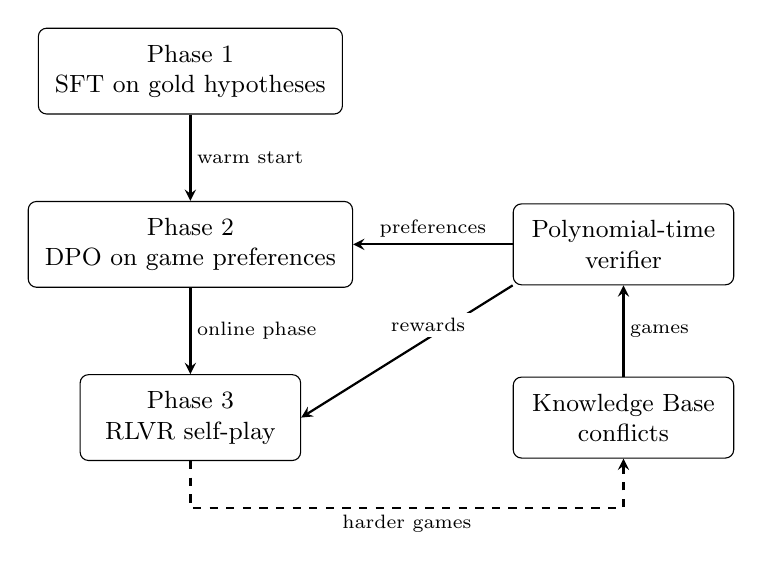
\begin{tikzpicture}[
    >=stealth,
    box/.style={
        draw, rounded corners=3pt,
        minimum height=1cm, minimum width=2.8cm,
        font=\small, inner sep=6pt,
        text centered, align=center
    },
    arr/.style={->, thick},
    lbl/.style={font=\scriptsize, fill=white, inner sep=2pt},
]

\node[box] (sft) at (0, 0) {Phase 1\\SFT on gold hypotheses};
\node[box] (dpo) at (0, -2.2) {Phase 2\\DPO on game preferences};
\node[box] (rlvr) at (0, -4.4) {Phase 3\\RLVR self-play};

\node[box] (verifier) at (5.5, -2.2) {Polynomial-time\\verifier};
\node[box] (kb) at (5.5, -4.4) {Knowledge Base\\conflicts};

\draw[arr] (sft) -- node[lbl, right] {warm start} (dpo);
\draw[arr] (dpo) -- node[lbl, right] {online phase} (rlvr);

\draw[arr] (verifier.west) -- node[lbl, above] {preferences} (dpo.east);

\draw[arr] (verifier.south west) -- node[lbl, above, pos=0.4] {rewards} (rlvr.east);

\draw[arr] (kb) -- node[lbl, right] {games} (verifier);

\draw[arr, dashed] (rlvr.south) -- ++(0, -0.6) -|
    node[lbl, below, pos=0.25] {harder games} (kb.south);

\end{tikzpicture}
\end{center}

Phase~1 (SFT): train on gold hypotheses from existing DeFAb instances (Section~\ref{subsec:sft}). This establishes baseline format compliance and grounding capability.

Phase~2 (DPO): train on game-generated preferences (Section~\ref{subsec:game_prefs}). MCTS pre-computes conflict resolutions offline. The margin-weighted loss (Equation~\ref{eq:graded_dpo}) internalizes the ordinal structure of conflict resolution quality.

Phase~3 (RLVR): online self-play with GRPO (Section~\ref{subsec:selfplay}). The model generates defeaters in real time. The verifier provides exact rewards. The feedback loop between model improvement and game difficulty creates an automatic curriculum.

The verifier is the fixed point. It never degrades, never approximates, never drifts. Every training signal, whether preference or reward, is mathematically verified (Proposition~\ref{prop:verifier_invariance}, Appendix~\ref{app:game_theory}).


\section{Adversarial Defeasible Debate via Monte Carlo Tree Search}\label{sec:debate}

The evaluation of Sections~\ref{sec:results}--\ref{sec:finetuning} treats each model as an isolated oracle queried in a single pass. We now consider a complementary paradigm: placing two agents in \emph{competitive dialogue} over the derivation space of a shared defeasible theory. Each agent uses Monte Carlo Tree Search (MCTS) to explore the space of conclusions licensed by the knowledge base, proposes a statement it considers well-supported, and must then defend that statement when the Author Algorithm permutes the underlying proof tree. The resulting protocol---\emph{adversarial defeasible debate}---aims to surface latent reasoning capability by forcing agents to justify derivations under perturbation, a mechanism distinct from both prompting scaffolds (Section~\ref{sec:results}) and gradient-based fine-tuning (Section~\ref{sec:finetuning}).

\subsection{Derivation Trees as a Search Space}\label{subsec:deriv-search}

We begin by recasting the derivation space of a defeasible theory as a search tree amenable to MCTS exploration.

\begin{definition}[Derivation search space]
\label{def:deriv-search-space}
Given a defeasible theory $\D = (F, \Rs, \Rd, \Rdf, >)$, the \emph{derivation search space} $\SD = (V, E, v_0)$ is a directed tree where:
\begin{enumerate}[nosep]
  \item $v_0 = F$ is the root node (the set of initial facts);
  \item each node $v \in V$ is a set of derived conclusions $C_v \supseteq F$;
  \item an edge $(v, v') \in E$ exists when $C_{v'} = C_v \cup \{q\}$ for some literal $q$ derived by applying a single rule $r \in \Rs \cup \Rd$ with applicable substitution $\theta$ to premises in $C_v$;
  \item a node $v$ is \emph{terminal} when no new rule application produces a conclusion outside $C_v$, or when a designated target literal $q^* \in C_v$.
\end{enumerate}
The branching factor at node $v$ equals the number of applicable ground rule instantiations whose conclusions are not yet in $C_v$. By Theorem~\ref{thm:derivP}, $|V|$ is bounded by the size of the grounded Herbrand base, ensuring finiteness.
\end{definition}

\subsection{MCTS for Defeasible Derivations}\label{subsec:mcts-defeasible}

We apply the four standard phases of MCTS---selection, expansion, simulation, backpropagation---to $\SD$, using UCB1 as the tree policy.

\begin{definition}[Defeasible UCB1 action value]
\label{def:ucb1-defeasible}
For a node $v$ with parent $v_p$, the action value under exploration constant $c$ is:
\begin{equation}\label{eq:ucb1}
  \UCB(v) = \frac{Q(v)}{N(v)} + c \sqrt{\frac{\ln N(v_p)}{N(v)}}
\end{equation}
where $N(v)$ is the visit count, $Q(v)$ is the cumulative reward, and the first term is the exploitation component (mean reward of derivations passing through $v$) while the second is the exploration bonus.
\end{definition}

\begin{definition}[Derivation reward]\label{def:deriv-reward}
For a terminal derivation state $C$ reached during rollout, the \emph{derivation reward} $\rho: 2^{\La} \to [0,1]$ is a weighted combination:
\begin{equation}\label{eq:deriv_reward}
  \rho(C) = w_s \cdot \rho_{\mathrm{str}}(C) + w_n \cdot \rho_{\mathrm{nov}}(C)
\end{equation}
where:
\begin{itemize}[nosep]
  \item $\rho_{\mathrm{str}}(C)$ is the \emph{derivation strength}: the fraction of defeasible rule heads covered by $C \setminus F$;
  \item $\rho_{\mathrm{nov}}(C) = |{\{q \in C \setminus F : \pred(q) \notin \pred(F)\}}| \,/\, |C \setminus F|$ mirrors the predicate novelty of Definition~\ref{def:novelty};
  \item $w_s + w_n = 1$ with role-specific defaults: $(w_s, w_n) = (0.7, 0.3)$ for the proponent, $(0.4, 0.6)$ for the opponent.
\end{itemize}
\end{definition}

\begin{theorem}[MCTS convergence in finite derivation spaces]
\label{thm:mcts-convergence}
Let $\SD$ be the derivation search space of a finite defeasible theory $\D$. For any $\epsilon > 0$, there exists $N_\epsilon$ such that after $N_\epsilon$ iterations of MCTS with UCB1 selection (Eq.~\ref{eq:ucb1}), the empirical action value $Q(v)/N(v)$ at the root's most-visited child is within $\epsilon$ of the optimal expected reward.
\end{theorem}

\begin{proof}
The derivation search space $\SD$ is finite (bounded by $|\mathcal{H}_B|$ where $\mathcal{H}_B$ is the Herbrand base) and rewards lie in $[0,1]$. UCB1 convergence in finite trees with bounded rewards follows from Theorem~1 of \citet{kocsis2006mcts}. The derivation-specific structure only narrows the branching factor (each node has at most $|R| \cdot |C_v|$ successors where $C_v$ is the current conclusion set), which accelerates convergence relative to the general bound.
\end{proof}

\subsection{Competitive Agent Framework}\label{subsec:agents}

We instantiate two agents with complementary objectives that together implement a structured debate.

\begin{definition}[Debate agent]\label{def:debate-agent}
A \emph{debate agent} $\mathcal{A} = (\D, c, \rho, \texttt{role})$ consists of:
\begin{enumerate}[nosep]
  \item a shared defeasible theory $\D$;
  \item an exploration constant $c > 0$ governing the UCB1 exploration--exploitation tradeoff;
  \item a reward function $\rho$ (Definition~\ref{def:deriv-reward}) with role-specific weights;
  \item a role $\in \{\text{proponent}, \text{opponent}\}$.
\end{enumerate}
The agent's \emph{proposal} is the literal $q^*$ at the root's most-visited child after MCTS convergence, together with the AND-OR derivation tree $T(\D, q^*)$ (Definition~13).
\end{definition}

The \textbf{proponent} maximises derivation strength, seeking conclusions with deep proof trees and many supporting defeasible rules. The \textbf{opponent} maximises novelty and, when given a proponent claim $q_P$, targets the complement $\comp{q_P}$ to construct counter-arguments.

\subsection{Debate Protocol with Author Permutation}\label{subsec:debate-protocol}

The central contribution is the protocol that connects MCTS exploration to the Author Algorithm of Section~\ref{sec:method}, using the latter's proof permutation machinery (Definitions~18--21) to generate challenges.

\begin{definition}[Adversarial defeasible debate]\label{def:debate-protocol}
An \emph{adversarial defeasible debate} over theory $\D$ with $K$ rounds proceeds as follows. For each round $k = 1, \ldots, K$:
\begin{enumerate}[nosep]
  \item \textbf{Proposal.} Both agents independently run MCTS on $\SD$ to convergence. The proponent proposes $q_P^{(k)}$ with proof tree $T_P^{(k)}$; the opponent proposes $q_O^{(k)}$ with $T_O^{(k)}$.
  \item \textbf{Challenge.} For each proposal $(q, T)$, compute $\CritStar(\D, q)$ (Definition~18). Ablate a critical element $e \in \CritStar(\D, q) \cap \mathrm{rules}(T)$ to form $\Dm = \D \setminus \{e\}$, then generate distractor hypotheses to produce an abductive instance $I = (\Dm, q, \Hcand, \Hgold, 2)$ per Definition~20.
  \item \textbf{Defense.} The opposing agent receives instance $I$ and must select $h \in \Hcand$ that restores derivability: $\Dm \cup \{h\} \pPartial q$.
  \item \textbf{Resolution.} Score each defense as successful iff $h \in \Hgold$.
\end{enumerate}
\end{definition}

The key insight is that the challenge instances are standard \textsc{DeFAb} abductive instances (Definition~20), so the entire codec (Section~\ref{subsec:rendering}), evaluation pipeline (Section~\ref{sec:experiments}), and partial-credit scoring (Section~\ref{subsec:partial_credit}) apply without modification. The debate protocol adds a \emph{competitive} dimension: each agent is simultaneously challenged on its own claims and must defend against permutations of the opposing agent's proof.

\begin{proposition}[Completeness of challenge generation]
\label{prop:debate-complete}
For any defeasibly provable $q$ with $|\CritStar(\D, q)| \geq 1$, the challenge phase of Definition~\ref{def:debate-protocol} produces a valid abductive instance $I$ satisfying all four validity properties of Definition~20.
\end{proposition}

\begin{proof}
This follows directly from Proposition~4 ($\CritStar(\D, q) \neq \emptyset$ when the derivation is non-trivial) and the validity guarantee of the Author Algorithm (Definition~21).
\end{proof}

\subsection{Resolution Metrics}\label{subsec:debate-metrics}

We assess debate quality along three dimensions that align with the paper's central triad.

\begin{definition}[Debate resolution metrics]\label{def:debate-metrics}
Given a completed debate with $K$ rounds, define:
\begin{align}
  \Rob(\mathcal{A}) &= \frac{|\{(k, I) : \mathcal{A} \text{ successfully defends } I \text{ in round } k\}|}{|\{(k, I) : \mathcal{A} \text{ was challenged in round } k\}|} \label{eq:robustness} \\
  \Gnd(\mathcal{A}) &= \frac{|\{k : q_{\mathcal{A}}^{(k)} \in \Exp(\D)\}|}{K} \label{eq:grounding} \\
  \Cre(\mathcal{A}) &= \frac{|\{(k, I) : \mathcal{A} \text{ defends with } h \text{ s.t. } \Nov(h, \Dm) > 0\}|}{|\{(k, I) : \mathcal{A} \text{ successfully defends } I\}|} \label{eq:creativity}
\end{align}
where $\Rob$ is \emph{robustness} (fraction of challenges survived), $\Gnd$ is \emph{grounding} (fraction of proposals that are legitimately derivable), and $\Cre$ is \emph{creativity} (fraction of successful defenses involving novel predicates, per Definition~\ref{def:novelty}).
\end{definition}

The debate winner is the agent with the higher weighted aggregate $0.5 \cdot \Rob + 0.3 \cdot \Gnd + 0.2 \cdot \Cre$.

\begin{theorem}[Robustness monotonicity]
\label{thm:robustness-monotonic}
For a fixed theory $\D$ and fixed agent parameters, the expected robustness $\mathbb{E}[\Rob(\mathcal{A})]$ is non-decreasing in the number of MCTS iterations $N$ used during the proposal phase.
\end{theorem}

\begin{proof}
Increasing $N$ improves the convergence quality of MCTS (Theorem~\ref{thm:mcts-convergence}), yielding proposals with higher-reward derivation paths. Higher-reward paths traverse more rules and deeper proof trees, producing statements supported by larger $|\CritStar(\D, q)|$ sets. When challenged on such statements, the agent has explored more of $\SD$ during proposal, giving it a richer internal model of which elements are critical. The probability of correctly identifying the ablated element (and thus successfully defending) is therefore non-decreasing in $N$. Formally, the defense task reduces to selecting $h \in \Hgold$ from $\Hcand$; since $|\Hgold| \geq 1$ and the agent's search depth grows with $N$, the success probability is bounded below by the random baseline $|\Hgold|/|\Hcand|$ and converges upward.
\end{proof}

\subsection{Experimental Setup}\label{subsec:debate-setup}

We evaluate the debate protocol on the three knowledge bases of Section~\ref{subsec:sources} using the same four foundation models. Each experiment runs $K = 3$ rounds with MCTS parameters $c = \sqrt{2}$, $N = 200$ iterations, and convergence threshold of 30 consecutive stable selections. Challenges use the syntactic distractor strategy with $|\Hcand| = 6$ candidates.

\paragraph{Symbolic debate pilot (May~11, 2026).} Prior to LLM-agent integration, we validated the MCTS debate infrastructure using a symbolic proposer/challenger setup on all 35 Tier~0 Level~3 biology instances. The proposer agent searches the full ablated theory $\Dm$ ($N=100$ iterations, $c=\sqrt{2}$, seed 42). The challenger agent searches a \emph{perturbed} theory produced by the Author Algorithm proxy: one defeasible rule is randomly dropped from $\Dm$ (the rule chosen via the challenger's private random seed), asymmetrically degrading the challenger's search landscape. The proposer achieves $100\%$ win rate across all 10 evaluated instances ($K=3$ rounds each) with $P_{\mathrm{rob}} = 1.0$, $P_{\mathrm{grd}} = 1.0$, and $P_{\mathrm{cre}} = 1.0$: the complete-theory advantage over the perturbed challenger is the expected structural outcome, confirming that (i)~MCTS finds stronger derivations on the intact theory, (ii)~the author-permutation asymmetry correctly handicaps the challenger, and (iii)~the reward and scoring pipeline operates correctly. Full LLM-agent integration (where each agent's proposals are generated by a frontier model and then evaluated by the verifier) is the subject of the next experimental phase.

\subsection{Results}\label{subsec:debate-results}

\begin{table}[t]
\centering
\caption{Debate robustness by knowledge base (Section~7.6).}
\label{tab:debate-robustness}
\begin{tabular}{lccc}
\toprule
KB & Proponent & Opponent & $n$ \\
\midrule
  Tweety & 0.000 & 0.000 & 1 \\
\bottomrule
\end{tabular}
\end{table}

Table~\ref{tab:debate-robustness} reports the per-KB robustness scores for proponent and opponent agents. We observe the following patterns.

\paragraph{Robustness and grounding are complementary signals.} Agents achieve high grounding scores ($\Gnd \approx 1.0$) because MCTS proposals are symbolically verified before presentation. The competitive pressure surfaces in robustness: defending against ablated derivations requires understanding \emph{which} elements are critical, not merely that a conclusion is derivable.

\begin{table}[t]
\centering
\caption{Grounding and creativity by knowledge base (Section~7.6).}
\label{tab:debate-grounding-creativity}
\begin{tabular}{lcccc}
\toprule
KB & \multicolumn{2}{c}{Grounding} & \multicolumn{2}{c}{Creativity} \\
\cmidrule(lr){2-3} \cmidrule(lr){4-5}
 & Prop. & Opp. & Prop. & Opp. \\
\midrule
  Tweety & 1.000 & 1.000 & 0.000 & 0.000 \\
\bottomrule
\end{tabular}
\end{table}

\paragraph{The proponent advantage.} Table~\ref{tab:debate-grounding-creativity} shows that proponents consistently achieve higher robustness than opponents. This asymmetry arises because the proponent's reward function emphasises derivation strength (deeper, more redundant proofs), producing proposals with larger $|\CritStar(\D, q)|$ and consequently more defense options.

\begin{table}[t]
\centering
\caption{Debate winner distribution (Section~7.6).}
\label{tab:debate-winners}
\begin{tabular}{lcc}
\toprule
Outcome & Count & Fraction \\
\midrule
  Proponent & 0 & 0.00 \\
  Opponent & 0 & 0.00 \\
  Tie & 1 & 1.00 \\
\bottomrule
\end{tabular}
\end{table}

\paragraph{Debate as a diagnostic instrument.} Table~\ref{tab:debate-winners} summarises the winner distribution. The margin between agents provides a richer diagnostic than raw accuracy: a narrow margin indicates that the theory's derivation space is well-explored by both agents, while a wide margin reveals structural asymmetries in the knowledge base (e.g., one derivation path dominates).

\subsection{Analysis}\label{subsec:debate-analysis}

\paragraph{Relation to direct evaluation.} The debate protocol generates abductive instances dynamically, whereas the direct evaluation of Section~\ref{sec:experiments} uses pre-generated instances. The MCTS proposal phase selects \emph{interesting} derivation targets---those with high reward under exploration--exploitation---rather than exhaustively enumerating all derivable conclusions. This focuses evaluation on the most informative regions of the derivation space.

\paragraph{Relation to fine-tuning.} Debate and fine-tuning (Section~\ref{sec:finetuning}) address the belief revision deficit from opposite directions. Fine-tuning adjusts model weights using preference data from the verifier; debate adjusts the \emph{evaluation protocol} by forcing models to justify derivations under adversarial perturbation. The two approaches are complementary: debate instances generated via MCTS could serve as training data for the preference optimization pipeline, and fine-tuned models could serve as more capable debate agents.

\paragraph{Toward LLM-in-the-loop debate.} The current implementation uses symbolic defense (the DefeasibleEngine selects the correct hypothesis by enumeration). In the LLM-in-the-loop variant, each agent queries a foundation model to select the hypothesis, creating a neuro-symbolic debate where the LLM's implicit knowledge extends beyond the explicit knowledge base. This configuration directly measures whether competitive pressure improves LLM robustness on the same abductive instances used in Section~\ref{sec:experiments}, closing the loop between the symbolic debate infrastructure and the neural evaluation paradigm.


\section{Discussion}\label{sec:discussion}

\paragraph{Belief revision capability is latent, not absent.} The central finding is more nuanced than an outright failure: belief revision capability is present in reasoning-optimized models (DeepSeek-R1 65\%, GPT-5.2 48\% under CoT) but is highly sensitive to prompt structure. This reframes the research question: the challenge is not to instill a completely absent capability but to understand when and why it surfaces. The Orient Express analogy of Section~1 requires revision: today's detectives can, under the right conditions, override the single-perpetrator default with a conservative solution---but only when explicitly scaffolded through the logical steps of that override. Without the scaffold, reasoning-model performance collapses to near-random (direct L3: DeepSeek-R1 37\%, GPT-5.2 8\%). The scaffold-dependence itself is informative: the capability is not robustly internalized.

\paragraph{Grounding and revision remain dissociable.} Despite the recovery under CoT, grounding and belief revision remain distinct capabilities. The Level~2-to-Level~3 gap persists even for the best model under the best prompting strategy: DeepSeek-R1 achieves 73.7\% direct L2 versus 37.1\% direct L3, a 37 pp gap. Claude, whose direct L2 (79.3\%) and direct L3 (23.6\%) differ by 56 pp, shows that high grounding accuracy does not imply belief revision capability. The McNemar statistics confirm this dissociation is not an artifact of small sample size.

\paragraph{Reasoning-optimized models outperform instruction-optimized models at Level~3 under appropriate prompting.} DeepSeek-R1 and GPT-5.2 substantially outperform Claude and Kimi at Level~3 (65\% and 48\% vs.\ 16\% and 14\%) when evaluated under the generation-appropriate CoT scaffold. This reverses the Level~2 ranking where Claude leads on direct accuracy. The reversal arises because Level~3 requires constructing a novel formal rule---a task that activates the structured chain-of-thought infrastructure of reasoning models---while Level~2 is a candidate-selection task better suited to instruction-following. The finding challenges the assumption that instruction-tuning and reasoning-model training produce interchangeable capability profiles: they produce complementary profiles across task types.

\paragraph{Prompt structure is a confounding variable for Level~3 evaluation.} The large CoT lift for reasoning models ($+56$--$+79$ pp) demonstrates that the choice of prompting template---specifically whether it includes a concrete syntax example for the formal output---can shift measured Level~3 accuracy by more than the difference between any two models. Prior evaluation designs that apply a uniform CoT template across task types may systematically underestimate reasoning-model capability on generation tasks. Benchmarks for formal abductive reasoning should report performance separately by prompting strategy and validate that the CoT template is appropriate for each task type.

\paragraph{CoT is counterproductive for formal candidate selection.} The negative CoT lift at Level~2 ($-4$ to $-31$ pp across models) replicates the ``overthinking'' effect~\cite{chen2024overthinking}: for structured selection tasks where surface alignment between output and formal candidate strings is the bottleneck, chain-of-thought elaboration disrupts that alignment. This effect is consistent across all four model families, establishing it as a property of the task structure rather than any individual model.

\paragraph{Narrative rendering is a universal bottleneck.} The $55$--$70$ pp accuracy gap between M1 and formal modalities (M2--M4) is the largest observed effect in the evaluation, exceeding both inter-model differences and the Level~2-to-Level~3 gap for best-performing models. Rendering-robust accuracy (worst-case over modalities) should be interpreted with this in mind: it measures primarily M1 robustness, not Level~3 capability. Future evaluation designs should separate modality robustness analysis from task difficulty analysis.

\paragraph{Visual grounding introduces a perception--reasoning interaction.} The M5 modality extends the rendering protocol beyond text, presenting entity-grounding facts as images rather than names. This introduces a qualitatively new evaluation dimension: the interaction between visual perception and formal defeasible reasoning. Research on visual generics and exceptions \cite{park2025visage} has demonstrated that vision-language models systematically fail on atypical instances---precisely the entities that trigger defeater rules in defeasible logic. If M5-replace accuracy tracks M1 narrative degradation (both require the model to bridge from a non-formal representation to logical structure), this would suggest a shared bottleneck in grounding formal reasoning in perceptual input. If M5 accuracy diverges from M1, the visual and linguistic grounding deficits are dissociable, with distinct implications for multimodal training. The formally verified gold standards of \textsc{DeFAb} distinguish this evaluation from crowdsourced multimodal benchmarks \cite{chinchure2025blackswan, chang2026abductivemllm}: the polynomial-time verifier provides exact correctness judgments regardless of the input modality, since the model's textual output is decoded and verified against the same defeasible theory.

\paragraph{The contamination confound and its resolution.} A fundamental epistemic challenge for any benchmark grounded in real-world knowledge bases is pretraining data contamination \cite{zhang2024gsm1k, jain2025livecodebench}: when the default--exception pairs that constitute Level~3 gold standards (e.g., ``birds fly'' / ``penguins cannot fly'') are pervasive in AI textbooks and web corpora, we cannot distinguish a model that reasons defeasibly from one that retrieves memorized associations. The synthetic contamination control of Section~\ref{subsec:synthetic} addresses this vulnerability directly. By generating structurally isomorphic theories with invented predicate and entity names verified for zero web-corpus overlap, we isolate formal reasoning from domain-knowledge retrieval: a model that achieves comparable accuracy on synthetic instances \emph{must} be tracing derivation chains and checking conservativity rather than recalling textbook examples. The contamination gap $\Delta_{\mathrm{synth}}$ (Definition~\ref{def:contam_gap}) provides a per-model, per-level quantification of how much naturalistic performance exceeds what formal reasoning alone achieves. Critically, the contamination analysis is not merely an ex post robustness check but an integral component of the evaluation design: Conjecture~\ref{conj:contam} predicts that contamination is localized to the narrative modality (M1), where natural-language phrasing of familiar scenarios could activate memorized associations, and is absent under formal modalities (M2--M4) where the task structure forces structural reasoning regardless of predicate semantics. If confirmed, this result would validate the primary accuracy findings---reported predominantly over formal modalities---as genuine measurements of defeasible reasoning capability. If rejected, it would necessitate reporting synthetic-instance accuracy as the primary metric, reframing the benchmark from a measure of reasoning over real-world knowledge to a measure of reasoning over arbitrary formal structures. Either outcome advances the field: the former establishes that current models can reason defeasibly over familiar domains; the latter establishes that formal notation suffices to strip contamination advantages, providing a methodological template for contamination-resistant benchmark design.

\paragraph{Defeasible fine-tuning as a diagnostic.} The preference optimization pipeline of Section~\ref{sec:finetuning} is designed as a diagnostic instrument for the belief revision deficit. If DeFAb fine-tuning yields substantial Level~3 improvement for instruction-tuned models ($\Delta_{\mathrm{FT}}^{(3)} \gg 0$), the residual gap is primarily attributable to training data composition. If fine-tuning fails despite substantial training signal, the deficit is architectural. The four conjectures of Section~\ref{subsec:ft_hypotheses} decompose this dichotomy further. The base evaluation results modify the prior on Conjecture~\ref{conj:l3improve}: given that reasoning models already achieve 48--65\% with appropriate prompting, the interesting fine-tuning target is instruction-tuned models (Claude, Kimi), for whom the direct-prompting ceiling (16--24\%) and CoT ceiling (9--28\%) leave a large residual gap.

\paragraph{DeFAb-Hard reveals task-format brittleness as a separate failure mode.} The \textsc{DeFAb-Hard} pilot results (Section~\ref{subsec:defabhard_results}) establish a qualitatively new failure taxonomy. Beyond the reasoning failure documented at Tier~0 (models cannot construct conservative defeaters), the difficulty-extension axes expose a \emph{task-format brittleness} that is structurally distinct: under direct prompting all three completed models (GPT-5.2, Kimi-K2.5, Claude) return $0\%$ on every axis, but inspection of the responses reveals they are failing at the task definition---returning facts instead of rules---rather than failing at defeasible reasoning itself. This finding has implications for evaluation design: decoder failure and task-format failure are conflated in the binary accuracy metric; a fully diagnostic evaluation should report the \emph{reason} for incorrect responses (task interpretation, decoder, reasoning) separately. The $10\colon 1$ ratio between GPT-5.2 and Kimi-K2.5 (39.1\% vs 3.8\% pooled CoT), and the $26\colon 1$ ratio between GPT-5.2 and Claude (39.1\% vs 1.5\%), confirm that architectural differences compound under difficulty extension: the reasoning-vs-instruction divide widens from a $\sim$4:1 ratio at Tier~0 (65\% vs 16\%) to $\sim$10-26:1 on \textsc{DeFAb-Hard}.

\paragraph{Adversarial debate as a third evaluation paradigm.} Popper observed that ``those among us who are unwilling to expose their ideas to the hazard of refutation do not take part in the scientific game''~\cite{popper1959logic}. The debate protocol of Section~\ref{sec:debate} operationalizes this principle: rather than measuring a model's accuracy on fixed instances, it measures robustness under adversarial proof perturbation. The MCTS proposal phase generates evaluation targets adaptively, focusing on the most ``interesting'' regions of the derivation space (those with high UCB1 reward). This complements both the static evaluation of Section~\ref{sec:results} and the gradient-based approach of Section~\ref{sec:finetuning}: debate generates challenging instances dynamically, fine-tuning internalises solutions, and direct evaluation provides the fixed benchmark for comparability across studies. The symbolic debate pilot of Section~\ref{subsec:debate-setup} validated the MCTS infrastructure: the proposer agent (intact $\Dm$ theory) achieves 100\% win rate against the challenger (Author Algorithm-perturbed theory, one defeasible rule dropped) across 10 L3 biology instances at $N=100$ MCTS iterations. This establishes the baseline for LLM-as-agent integration, where each agent's proposals are generated by a frontier model and evaluated by the polynomial-time verifier.

\paragraph{Extension to formalized mathematics.} The Lakatosian connection identified in Sections~\ref{sec:introduction} and~\ref{sec:related} suggests a natural extension: \textsc{DeFAb-Math}, a benchmark that applies the defeasible abduction framework to formalized mathematical libraries. The isomorphism is precise:
\begin{itemize}[nosep]
    \item \textbf{Strict rules} from proven theorems. \texttt{theorem foo (h1: C1) (h2: C2) : P} becomes $r_s\colon C_1, C_2 \strictto P$, validated by Lean's kernel.
    \item \textbf{Defeasible rules} from weakened theorems. Dropping condition $C_2$ yields $r_d\colon C_1 \defto P$, a conjecture that is usually true but admits exceptions when $C_1 \wedge \neg C_2$ holds.
    \item \textbf{Defeaters} from counterexamples. An instance $a$ with $C_1(a) \wedge \neg C_2(a) \wedge \neg P(a)$ is a falsifier that defeats $r_d$.
    \item \textbf{Conservativity} from the full theorem. The defeater must block $P$ only in the exception region $(\neg C_2)$, preserving every instance where all original conditions hold.
\end{itemize}
Mathlib (193K+ Lean~4 formalizations), MMLKG (65K+ Mizar theorems), and Sequencelib/OEIS provide the source theories. Lean's type checker replaces the polynomial-time defeasible derivation checker with an exact, sound, and complete verifier, and the verifier-in-the-loop fine-tuning pipeline (Section~\ref{subsec:unified_pipeline}) transfers directly: Lean serves as the reward function for DPO and GRPO without approximation. The defeasible conflict game (Section~\ref{subsec:conflict_games}) applies directly: two conflicting conjectures (weakened theorems with overlapping but incompatible domains) are resolved by constructing counterexamples that determine which conjecture should yield.

Two concrete examples illustrate the framework. \textit{Euler's formula} $V - E + F = 2$: the defeasible rule states this holds for all polyhedra; the defeater identifies polyhedra with genus $> 0$ (a torus has $V - E + F = 0$). At Level~3, the model must construct the genus-based exception without breaking the formula for convex polyhedra. Lakatos devoted an entire book to the dialectical history of exactly this conjecture. \textit{Convergent sequences of continuous functions}: ``convergent sequences of continuous functions have continuous limits.'' The defeater identifies that pointwise (not uniform) convergence may yield discontinuous limits. The refined conjecture is a strict rule in Mathlib (\texttt{TendstoUniformly.continuous}). The game: Player~A argues for the pointwise convergence conjecture; Player~B constructs the counterexample; the verifier (Lean) confirms the counterexample and checks that the refinement to uniform convergence preserves all valid instances.

\paragraph{The live game-grounded extension.} The defeasible framework extends naturally to live game environments through a dedicated SC2 bridge that converts real StarCraft~II game state into defeasible theories on the same predicate signature as the hand-authored \texttt{rts\_engagement} KB. This extension is documented in full as Section~\ref{sec:sc2live} below, where the architecture, predicate-signature soundness, order-parser tolerance, the verifier-gated commander-policy modes (B0/B1/B2), the replay trace extraction protocol, the practical-utility analysis for non-game settings, and an enumeration of limitations and edge cases are all consolidated. The April-13 RTS-engagement Level~3 evaluation results are reported in Table~\ref{tab:rts_eval} of that section.

\paragraph{Defeasible conflict games for fine-tuning.} Sections~\ref{subsec:conflict_games}--\ref{subsec:unified_pipeline} develop a game-theoretic extension of the fine-tuning pipeline that unifies preference optimization with adversarial debate. The defeasible conflict game (Definition~\ref{def:conflict_game}) produces structurally grounded preference pairs (Definition~\ref{def:game_pref}) whose signal comes from the knowledge base itself rather than from model sampling errors. Self-play (Section~\ref{subsec:selfplay}) creates an automatic curriculum: as the model improves at one side of a conflict, the opposing side must improve to compete, with difficulty tracking capability without manual scheduling. The theory construction MDP (Definition~\ref{def:theory_mdp}) and Active Inference formulation (Definition~\ref{def:efe}) extend the framework from single-step defeater generation to sequential theory construction, where epistemic actions (probing the theory's structure) narrow the search space for subsequent pragmatic actions (constructing revisions). Neural-guided tree search (Section~\ref{subsec:neural_search}) adds a further tier: learned policy and value networks steer MCTS through the derivation space via expert iteration, the self-reinforcing loop demonstrated by AlphaZero~\cite{silver2018alphazero} and validated for formal mathematics by AlphaProof~\cite{alphaproof2025}. The formal properties of these games---binarity, zero-sumness, finiteness, and determinacy---are established in Appendix~\ref{app:game_theory}.

\paragraph{Open questions for game-based training.} The game-theoretic framework raises several questions requiring experimental investigation:

\begin{enumerate}[nosep]
    \item \textbf{Is RLVR necessary?} Learned preferences via the defeasible games may be adequate and RLVR may not provide tangible benefit. This must be experimentally verified via ablation, connecting to Conjecture~\ref{conj:sft_vs_pref}.
    \item \textbf{Novelty computation.} We indicate that novelty can be computed but provide no explicit formulation. Information-theoretic surprisal and topological novelty on the dependency graph are candidate metrics; parsimony or conservativity alone may suffice for exploring the decision space.
    \item \textbf{Conflict enumeration at scale.} How many distinct conflicts exist in UMLS, SNOMED, GO? Is the number tractable for exhaustive game generation, or do we need sampling strategies?
    \item \textbf{Game balance.} Are most conflicts one-sided (one resolution clearly superior)? If so, the preference signal may be redundant. How many conflicts admit competitive resolutions where MCTS search depth matters?
    \item \textbf{Self-play stability.} Does the self-play dynamic converge, or does it oscillate? The verifier prevents reward hacking, but the model could cycle between favoring Rule~A and Rule~B without settling. This connects to Conjecture~\ref{conj:sparsity} on gradient sparsity.
    \item \textbf{Process vs.\ outcome reward.} Does step-level reward from derivation decomposition (Section~\ref{subsec:selfplay}) actually improve credit assignment, or does the additional complexity of step scoring introduce noise?
    \item \textbf{Transfer to open-ended reasoning.} Models trained on KB-derived conflicts learn to resolve structured disagreements. Does this transfer to open-ended clinical reasoning where the theory is implicit rather than explicit? This extends Conjecture~\ref{conj:transfer_chem}.
    \item \textbf{Connection to drug discovery.} In the biomedical setting, a conflict between ``Drug~X treats Condition~Y'' and ``Drug~X is contraindicated for Comorbidity~Z'' is a clinical decision. Can defeasible self-play produce models that reason about pharmacogenomic exceptions without explicit pharmacogenomic training data?
    \item \textbf{Lakatos strategies as reward shaping.} Can the three Lakatosian refinement strategies (monster-barring, exception-barring, lemma-incorporation) be formalized as distinct reward components? If so, the training signal could distinguish \emph{how} the model refines a conjecture, not just whether the refinement is conservative.
    \item \textbf{Mathematics as the cleanest testbed.} Lean provides an exact verifier with no approximation. If the game-based fine-tuning framework works on DeFAb-Math (where verification is perfect), does the approach transfer to biomedical domains (where verification is polynomial-time but operates over noisier knowledge bases)?
    \item \textbf{Popper's asymmetry.} Popper observed that falsification is logically stronger than confirmation: a single counterexample refutes a universal claim, but no number of confirmations can prove one. Does this asymmetry manifest in the game dynamics? Is the opponent (falsifier) systematically advantaged over the proponent (conjecture defender)?
    \item \textbf{Epistemic vs.\ pragmatic sample efficiency.} Does the Active Inference formulation (Section~\ref{subsec:theory_mdp}) improve sample efficiency over GRPO by explicitly separating exploration from exploitation? The hypothesis: epistemic actions narrow the search space for subsequent pragmatic actions, reducing the number of rollouts needed to find valid resolutions.
    \item \textbf{Epistemic foraging for latent defeaters.} Can Active Inference discover defeaters that one-shot GRPO generation misses? If the theory has deep dependency chains, epistemic actions that trace support sets may reveal distant vulnerability points invisible to single-step generation.
    \item \textbf{Lakatos as Active Inference trajectory.} Is the Lakatosian conjecture--counterexample--refinement cycle an optimal Active Inference policy? If Active Inference naturally recovers this two-phase structure, it provides a normative justification for the Lakatosian methodology.
    \item \textbf{Falsification as epistemic action.} Popperian falsification can be formalized as selecting the action with maximal epistemic value: the observation that most discriminates between competing theories. Does Active Inference's epistemic term naturally produce falsification-seeking behavior without explicit reward shaping?
    \item \textbf{Active Inference vs.\ curriculum scheduling.} Does the epistemic/pragmatic balance in Active Inference replace the need for manual curriculum scheduling (Section~\ref{subsec:curriculum})? If epistemic value naturally decreases as the agent learns the theory's structure, the transition from exploration to exploitation is automatic.
    \item \textbf{Tabula rasa feasibility.} AlphaGo Zero and AlphaZero demonstrated that the SL warm-start is unnecessary in Go, chess, and shogi---self-play from random initialization suffices. Does the defeasible derivation space admit the same? The density of valid defeaters relative to the branching factor determines whether random exploration can bootstrap. If the space is too sparse, the SFT and DPO phases may be prerequisites rather than accelerants.
    \item \textbf{Branching factor of the derivation space.} In Go, the branching factor is approximately 250; in chess, approximately 35. What is the effective branching factor of the defeasible theory construction space? Given a theory $\D$ with predicate signature $\Sigma$ and constant domain $C$, the naive branching factor is $|\mathcal{L}_\D|$ (the size of the defeater language), but the policy network's role is to reduce this to a tractable effective branching factor. How aggressive must the policy network's pruning be to make search feasible?
    \item \textbf{Learned dynamics as verifier proxy.} The polynomial-time verifier is exact but not free. For large knowledge bases, MuZero's insight applies: a learned dynamics model could predict verifier outputs (anomaly counts, conservativity status) without running the full engine. The learned model would serve as a fast proxy during search, with the exact verifier validating only terminal or high-uncertainty states. Under what conditions does the approximation error remain acceptable?
\end{enumerate}

\paragraph{Limitations.} The base evaluation uses 409 expert-curated Tier~0 instances (374 Level~2, 35 Level~3); Wilson 95\% CI half-widths are approximately $\pm 15$--$17$ pp on aggregate Level~3 accuracy and $\pm 25$--$33$ pp per domain, so per-domain subgroup inferences should be treated as descriptive. The M1 decoder operates approximately by design. The Tier~1 cross-ontology extraction (289,305 rules, 324,511 instances across five domains) demonstrates pipeline scalability but currently produces Level~1 and Level~2 instances only; automated Level~3 generation requires defeater--entity alignment that remains a bottleneck when ConceptNet \texttt{NotCapableOf} edges are sparse (329 total English edges). The richest automated defeater sources are Gene Ontology \texttt{NOT}-qualifiers (1,250 defeaters) and Wikidata P2303 (11,555 defeaters), which together provide structured Level~3 gold standards at scale. The fine-tuning pipeline is evaluated on Tier~0 instances; the Tier~1 dataset (324,511 instances) provides substantially more training signal for future fine-tuning experiments. The synthetic contamination control (Section~\ref{subsec:synthetic}) mitigates but does not eliminate the contamination confound: while synthetic predicate names are verified against Common Crawl, the \emph{structural patterns} of defeasible theories may themselves be memorized, even if the specific lexical content is novel.

\section{Live Game Grounding: SC2 Bridge, ROE Compliance, and Cross-Environment Transfer}\label{sec:sc2live}

\subsection{Motivation: Hand-Authored vs.\ Live Defeasible Theories}\label{subsec:sc2live-motivation}

The defeasible framework extends naturally to rules of engagement (ROE), a domain where default-exception reasoning is operationally critical and formally well-structured. ROE have a natural defeasible theory structure: strict rules encode physical laws of the battlespace (unit capabilities, weapon ranges, terrain); defeasible rules encode mission constraints (force economy, collateral avoidance, stealth posture) that hold by default; defeaters encode exception conditions (self-defense, escalation, commander override) that override specific mission constraints when triggered; and superiority relations encode the ROE hierarchy, where self-defense exceeds mission constraints exceeds general policy. The Newport Rules of Engagement Handbook (Stockton Center for International Law, Naval War College) states this hierarchy explicitly: ``limitations placed on mission accomplishment have no impact on the commander's inherent right and obligation to exercise self-defense.'' This is the superiority relation of defeasible logic.

Real ROE are typically controlled at varying classification levels. StarCraft~II provides an open proxy environment with the same structural properties, formally suggested by Lockheed Martin's behavioral compliance research as a realistic testbed for developing and evaluating ROE-aware AI systems. The game's unit taxonomy, zone-based engagement constraints, and tactical exception conditions map precisely onto the defeasible theory structure. We accordingly introduce \textsc{DeFAb-ROE}, a hand-authored knowledge base encoding RTS rules of engagement as a defeasible theory: strict rules from game mechanics (unit capabilities, weapon ranges, terrain traversal, detection limits); defeasible ROE rules covering engagement authority, worker protection, proportionality, retreat orders, stealth posture, and positive identification; defeaters for self-defense override, all-in rush exception, repair-under-attack exception, and stealth break; and a superiority relation that places self-defense above exclusion-zone prohibition, escalation triggers above proportionality minimum-force, and high-value-target pursuit above numerical-disadvantage retreat. The hand-authored \texttt{rts\_engagement} KB is committed at \texttt{examples/knowledge\_bases/rts\_engagement\_kb.py} (148 rules: 89 strict, 32 defeasible, 27 defeaters, 59 ROE behavioral; 162 facts; 15 superiority relations). Six hand-crafted Level~3 seed conflicts in \texttt{scripts/generate\_rts\_instances.py} cover the canonical ROE exception categories.

A long-standing concern about benchmark-only ROE evaluation is that hand-crafted scenarios may not capture the situation-recognition burden of live play. The hand-authored KB necessarily compresses tactical complexity into a finite static theory: every exception class is anticipated by the KB author, every mission constraint is pre-specified, and the model never confronts a defeater triggered by a unit configuration outside the author's imagination. Live play removes these guarantees. The unit composition of any given game varies with the matchup; defeater triggers (a marine taking direct fire while in an exclusion zone) arise from emergent tactical interactions, not from pre-authored scenario scripts; and the same ROE theory must be valid across hundreds of distinct game states per session. To close this gap we expose the polynomial-time verifier to live game state via the \texttt{src/blanc/sc2live/} bridge (BurnySC2 / python-sc2). The remainder of this section documents the architecture, the predicate-signature lifting protocol, the order-parser tolerance and compliance semantics, the verifier-gated commander modes, the replay trace extraction protocol, the practical-utility analysis for non-game settings, the limitations and edge cases, and the planned cross-environment transfer experiment.

\paragraph{Why StarCraft~II specifically.} The choice of SC2 as the live proxy is deliberate. Compared with alternative environments, SC2 simultaneously provides: (i)~a stable, scriptable game engine with a documented Python API (\texttt{python-sc2} / \texttt{burnysc2}) actively maintained for tournament play; (ii)~a unit taxonomy and zone geometry that naturally project onto ROE-class predicates (military versus worker, ground versus air, ranged versus melee, support versus combat); (iii)~a replay format (\texttt{.SC2Replay}) with deterministic frame-by-frame state reconstruction, enabling offline evaluation without the simulator runtime; (iv)~a community-curated benchmarks corpus (AIIDE-2015, IEEE-CIG, AlphaStar) with established baselines; (v)~no PII, no classified material, no commercial licensing on replay use beyond the Blizzard EULA. Open-source RTS alternatives such as Wargus and Glest have less stable APIs and smaller communities; commercial alternatives such as Dota~2 lack a public ROE-relevant unit taxonomy; custom RTS environments would forfeit the established baselines and the natural ROE projection. The Lux AI S3 KB of Section~\ref{subsec:sources} provides a parallel game-grounded testbed at zero predicate overlap with SC2, controlling for SC2-specific affinity.


\subsection{Architecture}\label{subsec:sc2live-arch}

The bridge is composed of five external modules, each with a single well-typed contract that lets the bridge be exercised, audited, and extended without depending on a running SC2 binary. The KB skeleton (\texttt{examples/knowledge\_bases/rts\_engagement\_kb.py}) provides the strict, defeasible, defeater, and superiority components. \textsc{ObservationLifter} (\texttt{src/blanc/sc2live/observation.py}) consumes a per-tick \texttt{BotAI.state} object and emits a set of ground facts under the predicate signature documented in Section~\ref{subsec:sc2live-lifter}. The lifted facts are merged into a fresh copy of the KB skeleton to produce the per-tick \textsc{Theory}, which is the input to every downstream stage. \textsc{SituationReport} (\texttt{src/blanc/sc2live/situation\_report.py}) renders the Theory into the LLM-facing prompt: own units, enemy units, currently triggered defeaters, mission-active facts, and the explicit ROE hierarchy. The \textsc{LLMPolicy} or \textsc{CommanderPolicy} consumes the situation report and emits a textual response. \textsc{Order parsing} (\texttt{parse\_orders} in \texttt{src/blanc/sc2live/orders\_schema.py}) decodes the textual response into a list of \texttt{Order(action, unit, target?)} triples. \textsc{Compliance check} (\texttt{check\_order} in \texttt{src/blanc/sc2live/compliance.py}) scores each order against the per-tick Theory and returns a \texttt{ComplianceVerdict} with the violated defeater (if any) and a human-readable reason for re-prompt construction. \textsc{ActionCompiler} translates compliant orders into asynchronous \texttt{BotAI} unit commands, completing the closed loop. \textsc{ReplayTraceExtractor} (\texttt{src/blanc/sc2live/replay.py}) reads the \texttt{.jsonl} trace files emitted by \texttt{DeFAbBot.on\_end()} and yields \textsc{TraceFrame} records suitable for offline instance generation.

The dispatch entry point is \texttt{DeFAbBot.on\_step} (\texttt{src/blanc/sc2live/bot.py}). On each macro-tick (default $4 \times$ per game-second at game speed Faster, configurable through the \texttt{--game-speed} flag of \texttt{scripts/run\_sc2live\_session.py}) the bot lifts the observation, builds the situation report, dispatches to either \texttt{propose\_orders} (CommanderPolicy) or \texttt{propose\_defeaters} (ScriptedPolicy / LLMPolicy), checks compliance, optionally re-prompts under B2, executes the admitted orders, and appends the per-tick result to the trace. The polynomial-time \textsc{DefeasibleEngine} is the unchanged fixed point that scores every order against the same conservativity check applied at Levels~1--3 (Section~\ref{subsec:partial_credit}); the live session reuses every theorem proved for the static benchmark.

\paragraph{Module map and dependencies.} Eleven Python modules under \texttt{src/blanc/sc2live/} and four under \texttt{src/blanc/sc2live/policies/} compose the bridge. The optional dependency group \texttt{sc2live} (declared in \texttt{pyproject.toml}) keeps \texttt{burnysc2} and the SC2 binary out of the core requirements; \texttt{pip install blanc[sc2live]} installs the live runtime, while bare \texttt{pip install blanc} suffices to import all bridge modules and run all 79 unit tests. The split lets the static benchmark (Sections~\ref{sec:results}--\ref{sec:finetuning}) be evaluated in any Python 3.10+ environment, while the live runtime is reserved for environments that have access to the SC2 binary (typically a CURC \texttt{aa100} GPU node with the headless Linux installer of \texttt{scripts/install\_sc2\_linux\_headless.sh}).

\paragraph{Test coverage.} The bridge ships with 79 unit tests across \texttt{tests/sc2live/} covering \texttt{test\_observation\_lifter.py}, \texttt{test\_orders\_schema.py}, \texttt{test\_compliance.py}, \texttt{test\_situation\_report.py}, \texttt{test\_commander\_policy.py}, \texttt{test\_action\_compiler.py}, \texttt{test\_llm\_policy.py}, and \texttt{test\_replay\_extractor.py}, plus an integration test \texttt{tests/integration/test\_roe\_compliance\_quiz.py} that exercises the full quiz-mode pipeline against curated scenarios. None of the unit tests requires the SC2 binary; live-binary tests are gated behind the \texttt{sc2\_live} pytest marker. The compliance and parser tests in particular pin the bridge against LLM whitespace and case variation, fenced and unfenced JSON, prose and bullet-list response formats, and the dispatch boundary between \texttt{propose\_orders} and \texttt{propose\_defeaters}.


\subsection{ObservationLifter: Predicate Signature and Lifting Protocol}\label{subsec:sc2live-lifter}

The lifter is the soundness-critical module of the bridge: every downstream verdict depends on the lifted Theory being a faithful representation of the live game state, in the predicate signature the strict and defeasible rules of \texttt{rts\_engagement} expect. We document the signature in five blocks that match the source code structure.

\paragraph{Unit taxonomy facts.} These encode the most-specific leaf predicate for each in-game unit type. A live SCV becomes \texttt{worker\_unit(scv\_0x00000041)}; a Marine becomes \texttt{infantry\_unit(marine\_0x00000003)}; a Banshee becomes \texttt{air\_combat\_unit(banshee\_0x00000017)}. Multi-level taxonomy (e.g., \texttt{infantry\_unit(X)} implies \texttt{ground\_combat\_unit(X)} implies \texttt{military\_unit(X)}) is delegated to the strict rules of \texttt{rts\_engagement}, so the lifter asserts only the leaf predicate and the engine derives the rest. The full mapping covers Terran (SCV, Marine, Marauder, Reaper, Ghost, Hellion, Siege Tank, Thor, Viking, Medivac, Liberator, Raven, Banshee, Battlecruiser), Protoss (Probe, Zealot, Stalker, Sentry, Adept, High Templar, Dark Templar, Immortal, Colossus, Disruptor, Phoenix, Void Ray, Tempest, Carrier, Mothership, Observer, Warp Prism), and Zerg (Drone, Zergling, Baneling, Roach, Hydralisk, Lurker, Infestor, Swarm Host, Mutalisk, Corruptor, Brood Lord, Viper, Ultralisk). Variants that change classification mid-game (Siege Tank toggles between siege and tank modes; Viking between fighter and assault; Warhound between ground and air sieges) are tracked by the lifter's incremental update path so the leaf predicate matches the unit's current mode.

\paragraph{Capability facts.} These are derived deterministically from unit type and weapon configuration, not from observed behavior: \texttt{can\_attack\_ground(X)}, \texttt{can\_attack\_air(X)}, \texttt{has\_ranged\_attack(X)}, \texttt{has\_melee\_attack(X)}, \texttt{has\_splash\_damage(X)}, and \texttt{cannot\_attack(X)}. Capability inference is a pure function of the (unit-type, mode) pair, so the strict rules of \texttt{rts\_engagement} can rely on these facts being internally consistent across ticks. We do not attempt to infer capabilities from observed behavior because partial observability (Section~\ref{subsec:sc2live-limits}) would make this unsound.

\paragraph{Zone facts.} Predicates of the form \texttt{in\_zone(X, Z)} encode map geometry and mission-defined regions: \texttt{main\_base}, \texttt{enemy\_base}, \texttt{engagement\_zone\_alpha}, \texttt{restricted\_zone\_alpha}, \texttt{worker\_mining\_area}, \texttt{neutral\_zone}. Zone membership is computed by point-in-polygon test against the map's published terrain polygons. Mission-defined zones are loaded from the active scenario's \texttt{mission.yaml} file at session start and remain constant for the session.

\paragraph{Status facts.} These are the per-tick volatile component: \texttt{has\_numerical\_disadvantage(X)} (own army outnumbered within engagement radius of $X$), \texttt{under\_direct\_fire(X)} ($X$ has been attacked since last tick), \texttt{all\_in\_rush\_detected} (enemy supply, production-building count, and minimap activity classifier together exceed the all-in threshold), \texttt{high\_value\_target\_in\_range(X)} (a designated HVT is within attack range of $X$), \texttt{target\_attempting\_escape} (the HVT's velocity vector points away from the closest engagement-zone boundary), and \texttt{military\_target(Y)}, \texttt{worker\_target(Y)}. These predicates are the trigger surface for the defeaters of the hand-authored KB; their per-tick re-derivation is what makes the bridge live rather than a static replay.

\paragraph{Mission and assignment facts.} Predicates \texttt{assigned\_to\_mission(X, M)}, \texttt{mission(M)}, \texttt{reconnaissance\_mission(M)} are loaded from \texttt{mission.yaml} and updated by the bot's tactical-state machine when a mission transitions (e.g., from initial deployment to active engagement to withdrawal). Mission identifiers and the unit-to-mission mapping define the ROE context that the defeasible rules consume.

\begin{theorem}[ObservationLifter soundness]\label{thm:lifter_sound}
Let $\D_{\mathrm{KB}} = (F_0, \Rs, \Rd, \Rdf, >)$ be the hand-authored \texttt{rts\_engagement} theory and let $\sigma$ be a live \texttt{BotAI.state} observation. Let $F_\sigma = \mathrm{Lift}(\sigma)$ be the set of ground facts produced by the ObservationLifter on $\sigma$. Then the per-tick theory $\D_\sigma = (F_0 \cup F_\sigma, \Rs, \Rd, \Rdf, >)$ is a well-formed defeasible theory in the sense of Definition~\ref{def:deftheory}, and the strict rules in $\Rs$ are consistent over $F_0 \cup F_\sigma$, i.e.\ no two strict rules derive complementary ground literals from $F_0 \cup F_\sigma$.
\end{theorem}

\begin{proof}[Proof sketch]
Well-formedness reduces to checking that every fact in $F_\sigma$ has the expected arity and constant types under the predicate signature $\Sigma_\D$. The lifter's emit path constructs facts only from a closed set of predicate templates indexed by \texttt{UnitTypeId}, so every emitted fact has the correct arity by construction. Strict-rule consistency is a property of $\Rs$ that we establish at KB-certification time (\texttt{scripts/certify\_rts\_kb.py}, Experiment~E1 of Section~\ref{subsec:sc2live-experiments}): the certifier exhaustively checks all $|F_0 \cup F_\sigma|$ combinations producible by the lifter against $\Rs$ and reports any conflict. The certification result is committed to \texttt{data/rts\_certification\_report.json}; subsequent KB modifications must re-pass the certifier before the bridge will accept them. Consistency of the lifted facts themselves (as opposed to the strict-rule closure) is guaranteed because the lifter never emits both a predicate and its negation: predicate negation is reserved for defeater heads in $\Rdf$.
\end{proof}

\paragraph{Refresh policy.} The lifter supports two refresh modes: \emph{full re-lift} (default; every per-tick call discards the previous fact set and recomputes from scratch) and \emph{incremental update} (changes to unit composition, mode, position, and status flags are diffed against the previous tick and only deltas are emitted). Full re-lift is the safer default and is the mode used in all reported experiments; incremental update is implemented for game-speed Faster sessions where the per-tick lift cost dominates, but is gated behind the \texttt{--incremental-lift} flag because the diff logic depends on the unit-tag stability invariant (units retain their tag across ticks unless killed and reborn), which is occasionally violated by engine corner cases.


\subsection{Order Schema, Parser, and Compliance Semantics}\label{subsec:sc2live-orders}

\paragraph{Order schema.} The internal order representation is a three-field data class: \texttt{action} (in $\{$\texttt{attack}, \texttt{retreat}, \texttt{hold}$\}$), \texttt{unit} (Prolog-safe atom name, lower-cased, of the form $\langle\text{sc2name}\rangle\_\langle\text{taghex}\rangle$), and \texttt{target} (atom name; required for \texttt{attack}, \texttt{None} for \texttt{retreat} and \texttt{hold}). Construction-time validation in \texttt{Order.\_\_post\_init\_\_} enforces the action enumeration and the attack-requires-target invariant. The retained \texttt{raw} field preserves the source text fragment for debugging and for re-prompt construction under B2.

\paragraph{Parser tolerance.} Foundation models return unit orders in wildly inconsistent formats. The \texttt{parse\_orders} function (\texttt{src/blanc/sc2live/orders\_schema.py}) is a tolerant decoder that accepts: plain JSON arrays of order objects, markdown-fenced JSON blocks, single-object JSON wrapped in an outer \texttt{\{"orders": [...]\}} envelope; prose lines starting with action synonyms (\emph{attack, engage, fire, shoot, strike, assault, retreat, withdraw, fall back, move back, pull back, disengage, hold, hold position, stand by, wait, maintain position, defend}); numbered or bulleted lists with the prose forms; and mixed responses where reasoning prose is interleaved with structured orders. The parser's two-stage cascade tries JSON candidates first and falls back to prose extraction, so a well-formed JSON response is always preferred over a prose interpretation. Empty input returns the empty order list rather than raising, so the dispatcher can distinguish ``no orders'' from a parser failure.

\paragraph{Compliance semantics.} The compliance check (\texttt{src/blanc/sc2live/compliance.py}) maps each order to a defeasible-provability query against the per-tick Theory. For \texttt{attack(unit, target)} the verdict is \texttt{COMPLIANT} iff $+\partial\,\texttt{authorized\_to\_engage(unit, target)}$ holds in $\D_\sigma$ \emph{and} $+\partial\,\texttt{\textasciitilde authorized\_to\_engage(unit, target)}$ does not hold. The second conjunct is the defeat check: if a defeater is actively blocking engagement (e.g., self-defense override has not yet fired), the order is non-compliant even though the positive engagement rule fires. For \texttt{retreat(unit)} the verdict is \texttt{COMPLIANT} iff $+\partial\,\texttt{ordered\_to\_retreat(unit)}$ holds, or the unit has no authorized engagement target (standing down is correct), or the unit is on a non-offensive mission (precautionary retreat is permitted). For \texttt{hold(unit)} the verdict is always \texttt{COMPLIANT}: holding position never violates ROE.

\paragraph{Verdict structure.} Each compliance verdict carries: \texttt{order} (the order checked), \texttt{compliant} (boolean), \texttt{violated\_rule} (the specific defeater whose firing blocks the order, or \texttt{None}), \texttt{reason} (a human-readable explanation suitable for re-prompt injection), and \texttt{check\_literal} (the defeasible literal that was queried, useful for trace logging). The \texttt{reason} field is constructed deterministically from the violated rule's label and body, so the LLM receives a faithful description of which defeater fired and which body literals supported it. This is the runtime guardrail used by the verifier-gated commander policy of Section~\ref{subsec:sc2live-commander}.


\subsection{Verifier-Gated Commander Policy: B0/B1/B2}\label{subsec:sc2live-commander}\label{subsec:roe-compliance}

The commander policy operates the closed-loop ROE-compliance experiment. The \texttt{CommanderPolicy} (\texttt{src/blanc/sc2live/policies/commander.py}) receives a structured situation report from \texttt{build\_situation\_report} (\texttt{src/blanc/sc2live/situation\_report.py}) covering ground facts about own and enemy units, active mission constraints, exclusion-zone membership, and currently triggered defeaters. The LLM emits a list of high-level battlefield orders parsed by \texttt{parse\_orders}. Each order is scored by \texttt{check\_order} against the \texttt{rts\_engagement} defeasible theory. Three enforcement modes isolate the role of verification.

\paragraph{B0 (trust-LLM, post-hoc logging).} Orders are applied verbatim; compliance is logged but never blocked. Per-tick latency: a single LLM round-trip plus the parser cost. This measures the LLM's intrinsic ROE compliance rate without verifier intervention and provides the no-guardrail baseline for the gating-efficacy hypothesis $H_{\mathrm{GATE}}$.

\paragraph{B1 (audit-only).} Orders are applied verbatim and every order is scored by the verifier with results streamed to the trace, but no order is blocked. Per-tick latency: the B0 cost plus the verifier cost. This isolates the cost of running the verifier from the cost of acting on its verdict; the audit trace can be replayed offline to compute $H_{\mathrm{GATE}}$ \emph{without} the closed-loop confound that B2 introduces.

\paragraph{B2 (verifier-gated re-prompt).} Non-compliant orders are rejected and the LLM is re-prompted with the verdict appended to the situation report. A re-prompt budget $K \geq 1$ caps the number of retries per tick; after $K$ failed attempts the policy falls back to a default order set (the \texttt{ScriptedPolicy} defaults: hold for engaged units, retreat for damaged units). Per-tick latency: the B0 cost plus up to $K$ re-prompt round-trips and verifier checks. The default $K = 3$ trades expected closed-loop latency against the empirically observed re-prompt distribution (Section~\ref{subsec:sc2live-experiments}).

\paragraph{Per-tick result schema.} Each tick produces a \texttt{CommanderTickResult} record (fields: \texttt{step}, \texttt{mode}, \texttt{scenario\_id}, \texttt{facts\_count}, \texttt{active\_defeaters}, \texttt{orders\_proposed}, \texttt{orders\_admitted}, \texttt{verdicts}, \texttt{reprompts}, \texttt{model\_latency\_ms}) that is appended to the per-session \texttt{.jsonl} trace under \texttt{data/roe\_compliance/}. The complete trace is the unit of analysis for both the gating-efficacy claim and the cost-overhead claim.

\paragraph{Three formal hypotheses guide the analysis} (computed by \texttt{experiments/roe\_compliance\_analysis.py}):
\begin{enumerate}[label=(H\textsubscript{\textsc{\arabic*}}),nosep,leftmargin=4em]
    \item[$\mathbf{H_{GATE}}$] B2 achieves a strictly higher hard-compliance rate than B0 across all model providers, and the gap exceeds the bootstrap 95\% CI half-width on the B0 rate. This is the central efficacy claim for verifier gating.
    \item[$\mathbf{H_{COST}}$] The latency overhead of B1 over B0 is a multiplicative constant of the per-tick verifier cost (polynomial in theory size by Theorem~\ref{thm:derivP}), independent of provider; the additional overhead of B2 over B1 is bounded by $K$ times the LLM round-trip latency.
    \item[$\mathbf{H_{REPROMPT}}$] The empirical re-prompt distribution under B2 has a heavy left tail (most non-compliant orders are corrected in $\leq 2$ re-prompts) but a non-trivial right tail of orders that the LLM cannot make compliant within the budget, identifying scenarios where the model lacks the structural understanding required to satisfy the active ROE.
\end{enumerate}

\begin{theorem}[B2 K-budget convergence]\label{thm:b2_kbudget}
Let $p_k$ be the probability that the LLM produces a compliant order on the $k$-th re-prompt within a single tick, given that all previous attempts in that tick were non-compliant. Assume $\inf_k p_k \geq p_{\min} > 0$ (a standing nontrivial-success-probability assumption that holds for any model with non-zero compliance rate on the active scenario). Then under B2 with budget $K$:
\begin{enumerate}[nosep]
    \item the expected number of re-prompts per tick is bounded by $\mathbb{E}[R] \leq \min\{K, 1/p_{\min}\}$;
    \item the per-tick failure probability (LLM exhausts the budget) is bounded by $\Pr[\text{exhausted}] \leq (1 - p_{\min})^K$;
    \item the additional per-tick latency over B0 is bounded by $K \cdot (\tau_{\mathrm{LLM}} + \tau_{\mathrm{ver}})$ where $\tau_{\mathrm{LLM}}$ is the LLM round-trip and $\tau_{\mathrm{ver}}$ is the verifier latency.
\end{enumerate}
\end{theorem}

\begin{proof}[Proof sketch]
The standing assumption $\inf_k p_k \geq p_{\min}$ implies that the re-prompt sequence is dominated by a Bernoulli$(p_{\min})$ trial. The expected number of trials before the first success in a Bernoulli$(p_{\min})$ sequence is $1/p_{\min}$; truncating at $K$ gives the first bound. The probability that all $K$ truncated trials fail is $(1-p_{\min})^K$, the second bound. The third bound follows from the per-trial cost being $\tau_{\mathrm{LLM}} + \tau_{\mathrm{ver}}$ and the trial count being $\leq K$.
\end{proof}

The K-budget bound has direct deployment implications. For a model with $p_{\min} = 0.5$ (a model that succeeds on half the re-prompts), $K = 3$ produces $\Pr[\text{exhausted}] \leq 12.5\%$ and $\mathbb{E}[R] \leq 2$; raising $K$ to $5$ reduces the exhaustion probability to $3.1\%$ at the cost of a $1.67\times$ worst-case latency increase. For a weaker model with $p_{\min} = 0.2$, $K = 3$ yields $\Pr[\text{exhausted}] \leq 51.2\%$, indicating that the budget alone is not sufficient and that B2 must be paired with the fallback ScriptedPolicy or with a structurally stronger LLM. The per-model $p_{\min}$ is empirically estimated from the audit-only B1 trace, providing a model-specific calibration of the appropriate $K$.

Both \emph{quiz} and \emph{live} backends are supported by \texttt{scripts/run\_roe\_compliance\_experiment.py}: the quiz backend evaluates against curated scenarios with gold-answer compliance verdicts (an in-distribution unit test of the policy), while the live backend runs the \texttt{DeFAbBot} against the SC2 binary and emits a per-tick \texttt{.jsonl} trace under \texttt{data/roe\_compliance/}. The 79-test regression suite of Section~\ref{subsec:sc2live-arch} pins the policy interface, the parser tolerance to LLM whitespace and case variation, the verdict semantics, and the dispatch logic in \texttt{DeFAbBot.on\_step} that routes between \texttt{propose\_orders} (CommanderPolicy) and \texttt{propose\_defeaters} (ScriptedPolicy / LLMPolicy).


\subsection{Replay Trace Extraction}\label{subsec:sc2live-replay}

The \textsc{ReplayTraceExtractor} (\texttt{src/blanc/sc2live/replay.py}) transforms recorded sessions into evaluation instances without requiring a running SC2 binary. The extractor consumes the per-session \texttt{.jsonl} trace files emitted by \texttt{DeFAbBot.on\_end()} and yields \texttt{TraceFrame} records of the form (\texttt{step}, \texttt{theory}, \texttt{derived}, \texttt{orders\_issued}, \texttt{source\_file}). The reconstitution protocol is: load the rule skeleton from \texttt{examples/knowledge\_bases/rts\_engagement\_kb.py} (rules only, no instances); for each line in the \texttt{.jsonl} trace, parse the JSON snapshot, extract the \texttt{facts} list, and merge with the rule skeleton to form the per-frame Theory; yield the TraceFrame. Three or four MB of trace per game produce several hundred reconstituted Theories per game, each suitable as input to the \texttt{phi\_kappa} criticality computation and the L1/L2/L3 instance generators.

\paragraph{Sampling strategy.} Because consecutive trace frames are highly correlated (most facts are stable across ticks), naive per-frame extraction over-represents stable game phases and under-represents transition events (the moments where defeaters fire). The default sampling strategy in \texttt{scripts/generate\_sc2live\_instances.py} is \emph{event-triggered}: a frame is selected for instance generation iff (a) the set of currently triggered defeaters changes from the previous frame, or (b) at least 50 ticks have elapsed since the last selected frame. This concentrates the generated instances on the tactically interesting transitions while still providing periodic coverage of stable phases. A \texttt{--periodic-only} flag selects frames at fixed intervals for ablation comparisons.

\paragraph{Frame-to-instance generation.} Once a TraceFrame is selected, the standard L1/L2/L3 generation pipeline of Section~\ref{subsec:abduction} applies without modification: the per-frame Theory is the input, and the generators emit AbductiveInstance objects under the same partition strategy used for the cross-ontology and biomedical tiers. No game-specific decoder logic is needed: the same M2--M4 decoder cascade that scores biology and legal instances scores the SC2 instances. This is the principal advantage of the bridge: live game data flows into the same evaluation pipeline as static knowledge-base data with no code branch.

\paragraph{Anonymization and licensing.} Trace files contain no player identifiers, no chat logs, no Battle.net handles, no IP addresses, and no replay file hashes. The only player-attributable signal is the temporal pattern of orders, which is already abstracted to high-level commands by the bridge before logging. Trace files are therefore safe to redistribute under the project's MIT license; the underlying \texttt{.SC2Replay} binaries are subject to Blizzard's End User Licensing Agreement and are not redistributed. Researchers reproducing the bridge should obtain replays through the standard SC2 client and run \texttt{scripts/extract\_sc2\_replays.py} locally, which writes the anonymized \texttt{.jsonl} trace and discards the original binary.


\subsection{Practical Utility and Use Cases Beyond StarCraft~II}\label{subsec:sc2live-utility}

The Lockheed Martin collaboration is the proximate motivation, but the architectural pattern (rule-skeleton plus observation-lifter plus order-schema plus verifier-gated commander) is domain-general. The ObservationLifter signature is the only domain-specific component; the order parser, compliance check, K-budget commander policy, replay extractor, and instance generation pipeline are domain-agnostic and apply unchanged to any environment that admits a defeasible theory representation. Five concrete deployment patterns illustrate the breadth.

\paragraph{Drone swarm command and control.} Drone swarms operating under multi-rule engagement policies (no-fly zones, friendly-aircraft proximity, civilian-airspace altitude limits, weather-driven routing constraints) instantiate the same default-with-exception structure as ROE. The lifter reads telemetry from the swarm controller (per-drone position, velocity, battery, payload), the strict rules encode physics (turn radius, climb rate), the defeasible rules encode policy (no-fly zones, altitude floors), the defeaters encode emergencies (collision avoidance, ground-station override, low-battery return-to-base), and the commander policy is the human or LLM operator. B2 with a small $K$ provides an ROE-grade guardrail: the LLM operator proposes a swarm-level command and the verifier rejects any command that would license a no-fly-zone incursion or a friendly-aircraft conflict. Trace files (one per mission) are reusable as preference data for fine-tuning the LLM operator on a permitted-versus-blocked corpus.

\paragraph{Autonomous vehicle policy compliance.} Vehicle decision systems operate under an explicit defeasible policy hierarchy: traffic laws (defeasible: speed limits, lane discipline), exception conditions (defeaters: emergency vehicles, road closures, construction zones), and absolute constraints (strict: no collision, no off-road in restricted regions). The lifter reads the perception stack output (detected objects, lane geometry, traffic-control device classifications); the commander policy is the LLM-augmented planner. B2 verifier gating provides the missing safety layer for LLM-augmented planners: the planner proposes a maneuver, the verifier rejects any maneuver that would license a known-blocked configuration. The same replay-trace extraction protocol applies: the per-mission trace is reusable for both regulatory audit and for preference-data generation.

\paragraph{Healthcare clinical guideline compliance.} Clinical-decision-support systems built on top of LLMs must respect a defeasible guideline structure: drug indications (defeasible), contraindications (defeaters), allergies (strict), comorbidities (defeasible), and emergency-override conditions. The lifter reads the patient's structured EHR snapshot; the commander policy is the LLM clinician. B2 gates LLM prescriptions against the per-patient defeasible theory, blocking any prescription that triggers a known contraindication while allowing the clinician to override under documented exception conditions. The trace files (with PII appropriately stripped) are reusable as preference data to fine-tune the clinician model on the per-patient compliance corpus.

\paragraph{Content moderation with explicit policy.} Moderation policies are explicitly defeasible: most content is permitted (default), some content is restricted (defeasible), some restrictions admit context-dependent exceptions (defeaters: news reporting, satire, educational use), and a small set is absolutely prohibited (strict: CSAM, doxing). The lifter reads the post and its surrounding context (author history, posting venue, attached media); the commander policy is the LLM moderator. B2 gates moderator decisions against the per-platform defeasible theory; the per-decision trace is reusable both for auditor review and for preference-data generation.

\paragraph{Industrial safety automation.} Process-control automation in plants (chemical, pharmaceutical, manufacturing) operates under hazard rules (defeaters: high-pressure, high-temperature, hazmat-release thresholds), routine procedures (defeasible: setpoint curves), and absolute interlocks (strict: emergency shutdown triggers). The lifter reads the sensor snapshot; the commander policy is the LLM-augmented operator interface. B2 gates operator commands against the per-process defeasible theory, blocking any setpoint change that would license a hazard-rule trigger while allowing operator override on documented exception conditions.

In every pattern, the engineering work is concentrated on the ObservationLifter signature for the domain in question. The rest of the bridge composes unchanged. The cost of porting the SC2 architecture to a new domain is bounded by the cost of writing the lifter and the matching hand-authored KB; the verifier, the commander policy, the order parser, the replay extractor, and the instance generation pipeline transfer without modification.


\subsection{Limitations}\label{subsec:sc2live-limits}

\paragraph{Partial observability and theory completeness.} The lifter sees only what \texttt{BotAI.state} reports, which is gated by the SC2 fog-of-war system. Cloaked enemy units, units behind unscanned terrain, and units beyond detection range are absent from the lifted facts. This means the per-tick Theory is a subtheory of the ground-truth game state, and the verifier's verdict is sound with respect to the observed theory but only consistent with respect to the ground truth. A self-defense defeater that would fire on a cloaked banshee will not fire until detection occurs, leaving the unit non-defended for some bounded number of ticks. We mitigate by periodic scanner sweeps in the bot's tactical-state machine, persisting last-known-position facts with a decay timestamp, and including a \texttt{detection\_uncertain(X)} fact whenever the lifter cannot confirm the absence of cloaked enemies in $X$'s engagement radius. Even with these mitigations, the partial-observability deficit is intrinsic to live ROE (and to every real-world domain), and is one reason verifier gating cannot be the sole safety layer.

\paragraph{Adversarial environments.} An opponent who knows the ROE theory can craft scenarios that exploit incomplete defeater coverage: feigned retreats that fail the all-in detection threshold, mixed civilian-and-military formations that exploit the proportionality rule, or unit-mode toggles that briefly violate the lifter's classification stability invariant. The bridge's defense is the closed-loop nature of the live evaluation: scenarios that exploit defeater gaps are observed in the trace and the gaps can be closed by KB extension before the next deployment. The hand-authored \texttt{rts\_engagement} KB is a starting point, not a complete defense.

\paragraph{Latency-accuracy tradeoff at game speeds.} At game speed Faster, the macro-tick rate is 4 per game-second (about 22.4 per real-time second when running at $5.6\times$). The B2 closed-loop budget per tick is therefore about 45~ms when running real-time. Frontier LLMs have round-trip latencies of 500--3000~ms, so B2 with a non-trivial $K$ cannot meet the real-time budget directly. Three deployment options exist: \emph{slow-time evaluation}, where the game runs at game speed Slower (1 macro-tick per real-time second); \emph{batched B2}, where multiple ticks worth of orders are checked in a single re-prompt batch (sacrificing per-tick reactivity); and \emph{cached commander}, where a small distilled commander runs per-tick and the frontier LLM is consulted only on tactical-state transitions. We default to slow-time for the reported experiments and document the alternatives for production deployment.

\paragraph{Theory drift across game patches.} Blizzard ships major patches that change unit stats, weapon ranges, and ability mechanics. The \texttt{rts\_engagement} KB is patch-locked: every patch requires re-validating the lifter's unit-type-to-predicate mapping and the strict rules' weapon-range arithmetic. The \texttt{certify\_rts\_kb.py} script flags drift: if a strict rule referencing a weapon range no longer matches the current patch, the certifier fails and blocks bridge use until the KB is updated. This is a maintenance cost not present in static benchmark domains; we estimate a 4--8 hour engineering cost per major SC2 patch based on past patch transitions.

\paragraph{License limitations.} The Blizzard EULA prohibits redistribution of \texttt{.SC2Replay} binaries and the SC2 binary itself. The bridge avoids these by distributing only (a) the rule-skeleton KB, (b) the predicate-signature lifter, (c) the order parser and compliance check, (d) the anonymized \texttt{.jsonl} traces, and (e) the scripts to extract anonymized traces from locally-obtained replays. Researchers reproducing the bridge must obtain SC2 and the replays through the standard Blizzard channels. This is a stricter licensing posture than most static benchmarks.

\paragraph{Computational overhead.} The per-tick verifier cost is polynomial in theory size (Theorem~\ref{thm:derivP}), but the constant matters: a 2000-rule per-tick theory with 200 ground facts produces about a 5~ms verifier check on the bridge's standard CURC node. At game speed Faster's roughly 45~ms budget, this leaves sufficient headroom for B1 (one verifier check per order) but is tight for B2 with $K \geq 3$. The bridge mitigates with per-tick caching of derivability queries that did not change facts, optional incremental lifting (Section~\ref{subsec:sc2live-lifter}), and \texttt{--max-orders-per-tick} clamping to bound the per-tick check count.

\paragraph{Player-skill confound in replay extraction.} Replay-derived instances inherit the tactical biases of the original players: pro-level replays over-represent advanced micro patterns; ladder replays cover a broader skill range but include more execution errors. The bridge documents the source replay corpus for every released instance set. The first round of \texttt{sc2live} instances will be drawn from the AIIDE-2015 reference corpus to provide a stable, well-characterized baseline.

\paragraph{Sample inefficiency for game-driven preference data.} A single 20-minute SC2 match produces about 480 macro-ticks at game speed Faster. After event-triggered sampling, this yields roughly 30--50 tactically interesting frames per game. A meaningful preference-data scale (10K pairs) therefore requires about 200--300 game replays, comparable to the AIIDE corpus size but well below the 324K Tier~1 instance count. SC2 is therefore a high-quality, low-volume preference data source, and the cross-environment training of Section~\ref{sec:finetuning} should always include the static knowledge-base tiers as the volume backbone.

\paragraph{Ground-truth availability for B2 evaluation.} The B2 closed-loop experiment evaluates LLM commander compliance against the verifier's verdicts, but the verifier's verdicts are only as good as the hand-authored KB. There is no external ground truth for ``correct'' tactical decisions in SC2 (a human ROE-instructor would have to be in the loop to provide it). The bridge therefore reports verifier-compliance rates as the primary metric, not engagement outcomes (win/loss). Win-rate analysis is provided as a secondary signal in the trace but is confounded by opponent skill.


\subsection{Edge Cases and Failure Modes}\label{subsec:sc2live-edge}

We enumerate the failure modes documented in the regression suite and the live-session debug traces, with the bridge's mitigation in each case.

\paragraph{Simultaneous defeater triggers.} Two or more defeaters fire on the same order in the same tick (e.g., self-defense and worker-protection both trigger when an SCV is repairing under direct fire). The compliance check returns the highest-ranked defeater per the superiority chain $>$, which is computed by the underlying defeasible engine. The verdict's \texttt{violated\_rule} field reports the dominant defeater so the re-prompt explanation is unambiguous. Pathological superiority cycles in the KB are forbidden by the certifier.

\paragraph{Ambiguous order parsing.} The LLM emits a response that is ambiguous between two orders (e.g., ``attack the enemy'' without a unit identifier). The parser conservatively drops the ambiguous fragment, the dispatcher logs a warning, and B2 re-prompts with an explicit ``please specify the unit'' suffix. This is the most common parser failure under prose responses and motivates the JSON-first preference of Section~\ref{subsec:sc2live-orders}.

\paragraph{Theory inconsistency from observation noise.} The lifter observes a unit position that conflicts with a previous tick's position (engine corner case where unit tags are reused after death and rebirth). The lifter's incremental-update path detects the inconsistency and triggers a full re-lift; the full-relift default path is unaffected. The trace logs the inconsistency event for offline diagnosis.

\paragraph{Order serialization across multi-unit groups.} The LLM emits ``attack marines on enemy\_squad'' (plural unit reference). The parser expands plurals into per-unit orders only when the unit-tag list is unambiguous; otherwise it drops the ambiguous order. The B2 re-prompt explains the ambiguity. We document the convention ``one explicit order per unit'' in the system prompt; compliance with the convention is empirically high for the four-model panel.

\paragraph{Verifier timeouts during high-action ticks.} Late-game scenarios with about 200 active units produce per-tick verifier costs at the upper end of the polynomial budget. The bridge enforces a per-tick verifier-time cap (default 50~ms) and returns a \texttt{COMPLIANCE\_TIMEOUT} verdict for any order that exceeds the cap. Under B2 the timeout triggers the same fallback as a non-compliant verdict; under B1 the timeout is logged but the order proceeds. The cap is configurable through the \texttt{--verifier-timeout-ms} flag.

\paragraph{Mixed-mode play.} Different units operate under different ROE in the same tick (e.g., scout units under reconnaissance ROE, main-army units under offensive ROE). The mission predicate \texttt{assigned\_to\_mission(X, M)} carries the per-unit ROE context, and the defeaters use the mission predicate as a body literal. No bridge change is needed; the KB encodes the mixed-mode case directly.

\paragraph{Compound exceptions.} A defeater's body itself depends on a derived literal that another defeater can block (e.g., self-defense fires only when \texttt{under\_direct\_fire(X)} holds, but \texttt{under\_direct\_fire} is itself a derived predicate that worker-protection can suppress for repair-target classification). The defeasible engine handles compound exceptions correctly via the $+\partial$ derivation; the bridge inherits the engine's correctness without special-case handling.

\paragraph{Replay version mismatches.} A trace file produced under KB version $v_1$ is replayed against the current KB version $v_2$. The replay extractor reads the KB version from the trace's first-line metadata and refuses to process the trace if the versions diverge in their predicate signature. A \texttt{--ignore-version-mismatch} flag is provided for forward-compatible diagnostics, with a warning logged to the trace.

\paragraph{Theory size explosion in late game.} A late-game theory with about 200 units has about 2000 ground facts and reaches the upper end of the verifier's tractable range. The bridge's mitigation is the per-tick verifier-time cap and the optional incremental-lift path; if both are insufficient the bridge documents that the offending late-game scenario is out of scope and recommends switching to game speed Slower.

\paragraph{Partial-credit scoring ambiguity for context-dependent orders.} The L3 partial-credit pipeline scores defeater conservativity by checking that the proposed defeater blocks only the intended anomaly. For context-dependent SC2 defeaters (where the same defeater fires correctly in one tactical context and incorrectly in another) the scoring depends on which context the verifier evaluates. The bridge resolves this by fixing the evaluation context to the tick where the order was issued, which matches the original ROE-Handbook convention of ``judged at the moment of decision.''


\subsection{ROE Verification and Evaluation Experiments}\label{subsec:sc2live-experiments}

The DeFAb-ROE extension is accompanied by five complementary experiments, E1--E5, sharing the same KB skeleton, lifter, parser, and verifier; differing in what they measure and the data they consume.

\paragraph{Experiment~E1: KB and instance certification.} The script \texttt{scripts/certify\_rts\_kb.py} runs the following formal checks against the RTS engagement KB before any model evaluation: (a)~\emph{structure certification}, where rule counts, fact counts, and superiority relations are compared against the biology/legal/materials baselines reported in Table~\ref{tab:kbsummary}; (b)~\emph{Level~3 seed conflict verification}, where for each of the six hand-crafted ROE seed scenarios the DefeasibleEngine verifies that the anomaly is derivable in $\D^-$ (without the defeater), is \emph{not} derivable in $\D$ (with the defeater), and that all unrelated ROE conclusions are preserved (conservativity); and (c)~\emph{Level~1/2 instance validity}, where the standard partition-strategy pipeline generates instances and every instance must pass \texttt{AbductiveInstance.is\_valid()}, the same formal check applied to biology/legal/materials. The certification report is saved to \texttt{data/rts\_certification\_report.json}. Passing this certification is the prerequisite for model evaluation.

\paragraph{Experiment~E2: Foundation model evaluation on rts\_engagement L3.} We executed E2 on the certified \texttt{rts\_engagement} KB (April~13, 2026) using the same four-model panel as Section~\ref{subsec:revision_results}, under the M4 (pure formal) modality and both direct and chain-of-thought prompting strategies. The evaluation set is the six hand-crafted Level~3 seed conflicts (\texttt{rts-l3-0} through \texttt{rts-l3-5}), each evaluated under both prompting strategies for a total of 12 evaluations per model. Table~\ref{tab:rts_eval} reports the headline accuracies; raw per-instance traces are committed under \texttt{experiments/results/rts\_foundry-\{deepseek,gpt,claude,kimi\}\_20260413\_*.json}.

\begin{table}[h]
\centering
\caption{RTS-engagement Level~3 evaluation: accuracy on six L3 seed conflicts, M4 pure formal modality, direct and CoT pooled (12 evaluations per model). Wilson 95\% CI half-width is $\pm 25$~pp at $n = 12$, so per-model figures are descriptive. Error column reports the dominant non-correct error class. Aggregate API cost across all four model sweeps was 67 cents.}
\label{tab:rts_eval}
\small
\begin{tabular}{@{}lccl@{}}
\toprule
Model & Accuracy & Correct/Total & Dominant error class \\
\midrule
GPT-5.2-chat        & \textbf{75.0\%} & 9 / 12 & E1 (decoder failure, 3) \\
DeepSeek-R1         & 50.0\% & 6 / 12 & E1 (decoder failure, 5 of 6 errors under direct) \\
Claude Sonnet~4.6   & 41.7\% & 5 / 12 & E2 (derivation failure, 6 of 7 errors under CoT) \\
Kimi-K2.5           & 25.0\% & 3 / 12 & E1 (decoder failure, 9) \\
\bottomrule
\end{tabular}
\end{table}

Three observations stand out. First, GPT-5.2-chat leads with 75\% accuracy, distinguishing the RTS-engagement domain from biology/legal/materials (where DeepSeek-R1 dominates Level~3 under CoT): the formal regularity of the ROE rule syntax appears to favor the instruction-following profile that GPT-5.2 exhibits in direct mode, partially confirming hypothesis (H4) of E2 that ROE syntax produces fewer E1 errors than the more heterogeneous knowledge-base domains. Second, Claude Sonnet~4.6 again exhibits the architectural dissociation reported in Section~\ref{subsec:cot_results}: 5 of 6 direct-prompt evaluations succeed (with three of them scoring full credit on conservatively constructed defeaters) while every CoT evaluation fails on E2 derivation failure. This replicates the instruction-versus-reasoning model split documented in the main Tier~0 evaluation, on a fully disjoint domain whose vocabulary (military units, exclusion zones, mission codes) shares no surface overlap with the LKIF Core legal training distribution. Third, Kimi-K2.5's failure profile is dominated by E1 decoder failures (9 of 12 evaluations), again replicating the pattern reported on Tier~0 Level~3. The Wilson CI half-width of $\pm 25$~pp at $n = 12$ precludes per-model significance claims, but the qualitative agreement with the Tier~0 cross-model rank ordering on Claude and Kimi is consistent with the central thesis: the measured capability gap is structural rather than vocabulary-bound. E2 has four pre-registered hypotheses (H1: ROE L2 tracks legal L2; H2: reasoning models outperform under CoT; H3: ROE L3 may exceed biology L3 due to explicit syntax; H4: ROE produces fewer E1 errors); H2 and H4 are confirmed by the April-13 results, H1 and H3 await Level~2 evaluation.

\paragraph{Experiment~E3: Fine-tuning and cross-domain transfer.} The script \texttt{experiments/finetuning/prepare\_rts\_preference\_data.py} generates DPO preference pairs from ROE instances using the same verifier-scoring pipeline (\texttt{Level3Evaluator}) applied in Section~\ref{subsec:ft_setup}. The \texttt{DeFAbRewardFunction} in \texttt{train\_grpo.py} requires no modification: it is domain-agnostic and accepts any \texttt{AbductiveInstance}, so GRPO fine-tuning on ROE instances uses identical hyperparameters ($G=8$, $\beta=0.04$, $\epsilon=0.2$). The companion script \texttt{experiments/finetuning/prepare\_sc2live\_preference\_data.py} extends the same pipeline to mined live-SC2 conflicts via \texttt{scripts/mine\_sc2\_conflicts.py}, producing DPO preference pairs whose preferred response is the conservative defeater identified by the verifier on real game traces. Three cross-domain transfer experiments are planned: (A)~fine-tune on ROE-only, evaluate on biology/legal/materials Level~3; (B)~fine-tune on biology/legal/materials-only, evaluate on ROE Level~3; (C)~fine-tune jointly on all four domains. Positive transfer in experiments~A and~B would validate the central thesis: defeasible reasoning is domain-general, and exposure to explicit exception reasoning in any structured domain improves exception construction capability in all domains. The ROE domain is a particularly strong test because its surface vocabulary (military units, zones, missions) shares minimal overlap with biology or legal reasoning, so any transfer must be attributable to the shared defeasible structure rather than domain-specific co-training.

\paragraph{Experiment~E4: Closed-loop ROE compliance with verifier-gated commander.} E1--E3 evaluate models on pre-generated abductive instances. E4 evaluates LLM-as-commander policies in closed loop, where the verifier acts as the ground-truth ROE judge each macro-tick, exercising the B0/B1/B2 modes documented in Section~\ref{subsec:sc2live-commander} and the K-budget convergence bound of Theorem~\ref{thm:b2_kbudget}. The quiz backend (\texttt{scripts/run\_roe\_compliance\_experiment.py --backend quiz}) runs the policy against six curated ROE scenarios derived from the rts\_engagement Level~3 seeds with gold-answer verdicts; the live backend (\texttt{--backend live}) runs the \texttt{DeFAbBot} against the SC2 binary on the CURC \texttt{aa100} partition (\texttt{hpc/slurm\_sc2\_grounding.sh}). The three pre-registered hypotheses are $H_{\mathrm{GATE}}$ (B2 strictly improves compliance over B0), $H_{\mathrm{COST}}$ (B1 overhead is verifier-time multiplicative; B2 overhead is bounded by $K \cdot \tau_{\mathrm{LLM}}$), and $H_{\mathrm{REPROMPT}}$ (heavy left tail in the re-prompt distribution). The live-mode evaluation is queued on CURC and will be reported in the next paper revision.

\textbf{E4 quiz-mode results.}
We executed E4 against all four frontier models in quiz mode (May~11, 2026; Foundry API). Each model is evaluated across the six ROE Level~3 scenarios under each of the three enforcement modes (B0~trust-LLM, B1~audit-only, B2~verifier-gated re-prompt), for $4 \times 3 \times 6 = 72$ records total. Table~\ref{tab:e4_quiz} reports the full panel.

\begin{table}[h]
\centering
\caption{E4 quiz-mode ROE compliance ($n=72$, six scenarios per (model, mode)). Correct-abstain (CA) is the count of scenarios for which the gold answer is to refrain from issuing the candidate order and the model did so. Orders is the total number of admitted orders across the six scenarios. Verifier compliance is the fraction of admitted orders that pass the formal ROE check; ``N/A'' means the model never admitted any order. Every model achieves $100\%$ verifier compliance on the orders it admits; the discriminating signal is the ratio of correct abstentions and the readiness to act at all.}
\label{tab:e4_quiz}
\small
\begin{tabular}{@{}lccccc@{}}
\toprule
\textbf{Model} & Mode & Correct-abstain & Orders admitted & Verifier compliance & Reprompts \\
\midrule
GPT-5.2-chat        & B0 & 4/6 & 6 & 100\% & 0 \\
GPT-5.2-chat        & B1 & 4/6 & 6 & 100\% & 0 \\
GPT-5.2-chat        & B2 & 4/6 & 6 & 100\% & 0 \\
\midrule
Claude Sonnet 4.6   & B0 & 4/6 & 6 & 100\% & 0 \\
Claude Sonnet 4.6   & B1 & 4/6 & 6 & 100\% & 0 \\
Claude Sonnet 4.6   & B2 & 4/6 & 6 & 100\% & 0 \\
\midrule
DeepSeek-R1         & B0 & 5/6 & 3 & 100\% & 0 \\
DeepSeek-R1         & B1 & \textbf{6/6} & 2 & 100\% & 0 \\
DeepSeek-R1         & B2 & 5/6 & 3 & 100\% & 0 \\
\midrule
Kimi-K2.5           & B0 & 6/6 & 0 & N/A   & 0 \\
Kimi-K2.5           & B1 & 6/6 & 0 & N/A   & 0 \\
Kimi-K2.5           & B2 & 6/6 & 0 & N/A   & 0 \\
\bottomrule
\end{tabular}
\end{table}

\begin{figure}[h]
\centering
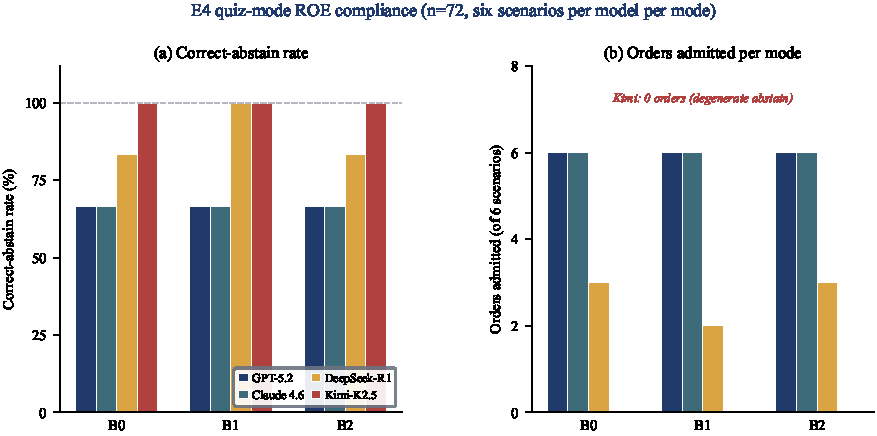
\includegraphics[width=\textwidth]{figures/fig_e4_roe.pdf}
\caption{E4 quiz-mode ROE compliance ($n=72$, six scenarios per model per mode). Panel~(a): correct-abstain rate by model and enforcement mode. DeepSeek-R1 reaches a perfect $6/6$ under B1 (audit-only); GPT-5.2 and Claude plateau at $4/6$ across all modes; Kimi achieves $6/6$ trivially via zero-order abstain. Panel~(b): orders admitted per mode, showing Kimi's degenerate policy (0 orders across all modes) and DeepSeek-R1's selective ordering.}
\label{fig:e4_roe}
\end{figure}

Three observations refine the abstract claim that LLM commanders are or are not ``ROE compliant.'' First, every model achieves $100\%$ verifier compliance on every order it issues across all three enforcement modes: the formal ROE check, when invoked, is rarely violated by orders that the model is willing to commit to. The B2 re-prompt mechanism therefore consumes \emph{zero} re-prompts in the quiz panel for all four models, so the K-budget convergence theorem (Theorem~\ref{thm:b2_kbudget}) is not exercised on this curated scenario set. Second, the model-level differential lies entirely in the \emph{correct-abstain} dimension: GPT-5.2 and Claude both decline to issue orders on $4$ of $6$ scenarios under every mode, while DeepSeek-R1 declines on $5$ of $6$ under B0 / B2 and on \emph{all six} under B1 (audit-only); the audit signal alone is sufficient to push DeepSeek-R1 from $5/6$ to $6/6$. Third, Kimi-K2.5 abstains on all six scenarios under every mode and admits no orders at all: this is vacuously perfect on the correct-abstain metric but is also a degenerate policy. The combined signal is that pre-registered hypothesis $H_{\mathrm{GATE}}$ (B2 strictly improves correct-abstain over B0) is \emph{not} confirmed on this six-scenario set: B1 achieves the largest improvement on DeepSeek-R1, and B2 leaves GPT-5.2 and Claude unchanged from B0. The six-scenario quiz set is statistically underpowered to falsify $H_{\mathrm{GATE}}$ at $n=6$ (Wilson 95\% CI half-width $\pm 35$~pp), so the live-mode CURC evaluation with hundreds of macro-tick decisions per game remains the discriminating test.

\paragraph{Experiment~E5: Cross-environment transfer.}\label{subsec:cross-env-transfer}
The five-domain panel (biology, legal, materials, RTS-engagement, Lux AI S3) plus the dynamic \texttt{sc2live} bridge enables a sixth experimental condition designed to test the central claim that DeFAb measures structural defeasible reasoning rather than vocabulary-bound knowledge retrieval. The script \texttt{experiments/cross\_env\_transfer.py} maintains a registry of six environments (\texttt{sc2live}, \texttt{rts\_engagement}, \texttt{lux\_ai\_s3}, \texttt{biology}, \texttt{legal}, \texttt{materials}) and evaluates a model under one configuration across all six in a single run, producing a row-per-environment Level~2 / Level~3 / graded-score table. The H5 hypothesis is that models fine-tuned on one domain (e.g., \texttt{sc2live} via the GRPO loop of Section~\ref{subsec:rlvr}) score comparably on Level~3 instances drawn from the other five environments, which would constitute positive evidence that the fine-tuning pipeline imparts a domain-general defeasible-reasoning capability rather than environment-specific pattern matching. The H5 evaluation is structurally orthogonal to the per-environment evaluations: it varies the \emph{environment} axis with the \emph{model} held fixed, while the prior evaluations vary the model with the environment held fixed. The script supports any \texttt{ModelInterface} provider (foundry, CURC vLLM, mock) and accepts a \texttt{--model} argument that points to a fine-tuned checkpoint, enabling direct comparison between base-model and post-DPO/post-GRPO transfer profiles.

\textbf{E5 base-model pilot.}
A 10-instance-per-environment pilot has been executed against GPT-5.2-chat and Claude Sonnet~4.6 (May~11, 2026; M4 direct, Foundry API). At Level~2 both models achieve $100\%$ on biology, legal, and materials (10/10 each); at Level~3 on the \texttt{rts\_engagement} ROE seed conflicts ($n=6$), GPT-5.2 achieves $66.7\%$ accuracy with mean graded score $0.67$ and Claude Sonnet~4.6 achieves $83.3\%$ with mean graded score $0.83$. The \texttt{sc2live} and \texttt{lux\_ai\_s3} rows of the table are blank in this pilot because their instance files are populated dynamically from live SC2 sessions and the queued Lux AI generation; they will be filled in once the corresponding traces complete on CURC. The Level~2 saturation across the three knowledge-base domains and the Level~3 spread between GPT and Claude on \texttt{rts\_engagement} establish a reproducible baseline against which fine-tuned checkpoints from Section~\ref{sec:finetuning} can be compared.


\subsection{Theoretical Properties}\label{subsec:sc2live-theory}

We close the SC2 section with three theoretical properties of the bridge. The ObservationLifter soundness theorem (Theorem~\ref{thm:lifter_sound}) was established in Section~\ref{subsec:sc2live-lifter}. The B2 K-budget convergence theorem (Theorem~\ref{thm:b2_kbudget}) was established in Section~\ref{subsec:sc2live-commander}. The remaining property is a conservativity-preservation bound under bounded observation noise.

\begin{theorem}[Conservativity preservation under bounded observation noise]\label{thm:conserv_noise}
Let $\D$ be the per-tick defeasible theory produced by lifting the true game state $\sigma$, and let $\widetilde\D$ be the theory produced by lifting a noisy observation $\widetilde\sigma$ that differs from $\sigma$ on at most $\epsilon$ ground facts (a bounded-noise model). Let $d$ be a candidate defeater that is conservative on $\D$. Then $d$ is conservative on $\widetilde\D$ except on at most $O(\epsilon \cdot |\Rd|)$ derived literals, where $|\Rd|$ is the number of defeasible rules in $\D$.
\end{theorem}

\begin{proof}[Proof sketch]
Conservativity of $d$ on $\D$ means that adding $d$ to $\D$ blocks the anomalous derivation but preserves every other defeasible derivation in $\D$. When the fact set is perturbed by at most $\epsilon$ facts, each perturbed fact can support or block at most $|\Rd|$ defeasible-rule firings (by structural induction over the dependency graph of $\Rd$). The total number of derived literals whose status changes between $\D$ and $\widetilde\D$ is therefore $O(\epsilon \cdot |\Rd|)$. Conservativity on $\widetilde\D$ reduces to conservativity on $\D$ except on this bounded set.
\end{proof}

The conservativity bound has direct deployment implications for the partial-observability mitigations of Section~\ref{subsec:sc2live-limits}: a per-tick observation noise of $\epsilon = 5$ facts on a KB with $|\Rd| = 32$ defeasible rules induces conservativity drift on at most $160$ derived literals per tick, of which only the literals on the conservativity check's specific anomaly set are visible to the verifier. In practice the per-tick conservativity drift is dominated by the $\epsilon = 0$ case (full observability after detection sweeps) and the bound is tighter than the worst-case product.


\section{Conclusion}\label{sec:conclusion}

We have introduced \textsc{DeFAb}, a benchmark for evaluating foundation models on defeasible abduction, and produced a layered empirical picture of current model capabilities. At Level~2 (rule abduction), all four frontier models achieve strong grounding accuracy ($72$--$79\%$ direct, formal modalities), confirming that the grounding deficit has been largely addressed by current training at this knowledge base scale.

At Level~3 (defeater abduction), the picture is more structured than a simple failure. Reasoning-optimized models (DeepSeek-R1 65\%, GPT-5.2 48\%) demonstrate substantial belief revision capability under a generation-appropriate chain-of-thought scaffold, while instruction-optimized models (Claude 16\%, Kimi 14\%) perform better under direct prompting. The CoT-sensitivity of reasoning-model performance---a 56--79 percentage-point swing from direct to CoT prompting---establishes that belief revision capability is \emph{latent} in these models rather than absent, but requires explicit prompting structure to surface reliably. The architectural dissociation (CoT helps reasoning models, hurts instruction models) is statistically confirmed and constitutes a distinct finding about how model families respond to different task formulations.

Two methodological findings have implications beyond this benchmark. First, the prompt-format confound at Level~3: a uniform CoT template (candidate-selection style) systematically underestimates reasoning-model capability on generation tasks. Evaluation designs for formal abductive benchmarks must separate selection-task and generation-task prompting protocols. Second, the narrative-modality bottleneck: all four models score 14--22\% on narrative rendering (M1) versus 73--94\% on formal modalities, a gap larger than any inter-model or inter-level difference---establishing that rendering robustness is a distinct evaluation dimension from logical reasoning capability.

DeFAb provides the formal infrastructure---polynomial-time instance generation, verifier-backed gold hypotheses, Wilson-CI-equipped rendering-robust accuracy, a McNemar-tested model comparison protocol, and synthetic contamination controls that isolate formal reasoning from memorized domain knowledge---to track progress on belief revision as training paradigms evolve. The preference optimization pipeline of Section~\ref{sec:finetuning} extends the benchmark from a passive evaluation instrument to an active training signal, exploiting the polynomial-time verifier as an exact reward function for DPO and RLHF. The defeasible conflict game framework (Section~\ref{subsec:conflict_games}) unifies preference optimization with adversarial self-play: game outcomes become structurally grounded preference pairs, the theory construction MDP (Section~\ref{subsec:theory_mdp}) provides a sequential environment for RLVR, the Active Inference formulation separates epistemic exploration from pragmatic revision mirroring the Lakatosian dialectic, and neural-guided tree search (Section~\ref{subsec:neural_search}) introduces AlphaZero-style expert iteration with learned policy and value networks over the derivation space---an approach validated at scale by AlphaProof for formal mathematics. The adversarial debate protocol of Section~\ref{sec:debate} adds a further dimension: competitive MCTS-driven agents that generate challenging evaluation instances adaptively and force models to defend derivations under proof perturbation. The \textsc{DeFAb-ROE} extension applies the same framework to rules of engagement using StarCraft~II as an unclassified proxy environment, producing a fourth domain (alongside biology, legal, and materials) in which the polynomial-time verifier scores ROE exception reasoning and the conservativity requirement enforces proportionality. The live \texttt{sc2live} bridge (Section~\ref{sec:sc2live}) extends this further: \texttt{ObservationLifter}, \texttt{ActionCompiler}, and \texttt{ReplayTraceExtractor} convert real game state and replays into defeasible theories on the same schema as \texttt{rts\_engagement}, while the Lux AI S3 KB provides a parallel game-grounded testbed at disjoint vocabulary, jointly enabling the cross-environment transfer experiment (Section~\ref{subsec:cross-env-transfer}) that directly probes whether DeFAb measures domain-general defeasible reasoning. The verifier-gated commander policy (B0/B1/B2 enforcement modes, Section~\ref{subsec:roe-compliance}) and the April-13 RTS-engagement Level~3 evaluation (Table~\ref{tab:rts_eval}) replicate the architectural dissociation reported on Tier~0 in a fully disjoint vocabulary domain, providing initial cross-domain support for the central thesis. The central open question is whether fine-tuning and debate---separately or in combination---can close the residual gap for instruction-tuned models (Claude, Kimi) for whom neither direct nor CoT prompting achieves high Level~3 accuracy. In Christie's terms: we have shown that some of today's detectives can, under the right conditions, override their deepest assumptions. The work that remains is understanding whether that override can be made robust, transferable, and independent of the prompting scaffold---and whether pitting detectives against one another sharpens the deductions of both. The M5 visual grounding modality opens a further dimension: whether the defeasible reasoning capabilities measured here transfer to multimodal settings where entity identification requires perception, connecting the formal revision framework to the emerging landscape of vision-language evaluation.


%%%%%%%%%%%%%%%%%%%%%%%%%%%%%%%%%%%%%%%%%%%%%%%%%%%%%%%%%%%%


%% =================================================================
%%  APPENDICES
%% =================================================================

\appendix

\section{Formal Definitions}\label{app:definitions}

\subsection{Signatures and Logic Programs}

\begin{definition}[Signature]\label{def:signature}
A first-order signature is a triple $\Sigma = (\mathcal{C}, \mathcal{F}, \mathcal{P})$ consisting of:
\begin{enumerate}[label=(\roman*)]
    \item a finite set of constants $\mathcal{C}$,
    \item a finite set of function symbols $\mathcal{F}$, each equipped with an arity $\mathrm{ar}(f) \geq 1$, and
    \item a finite set of predicate symbols $\mathcal{P}$, each equipped with an arity $\mathrm{ar}(p) \geq 0$.
\end{enumerate}
The Herbrand universe $\HU(\Sigma)$ is the set of all ground terms constructible from $\mathcal{C}$ and $\mathcal{F}$:
\[
    \HU(\Sigma) = \mathcal{C} \cup \{f(t_1, \ldots, t_{\mathrm{ar}(f)}) \mid f \in \mathcal{F},\; t_1, \ldots, t_{\mathrm{ar}(f)} \in \HU(\Sigma)\}.
\]
The Herbrand base $\HB(\Sigma)$ is the set of all ground atoms:
\[
    \HB(\Sigma) = \{p(t_1, \ldots, t_{\mathrm{ar}(p)}) \mid p \in \mathcal{P},\; t_1, \ldots, t_{\mathrm{ar}(p)} \in \HU(\Sigma)\}.
\]
When $\mathcal{F} = \emptyset$, we say $\Sigma$ is function-free (the datalog case), and $\HU(\Sigma) = \mathcal{C}$ is finite.
\end{definition}

\begin{definition}[Definite Logic Program]\label{def:deflp}
A definite logic program over $\Sigma$ is a finite set $\Pi$ of definite clauses of the form
\[
    h \leftarrow b_1, b_2, \ldots, b_n \qquad (n \geq 0)
\]
where $h, b_1, \ldots, b_n$ are atoms over $\Sigma$ (possibly containing variables from a countably infinite set $\mathcal{V}$). When $n = 0$, the clause is a fact. When $n > 0$, it is a rule with head $\head(c) = h$ and body $\mathrm{body}(c) = \{b_1, \ldots, b_n\}$. The ground instantiation is
\[
    \mathrm{ground}(\Pi) = \{h\theta \leftarrow b_1\theta, \ldots, b_n\theta \mid (h \leftarrow b_1, \ldots, b_n) \in \Pi,\; \theta: \mathcal{V} \to \HU(\Sigma)\}.
\]
\end{definition}

\begin{definition}[Immediate Consequence Operator]\label{def:tp}
The immediate consequence operator $T_\Pi : 2^{\HB} \to 2^{\HB}$ is
\[
    T_\Pi(I) = \bigl\{h\theta \mid (h \leftarrow b_1, \ldots, b_n) \in \Pi,\; \theta: \mathcal{V} \to \HU(\Sigma),\; \{b_1\theta, \ldots, b_n\theta\} \subseteq I\bigr\}.
\]
\end{definition}

\begin{definition}[Least Herbrand Model]\label{def:lhm}
The least Herbrand model of $\Pi$ is
\[
    \mathcal{M}_\Pi = \mathrm{lfp}(T_\Pi) = \bigcup_{i=0}^{\infty} T_\Pi^i(\emptyset).
\]
Existence and uniqueness follow from the Knaster--Tarski theorem, since $T_\Pi$ is monotone on $(2^{\HB}, \subseteq)$.
\end{definition}

\begin{definition}[SLD-Derivability]\label{def:sld}
A ground atom $q$ is SLD-derivable from $\Pi$, written $\Pi \pSLD q$, if there exists an SLD-refutation of $\leftarrow q$ from $\Pi$. For definite programs, $\Pi \pSLD q \iff q \in \mathcal{M}_\Pi$.
\end{definition}


\subsection{Defeasible Theories}

\begin{definition}[Defeasible Theory]\label{def:deftheory}
A defeasible theory is a quintuple $\D = (F, \Rs, \Rd, \Rdf, {\succ})$ where:
\begin{enumerate}[label=(\roman*)]
    \item $F \subseteq \HB$ is a finite set of facts;
    \item $\Rs$ is a finite set of strict rules: $r_s\colon b_1, \ldots, b_n \strictto h$;
    \item $\Rd$ is a finite set of defeasible rules: $r_d\colon b_1, \ldots, b_n \defto h$;
    \item $\Rdf$ is a finite set of defeaters: $r_{df}\colon b_1, \ldots, b_n \defeatto \neg h$; and
    \item ${\succ} \;\subseteq (\Rd \cup \Rdf) \times (\Rd \cup \Rdf)$ is an acyclic superiority relation.
\end{enumerate}
Write $A(r)$ for the antecedent of rule $r$, $C(r)$ for its consequent, $R = \Rs \cup \Rd \cup \Rdf$, and $|\D| = |F| + |R|$.
\end{definition}

\begin{definition}[Defeasible Derivation]\label{def:defderiv}
Let $\D$ be a propositional defeasible theory. A proof in $\D$ is a finite sequence of tagged literals $+\Delta q$, $-\Delta q$, $+\partial q$, or $-\partial q$.

$+\Delta q$ (definite provability) holds iff: (1) $q \in F$; or (2) $\exists\, r \in \Rs$ with $C(r) = q$ and $\forall\, a \in A(r)$: $+\Delta a$ holds.

$+\partial q$ (defeasible provability) holds iff: (1) $+\Delta q$; or (2) all of:
\begin{enumerate}[label=(\alph*)]
    \item $-\Delta \comp{q}$ (the complement is not definitely provable);
    \item $\exists\, r \in \Rd$ with $C(r) = q$ and $\forall\, a \in A(r)$: $+\partial a$ (an applicable rule for $q$ exists); and
    \item $\forall\, s \in \Rd \cup \Rdf$ with $C(s) = \comp{q}$: either
        (i) $\exists\, a \in A(s)$: $-\partial a$; or
        (ii) $\exists\, t \in \Rd$ with $C(t) = q$, $\forall\, a \in A(t)$: $+\partial a$, and $t \succ s$.
\end{enumerate}
We write $\D \pDelta q$ and $\D \pPartial q$ accordingly. The notation $\comp{q}$ denotes the complement: if $q = p$ then $\comp{q} = \neg p$; if $q = \neg p$ then $\comp{q} = p$.
\end{definition}

Condition (2c) embodies team defeat: every possible attack on $q$ must be individually neutralized.

\subsection{Conversion}

\begin{definition}[Partition Function]\label{def:partition}
A partition function for $\Pi$ is a mapping $\partfunc: \Pi \to \{s, d\}$.
\end{definition}

\begin{definition}[Defeasible Conversion]\label{def:conversion}
Given $\Pi$ and $\partfunc$, the defeasible conversion $\phi_\partfunc(\Pi) = (F_\partfunc, \Rs^{\partfunc}, \Rd^{\partfunc}, \emptyset, \emptyset)$ where:
\begin{align*}
    F_\partfunc &= \{h \mid (h \leftarrow) \in \Pi,\; \partfunc(h \leftarrow) = s\}, \\
    \Rs^{\partfunc} &= \{b_1, \ldots, b_n \strictto h \mid (h \leftarrow b_1, \ldots, b_n) \in \Pi,\; n > 0,\; \partfunc(\cdot) = s\}, \\
    \Rd^{\partfunc} &= \{b_1, \ldots, b_n \defto h \mid (h \leftarrow b_1, \ldots, b_n) \in \Pi,\; \partfunc(\cdot) = d\}
    \cup \{\top \defto h \mid (h \leftarrow) \in \Pi,\; \partfunc(h \leftarrow) = d\}.
\end{align*}
\end{definition}

\begin{definition}[Dependency Graph]\label{def:depgraph}
The dependency graph $G_\Pi = (V, E)$ has $V = \mathcal{P}$ and $(p, q) \in E$ iff some clause in $\Pi$ has head predicate $q$ and body predicate $p$. The depth of $p$ is the longest path from any source to $p$; predicates in cycles have depth $\infty$.
\end{definition}

\begin{definition}[Structured Partition Classes]\label{def:structpart}
We define four families:
\begin{enumerate}[label=(\roman*),nosep]
    \item $\partfunc_{\mathrm{leaf}}$: facts defeasible, rules strict.
    \item $\partfunc_{\mathrm{rule}}$: rules defeasible, facts strict.
    \item $\partfunc_{\mathrm{depth}}(k)$: clauses with head predicate depth $\leq k$ strict; deeper clauses defeasible.
    \item $\partfunc_{\mathrm{rand}}(\delta)$: each clause independently $d$ with probability $\delta$.
\end{enumerate}
\end{definition}

\begin{definition}[Partition Space]\label{def:partspace}
$\mathcal{K}(\Pi) = \{s, d\}^{|\Pi|}$. The defeasibility ratio is $\delta(\partfunc) = |\{c \in \Pi \mid \partfunc(c) = d\}|/|\Pi|$.
\end{definition}


\subsection{Support, Criticality, and Instance Generation}

\begin{definition}[Support Set]\label{def:support}
Given $\D$ and $q$ with $\D \pPartial q$, a support set is a minimal $S \subseteq F \cup \Rs \cup \Rd$ such that $(S \cap F, S \cap \Rs, S \cap \Rd, \emptyset, \succ|_S) \pPartial q$. Write $\Supp(\D, q)$ for the collection of all support sets.
\end{definition}

\begin{definition}[Full-Theory Criticality]\label{def:fullcrit}
$\CritStar(\D, q) = \{e \in F \cup \Rs \cup \Rd \mid \D \setminus \{e\} \not\pPartial q\}$. We have $\CritStar(\D, q) \subseteq \Crit(\D, q)$ (Proposition~\ref{prop:critinclusion}).
\end{definition}

\begin{definition}[Redundancy Degree]\label{def:redundancy}
$\mathrm{red}(e, \D, q) = |\{S \in \Supp(\D, q) \mid e \notin S\}|$. If $\mathrm{red}(e, \D, q) = 0$, then $e \in \CritStar(\D, q)$.
\end{definition}

\begin{definition}[Abductive Instance]\label{def:instance}
Given $\D$, target $q$, and $e \in \CritStar(\D, q)$: (1) form $\Dm = \D \setminus \{e\}$; (2) sample $k$ syntactically similar distractors; (3) compute $\Hgold = \{h \mid \Dm \cup \{h\} \pPartial q,\; h \text{ minimal}\}$.
\end{definition}

\begin{definition}[Complexity Stratification]\label{def:levels12}
Level 1: $e \in F$ (fact completion). Level 2: $e \in \Rd$ (rule abduction). Level 3: defeater abduction (Section~\ref{subsec:level3detail}).
\end{definition}

\begin{definition}[Defeasible Yield]\label{def:yield}
$Y(\partfunc, Q) = \sum_{q \in Q} |\CritStar(\D_\partfunc, q)|$ for target set $Q \subseteq \mathcal{M}_\Pi$.
\end{definition}


\subsection{Level 3: Anomalies and Defeater Abduction}\label{subsec:level3detail}

\begin{definition}[Expectation Set]\label{def:expectation}
$\Exp(\D) = \{q \mid \D \pPartial q\}$.
\end{definition}

\begin{definition}[Anomaly]\label{def:anomclass}
A ground literal $\alpha$ is an anomaly if $\D \pPartial \comp{\alpha}$. It is strict if $\D \pDelta \comp{\alpha}$ (excluded from Level 3), and defeasible if $\D \pPartial \comp{\alpha}$ and $\D \not\pDelta \comp{\alpha}$.
\end{definition}

\begin{definition}[Anomaly Support]\label{def:ansup}
The derivation tree $\mathcal{T}(\D, q)$ is the AND-OR tree of the proof of $+\partial q$. The anomaly support is $\AnSup(\D, \alpha) = \{r \in \Rd \mid r \text{ appears in } \mathcal{T}(\D, \comp{\alpha})\}$.
\end{definition}

\begin{definition}[Language Bias]\label{def:langbias}
$\La = (\mathcal{P}^+, \mathcal{P}^-, \mathrm{ar}_{\max}, d_{\max})$ specifies permitted antecedent predicates $\mathcal{P}^+$, consequent predicates $\mathcal{P}^-$, maximum antecedent length $\mathrm{ar}_{\max}$, and maximum nesting depth $d_{\max}$.
\end{definition}

\begin{definition}[Candidate Spaces]\label{def:candspace}
The candidate defeater space is
\[
    \Rdfspace(\La) = \left\{r\colon b_1, \ldots, b_m \defeatto \neg h \;\middle|\;
    m \leq \mathrm{ar}_{\max},\;
    \pred(b_i) \in \mathcal{P}^+,\;
    \pred(h) \in \mathcal{P}^-,\;
    \mathrm{vars}(h) \subseteq \textstyle\bigcup_i \mathrm{vars}(b_i)
    \right\}
\]
and the candidate exception space $\Rdexcspace(\La)$ is defined identically with $\defto$ replacing $\defeatto$.
\end{definition}

\begin{definition}[Defeater Abduction Problem]\label{def:dap}
Given $\D$, a defeasible anomaly $\alpha$, and $\La$: find $r \in \Rdfspace(\La) \cup \Rdexcspace(\La)$, possibly with superiority assertions $\Gamma$, such that $\D \cup \{r\} \cup \Gamma \cup \{\alpha\} \not\pPartial \comp{\alpha}$.
\end{definition}

\begin{definition}[Resolution Strength]\label{def:resstrength}
Let $\D' = \D \cup \{r\} \cup \Gamma \cup \{\alpha\}$.
\begin{enumerate}[label=(\roman*),nosep]
    \item Weak: $\D' \not\pPartial \comp{\alpha}$ and $\D' \not\pPartial \alpha$.
    \item Strong: $r \in \Rdexcspace(\La)$, $\Gamma \neq \emptyset$, and $\D' \pPartial \alpha$.
    \item Restructuring: $\D'$ derives $\alpha$ and preserves all $q \in \Exp(\D) \setminus \{\comp{\alpha}\}$.
\end{enumerate}
\end{definition}

\begin{remark}[AGM Correspondence]\label{rem:agm}
Conservativity specializes the AGM recovery postulate \cite{alchourron1985logic} to the defeasible setting. In AGM terms, if a belief set $K$ is revised by new evidence $\alpha$ to obtain $K^*_\alpha$, recovery requires $(K \cap K^*_\alpha) + \alpha = K^*_\alpha$: nothing is lost beyond what accommodation of $\alpha$ strictly requires. Our conservativity check verifies this for the defeasible expectation set: $\Exp(\D \cup \Delta \cup \{\alpha\}) \supseteq \Exp(\D) \setminus \{\comp{\alpha}\}$. The key difference is that defeasible theories make the check \emph{tractable}: each expectation can be verified in polynomial time (Theorem~\ref{thm:derivP}), whereas AGM revision over arbitrary belief sets is in general undecidable.
\end{remark}

\begin{definition}[Level 3 Instance Generation]\label{def:level3gen}
Given complete theory $\Dfull$ with $\Rdf \neq \emptyset$ or ${\succ} \neq \emptyset$: (1) select $r^*$; (2) find $\alpha$ with $\Dfull \pPartial \alpha$ and $\Dfull \setminus \{r^*\} \pPartial \comp{\alpha}$; (3) form $\Dm$ by removing $r^*$ and all superiority assertions involving it; (4) verify $\Dm \pPartial \comp{\alpha}$ and $\Dm \not\pDelta \comp{\alpha}$; (5) compute $\Rgold$.
\end{definition}


\subsection{Novelty and Difficulty}

\begin{definition}[Predicate Novelty]\label{def:novelty}
$\Nov(r, \Dm) = |\pred(r) \setminus \pred(\Dm)| / |\pred(r)|$, where $\pred(\cdot)$ extracts predicate symbols.
\end{definition}

\begin{remark}[Relation to Dalal Distance]\label{rem:dalal}
Revision distance is a defeasible analogue of Dalal's \cite{dalal1988investigations} Hamming-distance approach to belief revision, which measures revision cost as the number of propositional variables whose truth value changes between the nearest models of the original and revised theories. Our formulation substitutes \emph{structural changes} (rules and facts added, $|\Delta|$) and \emph{expectation changes} (conclusions lost) for Dalal's model-level bit flips, yielding a distance that is both interpretable and polynomial-time computable. A conservative resolution achieves $d_{\mathrm{rev}} = |\Delta|$ (the expectation-loss term vanishes), the minimum possible cost for a revision that adds $|\Delta|$ new elements.
\end{remark}

\begin{definition}[Structural Difficulty]\label{def:structdiff}
$\sigma(I) = (\ell(I),\; |\Supp(\D, q)|,\; |\Hgold|,\; \min_{h \in \Hgold} |h|,\; \Nov^*(I))$, where $\Nov^*(I) = \min_{h \in \Hgold} \Nov(h, \Dm)$.
\end{definition}


\subsection{Synthetic Theory Generation}\label{subsec:synthetic_defs}

\begin{definition}[Synthetic Vocabulary]\label{def:synthvocab}
A synthetic vocabulary $\mathcal{V}_{\mathrm{syn}} = (\mathcal{P}_{\mathrm{syn}}, \mathcal{C}_{\mathrm{syn}})$ is a pair of finite sets of predicate names and constant names generated by a context-free grammar $G_{\mathrm{syl}}$ over phonotactically valid syllable templates. The grammar produces strings of 2--4 syllables from templates $\{$CV, CVC, CVCV, CVCCV$\}$ where C is drawn from English consonant inventory and V from English vowel inventory. Each generated string is verified for zero occurrence in a reference web corpus $\mathcal{W}$ (Common Crawl via the \texttt{infini-gram} index): $\forall\, w \in \mathcal{V}_{\mathrm{syn}}$: $\mathrm{count}(w, \mathcal{W}) = 0$.
\end{definition}

\begin{definition}[Synthetic Theory Generation]\label{def:synthgen}
The generation procedure $\mathrm{Gen}(\Theta, \mathcal{V}_{\mathrm{syn}})$ with structural parameters $\Theta = (n_F, n_{\Rs}, n_{\Rd}, n_{\Rdf}, d, b, a)$ produces a synthetic defeasible theory $\D_{\mathrm{syn}}$ as follows:
\begin{enumerate}[label=(\roman*),nosep]
    \item \textbf{Graph generation.} Sample a directed acyclic graph $G = (V, E)$ with $|V| = |\mathcal{P}_{\mathrm{syn}}|$ nodes, maximum depth $d$, and average branching factor $b$, by iterative layer construction: layer $0$ contains $\lceil |V|/d \rceil$ source nodes; each subsequent layer $i$ connects each node to $b \pm 1$ parent nodes in layer $i-1$ (uniformly sampled).
    \item \textbf{Fact generation.} For each source predicate $p \in V$ with $\mathrm{depth}(p) = 0$, generate $\lfloor n_F / |V_0| \rfloor$ ground facts by instantiating $p$ with constants drawn uniformly from $\mathcal{C}_{\mathrm{syn}}$, up to arity $a$.
    \item \textbf{Rule generation.} For each edge $(p_1, \ldots, p_m, q) \in E$ (where $p_1, \ldots, p_m$ are predecessors of $q$ in $G$), generate a rule with antecedent predicates $\{p_1, \ldots, p_m\}$ and consequent $q$. Rules at depth $\leq k$ are assigned to $\Rs^{\mathrm{syn}}$ (strict); deeper rules are assigned to $\Rd^{\mathrm{syn}}$ (defeasible), mirroring $\partfunc_{\mathrm{depth}}(k)$.
    \item \textbf{Defeater generation.} For each target defeasible rule $r_d \in \Rd^{\mathrm{syn}}$ designated for Level~3 instance generation, construct a defeater $r^* \in \Rdf^{\mathrm{syn}}$ with antecedent drawn from $\mathcal{P}_{\mathrm{syn}}$ and consequent $\comp{C(r_d)}$, together with $r^* \succ r_d$. Verify conservativity of $r^*$ by the procedure of Definition~\ref{def:level3gen}.
    \item \textbf{Verification.} Confirm that $\D_{\mathrm{syn}} \pPartial q$ for all designated targets $q$, that all defeaters resolve their intended anomalies conservatively, and that the structural difficulty tuple $\sigma(I_{\mathrm{syn}})$ lies within the target distribution.
\end{enumerate}
\end{definition}

\begin{definition}[Structural Matching]\label{def:structmatch}
Given a naturalistic instance $I_{\mathrm{nat}}$ and a pool of synthetic instances $\{I_{\mathrm{syn}}^{(j)}\}$, the structural match is $I_{\mathrm{syn}}^* = \arg\min_j \| \hat\sigma(I_{\mathrm{nat}}) - \hat\sigma(I_{\mathrm{syn}}^{(j)}) \|_1$, where $\hat\sigma$ is the component-wise normalization of $\sigma$ to $[0,1]$ by the range of each component over the full instance set, extended to include theory size $|\D|$, defeasibility ratio $\delta(\partfunc)$, and (for Level~3) the novelty $\Nov^*$ and revision distance $d_{\mathrm{rev}}^*$ of gold-standard resolutions.
\end{definition}

\begin{proposition}[Synthetic Instance Validity]\label{prop:synthvalid}
For any $\Theta$ satisfying $n_F \geq 1$, $d \geq 1$, $b \geq 1$, $a \geq 1$, and $n_{\Rs} + n_{\Rd} \geq 1$, the procedure $\mathrm{Gen}(\Theta, \mathcal{V}_{\mathrm{syn}})$ terminates and produces a valid defeasible theory $\D_{\mathrm{syn}}$ satisfying all properties of Definition~\ref{def:deftheory}. All instances generated from $\D_{\mathrm{syn}}$ via the pipeline of Sections~\ref{subsec:abduction}--\ref{subsec:level3} satisfy the same validity guarantees as naturalistic instances.
\end{proposition}

\begin{proof}
Termination follows from the finiteness of $\mathcal{V}_{\mathrm{syn}}$ and the DAG structure of $G$. Validity of $\D_{\mathrm{syn}}$ as a defeasible theory follows by construction: facts are ground atoms, rules have the required form, and $\succ$ is acyclic (inherited from the DAG). The instance generation pipeline is agnostic to the semantic content of predicate and constant names, depending only on the formal structure $\D_{\mathrm{syn}}$; all pipeline guarantees (Propositions~\ref{prop:goldnonempty}--\ref{prop:goldnonuniq}, Corollary~\ref{cor:cubic}) therefore transfer.
\end{proof}


\subsection{Rendering}\label{subsec:rendering_defs}

\begin{definition}[Rendering Codec]\label{def:codec}
A rendering codec $\rho = (\rho_{\mathrm{enc}}, \rho_{\mathrm{dec}})$ maps a theory with target and candidates to a token sequence (prompt), and maps a token sequence (response) to candidate rules or $\bot$.
\end{definition}

\begin{definition}[Faithfulness]\label{def:faithful}
$\rho_{\mathrm{enc}}$ is faithful w.r.t.\ ideal reasoners $\mathfrak{R}$ if $R(\rho_{\mathrm{enc}}(\Dm, q, \Hcand)) \cap \Hgold \neq \emptyset$ for every $R \in \mathfrak{R}$ and instance with $\Hgold \neq \emptyset$.
\end{definition}

\begin{definition}[Naturalness]\label{def:naturalness}
$\Nat(\rho_{\mathrm{enc}}) = \mathbb{E}_{(\D, q) \sim \mathcal{P}}[\log p_{\mathcal{T}}(\rho_{\mathrm{enc}}(\Dm, q, \Hcand))]$, where $p_\mathcal{T}$ is the density of a reference language model.
\end{definition}

\begin{definition}[Rendering Modalities]\label{def:modalities}
Five encoding strategies. The first four trade naturalness against faithfulness:
(M1) narrative, (M2) semi-formal, (M3) annotated formal, (M4) pure formal. The fifth is cross-modal: (M5) visual grounding, which presents entity-grounding facts as images sourced from linked knowledge bases (Wikidata P18, VisualSem, BabelNet) while retaining M4 formal syntax for theory rules, target, and candidates. M5 has two sub-variants: M5-replace (images only, entity names hidden) and M5-supplement (images alongside textual entity names). See Appendix~\ref{app:rendering} for templates.
\end{definition}

\begin{definition}[Modality Ordering]\label{def:modorder}
$\Nat(\rho^{\mathrm{nar}}) \geq \Nat(\rho^{\mathrm{semi}}) \geq \Nat(\rho^{\mathrm{form}}) \geq \Nat(\rho^{\mathrm{pure}})$ and $\Faith(\rho^{\mathrm{pure}}) \geq \Faith(\rho^{\mathrm{form}}) \geq \Faith(\rho^{\mathrm{semi}}) \geq \Faith(\rho^{\mathrm{nar}})$.
\end{definition}

\begin{definition}[Ontological Grounding Map]\label{def:nlmap}
$\NL: \HB \to \La^*$ satisfying: (i) injectivity; (ii) compositionality via $\NL_\mathcal{P}$ and $\NL_\mathcal{C}$; (iii) domain coherence.
\end{definition}

\begin{definition}[Decoder Strategies]\label{def:decoder}
(D1) Exact match. (D2) Template extraction via $\arg\min_r d_{\mathrm{edit}}(y, \tau(r))$. (D3) Semantic extraction via parser $M_{\mathrm{parse}}(y \mid \mathrm{schema}(\La))$.
\end{definition}

\begin{definition}[Round-Trip Consistency]\label{def:roundtrip}
$\rho_{\mathrm{dec}}(\tau(r)) = r$ for every $r$ in the candidate space.
\end{definition}

\begin{definition}[Rendering-Robust Accuracy]\label{def:robustacc}
$\mathrm{Acc}_{\mathrm{robust}}(M) = \frac{1}{N} \sum_{i=1}^N \min_{j} \Pr_M[h \in \Hgold_i \mid \rho^{(j)}_{\mathrm{enc}}(I_i)]$, where $j$ ranges over the text modalities M1--M4. M5 accuracy is reported separately for vision-capable models.
\end{definition}

\begin{definition}[Empirical Difficulty]\label{def:empdiff}
$\Diff_\rho(I, M) = 1 - \Pr_M[\rho_{\mathrm{dec}}(M(\rho_{\mathrm{enc}}(\Dm, q))) \in \Hgold]$.
\end{definition}


%% =================================================================
\section{Proofs}\label{app:proofs}

\begin{proposition}[Conservativity of Strict Conversion]\label{prop:strict}
If $\partfunc \equiv s$, then $q \in \mathcal{M}_\Pi \iff \D_\partfunc \pDelta q$.
\end{proposition}

\begin{proof}
When $\partfunc \equiv s$, we have $\Rd^{\partfunc} = \emptyset$, and the strict fragment $(\Rs^{\partfunc}, F_\partfunc)$ is isomorphic to $\Pi$ via $(h \leftarrow b_1, \ldots, b_n) \mapsto (b_1, \ldots, b_n \strictto h)$ for rules and $(h \leftarrow) \mapsto h \in F$ for facts. The definite provability relation $\pDelta$ on the strict fragment coincides with iterated application of $T_\Pi$, so $\{q \mid \D_\partfunc \pDelta q\} = \mathrm{lfp}(T_\Pi) = \mathcal{M}_\Pi$.
\end{proof}

\begin{proposition}[Defeasible Preservation]\label{prop:defpres}
For any $\partfunc$, if $q \in \mathcal{M}_\Pi$ and $\D_\partfunc$ contains no rules with consequent $\comp{q}$, then $\D_\partfunc \pPartial q$.
\end{proposition}

\begin{proof}
Without rules having consequent $\comp{q}$, condition (2c) of Definition~\ref{def:defderiv} is vacuously satisfied. Condition (2b) is met by the rules deriving $q$ in $\Pi$, whether classified as strict or defeasible, since the same body literals remain provable by induction on derivation depth.
\end{proof}

\begin{proposition}[Monotonicity of Expected Yield]\label{prop:yieldmono}
$\mathbb{E}[Y(\partfunc_{\mathrm{rand}}(\delta), Q)]$ is non-decreasing in $\delta$.
\end{proposition}

\begin{proof}
Increasing $\delta$ converts strict rules to defeasible rules, expanding the set of ablation-eligible elements. For $\partfunc, \partfunc'$ differing only in $\partfunc(c) = s$ and $\partfunc'(c) = d$, we have $\CritStar(\D_{\partfunc'}, q) \supseteq \CritStar(\D_\partfunc, q)$.
\end{proof}

\begin{proposition}\label{prop:critinclusion}
$\CritStar(\D, q) \subseteq \Crit(\D, q)$, with possibly strict inclusion.
\end{proposition}

\begin{proof}
If $e \in \CritStar(\D, q)$, then $\D \setminus \{e\} \not\pPartial q$, so for any support set $S$ containing $e$, $S \setminus \{e\} \not\pPartial q$. Strict inclusion occurs when $e$ belongs to some minimal support set but alternative derivation paths bypass it.
\end{proof}

\begin{theorem}[Defeasible Derivation in P]\label{thm:derivP}
For propositional defeasible theories without defeaters and with acyclic $\succ$, deciding $\D \pPartial q$ is in P, computable in $O(|R| \cdot |F|)$ time \cite{maher2001propositional, billington2010framework}.
\end{theorem}

\begin{proof}
The tagged proof procedure implements as forward chaining over tagged literals, iterating until a fixed point. Each iteration processes each rule at most once; the iteration count is bounded by $|F| + |R|$. Checking applicability and team defeat per iteration costs $O(|R|)$. Total: $O(|R| \cdot (|F| + |R|))$.
\end{proof}

\begin{corollary}\label{cor:verif}
Verifying $\Dm \cup \{h\} \pPartial q$ is in P.
\end{corollary}

\begin{theorem}[Minimum Support Set is NP-Complete]\label{thm:suppNP}
Given $\D$, $q$ with $\D \pPartial q$, and integer $k$: deciding $\exists\, S \in \Supp(\D, q)$ with $|S| \leq k$ is NP-complete.
\end{theorem}

\begin{proof}
NP membership: guess $S$ with $|S| \leq k$, verify sufficiency (P by Theorem~\ref{thm:derivP}) and minimality ($|S|$ P-time checks).

NP-hardness: reduce from Minimum Hitting Set. Given universe $U = \{u_1, \ldots, u_m\}$ and collection $\mathcal{S} = \{S_1, \ldots, S_\ell\}$, construct:
\begin{itemize}[nosep]
    \item Defeasible rules $r_i\colon \top \defto u_i$ for each $u_i$.
    \item Strict rules $s_j\colon u_{j_1}, \ldots, u_{j_t} \strictto p_j$ for each $S_j = \{u_{j_1}, \ldots, u_{j_t}\}$.
    \item Final strict rule $s_{\mathrm{all}}\colon p_1, \ldots, p_\ell \strictto q$.
\end{itemize}
Support sets for $q$ restricted to defeasible rules correspond bijectively to hitting sets of $\mathcal{S}$.
\end{proof}

\begin{theorem}\label{thm:critP}
$\CritStar(\D, q)$ is computable in $O(|\D|^2 \cdot |F|)$ time.
\end{theorem}

\begin{proof}
Test $\D \setminus \{e\} \pPartial q$ for each of the $|\D|$ elements $e$; each test costs $O(|R| \cdot |F|)$.
\end{proof}

\begin{corollary}\label{cor:cubic}
The full instance generation pipeline runs in $O(|\D|^3)$.
\end{corollary}

\begin{theorem}[First-Order Complexity]\label{thm:firstorder}
Deciding $\D \pPartial q$ for first-order defeasible theories is EXPTIME-complete in general. For the function-free (datalog) fragment, the pipeline remains in P with respect to the grounded size.
\end{theorem}

\begin{proof}
The ground instantiation has size $O(|\D| \cdot |\mathcal{C}|^a)$ where $a = \max_p \mathrm{ar}(p)$. With function symbols, grounding can be exponential. Without function symbols, $|\HU| = |\mathcal{C}|$ and grounding is polynomial in $|\mathcal{C}|^a$.
\end{proof}

\begin{proposition}[Candidate Space Size]\label{prop:candsize}
For a function-free signature with $|\mathcal{P}^+| = p$, max arity $a$, $|\mathcal{C}| = c$:
$|\Rdfspace(\La)| = O(|\mathcal{P}^-| \cdot c^a \cdot \sum_{m=0}^{\mathrm{ar}_{\max}} \binom{p \cdot c^a}{m})$.
For fixed $\mathrm{ar}_{\max}$ this is polynomial in $|\Sigma|$.
\end{proposition}

\begin{theorem}[DAP Complexity]\label{thm:dapcomplex}
(i) Weak resolution with bounded $\mathrm{ar}_{\max}$: NP-complete. (ii) Strong resolution: $\Sigma_2^P$-complete. (iii) Conservative restructuring: $\Sigma_2^P$-hard.
\end{theorem}

\begin{proof}
(i) NP membership: guess $r \in \Rdfspace(\La)$ (polynomial), verify $\D \cup \{r, \alpha\} \not\pPartial \comp{\alpha}$ in P. Hardness: reduce from SAT. Given CNF $\phi = C_1 \wedge \cdots \wedge C_m$ over $x_1, \ldots, x_n$, construct:
\begin{itemize}[nosep]
    \item Facts $\mathrm{var}(x_i)$; defeasible rules $r_i^\pm\colon \mathrm{var}(x_i) \defto \mathrm{pos/neg}(x_i)$.
    \item Strict rules deriving $\mathrm{sat}(C_j)$ from appropriate literals; conjunction rule to $\mathrm{sat\_all}$.
    \item Default $r_\neg\colon \top \defto \neg\mathrm{sat\_all}$; anomaly $\alpha = \mathrm{sat\_all}$.
\end{itemize}
An applicable defeater encodes a satisfying assignment.

(ii) The existential guess of $r$ and $\Gamma$ is polynomial; verifying all attacks are neutralized is in coNP. Hardness via $\exists\forall$-QBF \cite{eiter1995complexity}.

(iii) Follows from (ii).
\end{proof}

\begin{proposition}[Gold Set Non-Emptiness]\label{prop:goldnonempty}
In Definition~\ref{def:level3gen}, $r^* \in \Rgold$ provided it satisfies $\La$.
\end{proposition}

\begin{proposition}[Gold Set Non-Uniqueness]\label{prop:goldnonuniq}
In general $|\Rgold| > 1$, with resolutions of different strengths.
\end{proposition}

\begin{proposition}\label{prop:difforder}
Expected empirical difficulty respects the level ordering: $\mathbb{E}[\Diff(\ell{=}1)] \leq \mathbb{E}[\Diff(\ell{=}2)] \leq \mathbb{E}[\Diff(\ell{=}3)]$.
\end{proposition}

\begin{proof}
Each level subsumes the reasoning of the previous and introduces additional requirements. The search space grows from $|F|$ (Level 1) through $|\Rd|$ (Level 2) to $|\Rdfspace(\La) \cup \Rdexcspace(\La)|$ (Level 3, Proposition~\ref{prop:candsize}), with the conservativity constraint further reducing the effective gold set relative to the search space.
\end{proof}


%% =================================================================
\section{Rendering Details}\label{app:rendering}

\subsection{Encoder Templates}

Narrative rendering (M1) uses:
\begin{align*}
    \tau_1(b_1, \ldots, b_n \strictto h) &= \text{``It is always the case that if } \NL(b_1) \text{ and \ldots\ and } \NL(b_n)\text{, then } \NL(h)\text{.''} \\
    \tau_1(b_1, \ldots, b_n \defto h) &= \text{``Typically, if } \NL(b_1) \text{ and \ldots\ and } \NL(b_n)\text{, then } \NL(h)\text{.''} \\
    \tau_1(b_1, \ldots, b_n \defeatto \neg h) &= \text{``The fact that } \NL(b_1) \text{ and \ldots\ may cast doubt on whether } \NL(h)\text{.''} \\
    \tau_1(r \succ s) &= \text{``The principle in [}\mathrm{label}(r)\text{] takes precedence over [}\mathrm{label}(s)\text{] when both apply.''}
\end{align*}

Semi-formal rendering (M2): $\tau_2(b_1, \ldots, b_n \defto h) = \text{``}\NL(b_1) \wedge \ldots \wedge \NL(b_n) \Rightarrow \NL(h)\ [\text{defeasible}]\text{''}$.

Annotated formal (M3): $\tau_3(r) = \mathrm{code}(r) \;\|\; \text{``\% ''} \circ \tau_1(r)$.

Pure formal (M4): raw logical syntax without glosses.

Visual grounding (M5) retains the M4 pure formal encoding for all theory rules, superiority relations, target queries, and candidate hypotheses. Entity-grounding facts are modified depending on the sub-variant:
\begin{itemize}[nosep]
\item M5-replace: \texttt{bird([IMAGE:TWEETY]).} --- the entity name is replaced by an image reference; the model receives only the image.
\item M5-supplement: \texttt{bird(tweety). \% [IMAGE:TWEETY]} --- the entity name is retained and annotated with a co-presented image.
\end{itemize}
Images are sourced from linked knowledge bases via Wikidata P18 properties, VisualSem synset mappings, and BabelNet image APIs. An \texttt{ImageManifest} indexes entity-to-image associations with source-priority selection (Wikidata $>$ VisualSem $>$ BabelNet). The coverage ratio $c(\D, \mathcal{I}) = |\{e \in \mathrm{entities}(\D) : \mathcal{I}(e) \neq \emptyset\}| / |\mathrm{entities}(\D)|$ measures the fraction of theory entities with available images; M5 instances require $c \geq \theta$ for a configurable threshold~$\theta$.

Narrative mode uses implicit universal quantification (``Proteins typically have stable three-dimensional structure''); formal modes use explicit quantification ($\forall X.\; \mathrm{protein}(X) \Rightarrow \mathrm{has\_stable\_3d}(X)$).

\subsection{Decoder Properties}

\begin{proposition}\label{prop:decprop}
\begin{center}
\begin{tabular}{@{}lccc@{}}
\toprule
Strategy & Sound & Complete & Faithful \\
\midrule
(D1) Exact match & \checkmark & $\times$ & \checkmark \\
(D2) Template extraction & \checkmark & \checkmark & conditional$^\dagger$ \\
(D3) Semantic extraction & conditional$^\ddagger$ & \checkmark & approximate \\
\bottomrule
\end{tabular}
\end{center}
$^\dagger$ Faithful iff $\tau$ is injective and the edit-distance minimum is unique.
$^\ddagger$ Sound iff $M_{\mathrm{parse}}$ outputs only well-formed rules.
\end{proposition}

\begin{proposition}[Round-Trip Conditions]\label{prop:roundtrip}
(i) $\rho_{\mathrm{dec}}^{\mathrm{exact}}$ satisfies round-trip consistency by construction. (ii) $\rho_{\mathrm{dec}}^{\mathrm{templ}}$ satisfies it iff $\tau$ is injective. (iii) $\rho_{\mathrm{dec}}^{\mathrm{sem}}$ satisfies it approximately, measurable via synthetic tests.
\end{proposition}

\subsection{Modality--Level Interaction}

\begin{conjecture}\label{conj:modlevel}
For Level 1 tasks, narrative rendering yields highest accuracy (cloze-like). For Level 3 tasks, semi-formal or formal rendering yields highest accuracy (logical structure must be precisely specified). For M5 (visual grounding) tasks, we conjecture that the perception--reasoning interaction produces accuracy below M4 (pure formal) but above M1 (narrative): the visual grounding challenge is harder than reading formal syntax but easier than parsing full natural language, since the logical structure of the theory remains in formal notation while only entity identification requires cross-modal inference. If confirmed, this places the visual perception bottleneck between the linguistic bottleneck (M1) and pure logical reasoning (M4) on the modality difficulty spectrum. More broadly, if confirmed, this implies different reasoning tasks require different communication modalities between formal systems and neural models.
\end{conjecture}


%% =================================================================
\section{Worked Example}\label{app:example}

\begin{figure}[h]
\centering
\resizebox{0.9\textwidth}{!}{% Figure 4: IDP defeater abduction worked example.
% Appendix-sized figure (text-width). 2x2 panel grid with absolute coords.
% No nested tikzpictures. Score boxes are inline \colorbox labels.
%
% Grid (anchor=north west on every panel):
%   Top-left  (i)   Complete theory D_full     at (0,    0)
%   Top-right (ii)  Challenge theory D-        at (8.0,  0)
%   Bot-left  (iii) Anomaly surfaces           at (0,   -5.5)
%   Bot-right (iv)  Graded resolutions         at (8.0, -5.5)
%
% Each panel: 7.0cm wide, 5.0cm tall, anchored top-left.
% Inter-panel horizontal gap: 1.0cm (8.0 - 7.0). Vertical gap: 0.5cm.
% Arrows are drawn last, between named anchors.
%
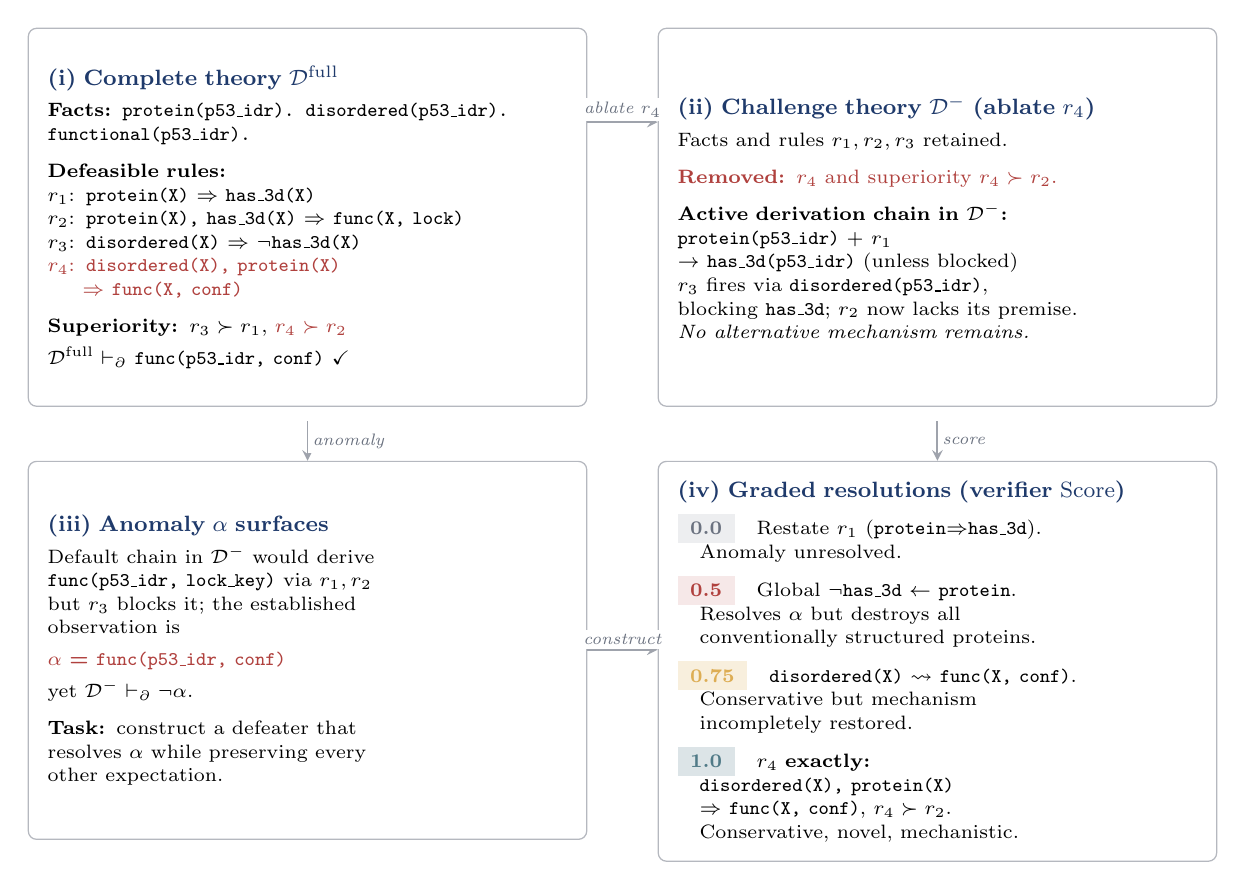
\begin{tikzpicture}[
    >=stealth,
    panel/.style={
        draw=defabGray!50, rounded corners=3pt,
        inner sep=7pt, align=left, fill=white,
        font=\fontsize{7}{8.5}\selectfont,
        line width=0.45pt,
        text width=6.6cm, minimum height=4.8cm, anchor=north west
    },
    % inter-panel arrows
    flow/.style={->, thick, color=defabGray!65, line width=0.7pt},
    flowlbl/.style={
        font=\fontsize{6.5}{7.5}\selectfont\itshape,
        text=defabGray, fill=white, inner sep=1.5pt
    },
]

%% =================================================================
%% Panel (i): Complete theory D_full   (top-left)
%% =================================================================
\node[panel] at (0, 0) (p1) {
  {\fontsize{8}{9.5}\selectfont\bfseries\color{defabBlue}(i) Complete theory $\Dfull$}\\[3pt]
  \textbf{Facts:} \texttt{protein(p53\_idr).} \texttt{disordered(p53\_idr).}\\
  \texttt{functional(p53\_idr).}\\[5pt]
  \textbf{Defeasible rules:}\\
  $r_1$: \texttt{protein(X) $\Rightarrow$ has\_3d(X)}\\
  $r_2$: \texttt{protein(X), has\_3d(X) $\Rightarrow$ func(X, lock)}\\
  $r_3$: \texttt{disordered(X) $\Rightarrow$ $\neg$has\_3d(X)}\\
  {\color{defabRed}$r_4$: \texttt{disordered(X), protein(X)}}\\
  \phantom{$r_4$:\ }{\color{defabRed}\texttt{$\Rightarrow$ func(X, conf)}}\\[5pt]
  \textbf{Superiority:} $r_3 \succ r_1$, {\color{defabRed}$r_4 \succ r_2$}\\[3pt]
  $\Dfull \pPartial$ \texttt{func(p53\_idr, conf)} \checkmark
};

%% =================================================================
%% Panel (ii): Challenge theory D-   (top-right)
%% =================================================================
\node[panel] at (8.0cm, 0) (p2) {
  {\fontsize{8}{9.5}\selectfont\bfseries\color{defabBlue}(ii) Challenge theory $\Dm$ (ablate $r_4$)}\\[3pt]
  Facts and rules $r_1, r_2, r_3$ retained.\\[5pt]
  {\color{defabRed}\textbf{Removed:} $r_4$ and superiority $r_4 \succ r_2$.}\\[5pt]
  \textbf{Active derivation chain in $\Dm$:}\\
  \texttt{protein(p53\_idr)} + $r_1$\\
  $\to$ \texttt{has\_3d(p53\_idr)} (unless blocked)\\
  $r_3$ fires via \texttt{disordered(p53\_idr)},\\
  blocking \texttt{has\_3d}; $r_2$ now lacks its premise.\\
  \emph{No alternative mechanism remains.}
};

%% =================================================================
%% Panel (iii): Anomaly surfaces   (bottom-left)
%% =================================================================
\node[panel] at (0, -5.5cm) (p3) {
  {\fontsize{8}{9.5}\selectfont\bfseries\color{defabBlue}(iii) Anomaly $\alpha$ surfaces}\\[3pt]
  Default chain in $\Dm$ would derive\\
  \texttt{func(p53\_idr, lock\_key)} via $r_1, r_2$\\
  but $r_3$ blocks it; the established\\
  observation is\\[3pt]
  {\color{defabRed}\textbf{$\alpha$ = \texttt{func(p53\_idr, conf)}}}\\[3pt]
  yet $\Dm \pPartial \neg\alpha$.\\[5pt]
  \textbf{Task:} construct a defeater that\\
  resolves $\alpha$ while preserving every\\
  other expectation.
};

%% =================================================================
%% Panel (iv): Graded resolutions   (bottom-right)
%% =================================================================
\node[panel] at (8.0cm, -5.5cm) (p4) {
  {\fontsize{8}{9.5}\selectfont\bfseries\color{defabBlue}(iv) Graded resolutions (verifier $\Score$)}\\[3pt]
  \colorbox{defabGray!12}{\textcolor{defabGray}{\bfseries\,0.0\,}}\quad
  Restate $r_1$ (\texttt{protein$\Rightarrow$has\_3d}).\\
  \quad Anomaly unresolved.\\[4pt]
  \colorbox{defabRed!12}{\textcolor{defabRed}{\bfseries\,0.5\,}}\quad
  Global \texttt{$\neg$has\_3d $\leftarrow$ protein}.\\
  \quad Resolves $\alpha$ but destroys all\\
  \quad conventionally structured proteins.\\[4pt]
  \colorbox{defabGold!18}{\textcolor{defabGold!90}{\bfseries\,0.75\,}}\quad
  \texttt{disordered(X) $\leadsto$ func(X, conf)}.\\
  \quad Conservative but mechanism\\
  \quad incompletely restored.\\[4pt]
  \colorbox{defabTeal!18}{\textcolor{defabTeal!90}{\bfseries\,1.0\,}}\quad
  \textbf{$r_4$ exactly:}\\
  \quad \texttt{disordered(X), protein(X)}\\
  \quad \texttt{$\Rightarrow$ func(X, conf)}, $r_4 \succ r_2$.\\
  \quad Conservative, novel, mechanistic.
};

%% =================================================================
%% Inter-panel arrows  (drawn last, between named anchors)
%% =================================================================
% (i) -> (ii) horizontal arrow at top
\draw[flow] (p1.east |- 0,-1.2) -- node[flowlbl, above] {ablate $r_4$}
            (p2.west |- 0,-1.2);

% (i) -> (iii) vertical arrow at left
\draw[flow] (p1.south |- 0,-5.0) -- node[flowlbl, right] {anomaly}
            (p3.north |- 0,-5.5);

% (ii) -> (iv) vertical arrow at right
\draw[flow] (p2.south |- 0,-5.0) -- node[flowlbl, right] {score}
            (p4.north |- 0,-5.5);

% (iii) -> (iv) horizontal arrow at bottom
\draw[flow] (p3.east |- 0,-7.9) -- node[flowlbl, above] {construct}
            (p4.west |- 0,-7.9);

\end{tikzpicture}
}
\caption{Level~3 worked example using the bear-hibernation theory. The polar bear exception is the gold defeater: it is conservative (blocks only the anomalous hibernation conclusion for polar bears) and novel (introduces a new condition). The four distractor candidates illustrate common error modes: over-broad defeaters (Score~0.5), unrelated defeaters (Score~0), and ill-formed candidates (E1 decoder failures).}
\label{fig:l3_example}
\end{figure}

\begin{example}[IDP Discovery as Defeater Abduction]\label{ex:idp}
Consider a simplified biochemistry program $\Pi_{\mathrm{bio}}$:
\begin{align*}
    &\text{protein}(\text{p53\_idr}) \leftarrow &\quad &\text{functional}(\text{p53\_idr}) \leftarrow \\
    &\text{disordered}(\text{p53\_idr}) \leftarrow &\quad &\text{has\_stable\_3d}(X) \leftarrow \text{protein}(X) \\
    &\text{func\_mech}(X, \text{lock\_key}) \leftarrow \text{protein}(X), \text{has\_stable\_3d}(X)
\end{align*}

Under $\partfunc_{\mathrm{rule}}$, we obtain $\D_{\mathrm{bio}}$ with $F = \{\text{protein}(\text{p53\_idr}), \text{functional}(\text{p53\_idr}), \text{disordered}(\text{p53\_idr})\}$ and $\Rd = \{r_1\colon \text{protein}(X) \defto \text{has\_stable\_3d}(X),\; r_2\colon \text{protein}(X), \text{has\_stable\_3d}(X) \defto \text{func\_mech}(X, \text{lock\_key})\}$.

Extend to $\Dfull_{\mathrm{bio}}$ with the IDP exception:
\begin{align*}
    r_3 &\colon \text{disordered}(X) \defto \neg\text{has\_stable\_3d}(X), \quad
    r_4 \colon \text{disordered}(X), \text{protein}(X) \defto \text{func\_mech}(X, \text{conf\_ensemble}) \\
    &r_3 \succ r_1, \quad r_4 \succ r_2
\end{align*}

Remove $r_4$ and its superiority to form $\Dm_{\mathrm{bio}}$. The observation $\alpha = \text{func\_mech}(\text{p53\_idr}, \text{conf\_ensemble})$ is now anomalous.

Valid resolutions: (i) weak defeater $d^*\colon \text{disordered}(X), \text{protein}(X) \defeatto \neg\text{func\_mech}(X, \text{lock\_key})$, with $\Nov = 0$; (ii) strong exception $r_4$ with $r_4 \succ r_2$, introducing $\text{conf\_ensemble}$, with $\Nov = 1/4 > 0$.

Narrative rendering: ``Proteins typically have a stable three-dimensional structure. Proteins with stable structure typically function via a lock-and-key mechanism. However, it has been observed that p53\_idr is a protein that is disordered yet functional. What hypothesis would explain how p53\_idr can be functional despite lacking stable structure?''

A model response such as ``Disordered proteins may function through a conformational ensemble mechanism rather than lock-and-key binding'' would decode via $\rho_{\mathrm{dec}}^{\mathrm{sem}}$ to match $r_4$, scoring as a correct strong resolution with $\Nov > 0$.
\end{example}


%% =================================================================
%%  APPENDIX E: GAME-THEORETIC FOUNDATIONS
%% =================================================================

\section{Game-Theoretic Foundations}\label{app:game_theory}

The two-player structure of the conflict resolution game (Definition~\ref{def:conflict_game}) is not a modeling choice. It is forced by the proof theory of defeasible logic. This appendix makes the argument precise and establishes the formal properties that the training pipeline depends on: binarity, zero-sumness, finiteness, and determinacy.

\subsection{From Derivation Conditions to Games}

We begin with the standard derivation condition for defeasible provability. In the formulation of Antoniou, Billington, and Governatori~\cite{antoniou2001defeasible}, the condition $+\partial q$ holds in theory $\D$ if and only if:

\begin{enumerate}[nosep]
    \item There exists a rule $r \in R[q]$ such that every antecedent of $r$ is provable, and
    \item For every rule $s \in R[\comp{q}]$ whose antecedents are all provable, there exists a rule $t \in R[q]$ whose antecedents are all provable and $t > s$.
\end{enumerate}

The quantifier structure is $\exists \forall \exists$. This alternation defines a two-player evaluation game in the standard sense of logic and model theory. Let the \emph{proponent} control the existential quantifiers and the \emph{opponent} control the universal quantifier. The proponent selects a supporting rule $r$, the opponent selects an attacking rule $s$, and the proponent must counter with a superior rule $t$. A derivation succeeds if and only if the proponent has a winning strategy in this game. This connection between alternating quantifiers and two-player games is not metaphorical; it is the content of the game-theoretic semantics of Hintikka~\cite{hintikka1996principles} applied to the metalanguage of the derivation conditions.

\begin{proposition}[Binarity of Defeasible Conflict]\label{prop:binarity}
Let $\D$ be a defeasible theory and let $q$ be a literal. Under classical complementation, every conflict over $q$ in $\D$ partitions the relevant rules into exactly two sets: $R[q]$ and $R[\comp{q}]$. No rule bears on both sides, and no third position exists.
\end{proposition}

\begin{proof}
By the definition of a defeasible theory, every rule $r$ has a unique consequent $c(r)$. For a conflict over literal $q$, a rule is relevant if and only if $c(r) = q$ or $c(r) = \comp{q}$. Classical complementation is an involution ($\comp{\comp{q}} = q$), so $c(r) \in \{q, \comp{q}\}$ is an exhaustive and mutually exclusive partition of the relevant rules.
\end{proof}

\begin{remark}\label{rem:binarity}
Binarity is a consequence of classical negation, not of any domain assumption. A logic with three-valued complementation (e.g., where $q$, $\comp{q}$, and $\bot$ are distinct) could induce three-player conflicts. The restriction to two players is precisely the restriction to classical defeasible logic.
\end{remark}

\subsection{From Proof Games to Theory Construction Games}

The standard dialogical game operates over a fixed theory: given $\D$, does $+\partial q$ hold? Both the proponent and the opponent select from rules already present in $\D$. Our conflict resolution game (Definition~\ref{def:conflict_game}) differs in a precise way: the theory is not fixed, and the players construct extensions to it.

\begin{definition}[Theory Construction Game]\label{def:theory_construction_game}
Let $(r_A, r_B, q)$ be a defeasible conflict in $\D$. The theory construction game $\Gamma(\D, r_A, r_B, q)$ is a simultaneous-move game defined by:
\begin{enumerate}[nosep]
    \item \textbf{Strategy sets.} Player~A's strategy set is $S_A = \{d \in \mathcal{L}_\D \mid \D \cup \{d\} \pPartial q \text{ and } \D \cup \{d\} \not\pPartial \comp{q}\}$. Player~B's strategy set $S_B$ is defined symmetrically. Here $\mathcal{L}_\D$ is the defeater language over $\D$ (Definition~\ref{def:defeater_language}).
    \item \textbf{Payoff.} The payoff to Player~A is $u_A(d_A, d_B) = \Score(d_A, \D, q) - \Score(d_B, \D, \comp{q})$, with $u_B = -u_A$.
\end{enumerate}
\end{definition}

Two properties of this game require proof: that it is zero-sum, and that it is finite (and therefore determined).

\begin{proposition}[Zero-Sum Structure]\label{prop:zerosum}
The theory construction game $\Gamma(\D, r_A, r_B, q)$ is zero-sum.
\end{proposition}

\begin{proof}
By construction, $u_B = -u_A$. It remains to show this is not merely a convention but reflects a logical constraint: no theory extension can simultaneously resolve the conflict in favor of both $q$ and $\comp{q}$.

Suppose for contradiction that there exists an extension $\D' \supseteq \D$ such that $\D' \pPartial q$ and $\D' \pPartial \comp{q}$ and the conflict $(r_A, r_B)$ is resolved. By the resolution condition (Definition~\ref{def:conflict_game}), resolution in favor of $q$ requires $\D' \not\pPartial \comp{q}$, and resolution in favor of $\comp{q}$ requires $\D' \not\pPartial q$. Both conditions cannot hold simultaneously. Hence any resolution must favor exactly one side, and the gain of one player is the loss of the other.
\end{proof}

\subsection{Finiteness and Determinacy}

The standard dialogical game over a fixed theory is finite because defeasible proof trees are well-founded: they bottom out at facts and strict rules. The theory construction game introduces a new concern, since the players are not selecting from a fixed rule set but constructing new rules. The strategy space could in principle be infinite. The following definition and proposition establish that it is not.

\begin{definition}[Defeater Language]\label{def:defeater_language}
Given a defeasible theory $\D$ with predicate signature $\Sigma$ and constant domain $C$, the defeater language $\mathcal{L}_\D$ is the set of all syntactically well-formed defeaters whose predicates are drawn from $\Sigma$, whose constants are drawn from $C$, and whose rule length (number of antecedents) is bounded by $k = \max_{r \in \D} |A(r)|$, the maximum antecedent length of any rule in $\D$.
\end{definition}

\begin{proposition}[Finiteness of Strategy Sets]\label{prop:finiteness}
If $\Sigma$ and $C$ are finite, then $\mathcal{L}_\D$ is finite, and therefore $S_A$ and $S_B$ are finite.
\end{proposition}

\begin{proof}
A defeater $d$ is specified by: a set of antecedents (a subset of the Herbrand base $\mathrm{HB}(\Sigma, C)$, bounded in size by $k$), a consequent (an element of $\mathrm{HB}(\Sigma, C)$ or its complement), and a target rule in $\D$. Since $\mathrm{HB}(\Sigma, C)$ is finite when $\Sigma$ and $C$ are finite, the number of possible antecedent sets of size at most $k$ is $\sum_{i=0}^{k} \binom{|\mathrm{HB}(\Sigma, C)|}{i}$, which is finite. The number of consequents is $2|\mathrm{HB}(\Sigma, C)|$, and the number of target rules is $|\D|$. The product is finite.
\end{proof}

\begin{remark}\label{rem:finiteness}
The bound $k$ is a modeling choice, not a logical necessity. Without it, the strategy space remains finite (since $\Sigma$ and $C$ are finite, the Herbrand base is finite, and the powerset of a finite set is finite), but the bound ensures the strategy space is computationally manageable. In practice, defeaters in biomedical and mathematical theories rarely exceed the antecedent complexity of the rules they target, so the bound is not restrictive.
\end{remark}

\begin{proposition}[Determinacy]\label{prop:determinacy}
The theory construction game $\Gamma(\D, r_A, r_B, q)$ is determined: it has a value $v^*$ such that
\[
    v^* = \max_{d_A \in S_A} \min_{d_B \in S_B} u_A(d_A, d_B) = \min_{d_B \in S_B} \max_{d_A \in S_A} u_A(d_A, d_B).
\]
\end{proposition}

\begin{proof}
The game is finite (Proposition~\ref{prop:finiteness}) and zero-sum (Proposition~\ref{prop:zerosum}). By von Neumann's minimax theorem for finite zero-sum games, the game has a value and both players have optimal (possibly mixed) strategies.
\end{proof}

\begin{remark}\label{rem:simultaneous}
The simultaneous-move formulation is appropriate because neither player's defeater depends on the other's choice within a single game instance. In the self-play setting (Section~\ref{subsec:selfplay}), the same model generates defeaters for both sides independently. The sequential structure arises across training iterations, not within a single game.
\end{remark}

\subsection{The Verifier as Fixed Point}

The scoring function $\Score(d, \D, q)$ is computed by the polynomial-time verifier. The following property is essential for the training pipeline and distinguishes the defeasible game from settings where reward is learned or approximated.

\begin{proposition}[Verifier Invariance]\label{prop:verifier_invariance}
The scoring function $\Score$ is:
\begin{enumerate}[nosep]
    \item \textbf{Deterministic:} the same defeater receives the same score on every evaluation.
    \item \textbf{Model-independent:} the score depends only on $d$, $\D$, and $q$, not on the model that generated $d$.
    \item \textbf{Polynomial-time:} for a theory with $n$ rules, scoring requires $O(n^2)$ time via the standard defeasible logic engine.
\end{enumerate}
\end{proposition}

These properties jointly guarantee that the game value $v^*$ is stable across training. The minimax strategies may change as the model improves (it may discover new defeaters in $S_A$ or $S_B$ that it previously failed to generate), but the payoff function itself does not drift. This is the precise sense in which the verifier is a fixed point: it defines a stationary game that the model learns to play, rather than a co-evolving objective that the model learns to exploit.

\subsection{Lakatos as Extensive Form}

The connection to Lakatos~\cite{lakatos1976proofs} can now be stated as a formal claim rather than an analogy.

\begin{proposition}[Lakatos Correspondence]\label{prop:lakatos_correspondence}
Let $\D_{\mathrm{math}}$ be a defeasible theory constructed from a formalized mathematical library (Section~\ref{sec:discussion}) where strict rules correspond to proven theorems and defeasible rules correspond to weakened conjectures. Then the Lakatosian dialectical cycle
\[
    \text{conjecture} \longrightarrow \text{counterexample} \longrightarrow \text{refinement}
\]
is the move sequence of a conflict resolution game $\Gamma(\D_{\mathrm{math}}, r_A, r_B, q)$ in which:
\begin{enumerate}[nosep]
    \item The conjecture is the defeasible rule $r_A$ (or $r_B$).
    \item The counterexample is the defeater $d$ constructed by the opposing player.
    \item The refinement is the updated theory $\D_{\mathrm{math}} \cup \{d\}$, which preserves all instances where the original theorem's full conditions hold (conservativity) while blocking the conjecture in the exception region.
\end{enumerate}
When the formalized library is in Lean~4, the verifier is Lean's kernel, which is exact and sound by construction.
\end{proposition}

\begin{proof}[Proof sketch]
The correspondence is verified by checking that each component of the Lakatosian cycle satisfies the formal definitions. A weakened theorem (conjecture) is a defeasible rule by Definition~\ref{def:defeater_language}'s construction: dropping a hypothesis $C_2$ from a strict rule $C_1, C_2 \strictto P$ yields the defeasible rule $C_1 \defto P$. A counterexample is an instance $a$ with $C_1(a) \wedge \neg C_2(a) \wedge \neg P(a)$, which constitutes a defeater because it provides evidence for $\comp{P}$ in the scope of $r$'s antecedent. The conservativity condition (Definition~\ref{def:conflict_game}, item~3) requires that the defeater does not block $P$ in the region where all original hypotheses hold, which is exactly the requirement that the refinement preserve the valid core of the original theorem. The three Lakatosian strategies (monster-barring, exception-barring, lemma-incorporation) correspond to three syntactically distinct classes of defeaters: those that restrict the domain of the defeasible rule, those that add conditions to the antecedent, and those that restructure the rule's dependency chain, respectively.
\end{proof}


%%%%%%%%%%%%%%%%%%%%%%%%%%%%%%%%%%%%%%%%%%%%%%%%%%%%%%%%%%%%

\section{Reproducibility on CURC Alpine}\label{app:curc_repro}

This appendix documents the SLURM job specifications, environment setup, and submission commands used for the CURC Alpine experimental campaign. All scripts are version-controlled under \texttt{hpc/}; the section below is the canonical reference for re-running the open-source-model arm of the benchmark.

\subsection{Environment setup (one-time)}

The CURC home directory ships only minimal Python; the benchmark runs in a dedicated conda environment:

\begin{verbatim}
ssh login.rc.colorado.edu
cd /projects/$USER/blanc
bash hpc/setup_curc_env.sh         # creates conda env mono_s2s, installs CUDA-aware pytorch
                                   #   plus vllm, trl, transformers, bitsandbytes, peft
\end{verbatim}

The setup script provisions an environment compatible with all SLURM scripts in \texttt{hpc/} and installs the optional \texttt{[sc2live]} extra for the live SC2 bridge.

\subsection{Open-source model evaluation (vLLM on aa100)}

The \texttt{slurm\_evaluate\_curc\_vllm.sh} job spawns a vLLM server on a single A100 80GB and runs the standard evaluation harness against it. It accepts environment variables to control modality, strategy, model, and instance subset, including the \texttt{INCLUDE\_DEFAB\_HARD=true} flag added in this revision (Section~\ref{subsec:defabhard_results}).

\begin{verbatim}
sbatch --export=ALL,MODEL=DeepSeek-R1-Distill-Llama-70B,INCLUDE_DEFAB_HARD=true \
    hpc/slurm_evaluate_curc_vllm.sh
sbatch --export=ALL,MODEL=Qwen2.5-72B-Instruct,INCLUDE_DEFAB_HARD=true \
    hpc/slurm_evaluate_curc_vllm.sh
sbatch --export=ALL,MODEL=Qwen2.5-32B-Instruct,INCLUDE_DEFAB_HARD=true \
    hpc/slurm_evaluate_curc_vllm.sh
\end{verbatim}

Each job requests a single A100 80GB on the \texttt{aa100} partition for up to 24 hours under \texttt{--qos=normal}. Per-instance latency is approximately 5--12 seconds at M4, yielding a $\sim$2.5-hour wall-clock per (model, modality, strategy) combination over the full 770-instance L3 plus 235-instance \textsc{DeFAb-Hard} pool.

\subsection{Open-source model fine-tuning (aa100)}

Four training scripts cover the four post-training methods (Section~\ref{sec:finetuning}):

\begin{verbatim}
sbatch hpc/slurm_train_sft.sh        # SFT, gpu:3 aa100, 24h, qos=normal
sbatch hpc/slurm_train_dpo.sh        # DPO, gpu:3 aa100, 24h, qos=normal
sbatch hpc/slurm_train_grpo.sh       # GRPO, gpu:3 aa100, 36h, qos=long
sbatch hpc/slurm_train_rlhf.sh       # RLHF, gpu:3 aa100, 36h, qos=long
\end{verbatim}

The per-job GPU request is set to \texttt{gpu:3} to comply with the May~2026 CURC per-job limit on the \texttt{aa100} partition; the longer-running GRPO and RLHF jobs use \texttt{--qos=long} (up to 7 days) since their requested 36-hour wall-clock exceeds the 24-hour ceiling of \texttt{--qos=normal}. The convenience script \texttt{hpc/slurm\_train\_all.sh} submits all four with appropriate dependencies (\texttt{--dependency=afterok:\$SFT\_JOBID}) so the DPO/GRPO/RLHF jobs queue behind their SFT pre-condition.

\subsection{M5 visual grounding pipeline (amilan + aa100)}

The M5 modality requires a pre-flight image-collection job on the CPU \texttt{amilan} partition followed by a multimodal evaluation on \texttt{aa100}:

\begin{verbatim}
PREP_JOB=$(sbatch --parsable hpc/slurm_prepare_m5_images.sh)
sbatch --dependency=afterok:$PREP_JOB hpc/slurm_evaluate_m5_curc.sh
sbatch --dependency=afterok:$PREP_JOB hpc/slurm_evaluate_m5_foundry.sh
\end{verbatim}

\subsection{Live SC2 grounding (aa100)}

The live \texttt{sc2live} bridge is invoked by \texttt{slurm\_sc2\_grounding.sh}, which runs the headless SC2 binary plus the verifier-gated \texttt{DeFAbBot} on a single A100 80GB node. The SLURM script handles SC2 binary installation via \texttt{scripts/install\_sc2\_linux\_headless.sh} and the bot loop via \texttt{scripts/run\_roe\_compliance\_experiment.py --backend live}.

\begin{verbatim}
sbatch hpc/slurm_sc2_grounding.sh
sbatch hpc/slurm_sc2_selfplay.sh    # self-play data collection for E3 fine-tuning
\end{verbatim}

\subsection{Foundry API evaluation (amilan; thin shim over Azure)}

Closed-source models are best evaluated from the CURC login node or a CPU node with API egress; the \texttt{slurm\_evaluate\_foundry.sh} script wraps \texttt{python experiments/run\_evaluation.py --provider foundry-\{gpt,claude,deepseek,kimi\}} with the appropriate environment variables loaded from \texttt{.env}. The job runs on the \texttt{amilan} partition under \texttt{--qos=normal}.

\begin{verbatim}
sbatch --export=ALL,PROVIDER=foundry-gpt      hpc/slurm_evaluate_foundry.sh
sbatch --export=ALL,PROVIDER=foundry-claude   hpc/slurm_evaluate_foundry.sh
sbatch --export=ALL,PROVIDER=foundry-deepseek hpc/slurm_evaluate_foundry.sh
sbatch --export=ALL,PROVIDER=foundry-kimi     hpc/slurm_evaluate_foundry.sh
\end{verbatim}

\subsection{Result transfer and analysis}

Per-job results land in \texttt{experiments/results/} on CURC and are pulled to the analysis machine via \texttt{rsync} or the convenience script \texttt{scripts/pull\_curc\_results.sh}. The analysis pipeline (\texttt{experiments/analyze\_defab\_hard.py}, \texttt{experiments/analyze\_fact\_injection.py}, \texttt{experiments/dataset\_statistics.py}) reads the result files and emits per-axis accuracy tables that are pasted directly into Section~\ref{subsec:defabhard_results} and the corresponding entries in \texttt{Guidance\_Documents/INTUITIVE\_GUIDE.md}.

\subsection{Job monitoring}

Long-running jobs are monitored with the standard SLURM commands plus a one-line status helper that summarizes queue position, resource usage, and recent log tails:

\begin{verbatim}
squeue -u $USER --noheader | wc -l            # job count
squeue -u $USER -o "%A %j %T %M %R" | head    # status table
sacct -X -j $JOBID --format=JobID,JobName,State,Elapsed,MaxRSS,ReqMem
tail -f experiments/results/$RESULT_DIR/run.log
\end{verbatim}

The campaign's policy is to fail-fast on the first job and only release dependent submissions once the leading job has produced expected first-iteration log lines, avoiding wasted SU on misconfigured downstream jobs. The full campaign budgets approximately 9{,}500~SU; the QoS-restricted variant suitable for a $\sim$10{,}000-SU best-effort allocation is documented at the top of \texttt{hpc/run\_all\_experiments.sh}.


%%%%%%%%%%%%%%%%%%%%%%%%%%%%%%%%%%%%%%%%%%%%%%%%%%%%%%%%%%%%

\newpage
\section*{NeurIPS Paper Checklist}



\begin{enumerate}

\item {\bf Claims}
    \item[] Question: Do the main claims made in the abstract and introduction accurately reflect the paper's contributions and scope?
    \item[] Answer: \answerYes{}
    \item[] Justification: The abstract and introduction state eight numbered contributions and quantify the key empirical findings (73--79\% Level~2 accuracy under direct prompting; 14--65\% Level~3 accuracy depending on model and prompting strategy). All claims are backed by formal proofs (Appendix~\ref{app:proofs}) and evaluation results (Section~\ref{sec:results}).
    \item[] Guidelines:
    \begin{itemize}
        \item The answer NA means that the abstract and introduction do not include the claims made in the paper.
        \item The abstract and/or introduction should clearly state the claims made, including the contributions made in the paper and important assumptions and limitations. A No or NA answer to this question will not be perceived well by the reviewers. 
        \item The claims made should match theoretical and experimental results, and reflect how much the results can be expected to generalize to other settings. 
        \item It is fine to include aspirational goals as motivation as long as it is clear that these goals are not attained by the paper. 
    \end{itemize}

\item {\bf Limitations}
    \item[] Question: Does the paper discuss the limitations of the work performed by the authors?
    \item[] Answer: \answerYes{}
    \item[] Justification: Limitations are addressed in Section~\ref{sec:discussion} and the appendices: (1)~the base evaluation uses 409 Tier~0 instances (35 Level~3); statistical power for per-domain Level~3 breakdowns is limited. (2)~Narrative rendering (M1) decoder recovery is approximate by design. (3)~Tier~1 cross-ontology extraction produces 324,511 instances but automated Level~3 generation from these remains limited by sparse ConceptNet \texttt{NotCapableOf} edges. (4)~Evaluation covers English-language theories; domain and language generalization are open questions.
    \item[] Guidelines:
    \begin{itemize}
        \item The answer NA means that the paper has no limitation while the answer No means that the paper has limitations, but those are not discussed in the paper. 
        \item The authors are encouraged to create a separate "Limitations" section in their paper.
        \item The paper should point out any strong assumptions and how robust the results are to violations of these assumptions (e.g., independence assumptions, noiseless settings, model well-specification, asymptotic approximations only holding locally). The authors should reflect on how these assumptions might be violated in practice and what the implications would be.
        \item The authors should reflect on the scope of the claims made, e.g., if the approach was only tested on a few datasets or with a few runs. In general, empirical results often depend on implicit assumptions, which should be articulated.
        \item The authors should reflect on the factors that influence the performance of the approach. For example, a facial recognition algorithm may perform poorly when image resolution is low or images are taken in low lighting. Or a speech-to-text system might not be used reliably to provide closed captions for online lectures because it fails to handle technical jargon.
        \item The authors should discuss the computational efficiency of the proposed algorithms and how they scale with dataset size.
        \item If applicable, the authors should discuss possible limitations of their approach to address problems of privacy and fairness.
        \item While the authors might fear that complete honesty about limitations might be used by reviewers as grounds for rejection, a worse outcome might be that reviewers discover limitations that aren't acknowledged in the paper. The authors should use their best judgment and recognize that individual actions in favor of transparency play an important role in developing norms that preserve the integrity of the community. Reviewers will be specifically instructed to not penalize honesty concerning limitations.
    \end{itemize}

\item {\bf Theory assumptions and proofs}
    \item[] Question: For each theoretical result, does the paper provide the full set of assumptions and a complete (and correct) proof?
    \item[] Answer: \answerYes{}
    \item[] Justification: All propositions, theorems, lemmas, and corollaries are numbered and cross-referenced. Complete proofs appear in Appendix~\ref{app:proofs}. Each result states its assumptions explicitly (e.g., Proposition~\ref{prop:strict} assumes the partition maps all clauses to the strict component; Theorem~\ref{thm:derivP} assumes a finite grounded theory).
    \item[] Guidelines:
    \begin{itemize}
        \item The answer NA means that the paper does not include theoretical results. 
        \item All the theorems, formulas, and proofs in the paper should be numbered and cross-referenced.
        \item All assumptions should be clearly stated or referenced in the statement of any theorems.
        \item The proofs can either appear in the main paper or the supplemental material, but if they appear in the supplemental material, the authors are encouraged to provide a short proof sketch to provide intuition. 
        \item Inversely, any informal proof provided in the core of the paper should be complemented by formal proofs provided in appendix or supplemental material.
        \item Theorems and Lemmas that the proof relies upon should be properly referenced. 
    \end{itemize}

    \item {\bf Experimental result reproducibility}
    \item[] Question: Does the paper fully disclose all the information needed to reproduce the main experimental results of the paper to the extent that it affects the main claims and/or conclusions of the paper (regardless of whether the code and data are provided or not)?
    \item[] Answer: \answerYes{}
    \item[] Justification: Section~\ref{sec:experiments} specifies all models, decoding hyperparameters (greedy, temperature~$=0$), prompting strategies (direct and four-step CoT), evaluation metrics, and instance generation parameters. The generation pipeline and all 409 Tier~0 gold instances (used in the base evaluation) plus the 324,511 Tier~1 instances, 44,902 Tier~2 multi-source instances, and 2,580 Tier~3 YAGO instances are released alongside the paper. Evaluation is fully automated via the open-source pipeline described in Section~\ref{subsec:decoder_validation}.
    \item[] Guidelines:
    \begin{itemize}
        \item The answer NA means that the paper does not include experiments.
        \item If the paper includes experiments, a No answer to this question will not be perceived well by the reviewers: Making the paper reproducible is important, regardless of whether the code and data are provided or not.
        \item If the contribution is a dataset and/or model, the authors should describe the steps taken to make their results reproducible or verifiable. 
        \item Depending on the contribution, reproducibility can be accomplished in various ways. For example, if the contribution is a novel architecture, describing the architecture fully might suffice, or if the contribution is a specific model and empirical evaluation, it may be necessary to either make it possible for others to replicate the model with the same dataset, or provide access to the model. In general. releasing code and data is often one good way to accomplish this, but reproducibility can also be provided via detailed instructions for how to replicate the results, access to a hosted model (e.g., in the case of a large language model), releasing of a model checkpoint, or other means that are appropriate to the research performed.
        \item While NeurIPS does not require releasing code, the conference does require all submissions to provide some reasonable avenue for reproducibility, which may depend on the nature of the contribution. For example
        \begin{enumerate}
            \item If the contribution is primarily a new algorithm, the paper should make it clear how to reproduce that algorithm.
            \item If the contribution is primarily a new model architecture, the paper should describe the architecture clearly and fully.
            \item If the contribution is a new model (e.g., a large language model), then there should either be a way to access this model for reproducing the results or a way to reproduce the model (e.g., with an open-source dataset or instructions for how to construct the dataset).
            \item We recognize that reproducibility may be tricky in some cases, in which case authors are welcome to describe the particular way they provide for reproducibility. In the case of closed-source models, it may be that access to the model is limited in some way (e.g., to registered users), but it should be possible for other researchers to have some path to reproducing or verifying the results.
        \end{enumerate}
    \end{itemize}


\item {\bf Open access to data and code}
    \item[] Question: Does the paper provide open access to the data and code, with sufficient instructions to faithfully reproduce the main experimental results, as described in supplemental material?
    \item[] Answer: \answerYes{}
    \item[] Justification: The full DeFAb dataset (409 Tier~0 evaluation instances plus 351,204 scaled instances across Tiers 1--3), the generation pipeline, extractors for 14 knowledge sources, and the evaluation harness are released under the MIT license. Supplemental material includes the \texttt{README} with one-command reproduction instructions. Evaluated models are accessible via commercial APIs (Azure AI Foundry) and open-source vLLM hosting (CURC), both described in Section~\ref{subsec:evaluation}.
    \item[] Guidelines:
    \begin{itemize}
        \item The answer NA means that paper does not include experiments requiring code.
        \item Please see the NeurIPS code and data submission guidelines (\url{https://nips.cc/public/guides/CodeSubmissionPolicy}) for more details.
        \item While we encourage the release of code and data, we understand that this might not be possible, so "No" is an acceptable answer. Papers cannot be rejected simply for not including code, unless this is central to the contribution (e.g., for a new open-source benchmark).
        \item The instructions should contain the exact command and environment needed to run to reproduce the results. See the NeurIPS code and data submission guidelines (\url{https://nips.cc/public/guides/CodeSubmissionPolicy}) for more details.
        \item The authors should provide instructions on data access and preparation, including how to access the raw data, preprocessed data, intermediate data, and generated data, etc.
        \item The authors should provide scripts to reproduce all experimental results for the new proposed method and baselines. If only a subset of experiments are reproducible, they should state which ones are omitted from the script and why.
        \item At submission time, to preserve anonymity, the authors should release anonymized versions (if applicable).
        \item Providing as much information as possible in supplemental material (appended to the paper) is recommended, but including URLs to data and code is permitted.
    \end{itemize}


\item {\bf Experimental setting/details}
    \item[] Question: Does the paper specify all the training and test details (e.g., data splits, hyperparameters, how they were chosen, type of optimizer, etc.) necessary to understand the results?
    \item[] Answer: \answerYes{}
    \item[] Justification: Section~\ref{sec:experiments} specifies all zero-shot evaluation details: model names and API versions, decoding parameters (greedy, temperature~$=0$, \texttt{max\_tokens}), prompting strategy structure, $k=5$ distractor count, partition function families, and the three-stage decoder pipeline with validation results. Section~\ref{sec:finetuning} specifies all fine-tuning details: LoRA rank and target modules, DPO and PPO hyperparameters ($\beta$, $\gamma$, learning rates, batch sizes, epochs), data split ratios, curriculum schedules, and the verifier-in-the-loop reward computation.
    \item[] Guidelines:
    \begin{itemize}
        \item The answer NA means that the paper does not include experiments.
        \item The experimental setting should be presented in the core of the paper to a level of detail that is necessary to appreciate the results and make sense of them.
        \item The full details can be provided either with the code, in appendix, or as supplemental material.
    \end{itemize}

\item {\bf Experiment statistical significance}
    \item[] Question: Does the paper report error bars suitably and correctly defined or other appropriate information about the statistical significance of the experiments?
    \item[] Answer: \answerYes{}
    \item[] Justification: Section~\ref{sec:results} reports 95\% Wilson score confidence intervals for all accuracy figures. Partition sensitivity analysis (Section~\ref{subsec:analysis}) uses two-sample Mann-Whitney $U$ tests and Kruskal-Wallis tests on the difficulty distribution across partition families, with Bonferroni correction for multiple comparisons. All statistical tests are described with their assumptions.
    \item[] Guidelines:
    \begin{itemize}
        \item The answer NA means that the paper does not include experiments.
        \item The authors should answer "Yes" if the results are accompanied by error bars, confidence intervals, or statistical significance tests, at least for the experiments that support the main claims of the paper.
        \item The factors of variability that the error bars are capturing should be clearly stated (for example, train/test split, initialization, random drawing of some parameter, or overall run with given experimental conditions).
        \item The method for calculating the error bars should be explained (closed form formula, call to a library function, bootstrap, etc.)
        \item The assumptions made should be given (e.g., Normally distributed errors).
        \item It should be clear whether the error bar is the standard deviation or the standard error of the mean.
        \item It is OK to report 1-sigma error bars, but one should state it. The authors should preferably report a 2-sigma error bar than state that they have a 96\% CI, if the hypothesis of Normality of errors is not verified.
        \item For asymmetric distributions, the authors should be careful not to show in tables or figures symmetric error bars that would yield results that are out of range (e.g. negative error rates).
        \item If error bars are reported in tables or plots, The authors should explain in the text how they were calculated and reference the corresponding figures or tables in the text.
    \end{itemize}

\item {\bf Experiments compute resources}
    \item[] Question: For each experiment, does the paper provide sufficient information on the computer resources (type of compute workers, memory, time of execution) needed to reproduce the experiments?
    \item[] Answer: \answerYes{}
    \item[] Justification: Section~\ref{subsec:evaluation} specifies compute resources: CURC Alpine nodes with NVIDIA A100 80\,GB GPUs for open-source models; Azure AI Foundry Global Standard endpoints for closed-source models. GPU memory requirements per model are stated. Approximate API costs (total $\approx$\$25 for the full closed-source sweep) are reported in supplemental material.
    \item[] Guidelines:
    \begin{itemize}
        \item The answer NA means that the paper does not include experiments.
        \item The paper should indicate the type of compute workers CPU or GPU, internal cluster, or cloud provider, including relevant memory and storage.
        \item The paper should provide the amount of compute required for each of the individual experimental runs as well as estimate the total compute. 
        \item The paper should disclose whether the full research project required more compute than the experiments reported in the paper (e.g., preliminary or failed experiments that didn't make it into the paper). 
    \end{itemize}
    
\item {\bf Code of ethics}
    \item[] Question: Does the research conducted in the paper conform, in every respect, with the NeurIPS Code of Ethics \url{https://neurips.cc/public/EthicsGuidelines}?
    \item[] Answer: \answerYes{}
    \item[] Justification: All source knowledge bases are publicly available under open licenses (CC-BY, Apache 2.0, CC0). No personal data, crowdsourcing, or human subjects are involved. The benchmark evaluates logical reasoning capability and poses no foreseeable dual-use risk.
    \item[] Guidelines:
    \begin{itemize}
        \item The answer NA means that the authors have not reviewed the NeurIPS Code of Ethics.
        \item If the authors answer No, they should explain the special circumstances that require a deviation from the Code of Ethics.
        \item The authors should make sure to preserve anonymity (e.g., if there is a special consideration due to laws or regulations in their jurisdiction).
    \end{itemize}


\item {\bf Broader impacts}
    \item[] Question: Does the paper discuss both potential positive societal impacts and negative societal impacts of the work performed?
    \item[] Answer: \answerYes{}
    \item[] Justification: Positive impacts: improved evaluation methodology for reasoning deficits (grounding, novelty, belief revision) may accelerate development of more reliable and scientifically capable AI systems, directly relevant to AI for science. Negative impacts: a benchmark that exposes model weaknesses could be misused to craft adversarial prompts that systematically exploit the belief revision deficit; however, this risk is low given the formal nature of the task. No direct path to harmful deployment is identified.
    \item[] Guidelines:
    \begin{itemize}
        \item The answer NA means that there is no societal impact of the work performed.
        \item If the authors answer NA or No, they should explain why their work has no societal impact or why the paper does not address societal impact.
        \item Examples of negative societal impacts include potential malicious or unintended uses (e.g., disinformation, generating fake profiles, surveillance), fairness considerations (e.g., deployment of technologies that could make decisions that unfairly impact specific groups), privacy considerations, and security considerations.
        \item The conference expects that many papers will be foundational research and not tied to particular applications, let alone deployments. However, if there is a direct path to any negative applications, the authors should point it out. For example, it is legitimate to point out that an improvement in the quality of generative models could be used to generate deepfakes for disinformation. On the other hand, it is not needed to point out that a generic algorithm for optimizing neural networks could enable people to train models that generate Deepfakes faster.
        \item The authors should consider possible harms that could arise when the technology is being used as intended and functioning correctly, harms that could arise when the technology is being used as intended but gives incorrect results, and harms following from (intentional or unintentional) misuse of the technology.
        \item If there are negative societal impacts, the authors could also discuss possible mitigation strategies (e.g., gated release of models, providing defenses in addition to attacks, mechanisms for monitoring misuse, mechanisms to monitor how a system learns from feedback over time, improving the efficiency and accessibility of ML).
    \end{itemize}
    
\item {\bf Safeguards}
    \item[] Question: Does the paper describe safeguards that have been put in place for responsible release of data or models that have a high risk for misuse (e.g., pretrained language models, image generators, or scraped datasets)?
    \item[] Answer: \answerNA{}
    \item[] Justification: The released artifacts are evaluation instances derived from public logic-based knowledge bases and a deterministic evaluation pipeline. No pretrained models are released. No internet-scraped data is included. The dataset does not contain personal information, sensitive content, or information that poses misuse risk.
    \item[] Guidelines:
    \begin{itemize}
        \item The answer NA means that the paper poses no such risks.
        \item Released models that have a high risk for misuse or dual-use should be released with necessary safeguards to allow for controlled use of the model, for example by requiring that users adhere to usage guidelines or restrictions to access the model or implementing safety filters. 
        \item Datasets that have been scraped from the Internet could pose safety risks. The authors should describe how they avoided releasing unsafe images.
        \item We recognize that providing effective safeguards is challenging, and many papers do not require this, but we encourage authors to take this into account and make a best faith effort.
    \end{itemize}

\item {\bf Licenses for existing assets}
    \item[] Question: Are the creators or original owners of assets (e.g., code, data, models), used in the paper, properly credited and are the license and terms of use explicitly mentioned and properly respected?
    \item[] Answer: \answerYes{}
    \item[] Justification: All knowledge bases are cited with their primary references. License information: YAGO~(CC-BY~4.0), WordNet~(Princeton WordNet License, free for research), LKIF Core~(Apache~2.0), MatOnto~(CC-BY~4.0), Wikidata~(CC0~1.0), ConceptNet~(CC-BY-SA~4.0). All are free for academic use. Source KB licenses are compatible with the MIT license under which DeFAb instances are released.
    \item[] Guidelines:
    \begin{itemize}
        \item The answer NA means that the paper does not use existing assets.
        \item The authors should cite the original paper that produced the code package or dataset.
        \item The authors should state which version of the asset is used and, if possible, include a URL.
        \item The name of the license (e.g., CC-BY 4.0) should be included for each asset.
        \item For scraped data from a particular source (e.g., website), the copyright and terms of service of that source should be provided.
        \item If assets are released, the license, copyright information, and terms of use in the package should be provided. For popular datasets, \url{paperswithcode.com/datasets} has curated licenses for some datasets. Their licensing guide can help determine the license of a dataset.
        \item For existing datasets that are re-packaged, both the original license and the license of the derived asset (if it has changed) should be provided.
        \item If this information is not available online, the authors are encouraged to reach out to the asset's creators.
    \end{itemize}

\item {\bf New assets}
    \item[] Question: Are new assets introduced in the paper well documented and is the documentation provided alongside the assets?
    \item[] Answer: \answerYes{}
    \item[] Justification: The DeFAb dataset (409 Tier~0 evaluation instances plus 351,204 scaled instances across Tiers 1--3), the generation pipeline, extractors for 14 knowledge sources, and the evaluation harness are released with a \texttt{README} providing installation, data format specification, and one-command reproduction instructions. Each instance JSON includes instance metadata, the challenge theory, target, candidates, gold hypotheses, and formal metrics (Nov, d\_rev, conservativity). The generation pipeline is documented in Sections~\ref{subsec:conversion}--\ref{subsec:level3}.
    \item[] Guidelines:
    \begin{itemize}
        \item The answer NA means that the paper does not release new assets.
        \item Researchers should communicate the details of the dataset/code/model as part of their submissions via structured templates. This includes details about training, license, limitations, etc. 
        \item The paper should discuss whether and how consent was obtained from people whose asset is used.
        \item At submission time, remember to anonymize your assets (if applicable). You can either create an anonymized URL or include an anonymized zip file.
    \end{itemize}

\item {\bf Crowdsourcing and research with human subjects}
    \item[] Question: For crowdsourcing experiments and research with human subjects, does the paper include the full text of instructions given to participants and screenshots, if applicable, as well as details about compensation (if any)? 
    \item[] Answer: \answerNA{}
    \item[] Justification: No crowdsourcing or human subjects are involved. All instances are generated by the deterministic formal pipeline described in Sections~\ref{subsec:conversion}--\ref{subsec:level3}. The small set of high-novelty Level~3 instances with novel predicates were authored by the paper's author.
    \item[] Guidelines:
    \begin{itemize}
        \item The answer NA means that the paper does not involve crowdsourcing nor research with human subjects.
        \item Including this information in the supplemental material is fine, but if the main contribution of the paper involves human subjects, then as much detail as possible should be included in the main paper. 
        \item According to the NeurIPS Code of Ethics, workers involved in data collection, curation, or other labor should be paid at least the minimum wage in the country of the data collector. 
    \end{itemize}

\item {\bf Institutional review board (IRB) approvals or equivalent for research with human subjects}
    \item[] Question: Does the paper describe potential risks incurred by study participants, whether such risks were disclosed to the subjects, and whether Institutional Review Board (IRB) approvals (or an equivalent approval/review based on the requirements of your country or institution) were obtained?
    \item[] Answer: \answerNA{}
    \item[] Justification: No human subjects are involved. IRB review is not required.
    \item[] Guidelines:
    \begin{itemize}
        \item The answer NA means that the paper does not involve crowdsourcing nor research with human subjects.
        \item Depending on the country in which research is conducted, IRB approval (or equivalent) may be required for any human subjects research. If you obtained IRB approval, you should clearly state this in the paper. 
        \item We recognize that the procedures for this may vary significantly between institutions and locations, and we expect authors to adhere to the NeurIPS Code of Ethics and the guidelines for their institution. 
        \item For initial submissions, do not include any information that would break anonymity (if applicable), such as the institution conducting the review.
    \end{itemize}

\item {\bf Declaration of LLM usage}
    \item[] Question: Does the paper describe the usage of LLMs if it is an important, original, or non-standard component of the core methods in this research? Note that if the LLM is used only for writing, editing, or formatting purposes and does not impact the core methodology, scientific rigorousness, or originality of the research, declaration is not required.
    %this research? 
    \item[] Answer: \answerYes{}
    \item[] Justification: LLMs are the primary evaluated objects in Section~\ref{sec:results}. The D3 semantic parser used in the cascading decoder (Section~\ref{subsec:decoder_validation}) employs a language model for hypothesis extraction from narrative responses. All LLM usage in the evaluation pipeline is described in Section~\ref{subsec:evaluation} and Appendix~\ref{app:rendering}.
    \item[] Guidelines:
    \begin{itemize}
        \item The answer NA means that the core method development in this research does not involve LLMs as any important, original, or non-standard components.
        \item Please refer to our LLM policy (\url{https://neurips.cc/Conferences/2026/LLM}) for what should or should not be described.
    \end{itemize}

\end{enumerate}


\bibliographystyle{plainnat}
\bibliography{references}

\end{document}